\documentclass[twoside]{book}

% Packages required by doxygen
\usepackage{fixltx2e}
\usepackage{calc}
\usepackage{doxygen}
\usepackage[export]{adjustbox} % also loads graphicx
\usepackage{graphicx}
\usepackage[utf8]{inputenc}
\usepackage{makeidx}
\usepackage{multicol}
\usepackage{multirow}
\PassOptionsToPackage{warn}{textcomp}
\usepackage{textcomp}
\usepackage[nointegrals]{wasysym}
\usepackage[table]{xcolor}

% Font selection
\usepackage[T1]{fontenc}
\usepackage[scaled=.90]{helvet}
\usepackage{courier}
\usepackage{amssymb}
\usepackage{sectsty}
\renewcommand{\familydefault}{\sfdefault}
\allsectionsfont{%
  \fontseries{bc}\selectfont%
  \color{darkgray}%
}
\renewcommand{\DoxyLabelFont}{%
  \fontseries{bc}\selectfont%
  \color{darkgray}%
}
\newcommand{\+}{\discretionary{\mbox{\scriptsize$\hookleftarrow$}}{}{}}

% Page & text layout
\usepackage{geometry}
\geometry{%
  a4paper,%
  top=2.5cm,%
  bottom=2.5cm,%
  left=2.5cm,%
  right=2.5cm%
}
\tolerance=750
\hfuzz=15pt
\hbadness=750
\setlength{\emergencystretch}{15pt}
\setlength{\parindent}{0cm}
\setlength{\parskip}{3ex plus 2ex minus 2ex}
\makeatletter
\renewcommand{\paragraph}{%
  \@startsection{paragraph}{4}{0ex}{-1.0ex}{1.0ex}{%
    \normalfont\normalsize\bfseries\SS@parafont%
  }%
}
\renewcommand{\subparagraph}{%
  \@startsection{subparagraph}{5}{0ex}{-1.0ex}{1.0ex}{%
    \normalfont\normalsize\bfseries\SS@subparafont%
  }%
}
\makeatother

% Headers & footers
\usepackage{fancyhdr}
\pagestyle{fancyplain}
\fancyhead[LE]{\fancyplain{}{\bfseries\thepage}}
\fancyhead[CE]{\fancyplain{}{}}
\fancyhead[RE]{\fancyplain{}{\bfseries\leftmark}}
\fancyhead[LO]{\fancyplain{}{\bfseries\rightmark}}
\fancyhead[CO]{\fancyplain{}{}}
\fancyhead[RO]{\fancyplain{}{\bfseries\thepage}}
\fancyfoot[LE]{\fancyplain{}{}}
\fancyfoot[CE]{\fancyplain{}{}}
\fancyfoot[RE]{\fancyplain{}{\bfseries\scriptsize Generated by Doxygen }}
\fancyfoot[LO]{\fancyplain{}{\bfseries\scriptsize Generated by Doxygen }}
\fancyfoot[CO]{\fancyplain{}{}}
\fancyfoot[RO]{\fancyplain{}{}}
\renewcommand{\footrulewidth}{0.4pt}
\renewcommand{\chaptermark}[1]{%
  \markboth{#1}{}%
}
\renewcommand{\sectionmark}[1]{%
  \markright{\thesection\ #1}%
}

% Indices & bibliography
\usepackage{natbib}
\usepackage[titles]{tocloft}
\setcounter{tocdepth}{3}
\setcounter{secnumdepth}{5}
\makeindex

% Hyperlinks (required, but should be loaded last)
\usepackage{ifpdf}
\ifpdf
  \usepackage[pdftex,pagebackref=true]{hyperref}
\else
  \usepackage[ps2pdf,pagebackref=true]{hyperref}
\fi
\hypersetup{%
  colorlinks=true,%
  linkcolor=blue,%
  citecolor=blue,%
  unicode%
}

% Custom commands
\newcommand{\clearemptydoublepage}{%
  \newpage{\pagestyle{empty}\cleardoublepage}%
}

\usepackage{caption}
\captionsetup{labelsep=space,justification=centering,font={bf},singlelinecheck=off,skip=4pt,position=top}

%===== C O N T E N T S =====

\begin{document}

% Titlepage & ToC
\hypersetup{pageanchor=false,
             bookmarksnumbered=true,
             pdfencoding=unicode
            }
\pagenumbering{alph}
\begin{titlepage}
\vspace*{7cm}
\begin{center}%
{\Large T\+P\+U\+A\+RT }\\
\vspace*{1cm}
{\large Generated by Doxygen 1.8.12}\\
\end{center}
\end{titlepage}
\clearemptydoublepage
\pagenumbering{roman}
\tableofcontents
\clearemptydoublepage
\pagenumbering{arabic}
\hypersetup{pageanchor=true}

%--- Begin generated contents ---
\chapter{T\+P\+U\+A\+RT}
\label{index}\hypertarget{index}{}\input{index}
\chapter{Todo List}
\label{todo}
\hypertarget{todo}{}

\begin{DoxyRefList}
\item[\label{todo__todo000004}%
\hypertarget{todo__todo000004}{}%
Global \hyperlink{shell_8h_a7b264b3bfe53d649c5b7653cfd97033d}{ack\+Info} (void)]Implement this as a feature for receiving Frames in general. Since it only makes sense if its send after 2,8ms of an addressed frame. Look up if it can set more than one Flag! -\/ Maybe its also important to implement for the Bus-\/\+Sniffer 
\item[\label{todo__todo000002}%
\hypertarget{todo__todo000002}{}%
Global \hyperlink{shell_8h_ad95c9c45c97cc744ca49a98494bf9465}{act\+\_\+busmon} (void)]Implement an end of Packet detection to print out some useful Information for the Bits.  
\item[\label{todo__todo000003}%
\hypertarget{todo__todo000003}{}%
Global \hyperlink{shell_8h_a5c364cd022ec191bccd57afa8aae1e89}{act\+\_\+busymode} (void)]May add something; Dunno like a Listen Mode for 700ms;  
\item[\label{todo__todo000010}%
\hypertarget{todo__todo000010}{}%
Global \hyperlink{_u_a_r_t_8c_aace195abde7bc36b7b50772ff2277dd4}{I\+SR} (U\+S\+A\+R\+T\+C0\+\_\+\+R\+X\+C\+\_\+vect)]Think about if volatile for the U\+S\+A\+R\+T\+\_\+\+D\+A\+T\+A\+\_\+\+TP is needed! 
\item[\label{todo__todo000011}%
\hypertarget{todo__todo000011}{}%
Global \hyperlink{_u_a_r_t_8c_abbfd0611f43db59ea4fdb1ea434cf017}{I\+SR} (U\+S\+A\+R\+T\+C0\+\_\+\+D\+R\+E\+\_\+vect)]Think about if volatile for the U\+S\+A\+R\+T\+\_\+\+D\+A\+T\+A\+\_\+\+TP is needed! 
\item[\label{todo__todo000013}%
\hypertarget{todo__todo000013}{}%
Global \hyperlink{_u_a_r_t_8c_acdf978f69a52b8a2225b0536b5fbff0e}{I\+SR} (U\+S\+A\+R\+T\+C1\+\_\+\+D\+R\+E\+\_\+vect)]Think about if volatile for the U\+S\+A\+R\+T\+\_\+\+D\+A\+T\+A\+\_\+\+PC is needed! 
\item[\label{todo__todo000012}%
\hypertarget{todo__todo000012}{}%
Global \hyperlink{_u_a_r_t_8c_a6c9949e5146d1feb028b0c2db8754523}{I\+SR} (U\+S\+A\+R\+T\+C1\+\_\+\+R\+X\+C\+\_\+vect)]Think about if volatile for the U\+S\+A\+R\+T\+\_\+\+D\+A\+T\+A\+\_\+\+PC is needed!  
\item[\label{todo__todo000009}%
\hypertarget{todo__todo000009}{}%
Global \hyperlink{_u_a_r_t_8h_a6a0a1c62a63f3388c9d22c87a069ebe7}{receive\+\_\+string\+\_\+from\+\_\+usart} (U\+S\+A\+R\+T\+\_\+data\+\_\+t $\ast$\+U\+S\+A\+R\+T\+\_\+data, char $\ast$string)]May add the ret val boolean to indicate if data was received at all 
\item[\label{todo__todo000009}%
\hypertarget{todo__todo000009}{}%
Global \hyperlink{_u_a_r_t_8h_a6a0a1c62a63f3388c9d22c87a069ebe7}{receive\+\_\+string\+\_\+from\+\_\+usart} (U\+S\+A\+R\+T\+\_\+data\+\_\+t $\ast$\+U\+S\+A\+R\+T\+\_\+data, char $\ast$string)]May add the ret val boolean to indicate if data was received at all 
\item[\label{todo__todo000005}%
\hypertarget{todo__todo000005}{}%
Global \hyperlink{shell_8h_aa8061654c0af0c3c3fac9e63ed7eaed6}{send\+\_\+data} (void)]Rework Calc parity. Chance that the RX Buffer overflows! 
\item[\label{todo__todo000001}%
\hypertarget{todo__todo000001}{}%
File \hyperlink{shell_8c}{shell.c} ]Maybe disable RX for the PC while working on a command! I should switch from U\+S\+A\+R\+T\+\_\+\+T\+X\+Buffer\+\_\+\+Put\+Byte to send\+\_\+string or evaluate the retval of U\+S\+A\+R\+T\+\_\+\+T\+X\+Buffer\+\_\+\+Put\+Byte.  
\item[\label{todo__todo000006}%
\hypertarget{todo__todo000006}{}%
File \hyperlink{_u_a_r_t_8c}{U\+A\+RT.c} ]Change the U\+A\+R\+T-\/\+Functions -\/ add an extra value for the Port used and not an simple string to select it in the Function for both Init Functions  
\item[\label{todo__todo000008}%
\hypertarget{todo__todo000008}{}%
Global \hyperlink{_u_a_r_t_8h_a267c0b0bf7f4f8b70049d91449590cf8}{usart\+\_\+init\+\_\+pc} (void)]Maybe merge the init Functions. But think of a good way to configure the Params like Baudrate, Parity etc  
\item[\label{todo__todo000007}%
\hypertarget{todo__todo000007}{}%
Global \hyperlink{_u_a_r_t_8h_a09e438e4f709b00836cebb0d6a44f223}{usart\+\_\+init\+\_\+tpuart} (void)]Check if the T\+P\+U\+A\+R\+T2 Parity Specs from the DS also applies to the T\+P\+U\+A\+R\+T1 -\/ T\+P\+U\+A\+R\+T1 Datasheet(p.\+10) is missing the parity specs -\/ T\+P\+U\+A\+R\+T2 DS(p.\+21) says even, so lets try even; Maybe merge the Init functions 
\end{DoxyRefList}
\chapter{Data Structure Index}
\section{Data Structures}
Here are the data structures with brief descriptions\+:\begin{DoxyCompactList}
\item\contentsline{section}{\hyperlink{struct_usart__and__buffer}{Usart\+\_\+and\+\_\+buffer} \\*Struct used when interrupt driven driver is used }{\pageref{struct_usart__and__buffer}}{}
\item\contentsline{section}{\hyperlink{struct_u_s_a_r_t___buffer}{U\+S\+A\+R\+T\+\_\+\+Buffer} }{\pageref{struct_u_s_a_r_t___buffer}}{}
\end{DoxyCompactList}

\chapter{File Index}
\section{File List}
Here is a list of all files with brief descriptions\+:\begin{DoxyCompactList}
\item\contentsline{section}{\hyperlink{avr__compiler_8h}{avr\+\_\+compiler.\+h} \\*This file implements some macros that makes the I\+AR C-\/compiler and avr-\/gcc work with the same code base for the A\+VR architecture }{\pageref{avr__compiler_8h}}{}
\item\contentsline{section}{\hyperlink{clksys__driver_8c}{clksys\+\_\+driver.\+c} \\*X\+M\+E\+GA Clock System driver source file }{\pageref{clksys__driver_8c}}{}
\item\contentsline{section}{\hyperlink{clksys__driver_8h}{clksys\+\_\+driver.\+h} \\*X\+M\+E\+GA Clock System driver header file }{\pageref{clksys__driver_8h}}{}
\item\contentsline{section}{\hyperlink{clock_8c}{clock.\+c} \\*This file contains the Function to init, calibrate and change the clock }{\pageref{clock_8c}}{}
\item\contentsline{section}{\hyperlink{clock_8h}{clock.\+h} \\*This file is the Headerfile for the clock-\/\+File. It contains the prototypes of the functions and the usual macros }{\pageref{clock_8h}}{}
\item\contentsline{section}{\hyperlink{main_8c}{main.\+c} \\*This file is the main-\/\+File. It calls all the fancy Functions and so on }{\pageref{main_8c}}{}
\item\contentsline{section}{\hyperlink{main_8h}{main.\+h} \\*This file is the Headerfile for the main-\/\+File. It contains general things like the F\+\_\+\+C\+PU Macro etc }{\pageref{main_8h}}{}
\end{DoxyCompactList}

\chapter{Data Structure Documentation}
\hypertarget{struct_usart__and__buffer}{}\section{Usart\+\_\+and\+\_\+buffer Struct Reference}
\label{struct_usart__and__buffer}\index{Usart\+\_\+and\+\_\+buffer@{Usart\+\_\+and\+\_\+buffer}}


Struct used when interrupt driven driver is used.  




{\ttfamily \#include \char`\"{}usart\+\_\+driver.\+h\char`\"{}}



Collaboration diagram for Usart\+\_\+and\+\_\+buffer\+:\nopagebreak
\begin{figure}[H]
\begin{center}
\leavevmode
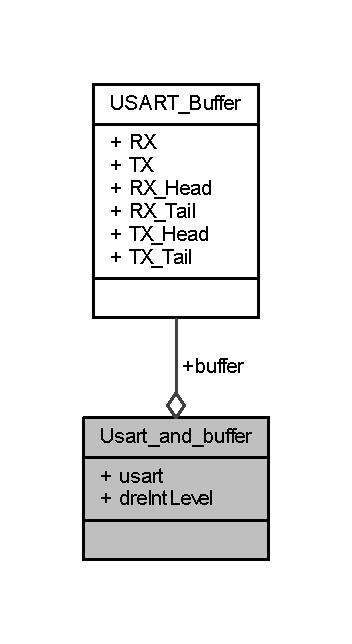
\includegraphics[width=169pt]{struct_usart__and__buffer__coll__graph}
\end{center}
\end{figure}
\subsection*{Data Fields}
\begin{DoxyCompactItemize}
\item 
U\+S\+A\+R\+T\+\_\+t $\ast$ \hyperlink{struct_usart__and__buffer_a5a819ee5e46999aaae5cb6813014ec08}{usart}
\item 
U\+S\+A\+R\+T\+\_\+\+D\+R\+E\+I\+N\+T\+L\+V\+L\+\_\+t \hyperlink{struct_usart__and__buffer_ad854f355ca0804e81a03cd57c659da59}{dre\+Int\+Level}
\item 
\hyperlink{usart__driver_8h_af27d135e807dcd1846b6f175997c5f45}{U\+S\+A\+R\+T\+\_\+\+Buffer\+\_\+t} \hyperlink{struct_usart__and__buffer_adb062fac585f93e6e48f3d5980e30f22}{buffer}
\end{DoxyCompactItemize}


\subsection{Detailed Description}
Struct used when interrupt driven driver is used. 

Struct containing pointer to a usart, a buffer and a location to store Data register interrupt level temporary. 

Definition at line 107 of file usart\+\_\+driver.\+h.



\subsection{Field Documentation}
\hypertarget{struct_usart__and__buffer_adb062fac585f93e6e48f3d5980e30f22}{}\label{struct_usart__and__buffer_adb062fac585f93e6e48f3d5980e30f22} 
\index{Usart\+\_\+and\+\_\+buffer@{Usart\+\_\+and\+\_\+buffer}!buffer@{buffer}}
\index{buffer@{buffer}!Usart\+\_\+and\+\_\+buffer@{Usart\+\_\+and\+\_\+buffer}}
\subsubsection{\texorpdfstring{buffer}{buffer}}
{\footnotesize\ttfamily \hyperlink{usart__driver_8h_af27d135e807dcd1846b6f175997c5f45}{U\+S\+A\+R\+T\+\_\+\+Buffer\+\_\+t} buffer}



Definition at line 114 of file usart\+\_\+driver.\+h.



Referenced by I\+S\+R(), U\+S\+A\+R\+T\+\_\+\+Data\+Reg\+Empty(), U\+S\+A\+R\+T\+\_\+\+Interrupt\+Driver\+\_\+\+Initialize(), U\+S\+A\+R\+T\+\_\+\+R\+X\+Buffer\+\_\+\+Get\+Byte(), U\+S\+A\+R\+T\+\_\+\+R\+X\+Buffer\+Data\+\_\+\+Available(), U\+S\+A\+R\+T\+\_\+\+R\+X\+Complete(), U\+S\+A\+R\+T\+\_\+test(), U\+S\+A\+R\+T\+\_\+\+T\+X\+Buffer\+\_\+\+Free\+Space(), and U\+S\+A\+R\+T\+\_\+\+T\+X\+Buffer\+\_\+\+Put\+Byte().

\hypertarget{struct_usart__and__buffer_ad854f355ca0804e81a03cd57c659da59}{}\label{struct_usart__and__buffer_ad854f355ca0804e81a03cd57c659da59} 
\index{Usart\+\_\+and\+\_\+buffer@{Usart\+\_\+and\+\_\+buffer}!dre\+Int\+Level@{dre\+Int\+Level}}
\index{dre\+Int\+Level@{dre\+Int\+Level}!Usart\+\_\+and\+\_\+buffer@{Usart\+\_\+and\+\_\+buffer}}
\subsubsection{\texorpdfstring{dre\+Int\+Level}{dreIntLevel}}
{\footnotesize\ttfamily U\+S\+A\+R\+T\+\_\+\+D\+R\+E\+I\+N\+T\+L\+V\+L\+\_\+t dre\+Int\+Level}



Definition at line 112 of file usart\+\_\+driver.\+h.



Referenced by U\+S\+A\+R\+T\+\_\+\+Interrupt\+Driver\+\_\+\+Dre\+Interrupt\+Level\+\_\+\+Set(), U\+S\+A\+R\+T\+\_\+\+Interrupt\+Driver\+\_\+\+Initialize(), and U\+S\+A\+R\+T\+\_\+\+T\+X\+Buffer\+\_\+\+Put\+Byte().

\hypertarget{struct_usart__and__buffer_a5a819ee5e46999aaae5cb6813014ec08}{}\label{struct_usart__and__buffer_a5a819ee5e46999aaae5cb6813014ec08} 
\index{Usart\+\_\+and\+\_\+buffer@{Usart\+\_\+and\+\_\+buffer}!usart@{usart}}
\index{usart@{usart}!Usart\+\_\+and\+\_\+buffer@{Usart\+\_\+and\+\_\+buffer}}
\subsubsection{\texorpdfstring{usart}{usart}}
{\footnotesize\ttfamily U\+S\+A\+R\+T\+\_\+t$\ast$ usart}



Definition at line 110 of file usart\+\_\+driver.\+h.



Referenced by U\+S\+A\+R\+T\+\_\+\+Data\+Reg\+Empty(), U\+S\+A\+R\+T\+\_\+\+Interrupt\+Driver\+\_\+\+Initialize(), U\+S\+A\+R\+T\+\_\+\+R\+X\+Complete(), and U\+S\+A\+R\+T\+\_\+\+T\+X\+Buffer\+\_\+\+Put\+Byte().



The documentation for this struct was generated from the following file\+:\begin{DoxyCompactItemize}
\item 
\hyperlink{usart__driver_8h}{usart\+\_\+driver.\+h}\end{DoxyCompactItemize}

\hypertarget{struct_u_s_a_r_t___buffer}{}\section{U\+S\+A\+R\+T\+\_\+\+Buffer Struct Reference}
\label{struct_u_s_a_r_t___buffer}\index{U\+S\+A\+R\+T\+\_\+\+Buffer@{U\+S\+A\+R\+T\+\_\+\+Buffer}}


{\ttfamily \#include \char`\"{}usart\+\_\+driver.\+h\char`\"{}}



Collaboration diagram for U\+S\+A\+R\+T\+\_\+\+Buffer\+:
% FIG 0
\subsection*{Data Fields}
\begin{DoxyCompactItemize}
\item 
volatile uint8\+\_\+t \hyperlink{struct_u_s_a_r_t___buffer_a3b83538f34138ed63ae42daeaa092639}{RX} \mbox{[}\hyperlink{usart__driver_8h_ac0999c0821d14cfab43e6f3c778c2b95}{U\+S\+A\+R\+T\+\_\+\+R\+X\+\_\+\+B\+U\+F\+F\+E\+R\+\_\+\+S\+I\+ZE}\mbox{]}
\item 
volatile uint8\+\_\+t \hyperlink{struct_u_s_a_r_t___buffer_a392312bfc5a33886fa4c6999cea21ecc}{TX} \mbox{[}\hyperlink{usart__driver_8h_a21d527450b438bba8dab02e03f021ee3}{U\+S\+A\+R\+T\+\_\+\+T\+X\+\_\+\+B\+U\+F\+F\+E\+R\+\_\+\+S\+I\+ZE}\mbox{]}
\item 
volatile uint8\+\_\+t \hyperlink{struct_u_s_a_r_t___buffer_aca7bb6ebcc2a3f266fac41649a250041}{R\+X\+\_\+\+Head}
\item 
volatile uint8\+\_\+t \hyperlink{struct_u_s_a_r_t___buffer_acbe55e05936cb836303c2fd41ec2d734}{R\+X\+\_\+\+Tail}
\item 
volatile uint8\+\_\+t \hyperlink{struct_u_s_a_r_t___buffer_ae18341a2700d746f90841b29ce8b05ca}{T\+X\+\_\+\+Head}
\item 
volatile uint8\+\_\+t \hyperlink{struct_u_s_a_r_t___buffer_ab4c125e286a5f36c1f44256fd35eb66d}{T\+X\+\_\+\+Tail}
\end{DoxyCompactItemize}


\subsection{Detailed Description}


Definition at line 85 of file usart\+\_\+driver.\+h.



\subsection{Field Documentation}
\hypertarget{struct_u_s_a_r_t___buffer_a3b83538f34138ed63ae42daeaa092639}{}\label{struct_u_s_a_r_t___buffer_a3b83538f34138ed63ae42daeaa092639} 
\index{U\+S\+A\+R\+T\+\_\+\+Buffer@{U\+S\+A\+R\+T\+\_\+\+Buffer}!RX@{RX}}
\index{RX@{RX}!U\+S\+A\+R\+T\+\_\+\+Buffer@{U\+S\+A\+R\+T\+\_\+\+Buffer}}
\subsubsection{\texorpdfstring{RX}{RX}}
{\footnotesize\ttfamily volatile uint8\+\_\+t RX\mbox{[}\hyperlink{usart__driver_8h_ac0999c0821d14cfab43e6f3c778c2b95}{U\+S\+A\+R\+T\+\_\+\+R\+X\+\_\+\+B\+U\+F\+F\+E\+R\+\_\+\+S\+I\+ZE}\mbox{]}}



Definition at line 88 of file usart\+\_\+driver.\+h.



Referenced by I\+S\+R(), U\+S\+A\+R\+T\+\_\+\+R\+X\+Buffer\+\_\+\+Get\+Byte(), U\+S\+A\+R\+T\+\_\+\+R\+X\+Complete(), and U\+S\+A\+R\+T\+\_\+test().

\hypertarget{struct_u_s_a_r_t___buffer_aca7bb6ebcc2a3f266fac41649a250041}{}\label{struct_u_s_a_r_t___buffer_aca7bb6ebcc2a3f266fac41649a250041} 
\index{U\+S\+A\+R\+T\+\_\+\+Buffer@{U\+S\+A\+R\+T\+\_\+\+Buffer}!R\+X\+\_\+\+Head@{R\+X\+\_\+\+Head}}
\index{R\+X\+\_\+\+Head@{R\+X\+\_\+\+Head}!U\+S\+A\+R\+T\+\_\+\+Buffer@{U\+S\+A\+R\+T\+\_\+\+Buffer}}
\subsubsection{\texorpdfstring{R\+X\+\_\+\+Head}{RX\_Head}}
{\footnotesize\ttfamily volatile uint8\+\_\+t R\+X\+\_\+\+Head}



Definition at line 92 of file usart\+\_\+driver.\+h.



Referenced by I\+S\+R(), U\+S\+A\+R\+T\+\_\+\+Interrupt\+Driver\+\_\+\+Initialize(), U\+S\+A\+R\+T\+\_\+\+R\+X\+Buffer\+Data\+\_\+\+Available(), and U\+S\+A\+R\+T\+\_\+\+R\+X\+Complete().

\hypertarget{struct_u_s_a_r_t___buffer_acbe55e05936cb836303c2fd41ec2d734}{}\label{struct_u_s_a_r_t___buffer_acbe55e05936cb836303c2fd41ec2d734} 
\index{U\+S\+A\+R\+T\+\_\+\+Buffer@{U\+S\+A\+R\+T\+\_\+\+Buffer}!R\+X\+\_\+\+Tail@{R\+X\+\_\+\+Tail}}
\index{R\+X\+\_\+\+Tail@{R\+X\+\_\+\+Tail}!U\+S\+A\+R\+T\+\_\+\+Buffer@{U\+S\+A\+R\+T\+\_\+\+Buffer}}
\subsubsection{\texorpdfstring{R\+X\+\_\+\+Tail}{RX\_Tail}}
{\footnotesize\ttfamily volatile uint8\+\_\+t R\+X\+\_\+\+Tail}



Definition at line 94 of file usart\+\_\+driver.\+h.



Referenced by U\+S\+A\+R\+T\+\_\+\+Interrupt\+Driver\+\_\+\+Initialize(), U\+S\+A\+R\+T\+\_\+\+R\+X\+Buffer\+\_\+\+Get\+Byte(), U\+S\+A\+R\+T\+\_\+\+R\+X\+Buffer\+Data\+\_\+\+Available(), U\+S\+A\+R\+T\+\_\+\+R\+X\+Complete(), and U\+S\+A\+R\+T\+\_\+test().

\hypertarget{struct_u_s_a_r_t___buffer_a392312bfc5a33886fa4c6999cea21ecc}{}\label{struct_u_s_a_r_t___buffer_a392312bfc5a33886fa4c6999cea21ecc} 
\index{U\+S\+A\+R\+T\+\_\+\+Buffer@{U\+S\+A\+R\+T\+\_\+\+Buffer}!TX@{TX}}
\index{TX@{TX}!U\+S\+A\+R\+T\+\_\+\+Buffer@{U\+S\+A\+R\+T\+\_\+\+Buffer}}
\subsubsection{\texorpdfstring{TX}{TX}}
{\footnotesize\ttfamily volatile uint8\+\_\+t TX\mbox{[}\hyperlink{usart__driver_8h_a21d527450b438bba8dab02e03f021ee3}{U\+S\+A\+R\+T\+\_\+\+T\+X\+\_\+\+B\+U\+F\+F\+E\+R\+\_\+\+S\+I\+ZE}\mbox{]}}



Definition at line 90 of file usart\+\_\+driver.\+h.



Referenced by U\+S\+A\+R\+T\+\_\+\+Data\+Reg\+Empty(), and U\+S\+A\+R\+T\+\_\+\+T\+X\+Buffer\+\_\+\+Put\+Byte().

\hypertarget{struct_u_s_a_r_t___buffer_ae18341a2700d746f90841b29ce8b05ca}{}\label{struct_u_s_a_r_t___buffer_ae18341a2700d746f90841b29ce8b05ca} 
\index{U\+S\+A\+R\+T\+\_\+\+Buffer@{U\+S\+A\+R\+T\+\_\+\+Buffer}!T\+X\+\_\+\+Head@{T\+X\+\_\+\+Head}}
\index{T\+X\+\_\+\+Head@{T\+X\+\_\+\+Head}!U\+S\+A\+R\+T\+\_\+\+Buffer@{U\+S\+A\+R\+T\+\_\+\+Buffer}}
\subsubsection{\texorpdfstring{T\+X\+\_\+\+Head}{TX\_Head}}
{\footnotesize\ttfamily volatile uint8\+\_\+t T\+X\+\_\+\+Head}



Definition at line 96 of file usart\+\_\+driver.\+h.



Referenced by U\+S\+A\+R\+T\+\_\+\+Data\+Reg\+Empty(), U\+S\+A\+R\+T\+\_\+\+Interrupt\+Driver\+\_\+\+Initialize(), U\+S\+A\+R\+T\+\_\+\+T\+X\+Buffer\+\_\+\+Free\+Space(), and U\+S\+A\+R\+T\+\_\+\+T\+X\+Buffer\+\_\+\+Put\+Byte().

\hypertarget{struct_u_s_a_r_t___buffer_ab4c125e286a5f36c1f44256fd35eb66d}{}\label{struct_u_s_a_r_t___buffer_ab4c125e286a5f36c1f44256fd35eb66d} 
\index{U\+S\+A\+R\+T\+\_\+\+Buffer@{U\+S\+A\+R\+T\+\_\+\+Buffer}!T\+X\+\_\+\+Tail@{T\+X\+\_\+\+Tail}}
\index{T\+X\+\_\+\+Tail@{T\+X\+\_\+\+Tail}!U\+S\+A\+R\+T\+\_\+\+Buffer@{U\+S\+A\+R\+T\+\_\+\+Buffer}}
\subsubsection{\texorpdfstring{T\+X\+\_\+\+Tail}{TX\_Tail}}
{\footnotesize\ttfamily volatile uint8\+\_\+t T\+X\+\_\+\+Tail}



Definition at line 98 of file usart\+\_\+driver.\+h.



Referenced by U\+S\+A\+R\+T\+\_\+\+Data\+Reg\+Empty(), U\+S\+A\+R\+T\+\_\+\+Interrupt\+Driver\+\_\+\+Initialize(), and U\+S\+A\+R\+T\+\_\+\+T\+X\+Buffer\+\_\+\+Free\+Space().



The documentation for this struct was generated from the following file\+:\begin{DoxyCompactItemize}
\item 
\hyperlink{usart__driver_8h}{usart\+\_\+driver.\+h}\end{DoxyCompactItemize}

\chapter{File Documentation}
\hypertarget{avr__compiler_8h}{}\section{avr\+\_\+compiler.\+h File Reference}
\label{avr__compiler_8h}\index{avr\+\_\+compiler.\+h@{avr\+\_\+compiler.\+h}}


This file implements some macros that makes the I\+AR C-\/compiler and avr-\/gcc work with the same code base for the A\+VR architecture.  


{\ttfamily \#include $<$stdint.\+h$>$}\newline
{\ttfamily \#include $<$stdbool.\+h$>$}\newline
{\ttfamily \#include $<$stdlib.\+h$>$}\newline
Include dependency graph for avr\+\_\+compiler.\+h\+:\nopagebreak
\begin{figure}[H]
\begin{center}
\leavevmode
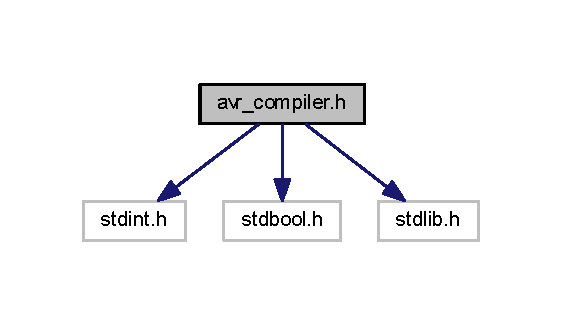
\includegraphics[width=270pt]{avr__compiler_8h__incl}
\end{center}
\end{figure}
This graph shows which files directly or indirectly include this file\+:\nopagebreak
\begin{figure}[H]
\begin{center}
\leavevmode
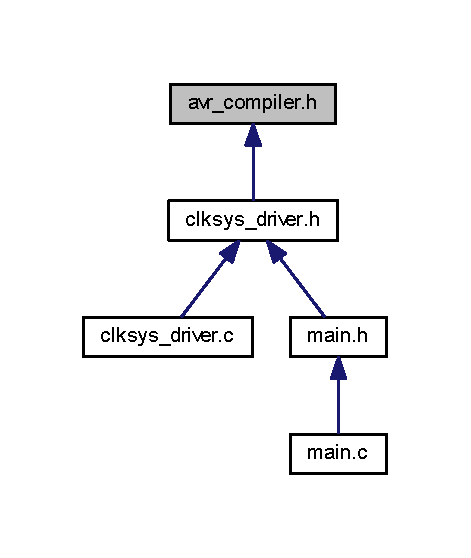
\includegraphics[width=226pt]{avr__compiler_8h__dep__incl}
\end{center}
\end{figure}
\subsection*{Macros}
\begin{DoxyCompactItemize}
\item 
\#define \hyperlink{avr__compiler_8h_a43bafb28b29491ec7f871319b5a3b2f8}{F\+\_\+\+C\+PU}~2000000\+UL
\begin{DoxyCompactList}\small\item\em Define default C\+PU frequency, if this is not already defined. \end{DoxyCompactList}\item 
\#define \hyperlink{avr__compiler_8h_a0a4fb62f9e69209c9c8c8e34ebb3df6f}{A\+V\+R\+\_\+\+E\+N\+T\+E\+R\+\_\+\+C\+R\+I\+T\+I\+C\+A\+L\+\_\+\+R\+E\+G\+I\+ON}()
\begin{DoxyCompactList}\small\item\em This macro will protect the following code from interrupts. \end{DoxyCompactList}\item 
\#define \hyperlink{avr__compiler_8h_a770b47b04eec57748be0826a3d23503b}{A\+V\+R\+\_\+\+L\+E\+A\+V\+E\+\_\+\+C\+R\+I\+T\+I\+C\+A\+L\+\_\+\+R\+E\+G\+I\+ON}()~S\+R\+EG = saved\+\_\+sreg;
\begin{DoxyCompactList}\small\item\em This macro must always be used in conjunction with A\+V\+R\+\_\+\+E\+N\+T\+E\+R\+\_\+\+C\+R\+I\+T\+I\+C\+A\+L\+\_\+\+R\+E\+G\+I\+ON so the interrupts are enabled again. \end{DoxyCompactList}\end{DoxyCompactItemize}


\subsection{Detailed Description}
This file implements some macros that makes the I\+AR C-\/compiler and avr-\/gcc work with the same code base for the A\+VR architecture. 

\begin{DoxyParagraph}{Documentation}
For comprehensive code documentation, supported compilers, compiler settings and supported devices see readme.\+html
\end{DoxyParagraph}
\begin{DoxyAuthor}{Author}
Atmel Corporation\+: \href{http://www.atmel.com}{\tt http\+://www.\+atmel.\+com} ~\newline
 Support email\+: \href{mailto:avr@atmel.com}{\tt avr@atmel.\+com}
\end{DoxyAuthor}
\begin{DoxyParagraph}{Revision}
2772 
\end{DoxyParagraph}
\begin{DoxyParagraph}{Date}
2009-\/09-\/11 12\+:40\+:26 +0200 (fr, 11 sep 2009) 
\end{DoxyParagraph}
~\newline
 Copyright (c) 2008, Atmel Corporation All rights reserved.

Redistribution and use in source and binary forms, with or without modification, are permitted provided that the following conditions are met\+:


\begin{DoxyEnumerate}
\item Redistributions of source code must retain the above copyright notice, this list of conditions and the following disclaimer.
\item Redistributions in binary form must reproduce the above copyright notice, this list of conditions and the following disclaimer in the documentation and/or other materials provided with the distribution.
\item The name of A\+T\+M\+EL may not be used to endorse or promote products derived from this software without specific prior written permission.
\end{DoxyEnumerate}

T\+H\+IS S\+O\+F\+T\+W\+A\+RE IS P\+R\+O\+V\+I\+D\+ED BY A\+T\+M\+EL \char`\"{}\+A\+S I\+S\char`\"{} A\+ND A\+NY E\+X\+P\+R\+E\+SS OR I\+M\+P\+L\+I\+ED W\+A\+R\+R\+A\+N\+T\+I\+ES, I\+N\+C\+L\+U\+D\+I\+NG, B\+UT N\+OT L\+I\+M\+I\+T\+ED TO, T\+HE I\+M\+P\+L\+I\+ED W\+A\+R\+R\+A\+N\+T\+I\+ES OF M\+E\+R\+C\+H\+A\+N\+T\+A\+B\+I\+L\+I\+TY A\+ND F\+I\+T\+N\+E\+SS F\+OR A P\+A\+R\+T\+I\+C\+U\+L\+AR P\+U\+R\+P\+O\+SE A\+RE E\+X\+P\+R\+E\+S\+S\+LY A\+ND S\+P\+E\+C\+I\+F\+I\+C\+A\+L\+LY D\+I\+S\+C\+L\+A\+I\+M\+ED. IN NO E\+V\+E\+NT S\+H\+A\+LL A\+T\+M\+EL BE L\+I\+A\+B\+LE F\+OR A\+NY D\+I\+R\+E\+CT, I\+N\+D\+I\+R\+E\+CT, I\+N\+C\+I\+D\+E\+N\+T\+AL, S\+P\+E\+C\+I\+AL, E\+X\+E\+M\+P\+L\+A\+RY, OR C\+O\+N\+S\+E\+Q\+U\+E\+N\+T\+I\+AL D\+A\+M\+A\+G\+ES (I\+N\+C\+L\+U\+D\+I\+NG, B\+UT N\+OT L\+I\+M\+I\+T\+ED TO, P\+R\+O\+C\+U\+R\+E\+M\+E\+NT OF S\+U\+B\+S\+T\+I\+T\+U\+TE G\+O\+O\+DS OR S\+E\+R\+V\+I\+C\+ES; L\+O\+SS OF U\+SE, D\+A\+TA, OR P\+R\+O\+F\+I\+TS; OR B\+U\+S\+I\+N\+E\+SS I\+N\+T\+E\+R\+R\+U\+P\+T\+I\+ON) H\+O\+W\+E\+V\+ER C\+A\+U\+S\+ED A\+ND ON A\+NY T\+H\+E\+O\+RY OF L\+I\+A\+B\+I\+L\+I\+TY, W\+H\+E\+T\+H\+ER IN C\+O\+N\+T\+R\+A\+CT, S\+T\+R\+I\+CT L\+I\+A\+B\+I\+L\+I\+TY, OR T\+O\+RT (I\+N\+C\+L\+U\+D\+I\+NG N\+E\+G\+L\+I\+G\+E\+N\+CE OR O\+T\+H\+E\+R\+W\+I\+SE) A\+R\+I\+S\+I\+NG IN A\+NY W\+AY O\+UT OF T\+HE U\+SE OF T\+H\+IS S\+O\+F\+T\+W\+A\+RE, E\+V\+EN IF A\+D\+V\+I\+S\+ED OF T\+HE P\+O\+S\+S\+I\+B\+I\+L\+I\+TY OF S\+U\+CH D\+A\+M\+A\+GE. 

\subsection{Macro Definition Documentation}
\hypertarget{avr__compiler_8h_a0a4fb62f9e69209c9c8c8e34ebb3df6f}{}\label{avr__compiler_8h_a0a4fb62f9e69209c9c8c8e34ebb3df6f} 
\index{avr\+\_\+compiler.\+h@{avr\+\_\+compiler.\+h}!A\+V\+R\+\_\+\+E\+N\+T\+E\+R\+\_\+\+C\+R\+I\+T\+I\+C\+A\+L\+\_\+\+R\+E\+G\+I\+ON@{A\+V\+R\+\_\+\+E\+N\+T\+E\+R\+\_\+\+C\+R\+I\+T\+I\+C\+A\+L\+\_\+\+R\+E\+G\+I\+ON}}
\index{A\+V\+R\+\_\+\+E\+N\+T\+E\+R\+\_\+\+C\+R\+I\+T\+I\+C\+A\+L\+\_\+\+R\+E\+G\+I\+ON@{A\+V\+R\+\_\+\+E\+N\+T\+E\+R\+\_\+\+C\+R\+I\+T\+I\+C\+A\+L\+\_\+\+R\+E\+G\+I\+ON}!avr\+\_\+compiler.\+h@{avr\+\_\+compiler.\+h}}
\subsubsection{\texorpdfstring{A\+V\+R\+\_\+\+E\+N\+T\+E\+R\+\_\+\+C\+R\+I\+T\+I\+C\+A\+L\+\_\+\+R\+E\+G\+I\+ON}{AVR\_ENTER\_CRITICAL\_REGION}}
{\footnotesize\ttfamily \#define A\+V\+R\+\_\+\+E\+N\+T\+E\+R\+\_\+\+C\+R\+I\+T\+I\+C\+A\+L\+\_\+\+R\+E\+G\+I\+ON(\begin{DoxyParamCaption}{ }\end{DoxyParamCaption})}

{\bfseries Value\+:}
\begin{DoxyCode}
uint8\_t \textcolor{keyword}{volatile} saved\_sreg = SREG; \(\backslash\)
                                     cli();
\end{DoxyCode}


This macro will protect the following code from interrupts. 



Definition at line 58 of file avr\+\_\+compiler.\+h.



Referenced by C\+C\+P\+Write().

\hypertarget{avr__compiler_8h_a770b47b04eec57748be0826a3d23503b}{}\label{avr__compiler_8h_a770b47b04eec57748be0826a3d23503b} 
\index{avr\+\_\+compiler.\+h@{avr\+\_\+compiler.\+h}!A\+V\+R\+\_\+\+L\+E\+A\+V\+E\+\_\+\+C\+R\+I\+T\+I\+C\+A\+L\+\_\+\+R\+E\+G\+I\+ON@{A\+V\+R\+\_\+\+L\+E\+A\+V\+E\+\_\+\+C\+R\+I\+T\+I\+C\+A\+L\+\_\+\+R\+E\+G\+I\+ON}}
\index{A\+V\+R\+\_\+\+L\+E\+A\+V\+E\+\_\+\+C\+R\+I\+T\+I\+C\+A\+L\+\_\+\+R\+E\+G\+I\+ON@{A\+V\+R\+\_\+\+L\+E\+A\+V\+E\+\_\+\+C\+R\+I\+T\+I\+C\+A\+L\+\_\+\+R\+E\+G\+I\+ON}!avr\+\_\+compiler.\+h@{avr\+\_\+compiler.\+h}}
\subsubsection{\texorpdfstring{A\+V\+R\+\_\+\+L\+E\+A\+V\+E\+\_\+\+C\+R\+I\+T\+I\+C\+A\+L\+\_\+\+R\+E\+G\+I\+ON}{AVR\_LEAVE\_CRITICAL\_REGION}}
{\footnotesize\ttfamily \#define A\+V\+R\+\_\+\+L\+E\+A\+V\+E\+\_\+\+C\+R\+I\+T\+I\+C\+A\+L\+\_\+\+R\+E\+G\+I\+ON(\begin{DoxyParamCaption}{ }\end{DoxyParamCaption})~S\+R\+EG = saved\+\_\+sreg;}



This macro must always be used in conjunction with A\+V\+R\+\_\+\+E\+N\+T\+E\+R\+\_\+\+C\+R\+I\+T\+I\+C\+A\+L\+\_\+\+R\+E\+G\+I\+ON so the interrupts are enabled again. 



Definition at line 64 of file avr\+\_\+compiler.\+h.



Referenced by C\+C\+P\+Write().

\hypertarget{avr__compiler_8h_a43bafb28b29491ec7f871319b5a3b2f8}{}\label{avr__compiler_8h_a43bafb28b29491ec7f871319b5a3b2f8} 
\index{avr\+\_\+compiler.\+h@{avr\+\_\+compiler.\+h}!F\+\_\+\+C\+PU@{F\+\_\+\+C\+PU}}
\index{F\+\_\+\+C\+PU@{F\+\_\+\+C\+PU}!avr\+\_\+compiler.\+h@{avr\+\_\+compiler.\+h}}
\subsubsection{\texorpdfstring{F\+\_\+\+C\+PU}{F\_CPU}}
{\footnotesize\ttfamily \#define F\+\_\+\+C\+PU~2000000\+UL}



Define default C\+PU frequency, if this is not already defined. 



Definition at line 50 of file avr\+\_\+compiler.\+h.


\hypertarget{clksys__driver_8c}{}\section{clksys\+\_\+driver.\+c File Reference}
\label{clksys__driver_8c}\index{clksys\+\_\+driver.\+c@{clksys\+\_\+driver.\+c}}


X\+M\+E\+GA Clock System driver source file.  


{\ttfamily \#include \char`\"{}clksys\+\_\+driver.\+h\char`\"{}}\newline
Include dependency graph for clksys\+\_\+driver.\+c\+:\nopagebreak
\begin{figure}[H]
\begin{center}
\leavevmode
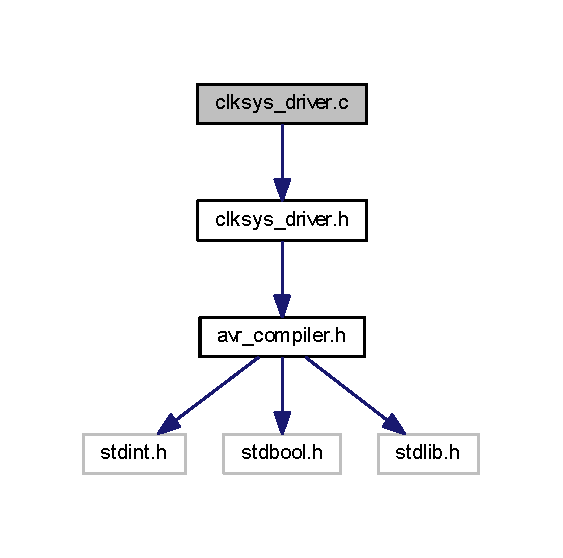
\includegraphics[width=270pt]{clksys__driver_8c__incl}
\end{center}
\end{figure}
\subsection*{Functions}
\begin{DoxyCompactItemize}
\item 
void \hyperlink{clksys__driver_8c_aad4e162434c2cc7e0087bbc0ddfe266c}{C\+C\+P\+Write} (volatile uint8\+\_\+t $\ast$address, uint8\+\_\+t value)
\begin{DoxyCompactList}\small\item\em C\+CP write helper function written in assembly. \end{DoxyCompactList}\item 
void \hyperlink{clksys__driver_8c_ace371b352e90117520436eb125aeeec0}{C\+L\+K\+S\+Y\+S\+\_\+\+X\+O\+S\+C\+\_\+\+Config} (O\+S\+C\+\_\+\+F\+R\+Q\+R\+A\+N\+G\+E\+\_\+t freq\+Range, bool low\+Power32k\+Hz, O\+S\+C\+\_\+\+X\+O\+S\+C\+S\+E\+L\+\_\+t xosc\+Mode\+Selection)
\begin{DoxyCompactList}\small\item\em This function configures the external oscillator. \end{DoxyCompactList}\item 
void \hyperlink{clksys__driver_8c_acb82744003806825da7fb6a7bb973941}{C\+L\+K\+S\+Y\+S\+\_\+\+P\+L\+L\+\_\+\+Config} (O\+S\+C\+\_\+\+P\+L\+L\+S\+R\+C\+\_\+t clock\+Source, uint8\+\_\+t factor)
\begin{DoxyCompactList}\small\item\em This function configures the internal high-\/frequency P\+LL. \end{DoxyCompactList}\item 
uint8\+\_\+t \hyperlink{clksys__driver_8c_a31b1ca1994b6a687974a119d1ad8008c}{C\+L\+K\+S\+Y\+S\+\_\+\+Disable} (uint8\+\_\+t osc\+Sel)
\begin{DoxyCompactList}\small\item\em This function disables the selected oscillator. \end{DoxyCompactList}\item 
void \hyperlink{clksys__driver_8c_a8e350b689dc409a4c9b902a192d1e8a3}{C\+L\+K\+S\+Y\+S\+\_\+\+Prescalers\+\_\+\+Config} (C\+L\+K\+\_\+\+P\+S\+A\+D\+I\+V\+\_\+t P\+S\+Afactor, C\+L\+K\+\_\+\+P\+S\+B\+C\+D\+I\+V\+\_\+t P\+S\+B\+Cfactor)
\begin{DoxyCompactList}\small\item\em This function changes the prescaler configuration. \end{DoxyCompactList}\item 
uint8\+\_\+t \hyperlink{clksys__driver_8c_a1e46c4a8f01a83d4e4747d32d113e7e2}{C\+L\+K\+S\+Y\+S\+\_\+\+Main\+\_\+\+Clock\+Source\+\_\+\+Select} (C\+L\+K\+\_\+\+S\+C\+L\+K\+S\+E\+L\+\_\+t clock\+Source)
\begin{DoxyCompactList}\small\item\em This function selects the main system clock source. \end{DoxyCompactList}\item 
void \hyperlink{clksys__driver_8c_ae622e3056cd713fdca464b9fd6e5a7ab}{C\+L\+K\+S\+Y\+S\+\_\+\+R\+T\+C\+\_\+\+Clock\+Source\+\_\+\+Enable} (C\+L\+K\+\_\+\+R\+T\+C\+S\+R\+C\+\_\+t clock\+Source)
\begin{DoxyCompactList}\small\item\em This function selects a Real-\/\+Time Counter clock source. \end{DoxyCompactList}\item 
void \hyperlink{clksys__driver_8c_a581c15c6c0b2eaa0c81f0b5cafc3b82d}{C\+L\+K\+S\+Y\+S\+\_\+\+Auto\+Calibration\+\_\+\+Enable} (uint8\+\_\+t clk\+Source, bool ext\+Reference)
\begin{DoxyCompactList}\small\item\em This function enables automatic calibration of the selected internal oscillator. \end{DoxyCompactList}\item 
void \hyperlink{clksys__driver_8c_abfb0da2d81736412af825d46e7e0cedb}{C\+L\+K\+S\+Y\+S\+\_\+\+X\+O\+S\+C\+\_\+\+Failure\+Detection\+\_\+\+Enable} (void)
\begin{DoxyCompactList}\small\item\em This function enables the External Oscillator Failure Detection (X\+O\+S\+C\+FD) feature. \end{DoxyCompactList}\item 
void \hyperlink{clksys__driver_8c_a6225fea8fc405c6d1dab88d0ad537173}{C\+L\+K\+S\+Y\+S\+\_\+\+Configuration\+\_\+\+Lock} (void)
\begin{DoxyCompactList}\small\item\em This function lock the entire clock system configuration. \end{DoxyCompactList}\end{DoxyCompactItemize}


\subsection{Detailed Description}
X\+M\+E\+GA Clock System driver source file. 

This file contains the function implementations for the X\+M\+E\+GA Clock System driver.

The driver is not intended for size and/or speed critical code, since most functions are just a few lines of code, and the function call overhead would decrease code performance. The driver is intended for rapid prototyping and documentation purposes for getting started with the X\+M\+E\+GA Clock System.

For size and/or speed critical code, it is recommended to copy the function contents directly into your application instead of making a function call.

Several functions use the following construct\+: \char`\"{}some\+\_\+register = ... $\vert$ (some\+\_\+parameter ? S\+O\+M\+E\+\_\+\+B\+I\+T\+\_\+bm \+: 0) $\vert$ ...\char`\"{} Although the use of the ternary operator ( if ? then \+: else ) is discouraged, in some occasions the operator makes it possible to write pretty clean and neat code. In this driver, the construct is used to set or not set a configuration bit based on a boolean input parameter, such as the \char`\"{}some\+\_\+parameter\char`\"{} in the example above.

\begin{DoxyParagraph}{Application note\+:}
A\+V\+R1003\+: Using the X\+M\+E\+GA Clock System
\end{DoxyParagraph}
\begin{DoxyParagraph}{Documentation}
For comprehensive code documentation, supported compilers, compiler settings and supported devices see readme.\+html
\end{DoxyParagraph}
\begin{DoxyAuthor}{Author}
Atmel Corporation\+: \href{http://www.atmel.com}{\tt http\+://www.\+atmel.\+com} ~\newline
 Support email\+: \href{mailto:avr@atmel.com}{\tt avr@atmel.\+com}
\end{DoxyAuthor}
\begin{DoxyParagraph}{Revision}
2771 
\end{DoxyParagraph}
\begin{DoxyParagraph}{Date}
2009-\/09-\/11 11\+:54\+:26 +0200 (fr, 11 sep 2009) 
\end{DoxyParagraph}
~\newline
 Copyright (c) 2008, Atmel Corporation All rights reserved.

Redistribution and use in source and binary forms, with or without modification, are permitted provided that the following conditions are met\+:


\begin{DoxyEnumerate}
\item Redistributions of source code must retain the above copyright notice, this list of conditions and the following disclaimer.
\item Redistributions in binary form must reproduce the above copyright notice, this list of conditions and the following disclaimer in the documentation and/or other materials provided with the distribution.
\item The name of A\+T\+M\+EL may not be used to endorse or promote products derived from this software without specific prior written permission.
\end{DoxyEnumerate}

T\+H\+IS S\+O\+F\+T\+W\+A\+RE IS P\+R\+O\+V\+I\+D\+ED BY A\+T\+M\+EL \char`\"{}\+A\+S I\+S\char`\"{} A\+ND A\+NY E\+X\+P\+R\+E\+SS OR I\+M\+P\+L\+I\+ED W\+A\+R\+R\+A\+N\+T\+I\+ES, I\+N\+C\+L\+U\+D\+I\+NG, B\+UT N\+OT L\+I\+M\+I\+T\+ED TO, T\+HE I\+M\+P\+L\+I\+ED W\+A\+R\+R\+A\+N\+T\+I\+ES OF M\+E\+R\+C\+H\+A\+N\+T\+A\+B\+I\+L\+I\+TY A\+ND F\+I\+T\+N\+E\+SS F\+OR A P\+A\+R\+T\+I\+C\+U\+L\+AR P\+U\+R\+P\+O\+SE A\+RE E\+X\+P\+R\+E\+S\+S\+LY A\+ND S\+P\+E\+C\+I\+F\+I\+C\+A\+L\+LY D\+I\+S\+C\+L\+A\+I\+M\+ED. IN NO E\+V\+E\+NT S\+H\+A\+LL A\+T\+M\+EL BE L\+I\+A\+B\+LE F\+OR A\+NY D\+I\+R\+E\+CT, I\+N\+D\+I\+R\+E\+CT, I\+N\+C\+I\+D\+E\+N\+T\+AL, S\+P\+E\+C\+I\+AL, E\+X\+E\+M\+P\+L\+A\+RY, OR C\+O\+N\+S\+E\+Q\+U\+E\+N\+T\+I\+AL D\+A\+M\+A\+G\+ES (I\+N\+C\+L\+U\+D\+I\+NG, B\+UT N\+OT L\+I\+M\+I\+T\+ED TO, P\+R\+O\+C\+U\+R\+E\+M\+E\+NT OF S\+U\+B\+S\+T\+I\+T\+U\+TE G\+O\+O\+DS OR S\+E\+R\+V\+I\+C\+ES; L\+O\+SS OF U\+SE, D\+A\+TA, OR P\+R\+O\+F\+I\+TS; OR B\+U\+S\+I\+N\+E\+SS I\+N\+T\+E\+R\+R\+U\+P\+T\+I\+ON) H\+O\+W\+E\+V\+ER C\+A\+U\+S\+ED A\+ND ON A\+NY T\+H\+E\+O\+RY OF L\+I\+A\+B\+I\+L\+I\+TY, W\+H\+E\+T\+H\+ER IN C\+O\+N\+T\+R\+A\+CT, S\+T\+R\+I\+CT L\+I\+A\+B\+I\+L\+I\+TY, OR T\+O\+RT (I\+N\+C\+L\+U\+D\+I\+NG N\+E\+G\+L\+I\+G\+E\+N\+CE OR O\+T\+H\+E\+R\+W\+I\+SE) A\+R\+I\+S\+I\+NG IN A\+NY W\+AY O\+UT OF T\+HE U\+SE OF T\+H\+IS S\+O\+F\+T\+W\+A\+RE, E\+V\+EN IF A\+D\+V\+I\+S\+ED OF T\+HE P\+O\+S\+S\+I\+B\+I\+L\+I\+TY OF S\+U\+CH D\+A\+M\+A\+GE. 

\subsection{Function Documentation}
\hypertarget{clksys__driver_8c_aad4e162434c2cc7e0087bbc0ddfe266c}{}\label{clksys__driver_8c_aad4e162434c2cc7e0087bbc0ddfe266c} 
\index{clksys\+\_\+driver.\+c@{clksys\+\_\+driver.\+c}!C\+C\+P\+Write@{C\+C\+P\+Write}}
\index{C\+C\+P\+Write@{C\+C\+P\+Write}!clksys\+\_\+driver.\+c@{clksys\+\_\+driver.\+c}}
\subsubsection{\texorpdfstring{C\+C\+P\+Write()}{CCPWrite()}}
{\footnotesize\ttfamily void C\+C\+P\+Write (\begin{DoxyParamCaption}\item[{volatile uint8\+\_\+t $\ast$}]{address,  }\item[{uint8\+\_\+t}]{value }\end{DoxyParamCaption})}



C\+CP write helper function written in assembly. 

This function is written in assembly because of the timecritial operation of writing to the registers.


\begin{DoxyParams}{Parameters}
{\em address} & A pointer to the address to write to. \\
\hline
{\em value} & The value to put in to the register. \\
\hline
\end{DoxyParams}


Definition at line 77 of file clksys\+\_\+driver.\+c.



References A\+V\+R\+\_\+\+E\+N\+T\+E\+R\+\_\+\+C\+R\+I\+T\+I\+C\+A\+L\+\_\+\+R\+E\+G\+I\+ON, and A\+V\+R\+\_\+\+L\+E\+A\+V\+E\+\_\+\+C\+R\+I\+T\+I\+C\+A\+L\+\_\+\+R\+E\+G\+I\+ON.



Referenced by C\+L\+K\+S\+Y\+S\+\_\+\+Configuration\+\_\+\+Lock(), C\+L\+K\+S\+Y\+S\+\_\+\+Main\+\_\+\+Clock\+Source\+\_\+\+Select(), C\+L\+K\+S\+Y\+S\+\_\+\+Prescalers\+\_\+\+Config(), and C\+L\+K\+S\+Y\+S\+\_\+\+X\+O\+S\+C\+\_\+\+Failure\+Detection\+\_\+\+Enable().

Here is the caller graph for this function\+:\nopagebreak
\begin{figure}[H]
\begin{center}
\leavevmode
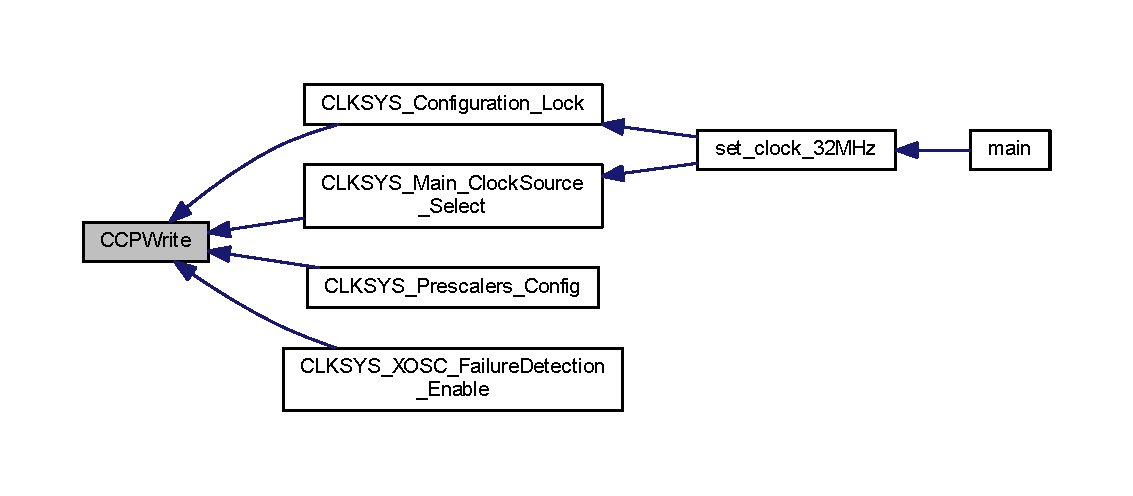
\includegraphics[width=350pt]{clksys__driver_8c_aad4e162434c2cc7e0087bbc0ddfe266c_icgraph}
\end{center}
\end{figure}
\hypertarget{clksys__driver_8c_a581c15c6c0b2eaa0c81f0b5cafc3b82d}{}\label{clksys__driver_8c_a581c15c6c0b2eaa0c81f0b5cafc3b82d} 
\index{clksys\+\_\+driver.\+c@{clksys\+\_\+driver.\+c}!C\+L\+K\+S\+Y\+S\+\_\+\+Auto\+Calibration\+\_\+\+Enable@{C\+L\+K\+S\+Y\+S\+\_\+\+Auto\+Calibration\+\_\+\+Enable}}
\index{C\+L\+K\+S\+Y\+S\+\_\+\+Auto\+Calibration\+\_\+\+Enable@{C\+L\+K\+S\+Y\+S\+\_\+\+Auto\+Calibration\+\_\+\+Enable}!clksys\+\_\+driver.\+c@{clksys\+\_\+driver.\+c}}
\subsubsection{\texorpdfstring{C\+L\+K\+S\+Y\+S\+\_\+\+Auto\+Calibration\+\_\+\+Enable()}{CLKSYS\_AutoCalibration\_Enable()}}
{\footnotesize\ttfamily void C\+L\+K\+S\+Y\+S\+\_\+\+Auto\+Calibration\+\_\+\+Enable (\begin{DoxyParamCaption}\item[{uint8\+\_\+t}]{clk\+Source,  }\item[{bool}]{ext\+Reference }\end{DoxyParamCaption})}



This function enables automatic calibration of the selected internal oscillator. 

Either the internal 32k\+Hz RC oscillator or an external 32k\+Hz crystal can be used as a calibration reference. The user must make sure that the selected reference is ready and running.


\begin{DoxyParams}{Parameters}
{\em clk\+Source} & Clock source to calibrate, either O\+S\+C\+\_\+\+R\+C2\+M\+C\+R\+E\+F\+\_\+bm or O\+S\+C\+\_\+\+R\+C32\+M\+C\+R\+E\+F\+\_\+gm -\/ patched to group mask(jb). \\
\hline
{\em ext\+Reference} & True if external crystal should be used as reference. \\
\hline
\end{DoxyParams}


Definition at line 260 of file clksys\+\_\+driver.\+c.



Referenced by set\+\_\+clock\+\_\+32\+M\+Hz().

Here is the caller graph for this function\+:\nopagebreak
\begin{figure}[H]
\begin{center}
\leavevmode
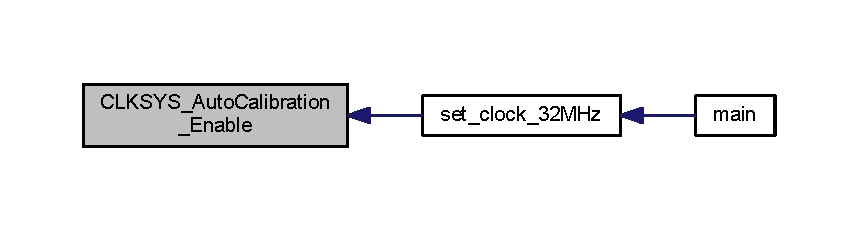
\includegraphics[width=350pt]{clksys__driver_8c_a581c15c6c0b2eaa0c81f0b5cafc3b82d_icgraph}
\end{center}
\end{figure}
\hypertarget{clksys__driver_8c_a6225fea8fc405c6d1dab88d0ad537173}{}\label{clksys__driver_8c_a6225fea8fc405c6d1dab88d0ad537173} 
\index{clksys\+\_\+driver.\+c@{clksys\+\_\+driver.\+c}!C\+L\+K\+S\+Y\+S\+\_\+\+Configuration\+\_\+\+Lock@{C\+L\+K\+S\+Y\+S\+\_\+\+Configuration\+\_\+\+Lock}}
\index{C\+L\+K\+S\+Y\+S\+\_\+\+Configuration\+\_\+\+Lock@{C\+L\+K\+S\+Y\+S\+\_\+\+Configuration\+\_\+\+Lock}!clksys\+\_\+driver.\+c@{clksys\+\_\+driver.\+c}}
\subsubsection{\texorpdfstring{C\+L\+K\+S\+Y\+S\+\_\+\+Configuration\+\_\+\+Lock()}{CLKSYS\_Configuration\_Lock()}}
{\footnotesize\ttfamily void C\+L\+K\+S\+Y\+S\+\_\+\+Configuration\+\_\+\+Lock (\begin{DoxyParamCaption}\item[{void}]{ }\end{DoxyParamCaption})}



This function lock the entire clock system configuration. 

This will lock the configuration until the next reset, or until the External Oscillator Failure Detections (X\+O\+S\+C\+FD) feature detects a failure and switches to internal 2\+M\+Hz RC oscillator. 

Definition at line 292 of file clksys\+\_\+driver.\+c.



References C\+C\+P\+Write().



Referenced by set\+\_\+clock\+\_\+32\+M\+Hz().

Here is the call graph for this function\+:\nopagebreak
\begin{figure}[H]
\begin{center}
\leavevmode
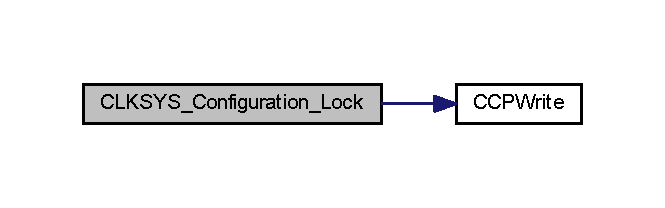
\includegraphics[width=319pt]{clksys__driver_8c_a6225fea8fc405c6d1dab88d0ad537173_cgraph}
\end{center}
\end{figure}
Here is the caller graph for this function\+:\nopagebreak
\begin{figure}[H]
\begin{center}
\leavevmode
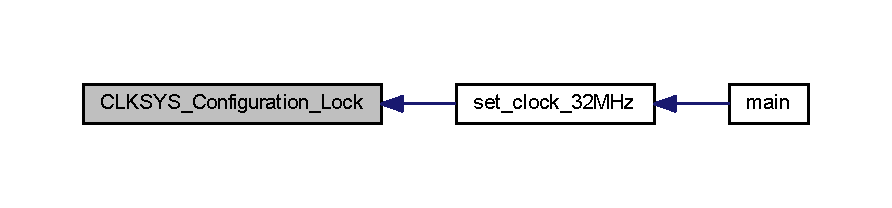
\includegraphics[width=350pt]{clksys__driver_8c_a6225fea8fc405c6d1dab88d0ad537173_icgraph}
\end{center}
\end{figure}
\hypertarget{clksys__driver_8c_a31b1ca1994b6a687974a119d1ad8008c}{}\label{clksys__driver_8c_a31b1ca1994b6a687974a119d1ad8008c} 
\index{clksys\+\_\+driver.\+c@{clksys\+\_\+driver.\+c}!C\+L\+K\+S\+Y\+S\+\_\+\+Disable@{C\+L\+K\+S\+Y\+S\+\_\+\+Disable}}
\index{C\+L\+K\+S\+Y\+S\+\_\+\+Disable@{C\+L\+K\+S\+Y\+S\+\_\+\+Disable}!clksys\+\_\+driver.\+c@{clksys\+\_\+driver.\+c}}
\subsubsection{\texorpdfstring{C\+L\+K\+S\+Y\+S\+\_\+\+Disable()}{CLKSYS\_Disable()}}
{\footnotesize\ttfamily uint8\+\_\+t C\+L\+K\+S\+Y\+S\+\_\+\+Disable (\begin{DoxyParamCaption}\item[{uint8\+\_\+t}]{osc\+Sel }\end{DoxyParamCaption})}



This function disables the selected oscillator. 

This function will disable the selected oscillator if possible. If it is currently used as a main system clock source, hardware will disregard the disable attempt, and this function will return zero. If it fails, change to another main system clock source and try again.


\begin{DoxyParams}{Parameters}
{\em osc\+Sel} & Bitmask of selected clock. Can be one of the following O\+S\+C\+\_\+\+R\+C2\+M\+E\+N\+\_\+bm, O\+S\+C\+\_\+\+R\+C32\+M\+E\+N\+\_\+bm, O\+S\+C\+\_\+\+R\+C32\+K\+E\+N\+\_\+bm, O\+S\+C\+\_\+\+X\+O\+S\+C\+E\+N\+\_\+bm, O\+S\+C\+\_\+\+P\+L\+L\+E\+N\+\_\+bm.\\
\hline
\end{DoxyParams}
\begin{DoxyReturn}{Returns}
Non-\/zero if oscillator was disabled successfully. 
\end{DoxyReturn}


Definition at line 187 of file clksys\+\_\+driver.\+c.



Referenced by set\+\_\+clock\+\_\+32\+M\+Hz().

Here is the caller graph for this function\+:\nopagebreak
\begin{figure}[H]
\begin{center}
\leavevmode
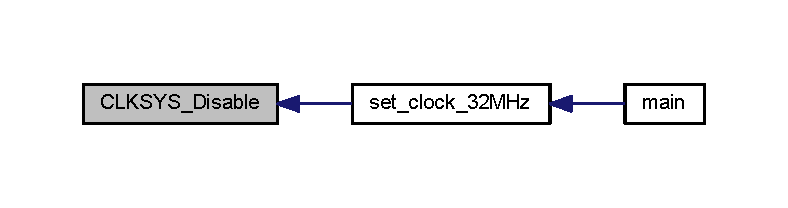
\includegraphics[width=350pt]{clksys__driver_8c_a31b1ca1994b6a687974a119d1ad8008c_icgraph}
\end{center}
\end{figure}
\hypertarget{clksys__driver_8c_a1e46c4a8f01a83d4e4747d32d113e7e2}{}\label{clksys__driver_8c_a1e46c4a8f01a83d4e4747d32d113e7e2} 
\index{clksys\+\_\+driver.\+c@{clksys\+\_\+driver.\+c}!C\+L\+K\+S\+Y\+S\+\_\+\+Main\+\_\+\+Clock\+Source\+\_\+\+Select@{C\+L\+K\+S\+Y\+S\+\_\+\+Main\+\_\+\+Clock\+Source\+\_\+\+Select}}
\index{C\+L\+K\+S\+Y\+S\+\_\+\+Main\+\_\+\+Clock\+Source\+\_\+\+Select@{C\+L\+K\+S\+Y\+S\+\_\+\+Main\+\_\+\+Clock\+Source\+\_\+\+Select}!clksys\+\_\+driver.\+c@{clksys\+\_\+driver.\+c}}
\subsubsection{\texorpdfstring{C\+L\+K\+S\+Y\+S\+\_\+\+Main\+\_\+\+Clock\+Source\+\_\+\+Select()}{CLKSYS\_Main\_ClockSource\_Select()}}
{\footnotesize\ttfamily uint8\+\_\+t C\+L\+K\+S\+Y\+S\+\_\+\+Main\+\_\+\+Clock\+Source\+\_\+\+Select (\begin{DoxyParamCaption}\item[{C\+L\+K\+\_\+\+S\+C\+L\+K\+S\+E\+L\+\_\+t}]{clock\+Source }\end{DoxyParamCaption})}



This function selects the main system clock source. 

Hardware will disregard any attempts to select a clock source that is not enabled or not stable. If the change fails, make sure the source is ready and running and try again.


\begin{DoxyParams}{Parameters}
{\em clock\+Source} & Clock source to use as input for the system clock prescaler block.\\
\hline
\end{DoxyParams}
\begin{DoxyReturn}{Returns}
Non-\/zero if change was successful. 
\end{DoxyReturn}


Definition at line 225 of file clksys\+\_\+driver.\+c.



References C\+C\+P\+Write().



Referenced by set\+\_\+clock\+\_\+32\+M\+Hz().

Here is the call graph for this function\+:\nopagebreak
\begin{figure}[H]
\begin{center}
\leavevmode
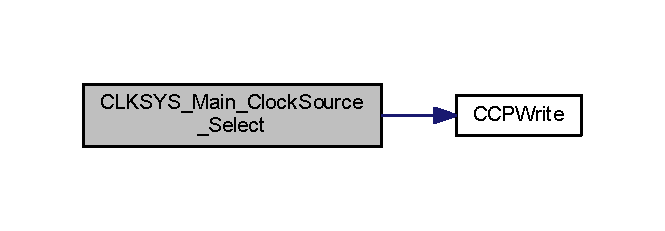
\includegraphics[width=319pt]{clksys__driver_8c_a1e46c4a8f01a83d4e4747d32d113e7e2_cgraph}
\end{center}
\end{figure}
Here is the caller graph for this function\+:\nopagebreak
\begin{figure}[H]
\begin{center}
\leavevmode
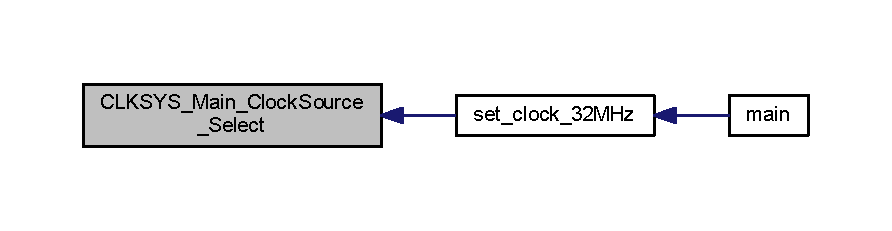
\includegraphics[width=350pt]{clksys__driver_8c_a1e46c4a8f01a83d4e4747d32d113e7e2_icgraph}
\end{center}
\end{figure}
\hypertarget{clksys__driver_8c_acb82744003806825da7fb6a7bb973941}{}\label{clksys__driver_8c_acb82744003806825da7fb6a7bb973941} 
\index{clksys\+\_\+driver.\+c@{clksys\+\_\+driver.\+c}!C\+L\+K\+S\+Y\+S\+\_\+\+P\+L\+L\+\_\+\+Config@{C\+L\+K\+S\+Y\+S\+\_\+\+P\+L\+L\+\_\+\+Config}}
\index{C\+L\+K\+S\+Y\+S\+\_\+\+P\+L\+L\+\_\+\+Config@{C\+L\+K\+S\+Y\+S\+\_\+\+P\+L\+L\+\_\+\+Config}!clksys\+\_\+driver.\+c@{clksys\+\_\+driver.\+c}}
\subsubsection{\texorpdfstring{C\+L\+K\+S\+Y\+S\+\_\+\+P\+L\+L\+\_\+\+Config()}{CLKSYS\_PLL\_Config()}}
{\footnotesize\ttfamily void C\+L\+K\+S\+Y\+S\+\_\+\+P\+L\+L\+\_\+\+Config (\begin{DoxyParamCaption}\item[{O\+S\+C\+\_\+\+P\+L\+L\+S\+R\+C\+\_\+t}]{clock\+Source,  }\item[{uint8\+\_\+t}]{factor }\end{DoxyParamCaption})}



This function configures the internal high-\/frequency P\+LL. 

Configuration of the internal high-\/frequency P\+LL to the correct values. It is used to define the input of the P\+LL and the factor of multiplication of the input clock source.

\begin{DoxyNote}{Note}
Note that the oscillator cannot be used as a main system clock source without being enabled and stable first. Check the ready flag before using the clock. The macro \hyperlink{clksys__driver_8h_a2cd92dbb89e4051b9385a61273d19dc6}{C\+L\+K\+S\+Y\+S\+\_\+\+Is\+Ready( \+\_\+osc\+Sel )} can be used to check this.
\end{DoxyNote}

\begin{DoxyParams}{Parameters}
{\em clock\+Source} & Reference clock source for the P\+LL, must be above 0.\+4\+M\+Hz. \\
\hline
{\em factor} & P\+LL multiplication factor, must be from 1 to 31, inclusive. \\
\hline
\end{DoxyParams}


Definition at line 167 of file clksys\+\_\+driver.\+c.

\hypertarget{clksys__driver_8c_a8e350b689dc409a4c9b902a192d1e8a3}{}\label{clksys__driver_8c_a8e350b689dc409a4c9b902a192d1e8a3} 
\index{clksys\+\_\+driver.\+c@{clksys\+\_\+driver.\+c}!C\+L\+K\+S\+Y\+S\+\_\+\+Prescalers\+\_\+\+Config@{C\+L\+K\+S\+Y\+S\+\_\+\+Prescalers\+\_\+\+Config}}
\index{C\+L\+K\+S\+Y\+S\+\_\+\+Prescalers\+\_\+\+Config@{C\+L\+K\+S\+Y\+S\+\_\+\+Prescalers\+\_\+\+Config}!clksys\+\_\+driver.\+c@{clksys\+\_\+driver.\+c}}
\subsubsection{\texorpdfstring{C\+L\+K\+S\+Y\+S\+\_\+\+Prescalers\+\_\+\+Config()}{CLKSYS\_Prescalers\_Config()}}
{\footnotesize\ttfamily void C\+L\+K\+S\+Y\+S\+\_\+\+Prescalers\+\_\+\+Config (\begin{DoxyParamCaption}\item[{C\+L\+K\+\_\+\+P\+S\+A\+D\+I\+V\+\_\+t}]{P\+S\+Afactor,  }\item[{C\+L\+K\+\_\+\+P\+S\+B\+C\+D\+I\+V\+\_\+t}]{P\+S\+B\+Cfactor }\end{DoxyParamCaption})}



This function changes the prescaler configuration. 

Change the configuration of the three system clock prescaler is one single operation. The user must make sure that the main C\+PU clock does not exceed recommended limits.


\begin{DoxyParams}{Parameters}
{\em P\+S\+Afactor} & Prescaler A division factor, O\+FF or 2 to 512 in powers of two. \\
\hline
{\em P\+S\+B\+Cfactor} & Prescaler B and C division factor, in the combination of (1,1), (1,2), (4,1) or (2,2). \\
\hline
\end{DoxyParams}


Definition at line 206 of file clksys\+\_\+driver.\+c.



References C\+C\+P\+Write().

Here is the call graph for this function\+:\nopagebreak
\begin{figure}[H]
\begin{center}
\leavevmode
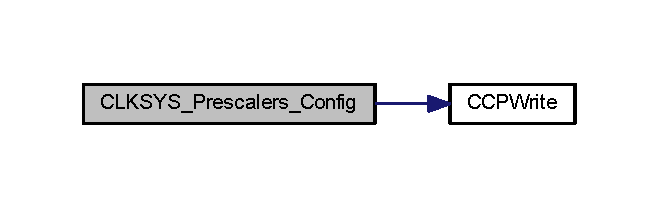
\includegraphics[width=316pt]{clksys__driver_8c_a8e350b689dc409a4c9b902a192d1e8a3_cgraph}
\end{center}
\end{figure}
\hypertarget{clksys__driver_8c_ae622e3056cd713fdca464b9fd6e5a7ab}{}\label{clksys__driver_8c_ae622e3056cd713fdca464b9fd6e5a7ab} 
\index{clksys\+\_\+driver.\+c@{clksys\+\_\+driver.\+c}!C\+L\+K\+S\+Y\+S\+\_\+\+R\+T\+C\+\_\+\+Clock\+Source\+\_\+\+Enable@{C\+L\+K\+S\+Y\+S\+\_\+\+R\+T\+C\+\_\+\+Clock\+Source\+\_\+\+Enable}}
\index{C\+L\+K\+S\+Y\+S\+\_\+\+R\+T\+C\+\_\+\+Clock\+Source\+\_\+\+Enable@{C\+L\+K\+S\+Y\+S\+\_\+\+R\+T\+C\+\_\+\+Clock\+Source\+\_\+\+Enable}!clksys\+\_\+driver.\+c@{clksys\+\_\+driver.\+c}}
\subsubsection{\texorpdfstring{C\+L\+K\+S\+Y\+S\+\_\+\+R\+T\+C\+\_\+\+Clock\+Source\+\_\+\+Enable()}{CLKSYS\_RTC\_ClockSource\_Enable()}}
{\footnotesize\ttfamily void C\+L\+K\+S\+Y\+S\+\_\+\+R\+T\+C\+\_\+\+Clock\+Source\+\_\+\+Enable (\begin{DoxyParamCaption}\item[{C\+L\+K\+\_\+\+R\+T\+C\+S\+R\+C\+\_\+t}]{clock\+Source }\end{DoxyParamCaption})}



This function selects a Real-\/\+Time Counter clock source. 

Selects the clock source for use by the Real-\/\+Time Counter (R\+TC) and enables clock signal routing to the R\+TC module.


\begin{DoxyParams}{Parameters}
{\em clock\+Source} & Clock source to use for the R\+TC. \\
\hline
\end{DoxyParams}


Definition at line 241 of file clksys\+\_\+driver.\+c.

\hypertarget{clksys__driver_8c_ace371b352e90117520436eb125aeeec0}{}\label{clksys__driver_8c_ace371b352e90117520436eb125aeeec0} 
\index{clksys\+\_\+driver.\+c@{clksys\+\_\+driver.\+c}!C\+L\+K\+S\+Y\+S\+\_\+\+X\+O\+S\+C\+\_\+\+Config@{C\+L\+K\+S\+Y\+S\+\_\+\+X\+O\+S\+C\+\_\+\+Config}}
\index{C\+L\+K\+S\+Y\+S\+\_\+\+X\+O\+S\+C\+\_\+\+Config@{C\+L\+K\+S\+Y\+S\+\_\+\+X\+O\+S\+C\+\_\+\+Config}!clksys\+\_\+driver.\+c@{clksys\+\_\+driver.\+c}}
\subsubsection{\texorpdfstring{C\+L\+K\+S\+Y\+S\+\_\+\+X\+O\+S\+C\+\_\+\+Config()}{CLKSYS\_XOSC\_Config()}}
{\footnotesize\ttfamily void C\+L\+K\+S\+Y\+S\+\_\+\+X\+O\+S\+C\+\_\+\+Config (\begin{DoxyParamCaption}\item[{O\+S\+C\+\_\+\+F\+R\+Q\+R\+A\+N\+G\+E\+\_\+t}]{freq\+Range,  }\item[{bool}]{low\+Power32k\+Hz,  }\item[{O\+S\+C\+\_\+\+X\+O\+S\+C\+S\+E\+L\+\_\+t}]{xosc\+Mode\+Selection }\end{DoxyParamCaption})}



This function configures the external oscillator. 

\begin{DoxyNote}{Note}
Note that the oscillator cannot be used as a main system clock source without being enabled and stable first. Check the ready flag before using the clock. The macro \hyperlink{clksys__driver_8h_a2cd92dbb89e4051b9385a61273d19dc6}{C\+L\+K\+S\+Y\+S\+\_\+\+Is\+Ready( \+\_\+osc\+Sel )} can be used to check this.
\end{DoxyNote}

\begin{DoxyParams}{Parameters}
{\em freq\+Range} & Frequency range for high-\/frequency crystal, does not apply for external clock or 32k\+Hz crystals. \\
\hline
{\em low\+Power32k\+Hz} & True of high-\/quality watch crystals are used and low-\/power oscillator is desired. \\
\hline
{\em xosc\+Mode\+Selection} & Combined selection of oscillator type (or external clock) and startup times. \\
\hline
\end{DoxyParams}


Definition at line 141 of file clksys\+\_\+driver.\+c.

\hypertarget{clksys__driver_8c_abfb0da2d81736412af825d46e7e0cedb}{}\label{clksys__driver_8c_abfb0da2d81736412af825d46e7e0cedb} 
\index{clksys\+\_\+driver.\+c@{clksys\+\_\+driver.\+c}!C\+L\+K\+S\+Y\+S\+\_\+\+X\+O\+S\+C\+\_\+\+Failure\+Detection\+\_\+\+Enable@{C\+L\+K\+S\+Y\+S\+\_\+\+X\+O\+S\+C\+\_\+\+Failure\+Detection\+\_\+\+Enable}}
\index{C\+L\+K\+S\+Y\+S\+\_\+\+X\+O\+S\+C\+\_\+\+Failure\+Detection\+\_\+\+Enable@{C\+L\+K\+S\+Y\+S\+\_\+\+X\+O\+S\+C\+\_\+\+Failure\+Detection\+\_\+\+Enable}!clksys\+\_\+driver.\+c@{clksys\+\_\+driver.\+c}}
\subsubsection{\texorpdfstring{C\+L\+K\+S\+Y\+S\+\_\+\+X\+O\+S\+C\+\_\+\+Failure\+Detection\+\_\+\+Enable()}{CLKSYS\_XOSC\_FailureDetection\_Enable()}}
{\footnotesize\ttfamily void C\+L\+K\+S\+Y\+S\+\_\+\+X\+O\+S\+C\+\_\+\+Failure\+Detection\+\_\+\+Enable (\begin{DoxyParamCaption}\item[{void}]{ }\end{DoxyParamCaption})}



This function enables the External Oscillator Failure Detection (X\+O\+S\+C\+FD) feature. 

The feature will stay enabled until next reset. Note that the X\+O\+S\+C\+FD {\itshape will} issue the X\+O\+S\+CF Non-\/maskable Interrupt (N\+MI) regardless of any interrupt priorities and settings. Therefore, make sure that a handler is implemented for the X\+O\+S\+CF N\+MI when you enable it. 

Definition at line 280 of file clksys\+\_\+driver.\+c.



References C\+C\+P\+Write().

Here is the call graph for this function\+:\nopagebreak
\begin{figure}[H]
\begin{center}
\leavevmode
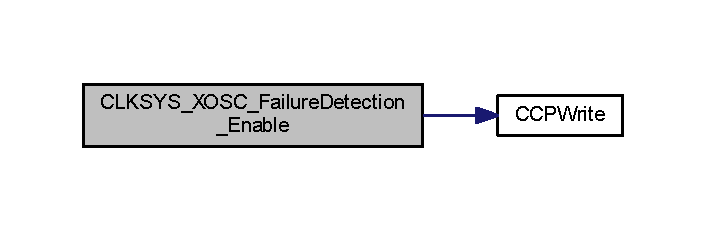
\includegraphics[width=339pt]{clksys__driver_8c_abfb0da2d81736412af825d46e7e0cedb_cgraph}
\end{center}
\end{figure}

\hypertarget{clksys__driver_8h}{}\section{clksys\+\_\+driver.\+h File Reference}
\label{clksys__driver_8h}\index{clksys\+\_\+driver.\+h@{clksys\+\_\+driver.\+h}}


X\+M\+E\+GA Clock System driver header file.  


{\ttfamily \#include \char`\"{}avr\+\_\+compiler.\+h\char`\"{}}\newline
Include dependency graph for clksys\+\_\+driver.\+h\+:\nopagebreak
\begin{figure}[H]
\begin{center}
\leavevmode
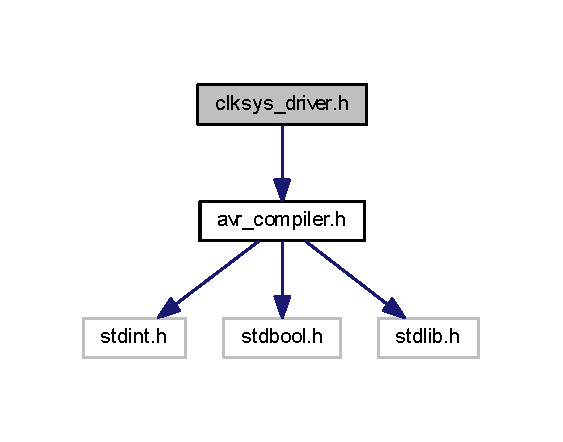
\includegraphics[width=270pt]{clksys__driver_8h__incl}
\end{center}
\end{figure}
This graph shows which files directly or indirectly include this file\+:\nopagebreak
\begin{figure}[H]
\begin{center}
\leavevmode
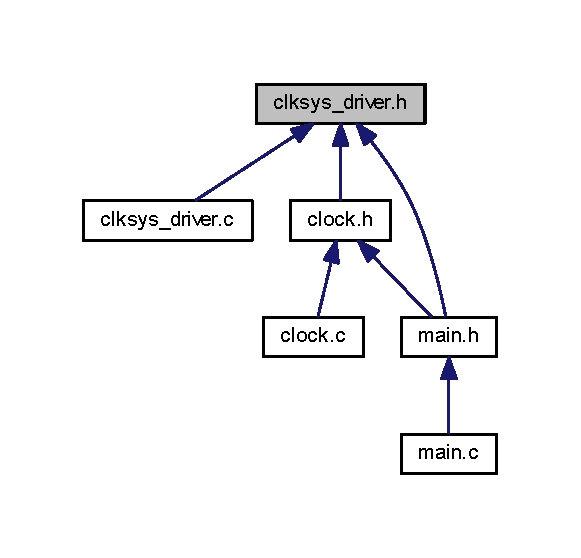
\includegraphics[width=279pt]{clksys__driver_8h__dep__incl}
\end{center}
\end{figure}
\subsection*{Macros}
\begin{DoxyCompactItemize}
\item 
\#define \hyperlink{clksys__driver_8h_a0894c64562c3b1c309bab97a83382267}{C\+L\+K\+S\+Y\+S\+\_\+\+Enable}(\+\_\+osc\+Sel)~( O\+S\+C.\+C\+T\+RL $\vert$= (\+\_\+osc\+Sel) )
\begin{DoxyCompactList}\small\item\em This macro enables the selected oscillator. \end{DoxyCompactList}\item 
\#define \hyperlink{clksys__driver_8h_a2cd92dbb89e4051b9385a61273d19dc6}{C\+L\+K\+S\+Y\+S\+\_\+\+Is\+Ready}(\+\_\+osc\+Sel)~( O\+S\+C.\+S\+T\+A\+T\+US \& (\+\_\+osc\+Sel) )
\begin{DoxyCompactList}\small\item\em This macro check if selected oscillator is ready. \end{DoxyCompactList}\item 
\#define \hyperlink{clksys__driver_8h_a2ace04e605910a306c6f65102e76c046}{C\+L\+K\+S\+Y\+S\+\_\+\+R\+T\+C\+\_\+\+Clock\+Source\+\_\+\+Disable}()~( C\+L\+K.\+R\+T\+C\+C\+T\+RL \&= $\sim$C\+L\+K\+\_\+\+R\+T\+C\+E\+N\+\_\+bm )
\begin{DoxyCompactList}\small\item\em This macro disables routing of clock signals to the Real-\/\+Time Counter (R\+TC). \end{DoxyCompactList}\item 
\#define \hyperlink{clksys__driver_8h_ab06829d3775b72351cbb2cb65dbc4dc7}{C\+L\+K\+S\+Y\+S\+\_\+\+Auto\+Calibration\+\_\+\+Disable}(\+\_\+clk)~( (\+\_\+clk).C\+T\+RL \&= $\sim$D\+F\+L\+L\+\_\+\+E\+N\+A\+B\+L\+E\+\_\+bm )
\begin{DoxyCompactList}\small\item\em This macro disables the automatic calibration of the selected internal oscillator. \end{DoxyCompactList}\end{DoxyCompactItemize}
\subsection*{Functions}
\begin{DoxyCompactItemize}
\item 
void \hyperlink{clksys__driver_8h_aad4e162434c2cc7e0087bbc0ddfe266c}{C\+C\+P\+Write} (volatile uint8\+\_\+t $\ast$address, uint8\+\_\+t value)
\begin{DoxyCompactList}\small\item\em C\+CP write helper function written in assembly. \end{DoxyCompactList}\item 
void \hyperlink{clksys__driver_8h_ace371b352e90117520436eb125aeeec0}{C\+L\+K\+S\+Y\+S\+\_\+\+X\+O\+S\+C\+\_\+\+Config} (O\+S\+C\+\_\+\+F\+R\+Q\+R\+A\+N\+G\+E\+\_\+t freq\+Range, bool low\+Power32k\+Hz, O\+S\+C\+\_\+\+X\+O\+S\+C\+S\+E\+L\+\_\+t xosc\+Mode\+Selection)
\begin{DoxyCompactList}\small\item\em This function configures the external oscillator. \end{DoxyCompactList}\item 
void \hyperlink{clksys__driver_8h_acb82744003806825da7fb6a7bb973941}{C\+L\+K\+S\+Y\+S\+\_\+\+P\+L\+L\+\_\+\+Config} (O\+S\+C\+\_\+\+P\+L\+L\+S\+R\+C\+\_\+t clock\+Source, uint8\+\_\+t factor)
\begin{DoxyCompactList}\small\item\em This function configures the internal high-\/frequency P\+LL. \end{DoxyCompactList}\item 
uint8\+\_\+t \hyperlink{clksys__driver_8h_a31b1ca1994b6a687974a119d1ad8008c}{C\+L\+K\+S\+Y\+S\+\_\+\+Disable} (uint8\+\_\+t osc\+Sel)
\begin{DoxyCompactList}\small\item\em This function disables the selected oscillator. \end{DoxyCompactList}\item 
void \hyperlink{clksys__driver_8h_a8e350b689dc409a4c9b902a192d1e8a3}{C\+L\+K\+S\+Y\+S\+\_\+\+Prescalers\+\_\+\+Config} (C\+L\+K\+\_\+\+P\+S\+A\+D\+I\+V\+\_\+t P\+S\+Afactor, C\+L\+K\+\_\+\+P\+S\+B\+C\+D\+I\+V\+\_\+t P\+S\+B\+Cfactor)
\begin{DoxyCompactList}\small\item\em This function changes the prescaler configuration. \end{DoxyCompactList}\item 
uint8\+\_\+t \hyperlink{clksys__driver_8h_a1e46c4a8f01a83d4e4747d32d113e7e2}{C\+L\+K\+S\+Y\+S\+\_\+\+Main\+\_\+\+Clock\+Source\+\_\+\+Select} (C\+L\+K\+\_\+\+S\+C\+L\+K\+S\+E\+L\+\_\+t clock\+Source)
\begin{DoxyCompactList}\small\item\em This function selects the main system clock source. \end{DoxyCompactList}\item 
void \hyperlink{clksys__driver_8h_ae622e3056cd713fdca464b9fd6e5a7ab}{C\+L\+K\+S\+Y\+S\+\_\+\+R\+T\+C\+\_\+\+Clock\+Source\+\_\+\+Enable} (C\+L\+K\+\_\+\+R\+T\+C\+S\+R\+C\+\_\+t clock\+Source)
\begin{DoxyCompactList}\small\item\em This function selects a Real-\/\+Time Counter clock source. \end{DoxyCompactList}\item 
void \hyperlink{clksys__driver_8h_a581c15c6c0b2eaa0c81f0b5cafc3b82d}{C\+L\+K\+S\+Y\+S\+\_\+\+Auto\+Calibration\+\_\+\+Enable} (uint8\+\_\+t clk\+Source, bool ext\+Reference)
\begin{DoxyCompactList}\small\item\em This function enables automatic calibration of the selected internal oscillator. \end{DoxyCompactList}\item 
void \hyperlink{clksys__driver_8h_abfb0da2d81736412af825d46e7e0cedb}{C\+L\+K\+S\+Y\+S\+\_\+\+X\+O\+S\+C\+\_\+\+Failure\+Detection\+\_\+\+Enable} (void)
\begin{DoxyCompactList}\small\item\em This function enables the External Oscillator Failure Detection (X\+O\+S\+C\+FD) feature. \end{DoxyCompactList}\item 
void \hyperlink{clksys__driver_8h_a6225fea8fc405c6d1dab88d0ad537173}{C\+L\+K\+S\+Y\+S\+\_\+\+Configuration\+\_\+\+Lock} (void)
\begin{DoxyCompactList}\small\item\em This function lock the entire clock system configuration. \end{DoxyCompactList}\end{DoxyCompactItemize}


\subsection{Detailed Description}
X\+M\+E\+GA Clock System driver header file. 

This file contains the function prototypes and enumerator definitions for various configuration parameters for the X\+M\+E\+GA Clock System driver.

The driver is not intended for size and/or speed critical code, since most functions are just a few lines of code, and the function call overhead would decrease code performance. The driver is intended for rapid prototyping and documentation purposes for getting started with the X\+M\+E\+GA Clock System.

For size and/or speed critical code, it is recommended to copy the function contents directly into your application instead of making a function call.

\begin{DoxyParagraph}{Application note\+:}
A\+V\+R1003\+: Using the X\+M\+E\+GA Clock System
\end{DoxyParagraph}
\begin{DoxyParagraph}{Documentation}
For comprehensive code documentation, supported compilers, compiler settings and supported devices see readme.\+html
\end{DoxyParagraph}
\begin{DoxyAuthor}{Author}
Atmel Corporation\+: \href{http://www.atmel.com}{\tt http\+://www.\+atmel.\+com} ~\newline
 Support email\+: \href{mailto:avr@atmel.com}{\tt avr@atmel.\+com}
\end{DoxyAuthor}
\begin{DoxyParagraph}{Revision}
1665 
\end{DoxyParagraph}
\begin{DoxyParagraph}{Date}
2008-\/06-\/05 09\+:21\+:50 +0200 (to, 05 jun 2008) 
\end{DoxyParagraph}
~\newline
 Copyright (c) 2008, Atmel Corporation All rights reserved.

Redistribution and use in source and binary forms, with or without modification, are permitted provided that the following conditions are met\+:


\begin{DoxyEnumerate}
\item Redistributions of source code must retain the above copyright notice, this list of conditions and the following disclaimer.
\item Redistributions in binary form must reproduce the above copyright notice, this list of conditions and the following disclaimer in the documentation and/or other materials provided with the distribution.
\item The name of A\+T\+M\+EL may not be used to endorse or promote products derived from this software without specific prior written permission.
\end{DoxyEnumerate}

T\+H\+IS S\+O\+F\+T\+W\+A\+RE IS P\+R\+O\+V\+I\+D\+ED BY A\+T\+M\+EL \char`\"{}\+A\+S I\+S\char`\"{} A\+ND A\+NY E\+X\+P\+R\+E\+SS OR I\+M\+P\+L\+I\+ED W\+A\+R\+R\+A\+N\+T\+I\+ES, I\+N\+C\+L\+U\+D\+I\+NG, B\+UT N\+OT L\+I\+M\+I\+T\+ED TO, T\+HE I\+M\+P\+L\+I\+ED W\+A\+R\+R\+A\+N\+T\+I\+ES OF M\+E\+R\+C\+H\+A\+N\+T\+A\+B\+I\+L\+I\+TY A\+ND F\+I\+T\+N\+E\+SS F\+OR A P\+A\+R\+T\+I\+C\+U\+L\+AR P\+U\+R\+P\+O\+SE A\+RE E\+X\+P\+R\+E\+S\+S\+LY A\+ND S\+P\+E\+C\+I\+F\+I\+C\+A\+L\+LY D\+I\+S\+C\+L\+A\+I\+M\+ED. IN NO E\+V\+E\+NT S\+H\+A\+LL A\+T\+M\+EL BE L\+I\+A\+B\+LE F\+OR A\+NY D\+I\+R\+E\+CT, I\+N\+D\+I\+R\+E\+CT, I\+N\+C\+I\+D\+E\+N\+T\+AL, S\+P\+E\+C\+I\+AL, E\+X\+E\+M\+P\+L\+A\+RY, OR C\+O\+N\+S\+E\+Q\+U\+E\+N\+T\+I\+AL D\+A\+M\+A\+G\+ES (I\+N\+C\+L\+U\+D\+I\+NG, B\+UT N\+OT L\+I\+M\+I\+T\+ED TO, P\+R\+O\+C\+U\+R\+E\+M\+E\+NT OF S\+U\+B\+S\+T\+I\+T\+U\+TE G\+O\+O\+DS OR S\+E\+R\+V\+I\+C\+ES; L\+O\+SS OF U\+SE, D\+A\+TA, OR P\+R\+O\+F\+I\+TS; OR B\+U\+S\+I\+N\+E\+SS I\+N\+T\+E\+R\+R\+U\+P\+T\+I\+ON) H\+O\+W\+E\+V\+ER C\+A\+U\+S\+ED A\+ND ON A\+NY T\+H\+E\+O\+RY OF L\+I\+A\+B\+I\+L\+I\+TY, W\+H\+E\+T\+H\+ER IN C\+O\+N\+T\+R\+A\+CT, S\+T\+R\+I\+CT L\+I\+A\+B\+I\+L\+I\+TY, OR T\+O\+RT (I\+N\+C\+L\+U\+D\+I\+NG N\+E\+G\+L\+I\+G\+E\+N\+CE OR O\+T\+H\+E\+R\+W\+I\+SE) A\+R\+I\+S\+I\+NG IN A\+NY W\+AY O\+UT OF T\+HE U\+SE OF T\+H\+IS S\+O\+F\+T\+W\+A\+RE, E\+V\+EN IF A\+D\+V\+I\+S\+ED OF T\+HE P\+O\+S\+S\+I\+B\+I\+L\+I\+TY OF S\+U\+CH D\+A\+M\+A\+GE. 

\subsection{Macro Definition Documentation}
\hypertarget{clksys__driver_8h_ab06829d3775b72351cbb2cb65dbc4dc7}{}\label{clksys__driver_8h_ab06829d3775b72351cbb2cb65dbc4dc7} 
\index{clksys\+\_\+driver.\+h@{clksys\+\_\+driver.\+h}!C\+L\+K\+S\+Y\+S\+\_\+\+Auto\+Calibration\+\_\+\+Disable@{C\+L\+K\+S\+Y\+S\+\_\+\+Auto\+Calibration\+\_\+\+Disable}}
\index{C\+L\+K\+S\+Y\+S\+\_\+\+Auto\+Calibration\+\_\+\+Disable@{C\+L\+K\+S\+Y\+S\+\_\+\+Auto\+Calibration\+\_\+\+Disable}!clksys\+\_\+driver.\+h@{clksys\+\_\+driver.\+h}}
\subsubsection{\texorpdfstring{C\+L\+K\+S\+Y\+S\+\_\+\+Auto\+Calibration\+\_\+\+Disable}{CLKSYS\_AutoCalibration\_Disable}}
{\footnotesize\ttfamily \#define C\+L\+K\+S\+Y\+S\+\_\+\+Auto\+Calibration\+\_\+\+Disable(\begin{DoxyParamCaption}\item[{}]{\+\_\+clk }\end{DoxyParamCaption})~( (\+\_\+clk).C\+T\+RL \&= $\sim$D\+F\+L\+L\+\_\+\+E\+N\+A\+B\+L\+E\+\_\+bm )}



This macro disables the automatic calibration of the selected internal oscillator. 


\begin{DoxyParams}{Parameters}
{\em \+\_\+clk} & Clock source calibration to disable, either D\+F\+L\+L\+R\+C2M or D\+F\+L\+L\+R\+C32M. \\
\hline
\end{DoxyParams}


Definition at line 105 of file clksys\+\_\+driver.\+h.

\hypertarget{clksys__driver_8h_a0894c64562c3b1c309bab97a83382267}{}\label{clksys__driver_8h_a0894c64562c3b1c309bab97a83382267} 
\index{clksys\+\_\+driver.\+h@{clksys\+\_\+driver.\+h}!C\+L\+K\+S\+Y\+S\+\_\+\+Enable@{C\+L\+K\+S\+Y\+S\+\_\+\+Enable}}
\index{C\+L\+K\+S\+Y\+S\+\_\+\+Enable@{C\+L\+K\+S\+Y\+S\+\_\+\+Enable}!clksys\+\_\+driver.\+h@{clksys\+\_\+driver.\+h}}
\subsubsection{\texorpdfstring{C\+L\+K\+S\+Y\+S\+\_\+\+Enable}{CLKSYS\_Enable}}
{\footnotesize\ttfamily \#define C\+L\+K\+S\+Y\+S\+\_\+\+Enable(\begin{DoxyParamCaption}\item[{}]{\+\_\+osc\+Sel }\end{DoxyParamCaption})~( O\+S\+C.\+C\+T\+RL $\vert$= (\+\_\+osc\+Sel) )}



This macro enables the selected oscillator. 

\begin{DoxyNote}{Note}
Note that the oscillator cannot be used as a main system clock source without being enabled and stable first. Check the ready flag before using the clock. The function \hyperlink{clksys__driver_8h_a2cd92dbb89e4051b9385a61273d19dc6}{C\+L\+K\+S\+Y\+S\+\_\+\+Is\+Ready( \+\_\+osc\+Sel )} can be used to check this.
\end{DoxyNote}

\begin{DoxyParams}{Parameters}
{\em \+\_\+osc\+Sel} & Bitmask of selected clock. Can be one of the following O\+S\+C\+\_\+\+R\+C2\+M\+E\+N\+\_\+bm, O\+S\+C\+\_\+\+R\+C32\+M\+E\+N\+\_\+bm, O\+S\+C\+\_\+\+R\+C32\+K\+E\+N\+\_\+bm, O\+S\+C\+\_\+\+X\+O\+S\+C\+E\+N\+\_\+bm, O\+S\+C\+\_\+\+P\+L\+L\+E\+N\+\_\+bm. \\
\hline
\end{DoxyParams}


Definition at line 78 of file clksys\+\_\+driver.\+h.



Referenced by set\+\_\+clock\+\_\+32\+M\+Hz().

\hypertarget{clksys__driver_8h_a2cd92dbb89e4051b9385a61273d19dc6}{}\label{clksys__driver_8h_a2cd92dbb89e4051b9385a61273d19dc6} 
\index{clksys\+\_\+driver.\+h@{clksys\+\_\+driver.\+h}!C\+L\+K\+S\+Y\+S\+\_\+\+Is\+Ready@{C\+L\+K\+S\+Y\+S\+\_\+\+Is\+Ready}}
\index{C\+L\+K\+S\+Y\+S\+\_\+\+Is\+Ready@{C\+L\+K\+S\+Y\+S\+\_\+\+Is\+Ready}!clksys\+\_\+driver.\+h@{clksys\+\_\+driver.\+h}}
\subsubsection{\texorpdfstring{C\+L\+K\+S\+Y\+S\+\_\+\+Is\+Ready}{CLKSYS\_IsReady}}
{\footnotesize\ttfamily \#define C\+L\+K\+S\+Y\+S\+\_\+\+Is\+Ready(\begin{DoxyParamCaption}\item[{}]{\+\_\+osc\+Sel }\end{DoxyParamCaption})~( O\+S\+C.\+S\+T\+A\+T\+US \& (\+\_\+osc\+Sel) )}



This macro check if selected oscillator is ready. 

This macro will return non-\/zero if is is running, regardless if it is used as a main clock source or not.


\begin{DoxyParams}{Parameters}
{\em \+\_\+osc\+Sel} & Bitmask of selected clock. Can be one of the following O\+S\+C\+\_\+\+R\+C2\+M\+E\+N\+\_\+bm, O\+S\+C\+\_\+\+R\+C32\+M\+E\+N\+\_\+bm, O\+S\+C\+\_\+\+R\+C32\+K\+E\+N\+\_\+bm, O\+S\+C\+\_\+\+X\+O\+S\+C\+E\+N\+\_\+bm, O\+S\+C\+\_\+\+P\+L\+L\+E\+N\+\_\+bm.\\
\hline
\end{DoxyParams}
\begin{DoxyReturn}{Returns}
Non-\/zero if oscillator is ready and running. 
\end{DoxyReturn}


Definition at line 91 of file clksys\+\_\+driver.\+h.



Referenced by set\+\_\+clock\+\_\+32\+M\+Hz().

\hypertarget{clksys__driver_8h_a2ace04e605910a306c6f65102e76c046}{}\label{clksys__driver_8h_a2ace04e605910a306c6f65102e76c046} 
\index{clksys\+\_\+driver.\+h@{clksys\+\_\+driver.\+h}!C\+L\+K\+S\+Y\+S\+\_\+\+R\+T\+C\+\_\+\+Clock\+Source\+\_\+\+Disable@{C\+L\+K\+S\+Y\+S\+\_\+\+R\+T\+C\+\_\+\+Clock\+Source\+\_\+\+Disable}}
\index{C\+L\+K\+S\+Y\+S\+\_\+\+R\+T\+C\+\_\+\+Clock\+Source\+\_\+\+Disable@{C\+L\+K\+S\+Y\+S\+\_\+\+R\+T\+C\+\_\+\+Clock\+Source\+\_\+\+Disable}!clksys\+\_\+driver.\+h@{clksys\+\_\+driver.\+h}}
\subsubsection{\texorpdfstring{C\+L\+K\+S\+Y\+S\+\_\+\+R\+T\+C\+\_\+\+Clock\+Source\+\_\+\+Disable}{CLKSYS\_RTC\_ClockSource\_Disable}}
{\footnotesize\ttfamily \#define C\+L\+K\+S\+Y\+S\+\_\+\+R\+T\+C\+\_\+\+Clock\+Source\+\_\+\+Disable(\begin{DoxyParamCaption}{ }\end{DoxyParamCaption})~( C\+L\+K.\+R\+T\+C\+C\+T\+RL \&= $\sim$C\+L\+K\+\_\+\+R\+T\+C\+E\+N\+\_\+bm )}



This macro disables routing of clock signals to the Real-\/\+Time Counter (R\+TC). 

Disabling the R\+TC saves power if the R\+TC is not in use. 

Definition at line 98 of file clksys\+\_\+driver.\+h.



\subsection{Function Documentation}
\hypertarget{clksys__driver_8h_aad4e162434c2cc7e0087bbc0ddfe266c}{}\label{clksys__driver_8h_aad4e162434c2cc7e0087bbc0ddfe266c} 
\index{clksys\+\_\+driver.\+h@{clksys\+\_\+driver.\+h}!C\+C\+P\+Write@{C\+C\+P\+Write}}
\index{C\+C\+P\+Write@{C\+C\+P\+Write}!clksys\+\_\+driver.\+h@{clksys\+\_\+driver.\+h}}
\subsubsection{\texorpdfstring{C\+C\+P\+Write()}{CCPWrite()}}
{\footnotesize\ttfamily void C\+C\+P\+Write (\begin{DoxyParamCaption}\item[{volatile uint8\+\_\+t $\ast$}]{address,  }\item[{uint8\+\_\+t}]{value }\end{DoxyParamCaption})}



C\+CP write helper function written in assembly. 

This function is written in assembly because of the timecritial operation of writing to the registers.


\begin{DoxyParams}{Parameters}
{\em address} & A pointer to the address to write to. \\
\hline
{\em value} & The value to put in to the register. \\
\hline
\end{DoxyParams}


Definition at line 77 of file clksys\+\_\+driver.\+c.



References A\+V\+R\+\_\+\+E\+N\+T\+E\+R\+\_\+\+C\+R\+I\+T\+I\+C\+A\+L\+\_\+\+R\+E\+G\+I\+ON, and A\+V\+R\+\_\+\+L\+E\+A\+V\+E\+\_\+\+C\+R\+I\+T\+I\+C\+A\+L\+\_\+\+R\+E\+G\+I\+ON.



Referenced by C\+L\+K\+S\+Y\+S\+\_\+\+Configuration\+\_\+\+Lock(), C\+L\+K\+S\+Y\+S\+\_\+\+Main\+\_\+\+Clock\+Source\+\_\+\+Select(), C\+L\+K\+S\+Y\+S\+\_\+\+Prescalers\+\_\+\+Config(), and C\+L\+K\+S\+Y\+S\+\_\+\+X\+O\+S\+C\+\_\+\+Failure\+Detection\+\_\+\+Enable().

Here is the caller graph for this function\+:\nopagebreak
\begin{figure}[H]
\begin{center}
\leavevmode
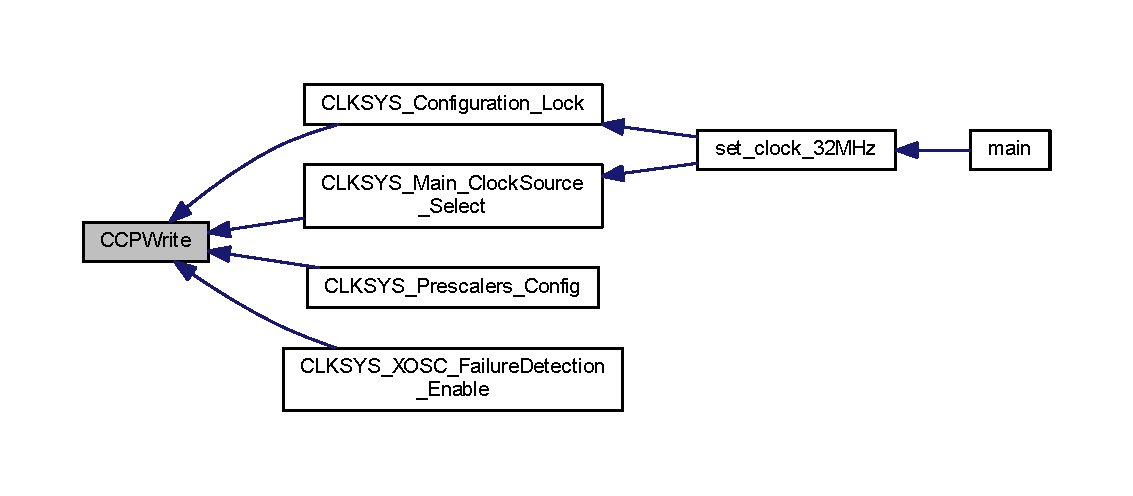
\includegraphics[width=350pt]{clksys__driver_8h_aad4e162434c2cc7e0087bbc0ddfe266c_icgraph}
\end{center}
\end{figure}
\hypertarget{clksys__driver_8h_a581c15c6c0b2eaa0c81f0b5cafc3b82d}{}\label{clksys__driver_8h_a581c15c6c0b2eaa0c81f0b5cafc3b82d} 
\index{clksys\+\_\+driver.\+h@{clksys\+\_\+driver.\+h}!C\+L\+K\+S\+Y\+S\+\_\+\+Auto\+Calibration\+\_\+\+Enable@{C\+L\+K\+S\+Y\+S\+\_\+\+Auto\+Calibration\+\_\+\+Enable}}
\index{C\+L\+K\+S\+Y\+S\+\_\+\+Auto\+Calibration\+\_\+\+Enable@{C\+L\+K\+S\+Y\+S\+\_\+\+Auto\+Calibration\+\_\+\+Enable}!clksys\+\_\+driver.\+h@{clksys\+\_\+driver.\+h}}
\subsubsection{\texorpdfstring{C\+L\+K\+S\+Y\+S\+\_\+\+Auto\+Calibration\+\_\+\+Enable()}{CLKSYS\_AutoCalibration\_Enable()}}
{\footnotesize\ttfamily void C\+L\+K\+S\+Y\+S\+\_\+\+Auto\+Calibration\+\_\+\+Enable (\begin{DoxyParamCaption}\item[{uint8\+\_\+t}]{clk\+Source,  }\item[{bool}]{ext\+Reference }\end{DoxyParamCaption})}



This function enables automatic calibration of the selected internal oscillator. 

Either the internal 32k\+Hz RC oscillator or an external 32k\+Hz crystal can be used as a calibration reference. The user must make sure that the selected reference is ready and running.


\begin{DoxyParams}{Parameters}
{\em clk\+Source} & Clock source to calibrate, either O\+S\+C\+\_\+\+R\+C2\+M\+C\+R\+E\+F\+\_\+bm or O\+S\+C\+\_\+\+R\+C32\+M\+C\+R\+E\+F\+\_\+gm -\/ patched to group mask(jb). \\
\hline
{\em ext\+Reference} & True if external crystal should be used as reference. \\
\hline
\end{DoxyParams}


Definition at line 260 of file clksys\+\_\+driver.\+c.



Referenced by set\+\_\+clock\+\_\+32\+M\+Hz().

Here is the caller graph for this function\+:\nopagebreak
\begin{figure}[H]
\begin{center}
\leavevmode
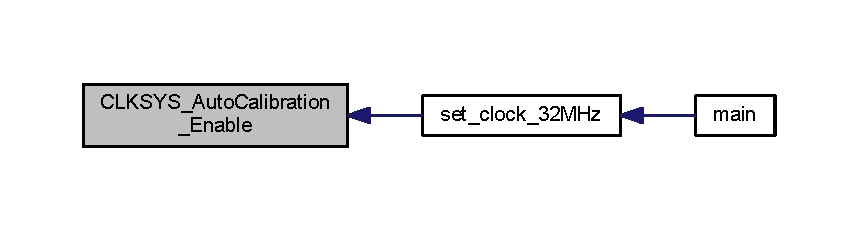
\includegraphics[width=350pt]{clksys__driver_8h_a581c15c6c0b2eaa0c81f0b5cafc3b82d_icgraph}
\end{center}
\end{figure}
\hypertarget{clksys__driver_8h_a6225fea8fc405c6d1dab88d0ad537173}{}\label{clksys__driver_8h_a6225fea8fc405c6d1dab88d0ad537173} 
\index{clksys\+\_\+driver.\+h@{clksys\+\_\+driver.\+h}!C\+L\+K\+S\+Y\+S\+\_\+\+Configuration\+\_\+\+Lock@{C\+L\+K\+S\+Y\+S\+\_\+\+Configuration\+\_\+\+Lock}}
\index{C\+L\+K\+S\+Y\+S\+\_\+\+Configuration\+\_\+\+Lock@{C\+L\+K\+S\+Y\+S\+\_\+\+Configuration\+\_\+\+Lock}!clksys\+\_\+driver.\+h@{clksys\+\_\+driver.\+h}}
\subsubsection{\texorpdfstring{C\+L\+K\+S\+Y\+S\+\_\+\+Configuration\+\_\+\+Lock()}{CLKSYS\_Configuration\_Lock()}}
{\footnotesize\ttfamily void C\+L\+K\+S\+Y\+S\+\_\+\+Configuration\+\_\+\+Lock (\begin{DoxyParamCaption}\item[{void}]{ }\end{DoxyParamCaption})}



This function lock the entire clock system configuration. 

This will lock the configuration until the next reset, or until the External Oscillator Failure Detections (X\+O\+S\+C\+FD) feature detects a failure and switches to internal 2\+M\+Hz RC oscillator. 

Definition at line 292 of file clksys\+\_\+driver.\+c.



References C\+C\+P\+Write().



Referenced by set\+\_\+clock\+\_\+32\+M\+Hz().

Here is the call graph for this function\+:\nopagebreak
\begin{figure}[H]
\begin{center}
\leavevmode
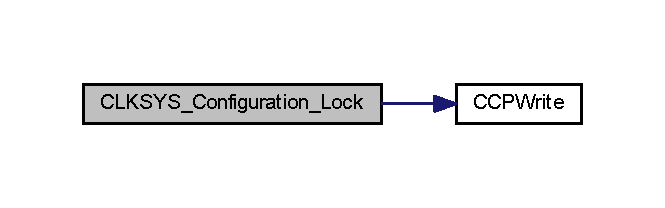
\includegraphics[width=319pt]{clksys__driver_8h_a6225fea8fc405c6d1dab88d0ad537173_cgraph}
\end{center}
\end{figure}
Here is the caller graph for this function\+:\nopagebreak
\begin{figure}[H]
\begin{center}
\leavevmode
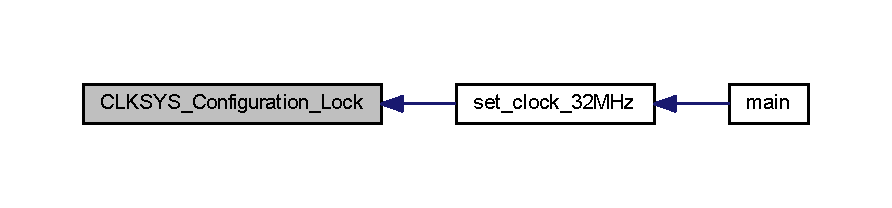
\includegraphics[width=350pt]{clksys__driver_8h_a6225fea8fc405c6d1dab88d0ad537173_icgraph}
\end{center}
\end{figure}
\hypertarget{clksys__driver_8h_a31b1ca1994b6a687974a119d1ad8008c}{}\label{clksys__driver_8h_a31b1ca1994b6a687974a119d1ad8008c} 
\index{clksys\+\_\+driver.\+h@{clksys\+\_\+driver.\+h}!C\+L\+K\+S\+Y\+S\+\_\+\+Disable@{C\+L\+K\+S\+Y\+S\+\_\+\+Disable}}
\index{C\+L\+K\+S\+Y\+S\+\_\+\+Disable@{C\+L\+K\+S\+Y\+S\+\_\+\+Disable}!clksys\+\_\+driver.\+h@{clksys\+\_\+driver.\+h}}
\subsubsection{\texorpdfstring{C\+L\+K\+S\+Y\+S\+\_\+\+Disable()}{CLKSYS\_Disable()}}
{\footnotesize\ttfamily uint8\+\_\+t C\+L\+K\+S\+Y\+S\+\_\+\+Disable (\begin{DoxyParamCaption}\item[{uint8\+\_\+t}]{osc\+Sel }\end{DoxyParamCaption})}



This function disables the selected oscillator. 

This function will disable the selected oscillator if possible. If it is currently used as a main system clock source, hardware will disregard the disable attempt, and this function will return zero. If it fails, change to another main system clock source and try again.


\begin{DoxyParams}{Parameters}
{\em osc\+Sel} & Bitmask of selected clock. Can be one of the following O\+S\+C\+\_\+\+R\+C2\+M\+E\+N\+\_\+bm, O\+S\+C\+\_\+\+R\+C32\+M\+E\+N\+\_\+bm, O\+S\+C\+\_\+\+R\+C32\+K\+E\+N\+\_\+bm, O\+S\+C\+\_\+\+X\+O\+S\+C\+E\+N\+\_\+bm, O\+S\+C\+\_\+\+P\+L\+L\+E\+N\+\_\+bm.\\
\hline
\end{DoxyParams}
\begin{DoxyReturn}{Returns}
Non-\/zero if oscillator was disabled successfully. 
\end{DoxyReturn}


Definition at line 187 of file clksys\+\_\+driver.\+c.



Referenced by set\+\_\+clock\+\_\+32\+M\+Hz().

Here is the caller graph for this function\+:\nopagebreak
\begin{figure}[H]
\begin{center}
\leavevmode
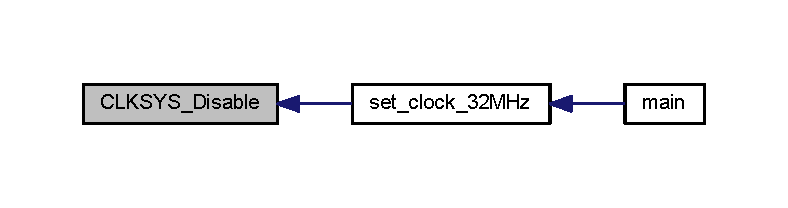
\includegraphics[width=350pt]{clksys__driver_8h_a31b1ca1994b6a687974a119d1ad8008c_icgraph}
\end{center}
\end{figure}
\hypertarget{clksys__driver_8h_a1e46c4a8f01a83d4e4747d32d113e7e2}{}\label{clksys__driver_8h_a1e46c4a8f01a83d4e4747d32d113e7e2} 
\index{clksys\+\_\+driver.\+h@{clksys\+\_\+driver.\+h}!C\+L\+K\+S\+Y\+S\+\_\+\+Main\+\_\+\+Clock\+Source\+\_\+\+Select@{C\+L\+K\+S\+Y\+S\+\_\+\+Main\+\_\+\+Clock\+Source\+\_\+\+Select}}
\index{C\+L\+K\+S\+Y\+S\+\_\+\+Main\+\_\+\+Clock\+Source\+\_\+\+Select@{C\+L\+K\+S\+Y\+S\+\_\+\+Main\+\_\+\+Clock\+Source\+\_\+\+Select}!clksys\+\_\+driver.\+h@{clksys\+\_\+driver.\+h}}
\subsubsection{\texorpdfstring{C\+L\+K\+S\+Y\+S\+\_\+\+Main\+\_\+\+Clock\+Source\+\_\+\+Select()}{CLKSYS\_Main\_ClockSource\_Select()}}
{\footnotesize\ttfamily uint8\+\_\+t C\+L\+K\+S\+Y\+S\+\_\+\+Main\+\_\+\+Clock\+Source\+\_\+\+Select (\begin{DoxyParamCaption}\item[{C\+L\+K\+\_\+\+S\+C\+L\+K\+S\+E\+L\+\_\+t}]{clock\+Source }\end{DoxyParamCaption})}



This function selects the main system clock source. 

Hardware will disregard any attempts to select a clock source that is not enabled or not stable. If the change fails, make sure the source is ready and running and try again.


\begin{DoxyParams}{Parameters}
{\em clock\+Source} & Clock source to use as input for the system clock prescaler block.\\
\hline
\end{DoxyParams}
\begin{DoxyReturn}{Returns}
Non-\/zero if change was successful. 
\end{DoxyReturn}


Definition at line 225 of file clksys\+\_\+driver.\+c.



References C\+C\+P\+Write().



Referenced by set\+\_\+clock\+\_\+32\+M\+Hz().

Here is the call graph for this function\+:\nopagebreak
\begin{figure}[H]
\begin{center}
\leavevmode
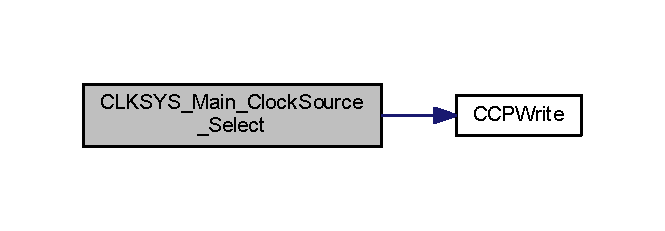
\includegraphics[width=319pt]{clksys__driver_8h_a1e46c4a8f01a83d4e4747d32d113e7e2_cgraph}
\end{center}
\end{figure}
Here is the caller graph for this function\+:\nopagebreak
\begin{figure}[H]
\begin{center}
\leavevmode
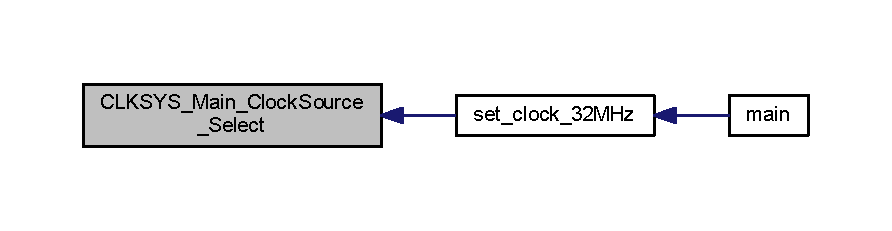
\includegraphics[width=350pt]{clksys__driver_8h_a1e46c4a8f01a83d4e4747d32d113e7e2_icgraph}
\end{center}
\end{figure}
\hypertarget{clksys__driver_8h_acb82744003806825da7fb6a7bb973941}{}\label{clksys__driver_8h_acb82744003806825da7fb6a7bb973941} 
\index{clksys\+\_\+driver.\+h@{clksys\+\_\+driver.\+h}!C\+L\+K\+S\+Y\+S\+\_\+\+P\+L\+L\+\_\+\+Config@{C\+L\+K\+S\+Y\+S\+\_\+\+P\+L\+L\+\_\+\+Config}}
\index{C\+L\+K\+S\+Y\+S\+\_\+\+P\+L\+L\+\_\+\+Config@{C\+L\+K\+S\+Y\+S\+\_\+\+P\+L\+L\+\_\+\+Config}!clksys\+\_\+driver.\+h@{clksys\+\_\+driver.\+h}}
\subsubsection{\texorpdfstring{C\+L\+K\+S\+Y\+S\+\_\+\+P\+L\+L\+\_\+\+Config()}{CLKSYS\_PLL\_Config()}}
{\footnotesize\ttfamily void C\+L\+K\+S\+Y\+S\+\_\+\+P\+L\+L\+\_\+\+Config (\begin{DoxyParamCaption}\item[{O\+S\+C\+\_\+\+P\+L\+L\+S\+R\+C\+\_\+t}]{clock\+Source,  }\item[{uint8\+\_\+t}]{factor }\end{DoxyParamCaption})}



This function configures the internal high-\/frequency P\+LL. 

Configuration of the internal high-\/frequency P\+LL to the correct values. It is used to define the input of the P\+LL and the factor of multiplication of the input clock source.

\begin{DoxyNote}{Note}
Note that the oscillator cannot be used as a main system clock source without being enabled and stable first. Check the ready flag before using the clock. The macro \hyperlink{clksys__driver_8h_a2cd92dbb89e4051b9385a61273d19dc6}{C\+L\+K\+S\+Y\+S\+\_\+\+Is\+Ready( \+\_\+osc\+Sel )} can be used to check this.
\end{DoxyNote}

\begin{DoxyParams}{Parameters}
{\em clock\+Source} & Reference clock source for the P\+LL, must be above 0.\+4\+M\+Hz. \\
\hline
{\em factor} & P\+LL multiplication factor, must be from 1 to 31, inclusive. \\
\hline
\end{DoxyParams}


Definition at line 167 of file clksys\+\_\+driver.\+c.

\hypertarget{clksys__driver_8h_a8e350b689dc409a4c9b902a192d1e8a3}{}\label{clksys__driver_8h_a8e350b689dc409a4c9b902a192d1e8a3} 
\index{clksys\+\_\+driver.\+h@{clksys\+\_\+driver.\+h}!C\+L\+K\+S\+Y\+S\+\_\+\+Prescalers\+\_\+\+Config@{C\+L\+K\+S\+Y\+S\+\_\+\+Prescalers\+\_\+\+Config}}
\index{C\+L\+K\+S\+Y\+S\+\_\+\+Prescalers\+\_\+\+Config@{C\+L\+K\+S\+Y\+S\+\_\+\+Prescalers\+\_\+\+Config}!clksys\+\_\+driver.\+h@{clksys\+\_\+driver.\+h}}
\subsubsection{\texorpdfstring{C\+L\+K\+S\+Y\+S\+\_\+\+Prescalers\+\_\+\+Config()}{CLKSYS\_Prescalers\_Config()}}
{\footnotesize\ttfamily void C\+L\+K\+S\+Y\+S\+\_\+\+Prescalers\+\_\+\+Config (\begin{DoxyParamCaption}\item[{C\+L\+K\+\_\+\+P\+S\+A\+D\+I\+V\+\_\+t}]{P\+S\+Afactor,  }\item[{C\+L\+K\+\_\+\+P\+S\+B\+C\+D\+I\+V\+\_\+t}]{P\+S\+B\+Cfactor }\end{DoxyParamCaption})}



This function changes the prescaler configuration. 

Change the configuration of the three system clock prescaler is one single operation. The user must make sure that the main C\+PU clock does not exceed recommended limits.


\begin{DoxyParams}{Parameters}
{\em P\+S\+Afactor} & Prescaler A division factor, O\+FF or 2 to 512 in powers of two. \\
\hline
{\em P\+S\+B\+Cfactor} & Prescaler B and C division factor, in the combination of (1,1), (1,2), (4,1) or (2,2). \\
\hline
\end{DoxyParams}


Definition at line 206 of file clksys\+\_\+driver.\+c.



References C\+C\+P\+Write().

Here is the call graph for this function\+:\nopagebreak
\begin{figure}[H]
\begin{center}
\leavevmode
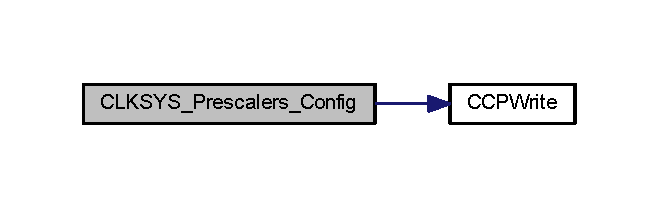
\includegraphics[width=316pt]{clksys__driver_8h_a8e350b689dc409a4c9b902a192d1e8a3_cgraph}
\end{center}
\end{figure}
\hypertarget{clksys__driver_8h_ae622e3056cd713fdca464b9fd6e5a7ab}{}\label{clksys__driver_8h_ae622e3056cd713fdca464b9fd6e5a7ab} 
\index{clksys\+\_\+driver.\+h@{clksys\+\_\+driver.\+h}!C\+L\+K\+S\+Y\+S\+\_\+\+R\+T\+C\+\_\+\+Clock\+Source\+\_\+\+Enable@{C\+L\+K\+S\+Y\+S\+\_\+\+R\+T\+C\+\_\+\+Clock\+Source\+\_\+\+Enable}}
\index{C\+L\+K\+S\+Y\+S\+\_\+\+R\+T\+C\+\_\+\+Clock\+Source\+\_\+\+Enable@{C\+L\+K\+S\+Y\+S\+\_\+\+R\+T\+C\+\_\+\+Clock\+Source\+\_\+\+Enable}!clksys\+\_\+driver.\+h@{clksys\+\_\+driver.\+h}}
\subsubsection{\texorpdfstring{C\+L\+K\+S\+Y\+S\+\_\+\+R\+T\+C\+\_\+\+Clock\+Source\+\_\+\+Enable()}{CLKSYS\_RTC\_ClockSource\_Enable()}}
{\footnotesize\ttfamily void C\+L\+K\+S\+Y\+S\+\_\+\+R\+T\+C\+\_\+\+Clock\+Source\+\_\+\+Enable (\begin{DoxyParamCaption}\item[{C\+L\+K\+\_\+\+R\+T\+C\+S\+R\+C\+\_\+t}]{clock\+Source }\end{DoxyParamCaption})}



This function selects a Real-\/\+Time Counter clock source. 

Selects the clock source for use by the Real-\/\+Time Counter (R\+TC) and enables clock signal routing to the R\+TC module.


\begin{DoxyParams}{Parameters}
{\em clock\+Source} & Clock source to use for the R\+TC. \\
\hline
\end{DoxyParams}


Definition at line 241 of file clksys\+\_\+driver.\+c.

\hypertarget{clksys__driver_8h_ace371b352e90117520436eb125aeeec0}{}\label{clksys__driver_8h_ace371b352e90117520436eb125aeeec0} 
\index{clksys\+\_\+driver.\+h@{clksys\+\_\+driver.\+h}!C\+L\+K\+S\+Y\+S\+\_\+\+X\+O\+S\+C\+\_\+\+Config@{C\+L\+K\+S\+Y\+S\+\_\+\+X\+O\+S\+C\+\_\+\+Config}}
\index{C\+L\+K\+S\+Y\+S\+\_\+\+X\+O\+S\+C\+\_\+\+Config@{C\+L\+K\+S\+Y\+S\+\_\+\+X\+O\+S\+C\+\_\+\+Config}!clksys\+\_\+driver.\+h@{clksys\+\_\+driver.\+h}}
\subsubsection{\texorpdfstring{C\+L\+K\+S\+Y\+S\+\_\+\+X\+O\+S\+C\+\_\+\+Config()}{CLKSYS\_XOSC\_Config()}}
{\footnotesize\ttfamily void C\+L\+K\+S\+Y\+S\+\_\+\+X\+O\+S\+C\+\_\+\+Config (\begin{DoxyParamCaption}\item[{O\+S\+C\+\_\+\+F\+R\+Q\+R\+A\+N\+G\+E\+\_\+t}]{freq\+Range,  }\item[{bool}]{low\+Power32k\+Hz,  }\item[{O\+S\+C\+\_\+\+X\+O\+S\+C\+S\+E\+L\+\_\+t}]{xosc\+Mode\+Selection }\end{DoxyParamCaption})}



This function configures the external oscillator. 

\begin{DoxyNote}{Note}
Note that the oscillator cannot be used as a main system clock source without being enabled and stable first. Check the ready flag before using the clock. The macro \hyperlink{clksys__driver_8h_a2cd92dbb89e4051b9385a61273d19dc6}{C\+L\+K\+S\+Y\+S\+\_\+\+Is\+Ready( \+\_\+osc\+Sel )} can be used to check this.
\end{DoxyNote}

\begin{DoxyParams}{Parameters}
{\em freq\+Range} & Frequency range for high-\/frequency crystal, does not apply for external clock or 32k\+Hz crystals. \\
\hline
{\em low\+Power32k\+Hz} & True of high-\/quality watch crystals are used and low-\/power oscillator is desired. \\
\hline
{\em xosc\+Mode\+Selection} & Combined selection of oscillator type (or external clock) and startup times. \\
\hline
\end{DoxyParams}


Definition at line 141 of file clksys\+\_\+driver.\+c.

\hypertarget{clksys__driver_8h_abfb0da2d81736412af825d46e7e0cedb}{}\label{clksys__driver_8h_abfb0da2d81736412af825d46e7e0cedb} 
\index{clksys\+\_\+driver.\+h@{clksys\+\_\+driver.\+h}!C\+L\+K\+S\+Y\+S\+\_\+\+X\+O\+S\+C\+\_\+\+Failure\+Detection\+\_\+\+Enable@{C\+L\+K\+S\+Y\+S\+\_\+\+X\+O\+S\+C\+\_\+\+Failure\+Detection\+\_\+\+Enable}}
\index{C\+L\+K\+S\+Y\+S\+\_\+\+X\+O\+S\+C\+\_\+\+Failure\+Detection\+\_\+\+Enable@{C\+L\+K\+S\+Y\+S\+\_\+\+X\+O\+S\+C\+\_\+\+Failure\+Detection\+\_\+\+Enable}!clksys\+\_\+driver.\+h@{clksys\+\_\+driver.\+h}}
\subsubsection{\texorpdfstring{C\+L\+K\+S\+Y\+S\+\_\+\+X\+O\+S\+C\+\_\+\+Failure\+Detection\+\_\+\+Enable()}{CLKSYS\_XOSC\_FailureDetection\_Enable()}}
{\footnotesize\ttfamily void C\+L\+K\+S\+Y\+S\+\_\+\+X\+O\+S\+C\+\_\+\+Failure\+Detection\+\_\+\+Enable (\begin{DoxyParamCaption}\item[{void}]{ }\end{DoxyParamCaption})}



This function enables the External Oscillator Failure Detection (X\+O\+S\+C\+FD) feature. 

The feature will stay enabled until next reset. Note that the X\+O\+S\+C\+FD {\itshape will} issue the X\+O\+S\+CF Non-\/maskable Interrupt (N\+MI) regardless of any interrupt priorities and settings. Therefore, make sure that a handler is implemented for the X\+O\+S\+CF N\+MI when you enable it. 

Definition at line 280 of file clksys\+\_\+driver.\+c.



References C\+C\+P\+Write().

Here is the call graph for this function\+:\nopagebreak
\begin{figure}[H]
\begin{center}
\leavevmode
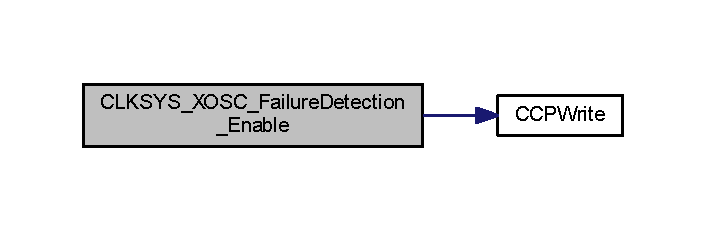
\includegraphics[width=339pt]{clksys__driver_8h_abfb0da2d81736412af825d46e7e0cedb_cgraph}
\end{center}
\end{figure}

\hypertarget{clock_8c}{}\section{clock.\+c File Reference}
\label{clock_8c}\index{clock.\+c@{clock.\+c}}


This file contains the Function to init, calibrate and change the clock.  


{\ttfamily \#include \char`\"{}clock.\+h\char`\"{}}\newline
Include dependency graph for clock.\+c\+:\nopagebreak
\begin{figure}[H]
\begin{center}
\leavevmode
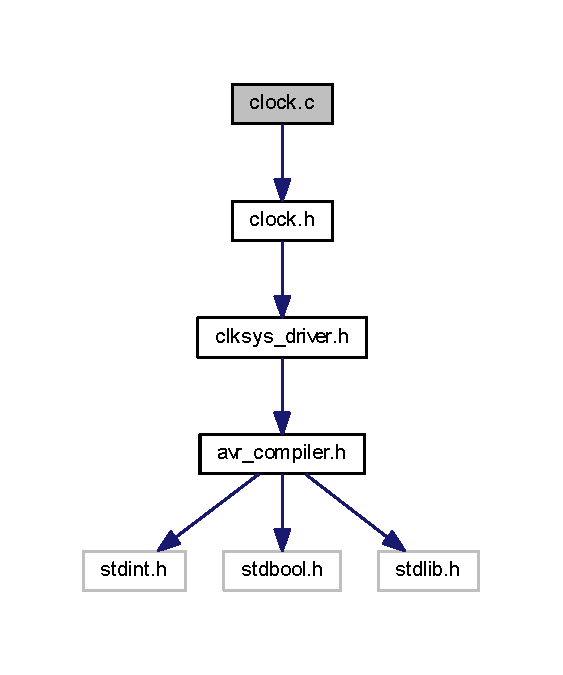
\includegraphics[width=270pt]{clock_8c__incl}
\end{center}
\end{figure}
\subsection*{Macros}
\begin{DoxyCompactItemize}
\item 
\#define \hyperlink{clock_8c_a43bafb28b29491ec7f871319b5a3b2f8}{F\+\_\+\+C\+PU}~32000000\+UL
\end{DoxyCompactItemize}
\subsection*{Functions}
\begin{DoxyCompactItemize}
\item 
void \hyperlink{clock_8c_a23a363c676847b1b84e6149472897fa2}{set\+\_\+clock\+\_\+32\+M\+Hz} (void)
\begin{DoxyCompactList}\small\item\em This function inits, calibrates and changes the clock. \end{DoxyCompactList}\end{DoxyCompactItemize}


\subsection{Detailed Description}
This file contains the Function to init, calibrate and change the clock. 

\begin{DoxyAuthor}{Author}
Jan Baudis 
\end{DoxyAuthor}
\begin{DoxyDate}{Date}
11.\+09.\+2016 14\+:24\+:30 
\end{DoxyDate}


\subsection{Macro Definition Documentation}
\hypertarget{clock_8c_a43bafb28b29491ec7f871319b5a3b2f8}{}\label{clock_8c_a43bafb28b29491ec7f871319b5a3b2f8} 
\index{clock.\+c@{clock.\+c}!F\+\_\+\+C\+PU@{F\+\_\+\+C\+PU}}
\index{F\+\_\+\+C\+PU@{F\+\_\+\+C\+PU}!clock.\+c@{clock.\+c}}
\subsubsection{\texorpdfstring{F\+\_\+\+C\+PU}{F\_CPU}}
{\footnotesize\ttfamily \#define F\+\_\+\+C\+PU~32000000\+UL}



\subsection{Function Documentation}
\hypertarget{clock_8c_a23a363c676847b1b84e6149472897fa2}{}\label{clock_8c_a23a363c676847b1b84e6149472897fa2} 
\index{clock.\+c@{clock.\+c}!set\+\_\+clock\+\_\+32\+M\+Hz@{set\+\_\+clock\+\_\+32\+M\+Hz}}
\index{set\+\_\+clock\+\_\+32\+M\+Hz@{set\+\_\+clock\+\_\+32\+M\+Hz}!clock.\+c@{clock.\+c}}
\subsubsection{\texorpdfstring{set\+\_\+clock\+\_\+32\+M\+Hz()}{set\_clock\_32MHz()}}
{\footnotesize\ttfamily void set\+\_\+clock\+\_\+32\+M\+Hz (\begin{DoxyParamCaption}\item[{void}]{ }\end{DoxyParamCaption})}



This function inits, calibrates and changes the clock. 

It enables the 32k\+Hz ref Clock for the Autocalibration and also executes the calibration. Afterwards it enables and changes to the 32\+M\+Hz internal Clock and also disables the 2\+M\+Hz \& 32k\+Hz clocks. Eventually it Locks the current Clock config. 

Definition at line 16 of file clock.\+c.



References C\+L\+K\+S\+Y\+S\+\_\+\+Auto\+Calibration\+\_\+\+Enable(), C\+L\+K\+S\+Y\+S\+\_\+\+Configuration\+\_\+\+Lock(), C\+L\+K\+S\+Y\+S\+\_\+\+Disable(), C\+L\+K\+S\+Y\+S\+\_\+\+Enable, C\+L\+K\+S\+Y\+S\+\_\+\+Is\+Ready, and C\+L\+K\+S\+Y\+S\+\_\+\+Main\+\_\+\+Clock\+Source\+\_\+\+Select().



Referenced by main().

Here is the call graph for this function\+:\nopagebreak
\begin{figure}[H]
\begin{center}
\leavevmode
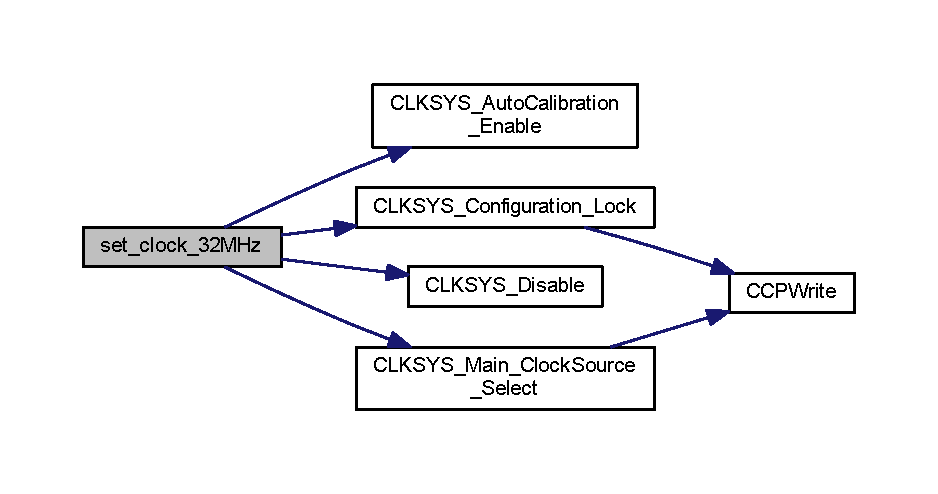
\includegraphics[width=350pt]{clock_8c_a23a363c676847b1b84e6149472897fa2_cgraph}
\end{center}
\end{figure}
Here is the caller graph for this function\+:\nopagebreak
\begin{figure}[H]
\begin{center}
\leavevmode
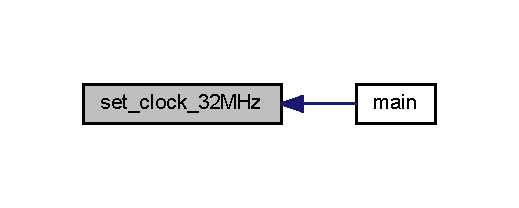
\includegraphics[width=249pt]{clock_8c_a23a363c676847b1b84e6149472897fa2_icgraph}
\end{center}
\end{figure}

\hypertarget{clock_8h}{}\section{clock.\+h File Reference}
\label{clock_8h}\index{clock.\+h@{clock.\+h}}


This file is the Headerfile for the clock-\/\+File. It contains the prototypes of the functions and the usual macros.  


{\ttfamily \#include \char`\"{}clksys\+\_\+driver.\+h\char`\"{}}\newline
Include dependency graph for clock.\+h\+:\nopagebreak
\begin{figure}[H]
\begin{center}
\leavevmode
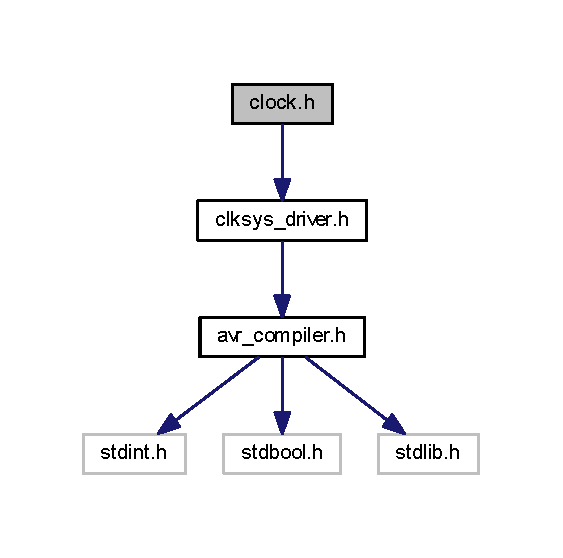
\includegraphics[width=270pt]{clock_8h__incl}
\end{center}
\end{figure}
This graph shows which files directly or indirectly include this file\+:\nopagebreak
\begin{figure}[H]
\begin{center}
\leavevmode
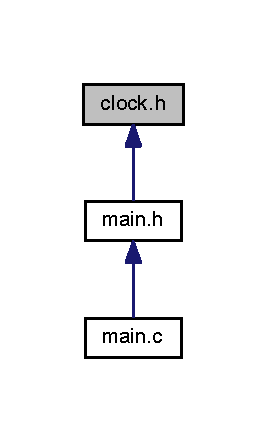
\includegraphics[width=192pt]{clock_8h__dep__incl}
\end{center}
\end{figure}
\subsection*{Functions}
\begin{DoxyCompactItemize}
\item 
void \hyperlink{clock_8h_a23a363c676847b1b84e6149472897fa2}{set\+\_\+clock\+\_\+32\+M\+Hz} (void)
\begin{DoxyCompactList}\small\item\em This function inits, calibrates and changes the clock. \end{DoxyCompactList}\end{DoxyCompactItemize}


\subsection{Detailed Description}
This file is the Headerfile for the clock-\/\+File. It contains the prototypes of the functions and the usual macros. 

\begin{DoxyAuthor}{Author}
Jan Baudis 
\end{DoxyAuthor}
\begin{DoxyDate}{Date}
11.\+09.\+2016 14\+:24\+:45 
\end{DoxyDate}


\subsection{Function Documentation}
\hypertarget{clock_8h_a23a363c676847b1b84e6149472897fa2}{}\label{clock_8h_a23a363c676847b1b84e6149472897fa2} 
\index{clock.\+h@{clock.\+h}!set\+\_\+clock\+\_\+32\+M\+Hz@{set\+\_\+clock\+\_\+32\+M\+Hz}}
\index{set\+\_\+clock\+\_\+32\+M\+Hz@{set\+\_\+clock\+\_\+32\+M\+Hz}!clock.\+h@{clock.\+h}}
\subsubsection{\texorpdfstring{set\+\_\+clock\+\_\+32\+M\+Hz()}{set\_clock\_32MHz()}}
{\footnotesize\ttfamily void set\+\_\+clock\+\_\+32\+M\+Hz (\begin{DoxyParamCaption}\item[{void}]{ }\end{DoxyParamCaption})}



This function inits, calibrates and changes the clock. 

It enables the 32k\+Hz ref Clock for the Autocalibration and also executes the calibration. Afterwards it enables and changes to the 32\+M\+Hz internal Clock and also disables the 2\+M\+Hz \& 32k\+Hz clocks. Eventually it Locks the current Clock config. 

Definition at line 16 of file clock.\+c.



References C\+L\+K\+S\+Y\+S\+\_\+\+Auto\+Calibration\+\_\+\+Enable(), C\+L\+K\+S\+Y\+S\+\_\+\+Configuration\+\_\+\+Lock(), C\+L\+K\+S\+Y\+S\+\_\+\+Disable(), C\+L\+K\+S\+Y\+S\+\_\+\+Enable, C\+L\+K\+S\+Y\+S\+\_\+\+Is\+Ready, and C\+L\+K\+S\+Y\+S\+\_\+\+Main\+\_\+\+Clock\+Source\+\_\+\+Select().



Referenced by main().

Here is the call graph for this function\+:\nopagebreak
\begin{figure}[H]
\begin{center}
\leavevmode
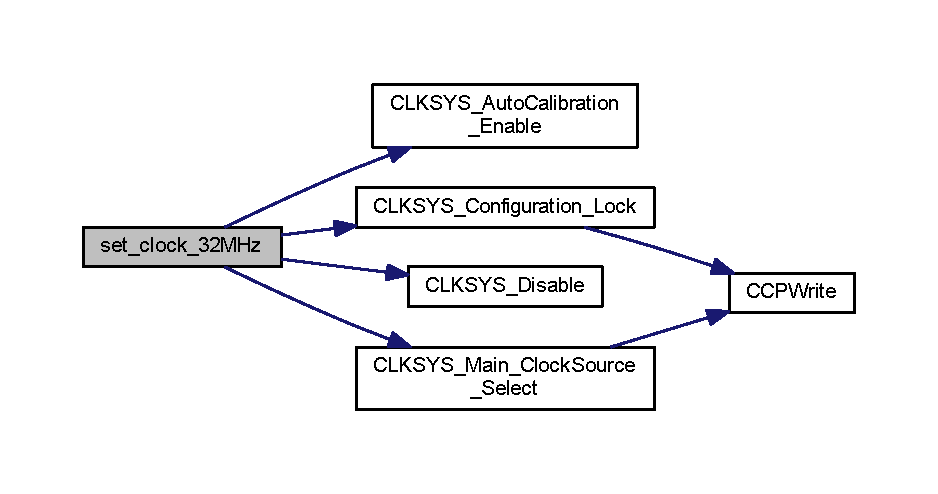
\includegraphics[width=350pt]{clock_8h_a23a363c676847b1b84e6149472897fa2_cgraph}
\end{center}
\end{figure}
Here is the caller graph for this function\+:\nopagebreak
\begin{figure}[H]
\begin{center}
\leavevmode
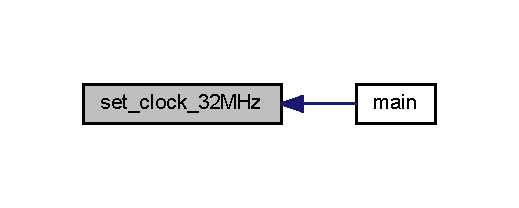
\includegraphics[width=249pt]{clock_8h_a23a363c676847b1b84e6149472897fa2_icgraph}
\end{center}
\end{figure}

\hypertarget{main_8c}{}\section{main.\+c File Reference}
\label{main_8c}\index{main.\+c@{main.\+c}}


This file is the main-\/\+File. It calls all the fancy Functions and so on.  


{\ttfamily \#include \char`\"{}main.\+h\char`\"{}}\newline
{\ttfamily \#include \char`\"{}U\+A\+R\+T.\+h\char`\"{}}\newline
Include dependency graph for main.\+c\+:
% FIG 0
\subsection*{Functions}
\begin{DoxyCompactItemize}
\item 
uint8\+\_\+t \hyperlink{main_8c_a69539018526f1fb80d3cf1c91bb08911}{U\+S\+A\+R\+T\+\_\+test} (\hyperlink{usart__driver_8h_a884c38d38327b0d4263c03cf0d84031e}{U\+S\+A\+R\+T\+\_\+data\+\_\+t} $\ast$usart\+\_\+data)
\item 
int \hyperlink{main_8c_a840291bc02cba5474a4cb46a9b9566fe}{main} (void)
\begin{DoxyCompactList}\small\item\em This is the main-\/\+Function. \end{DoxyCompactList}\end{DoxyCompactItemize}
\subsection*{Variables}
\begin{DoxyCompactItemize}
\item 
int volatile \hyperlink{main_8c_a37fd7702e47867237a1617ae4b4fab85}{ret\+\_\+pressed}
\end{DoxyCompactItemize}


\subsection{Detailed Description}
This file is the main-\/\+File. It calls all the fancy Functions and so on. 

\begin{DoxyAuthor}{Author}
Jan Baudis 
\end{DoxyAuthor}
\begin{DoxyDate}{Date}
08.\+09.\+2016 01\+:50\+:07 
\end{DoxyDate}


\subsection{Function Documentation}
\hypertarget{main_8c_a840291bc02cba5474a4cb46a9b9566fe}{}\label{main_8c_a840291bc02cba5474a4cb46a9b9566fe} 
\index{main.\+c@{main.\+c}!main@{main}}
\index{main@{main}!main.\+c@{main.\+c}}
\subsubsection{\texorpdfstring{main()}{main()}}
{\footnotesize\ttfamily int main (\begin{DoxyParamCaption}\item[{void}]{ }\end{DoxyParamCaption})}



This is the main-\/\+Function. 

It calls all the fancy Functions. It does things. Enter the \char`\"{}\+Shell\char`\"{}! 

Definition at line 29 of file main.\+c.



References enter\+\_\+shell(), receive\+\_\+string\+\_\+from\+\_\+usart(), ret\+\_\+pressed, send\+\_\+string\+\_\+pgm\+\_\+to\+\_\+usart(), send\+\_\+string\+\_\+to\+\_\+usart(), set\+\_\+clock\+\_\+32\+M\+Hz(), U\+S\+A\+R\+T\+\_\+\+D\+A\+T\+A\+\_\+\+PC, usart\+\_\+init\+\_\+pc(), and usart\+\_\+init\+\_\+tpuart().

Here is the call graph for this function\+:
% FIG 1
\hypertarget{main_8c_a69539018526f1fb80d3cf1c91bb08911}{}\label{main_8c_a69539018526f1fb80d3cf1c91bb08911} 
\index{main.\+c@{main.\+c}!U\+S\+A\+R\+T\+\_\+test@{U\+S\+A\+R\+T\+\_\+test}}
\index{U\+S\+A\+R\+T\+\_\+test@{U\+S\+A\+R\+T\+\_\+test}!main.\+c@{main.\+c}}
\subsubsection{\texorpdfstring{U\+S\+A\+R\+T\+\_\+test()}{USART\_test()}}
{\footnotesize\ttfamily uint8\+\_\+t U\+S\+A\+R\+T\+\_\+test (\begin{DoxyParamCaption}\item[{\hyperlink{usart__driver_8h_a884c38d38327b0d4263c03cf0d84031e}{U\+S\+A\+R\+T\+\_\+data\+\_\+t} $\ast$}]{usart\+\_\+data }\end{DoxyParamCaption})}



Definition at line 12 of file main.\+c.



References Usart\+\_\+and\+\_\+buffer\+::buffer, U\+S\+A\+R\+T\+\_\+\+Buffer\+::\+RX, and U\+S\+A\+R\+T\+\_\+\+Buffer\+::\+R\+X\+\_\+\+Tail.



\subsection{Variable Documentation}
\hypertarget{main_8c_a37fd7702e47867237a1617ae4b4fab85}{}\label{main_8c_a37fd7702e47867237a1617ae4b4fab85} 
\index{main.\+c@{main.\+c}!ret\+\_\+pressed@{ret\+\_\+pressed}}
\index{ret\+\_\+pressed@{ret\+\_\+pressed}!main.\+c@{main.\+c}}
\subsubsection{\texorpdfstring{ret\+\_\+pressed}{ret\_pressed}}
{\footnotesize\ttfamily int volatile ret\+\_\+pressed}



Definition at line 11 of file U\+A\+R\+T.\+c.



Referenced by main().


\hypertarget{main_8h}{}\section{main.\+h File Reference}
\label{main_8h}\index{main.\+h@{main.\+h}}


This file is the Headerfile for the main-\/\+File. It contains general things like the F\+\_\+\+C\+PU Macro etc.  


{\ttfamily \#include $<$avr/io.\+h$>$}\newline
{\ttfamily \#include \char`\"{}clksys\+\_\+driver.\+h\char`\"{}}\newline
{\ttfamily \#include \char`\"{}clock.\+h\char`\"{}}\newline
Include dependency graph for main.\+h\+:\nopagebreak
\begin{figure}[H]
\begin{center}
\leavevmode
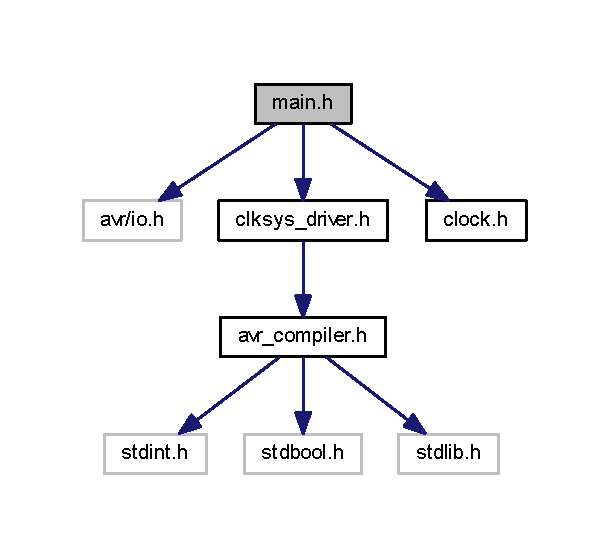
\includegraphics[width=293pt]{main_8h__incl}
\end{center}
\end{figure}
This graph shows which files directly or indirectly include this file\+:\nopagebreak
\begin{figure}[H]
\begin{center}
\leavevmode
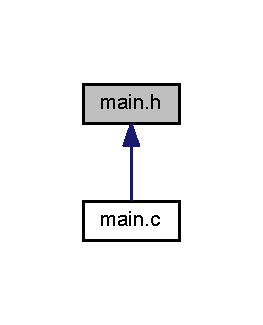
\includegraphics[width=126pt]{main_8h__dep__incl}
\end{center}
\end{figure}


\subsection{Detailed Description}
This file is the Headerfile for the main-\/\+File. It contains general things like the F\+\_\+\+C\+PU Macro etc. 

\begin{DoxyAuthor}{Author}
Jan Baudis 
\end{DoxyAuthor}

\hypertarget{shell_8c}{}\section{shell.\+c File Reference}
\label{shell_8c}\index{shell.\+c@{shell.\+c}}


Implements a basic \char`\"{}shell\char`\"{} to communicate with the T\+P\+U\+A\+R\+T/\+K\+NX and Debug things. Data sheet K\+NX E\+IB T\+P-\/\+U\+A\+RT 2+ page 22 and following.  


{\ttfamily \#include \char`\"{}shell.\+h\char`\"{}}\newline
Include dependency graph for shell.\+c\+:\nopagebreak
\begin{figure}[H]
\begin{center}
\leavevmode
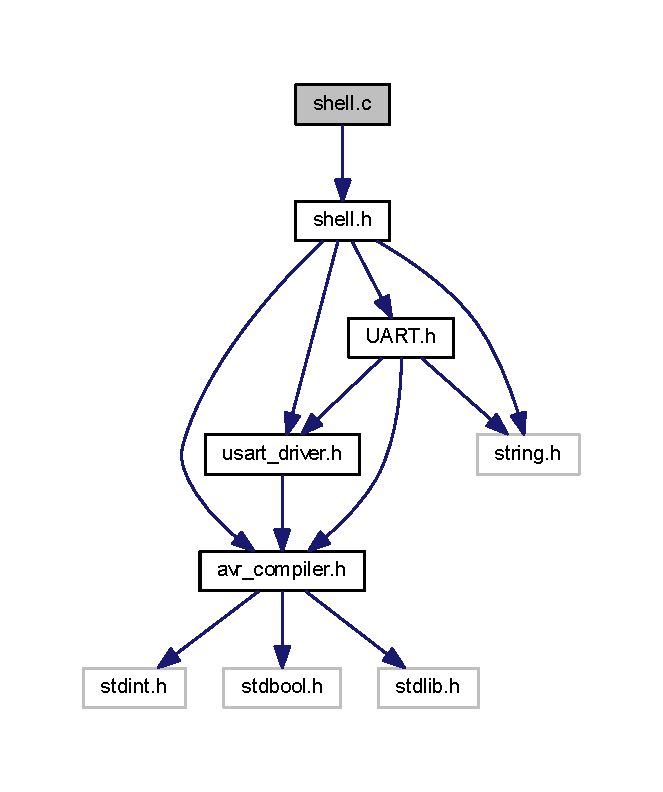
\includegraphics[width=318pt]{shell_8c__incl}
\end{center}
\end{figure}
\subsection*{Functions}
\begin{DoxyCompactItemize}
\item 
void \hyperlink{shell_8c_a3197713442e02b97406567e4a11e193f}{enter\+\_\+shell} (\hyperlink{usart__driver_8h_a884c38d38327b0d4263c03cf0d84031e}{U\+S\+A\+R\+T\+\_\+data\+\_\+t} $\ast$U\+S\+A\+R\+T\+\_\+data)
\begin{DoxyCompactList}\small\item\em Enter the \char`\"{}\+Shell\char`\"{}. \end{DoxyCompactList}\item 
void \hyperlink{shell_8c_ab8aa91cc93dc57699d69cf98e7244d64}{reset\+\_\+request} (void)
\begin{DoxyCompactList}\small\item\em Shell-\/\+Function for the U\+\_\+reset.\+request-\/\+Service. \end{DoxyCompactList}\item 
void \hyperlink{shell_8c_a7e7bbbb940671ab75e317fb9e82e956d}{state\+\_\+request} (void)
\begin{DoxyCompactList}\small\item\em Shell-\/\+Function for the U\+\_\+state.\+request-\/\+Service. \end{DoxyCompactList}\item 
void \hyperlink{shell_8c_ad95c9c45c97cc744ca49a98494bf9465}{act\+\_\+busmon} (void)
\begin{DoxyCompactList}\small\item\em Shell-\/\+Function for the U\+\_\+\+Activate\+Busmon-\/\+Service. \end{DoxyCompactList}\item 
void \hyperlink{shell_8c_aef27926c3ebc8dc98a95df932af53a06}{prod\+\_\+request} (void)
\begin{DoxyCompactList}\small\item\em Shell-\/\+Function for the U\+\_\+\+Product\+I\+D.\+request-\/\+Service. \end{DoxyCompactList}\item 
void \hyperlink{shell_8c_a5c364cd022ec191bccd57afa8aae1e89}{act\+\_\+busymode} (void)
\begin{DoxyCompactList}\small\item\em Shell-\/\+Function for the U\+\_\+\+Activate\+Busy\+Mode. \end{DoxyCompactList}\item 
void \hyperlink{shell_8c_acd8340ade32d7f467cf3b625bd06ba31}{shell\+\_\+help} (void)
\end{DoxyCompactItemize}
\subsection*{Variables}
\begin{DoxyCompactItemize}
\item 
int volatile \hyperlink{shell_8c_a37fd7702e47867237a1617ae4b4fab85}{ret\+\_\+pressed}
\item 
char \hyperlink{shell_8c_a68426a3f72e0fa2063f5140143c60965}{command} \mbox{[}33\mbox{]}
\end{DoxyCompactItemize}


\subsection{Detailed Description}
Implements a basic \char`\"{}shell\char`\"{} to communicate with the T\+P\+U\+A\+R\+T/\+K\+NX and Debug things. Data sheet K\+NX E\+IB T\+P-\/\+U\+A\+RT 2+ page 22 and following. 

\begin{DoxyAuthor}{Author}
Jan Baudis 
\end{DoxyAuthor}
\begin{DoxyDate}{Date}
03.\+12.\+2016 01\+:01\+:54 
\end{DoxyDate}
\begin{DoxyNote}{Note}
Buffer Size in the \hyperlink{usart__driver_8h}{usart\+\_\+driver.\+h} has to be changed if the commands are too big -\/ it only evaluates the received string when enter is pressed. 
\end{DoxyNote}
\begin{DoxyRefDesc}{Todo}
\item[\hyperlink{todo__todo000001}{Todo}]Maybe disable RX for the PC while working on a command! \end{DoxyRefDesc}


\subsection{Function Documentation}
\hypertarget{shell_8c_ad95c9c45c97cc744ca49a98494bf9465}{}\label{shell_8c_ad95c9c45c97cc744ca49a98494bf9465} 
\index{shell.\+c@{shell.\+c}!act\+\_\+busmon@{act\+\_\+busmon}}
\index{act\+\_\+busmon@{act\+\_\+busmon}!shell.\+c@{shell.\+c}}
\subsubsection{\texorpdfstring{act\+\_\+busmon()}{act\_busmon()}}
{\footnotesize\ttfamily void act\+\_\+busmon (\begin{DoxyParamCaption}\item[{void}]{ }\end{DoxyParamCaption})}



Shell-\/\+Function for the U\+\_\+\+Activate\+Busmon-\/\+Service. 

Sends the U\+\_\+\+Activate\+Busmon to the T\+P\+U\+A\+RT and prints the Output as bits to the PC. Listens till it receives any Key from the PC. Then it Resets the Chip since its the Only way to quit the Busmon-\/\+Mode of the T\+P\+U\+A\+RT.

\begin{DoxyRefDesc}{Todo}
\item[\hyperlink{todo__todo000002}{Todo}]Implement an end of Packet detection to print out some useful Information for the Bits.\end{DoxyRefDesc}


Definition at line 175 of file shell.\+c.



References command, flush\+\_\+\+U\+S\+A\+R\+T\+\_\+\+R\+X\+Buffer(), receive\+\_\+string\+\_\+from\+\_\+usart(), reset\+\_\+request(), send\+\_\+string\+\_\+pgm\+\_\+to\+\_\+usart(), send\+\_\+string\+\_\+to\+\_\+usart(), U\+S\+A\+R\+T\+\_\+\+D\+A\+T\+A\+\_\+\+PC, U\+S\+A\+R\+T\+\_\+\+D\+A\+T\+A\+\_\+\+TP, U\+S\+A\+R\+T\+\_\+\+R\+X\+\_\+\+B\+U\+F\+F\+E\+R\+\_\+\+S\+I\+ZE, U\+S\+A\+R\+T\+\_\+\+R\+X\+Buffer\+Data\+\_\+\+Available(), and U\+S\+A\+R\+T\+\_\+\+T\+X\+Buffer\+\_\+\+Put\+Byte().



Referenced by enter\+\_\+shell().

Here is the call graph for this function\+:
\nopagebreak
\begin{figure}[H]
\begin{center}
\leavevmode
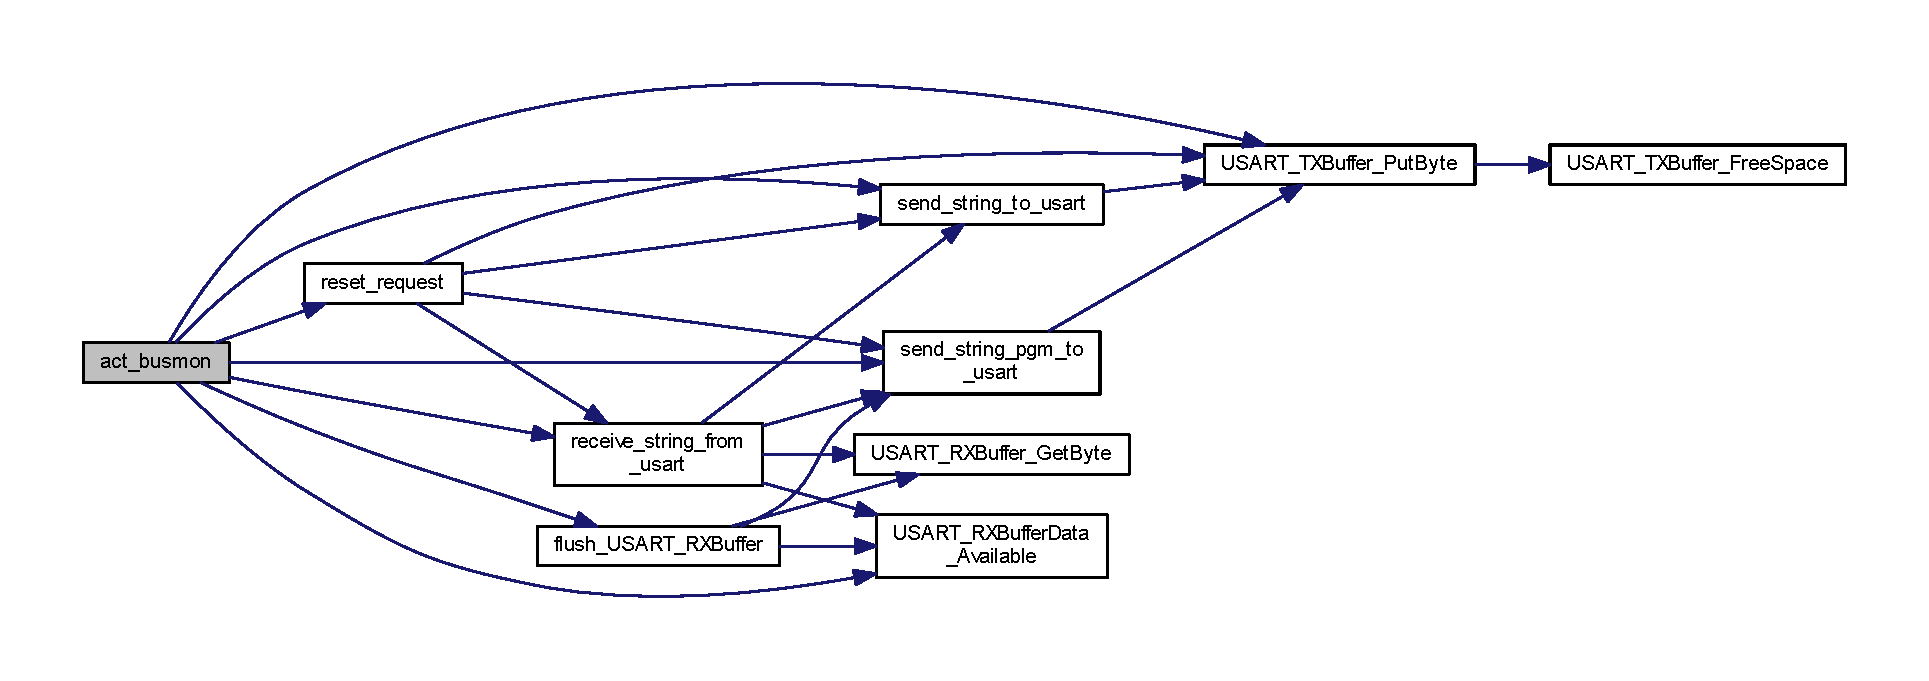
\includegraphics[width=350pt]{shell_8c_ad95c9c45c97cc744ca49a98494bf9465_cgraph}
\end{center}
\end{figure}
Here is the caller graph for this function\+:
\nopagebreak
\begin{figure}[H]
\begin{center}
\leavevmode
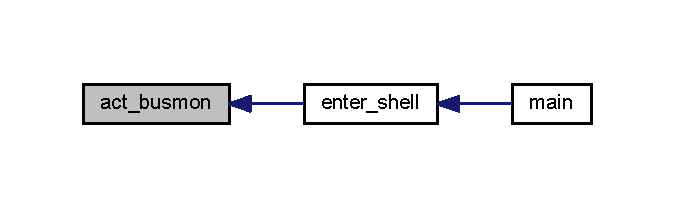
\includegraphics[width=324pt]{shell_8c_ad95c9c45c97cc744ca49a98494bf9465_icgraph}
\end{center}
\end{figure}
\hypertarget{shell_8c_a5c364cd022ec191bccd57afa8aae1e89}{}\label{shell_8c_a5c364cd022ec191bccd57afa8aae1e89} 
\index{shell.\+c@{shell.\+c}!act\+\_\+busymode@{act\+\_\+busymode}}
\index{act\+\_\+busymode@{act\+\_\+busymode}!shell.\+c@{shell.\+c}}
\subsubsection{\texorpdfstring{act\+\_\+busymode()}{act\_busymode()}}
{\footnotesize\ttfamily void act\+\_\+busymode (\begin{DoxyParamCaption}\item[{void}]{ }\end{DoxyParamCaption})}



Shell-\/\+Function for the U\+\_\+\+Activate\+Busy\+Mode. 

Sends the U\+\_\+\+Activate\+Busy\+Mode to the T\+P\+U\+A\+RT and prints the Output as bits to the PC. T\+P-\/\+U\+A\+RT responses on every Packet which is addressed to him with B\+U\+SY within 700ms (+-\/10ms). All Packets are send to the Host and if the Host confirms one with U\+\_\+\+Ackinfo it will leave Busy\+Mode as well when reseted.

\begin{DoxyRefDesc}{Todo}
\item[\hyperlink{todo__todo000003}{Todo}]May add something; Dunno like a Listen Mode for 700ms; \end{DoxyRefDesc}


Definition at line 268 of file shell.\+c.



References command, prod\+\_\+request(), receive\+\_\+string\+\_\+from\+\_\+usart(), send\+\_\+string\+\_\+pgm\+\_\+to\+\_\+usart(), send\+\_\+string\+\_\+to\+\_\+usart(), U\+S\+A\+R\+T\+\_\+\+D\+A\+T\+A\+\_\+\+PC, U\+S\+A\+R\+T\+\_\+\+D\+A\+T\+A\+\_\+\+TP, U\+S\+A\+R\+T\+\_\+\+R\+X\+\_\+\+B\+U\+F\+F\+E\+R\+\_\+\+S\+I\+ZE, and U\+S\+A\+R\+T\+\_\+\+T\+X\+Buffer\+\_\+\+Put\+Byte().



Referenced by enter\+\_\+shell().

Here is the call graph for this function\+:
\nopagebreak
\begin{figure}[H]
\begin{center}
\leavevmode
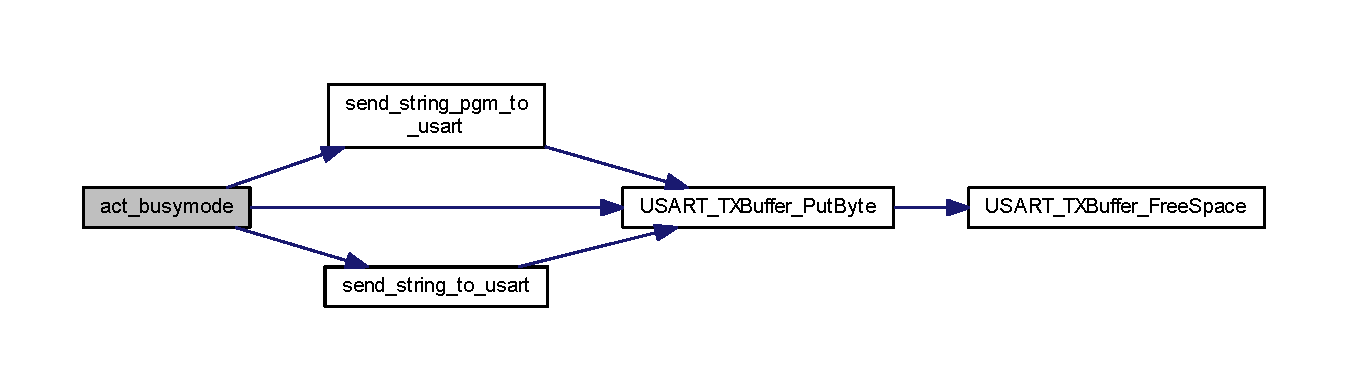
\includegraphics[width=350pt]{shell_8c_a5c364cd022ec191bccd57afa8aae1e89_cgraph}
\end{center}
\end{figure}
Here is the caller graph for this function\+:
\nopagebreak
\begin{figure}[H]
\begin{center}
\leavevmode
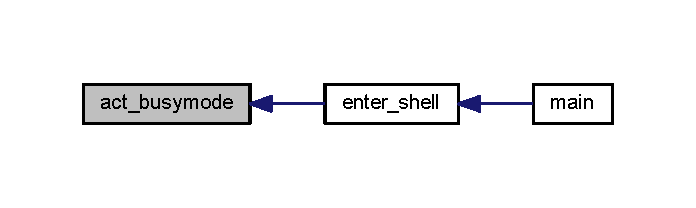
\includegraphics[width=334pt]{shell_8c_a5c364cd022ec191bccd57afa8aae1e89_icgraph}
\end{center}
\end{figure}
\hypertarget{shell_8c_a3197713442e02b97406567e4a11e193f}{}\label{shell_8c_a3197713442e02b97406567e4a11e193f} 
\index{shell.\+c@{shell.\+c}!enter\+\_\+shell@{enter\+\_\+shell}}
\index{enter\+\_\+shell@{enter\+\_\+shell}!shell.\+c@{shell.\+c}}
\subsubsection{\texorpdfstring{enter\+\_\+shell()}{enter\_shell()}}
{\footnotesize\ttfamily void enter\+\_\+shell (\begin{DoxyParamCaption}\item[{\hyperlink{usart__driver_8h_a884c38d38327b0d4263c03cf0d84031e}{U\+S\+A\+R\+T\+\_\+data\+\_\+t} $\ast$}]{U\+S\+A\+R\+T\+\_\+data }\end{DoxyParamCaption})}



Enter the \char`\"{}\+Shell\char`\"{}. 

In the \char`\"{}\+Shell\char`\"{} we can e.\+g. use the Services of the T\+P\+U\+A\+RT


\begin{DoxyParams}{Parameters}
{\em U\+S\+A\+R\+T\+\_\+data} & The U\+S\+A\+R\+T\+\_\+data\+\_\+t struct instance. \\
\hline
\end{DoxyParams}


Definition at line 22 of file shell.\+c.



References act\+\_\+busmon(), act\+\_\+busymode(), command, prod\+\_\+request(), receive\+\_\+string\+\_\+from\+\_\+usart(), reset\+\_\+request(), ret\+\_\+pressed, send\+\_\+string\+\_\+pgm\+\_\+to\+\_\+usart(), send\+\_\+string\+\_\+to\+\_\+usart(), shell\+\_\+help(), state\+\_\+request(), and U\+S\+A\+R\+T\+\_\+\+D\+A\+T\+A\+\_\+\+PC.



Referenced by main().

Here is the call graph for this function\+:
\nopagebreak
\begin{figure}[H]
\begin{center}
\leavevmode
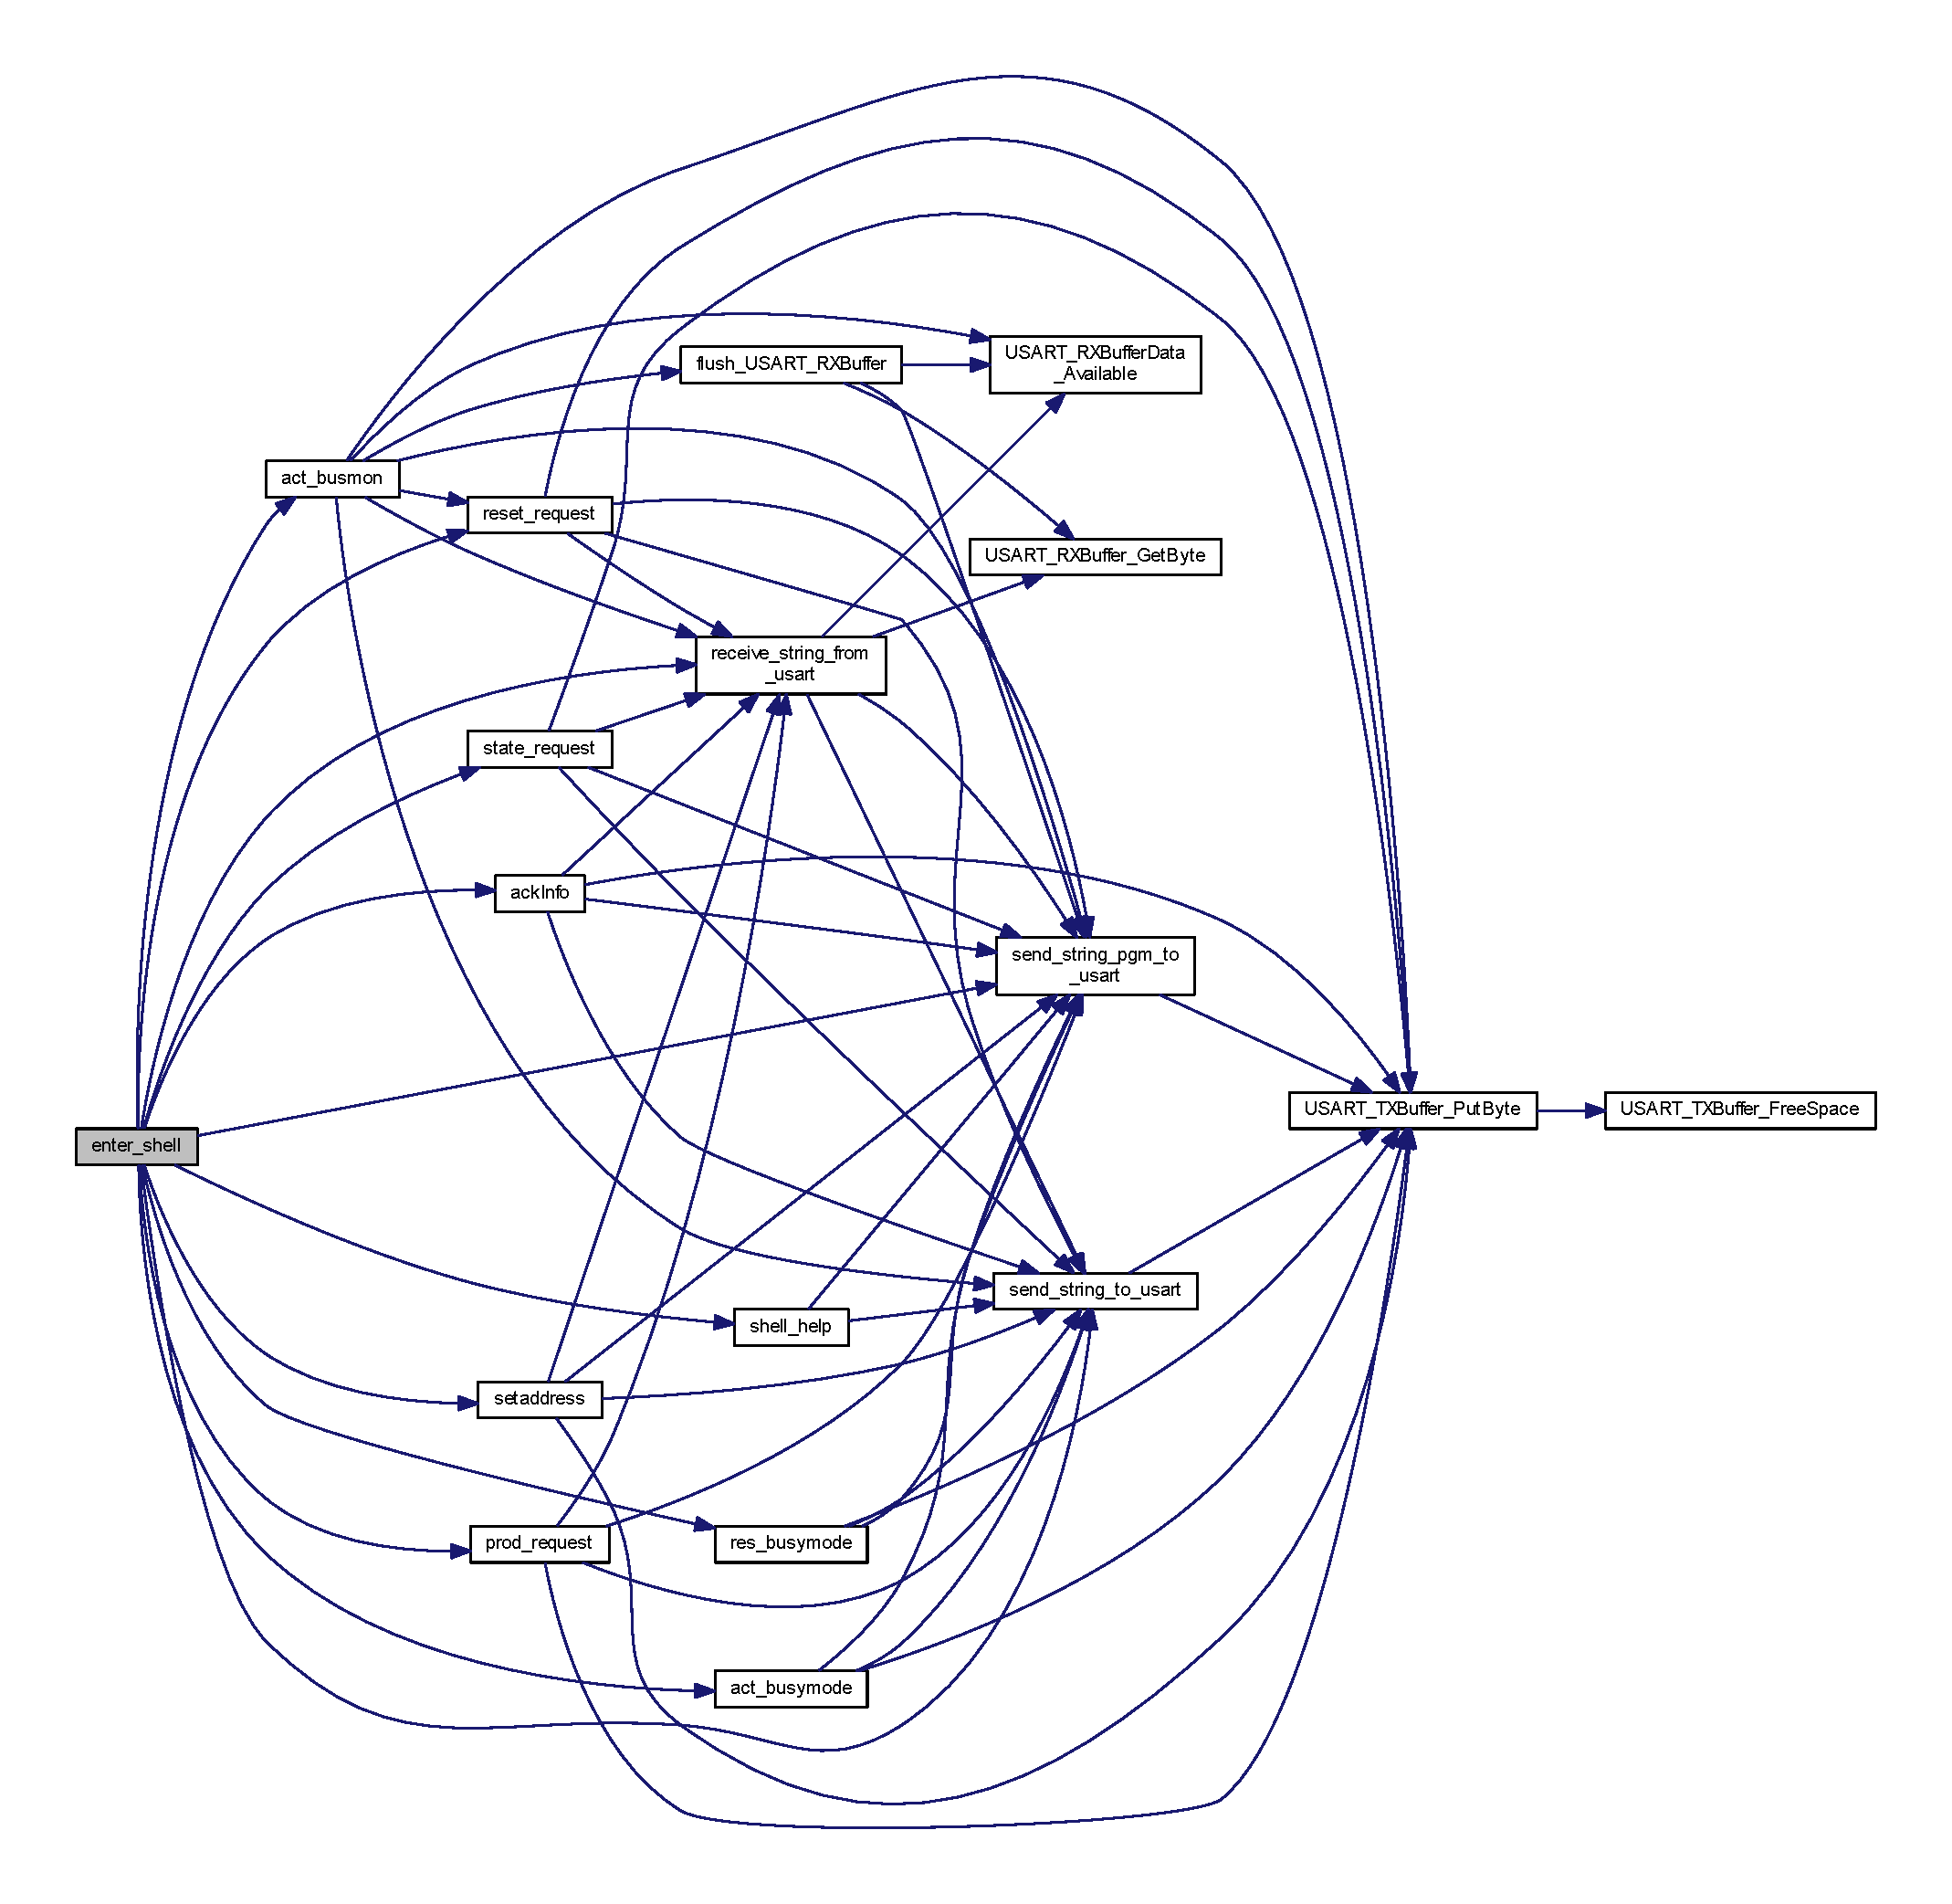
\includegraphics[width=350pt]{shell_8c_a3197713442e02b97406567e4a11e193f_cgraph}
\end{center}
\end{figure}
Here is the caller graph for this function\+:
\nopagebreak
\begin{figure}[H]
\begin{center}
\leavevmode
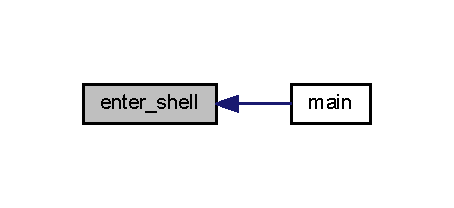
\includegraphics[width=218pt]{shell_8c_a3197713442e02b97406567e4a11e193f_icgraph}
\end{center}
\end{figure}
\hypertarget{shell_8c_aef27926c3ebc8dc98a95df932af53a06}{}\label{shell_8c_aef27926c3ebc8dc98a95df932af53a06} 
\index{shell.\+c@{shell.\+c}!prod\+\_\+request@{prod\+\_\+request}}
\index{prod\+\_\+request@{prod\+\_\+request}!shell.\+c@{shell.\+c}}
\subsubsection{\texorpdfstring{prod\+\_\+request()}{prod\_request()}}
{\footnotesize\ttfamily void prod\+\_\+request (\begin{DoxyParamCaption}\item[{void}]{ }\end{DoxyParamCaption})}



Shell-\/\+Function for the U\+\_\+\+Product\+I\+D.\+request-\/\+Service. 

Sends the U\+\_\+\+Product\+I\+D.\+request to the T\+P\+U\+A\+RT and prints the Output as bits to the PC 

Definition at line 224 of file shell.\+c.



References command, receive\+\_\+string\+\_\+from\+\_\+usart(), send\+\_\+string\+\_\+pgm\+\_\+to\+\_\+usart(), send\+\_\+string\+\_\+to\+\_\+usart(), U\+S\+A\+R\+T\+\_\+\+D\+A\+T\+A\+\_\+\+PC, U\+S\+A\+R\+T\+\_\+\+D\+A\+T\+A\+\_\+\+TP, U\+S\+A\+R\+T\+\_\+\+R\+X\+\_\+\+B\+U\+F\+F\+E\+R\+\_\+\+S\+I\+ZE, and U\+S\+A\+R\+T\+\_\+\+T\+X\+Buffer\+\_\+\+Put\+Byte().



Referenced by act\+\_\+busymode(), and enter\+\_\+shell().

Here is the call graph for this function\+:
\nopagebreak
\begin{figure}[H]
\begin{center}
\leavevmode
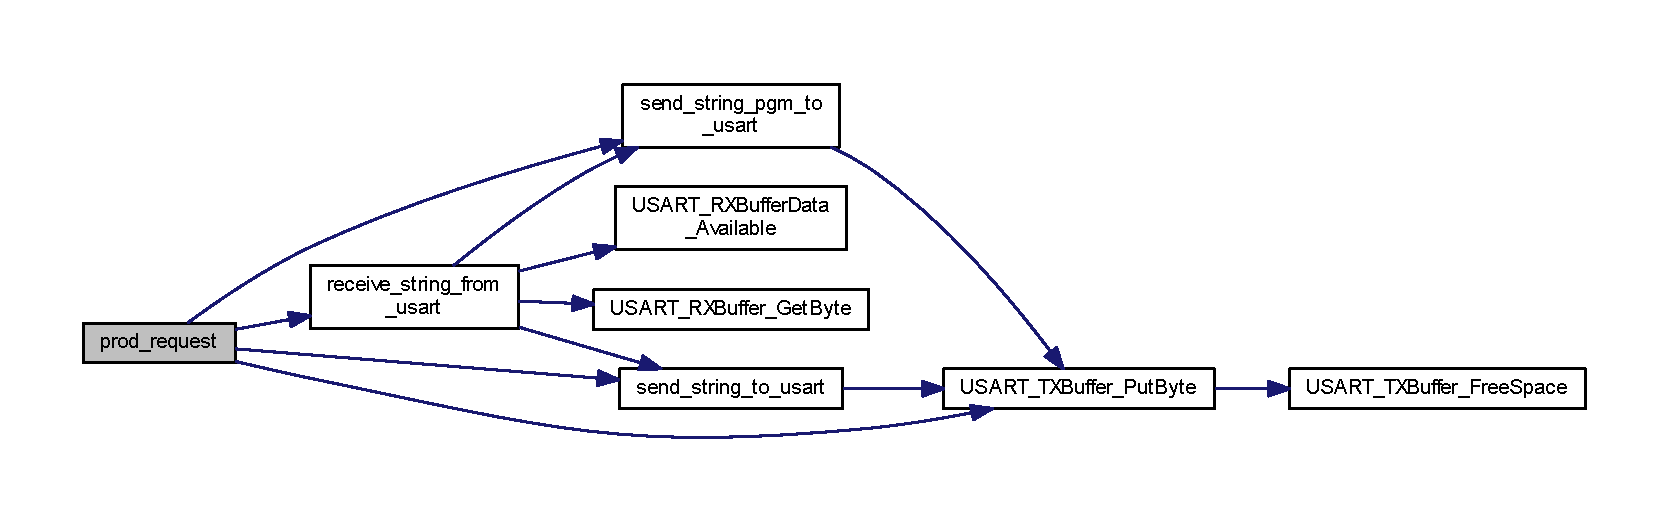
\includegraphics[width=350pt]{shell_8c_aef27926c3ebc8dc98a95df932af53a06_cgraph}
\end{center}
\end{figure}
Here is the caller graph for this function\+:
\nopagebreak
\begin{figure}[H]
\begin{center}
\leavevmode
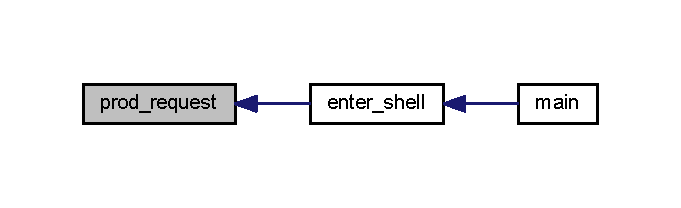
\includegraphics[width=350pt]{shell_8c_aef27926c3ebc8dc98a95df932af53a06_icgraph}
\end{center}
\end{figure}
\hypertarget{shell_8c_ab8aa91cc93dc57699d69cf98e7244d64}{}\label{shell_8c_ab8aa91cc93dc57699d69cf98e7244d64} 
\index{shell.\+c@{shell.\+c}!reset\+\_\+request@{reset\+\_\+request}}
\index{reset\+\_\+request@{reset\+\_\+request}!shell.\+c@{shell.\+c}}
\subsubsection{\texorpdfstring{reset\+\_\+request()}{reset\_request()}}
{\footnotesize\ttfamily void reset\+\_\+request (\begin{DoxyParamCaption}\item[{void}]{ }\end{DoxyParamCaption})}



Shell-\/\+Function for the U\+\_\+reset.\+request-\/\+Service. 

Sends the U\+\_\+reset.\+request to the T\+P\+U\+A\+RT and prints the Output as bits to the PC 

Definition at line 89 of file shell.\+c.



References command, receive\+\_\+string\+\_\+from\+\_\+usart(), send\+\_\+string\+\_\+pgm\+\_\+to\+\_\+usart(), send\+\_\+string\+\_\+to\+\_\+usart(), U\+S\+A\+R\+T\+\_\+\+D\+A\+T\+A\+\_\+\+PC, U\+S\+A\+R\+T\+\_\+\+D\+A\+T\+A\+\_\+\+TP, U\+S\+A\+R\+T\+\_\+\+R\+X\+\_\+\+B\+U\+F\+F\+E\+R\+\_\+\+S\+I\+ZE, and U\+S\+A\+R\+T\+\_\+\+T\+X\+Buffer\+\_\+\+Put\+Byte().



Referenced by act\+\_\+busmon(), and enter\+\_\+shell().

Here is the call graph for this function\+:
\nopagebreak
\begin{figure}[H]
\begin{center}
\leavevmode
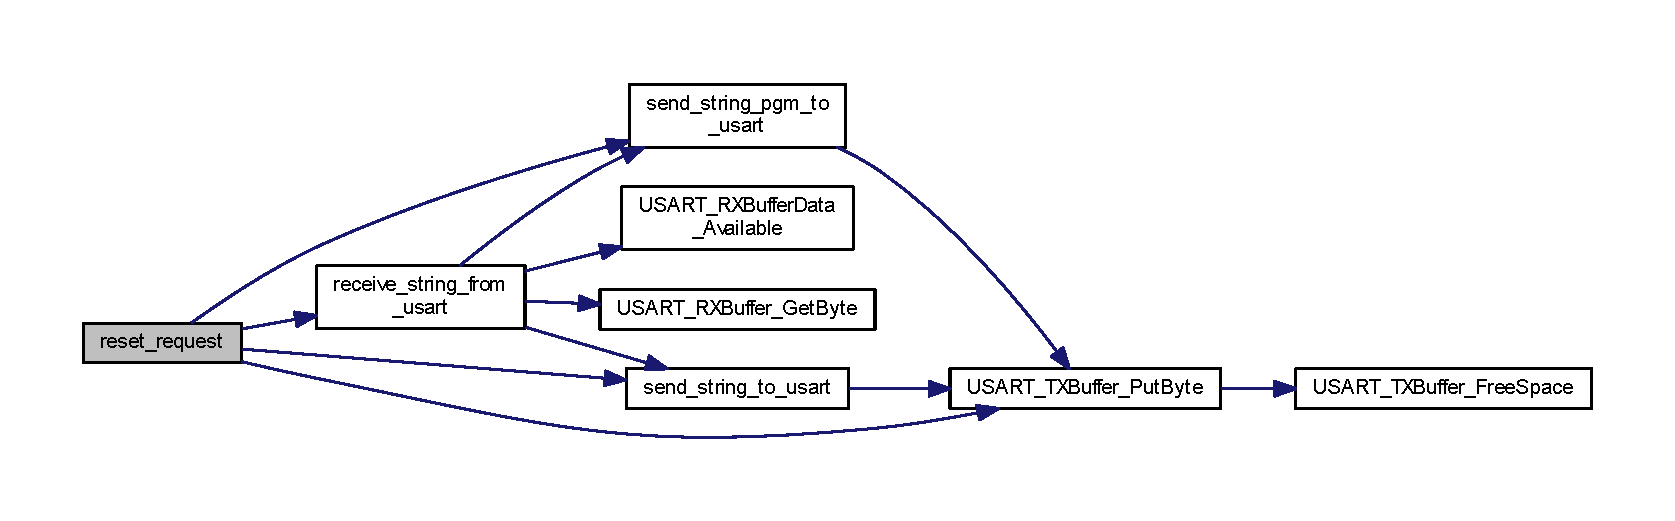
\includegraphics[width=350pt]{shell_8c_ab8aa91cc93dc57699d69cf98e7244d64_cgraph}
\end{center}
\end{figure}
Here is the caller graph for this function\+:
\nopagebreak
\begin{figure}[H]
\begin{center}
\leavevmode
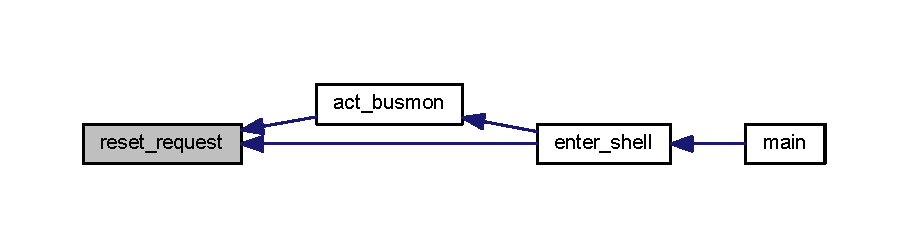
\includegraphics[width=350pt]{shell_8c_ab8aa91cc93dc57699d69cf98e7244d64_icgraph}
\end{center}
\end{figure}
\hypertarget{shell_8c_acd8340ade32d7f467cf3b625bd06ba31}{}\label{shell_8c_acd8340ade32d7f467cf3b625bd06ba31} 
\index{shell.\+c@{shell.\+c}!shell\+\_\+help@{shell\+\_\+help}}
\index{shell\+\_\+help@{shell\+\_\+help}!shell.\+c@{shell.\+c}}
\subsubsection{\texorpdfstring{shell\+\_\+help()}{shell\_help()}}
{\footnotesize\ttfamily void shell\+\_\+help (\begin{DoxyParamCaption}\item[{void}]{ }\end{DoxyParamCaption})}



Definition at line 334 of file shell.\+c.



References command, send\+\_\+string\+\_\+pgm\+\_\+to\+\_\+usart(), send\+\_\+string\+\_\+to\+\_\+usart(), and U\+S\+A\+R\+T\+\_\+\+D\+A\+T\+A\+\_\+\+PC.



Referenced by enter\+\_\+shell().

Here is the call graph for this function\+:
\nopagebreak
\begin{figure}[H]
\begin{center}
\leavevmode
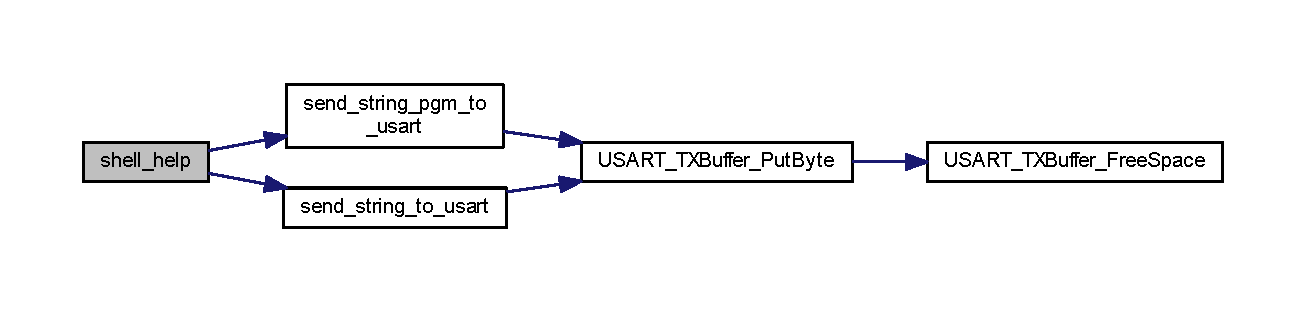
\includegraphics[width=350pt]{shell_8c_acd8340ade32d7f467cf3b625bd06ba31_cgraph}
\end{center}
\end{figure}
Here is the caller graph for this function\+:
\nopagebreak
\begin{figure}[H]
\begin{center}
\leavevmode
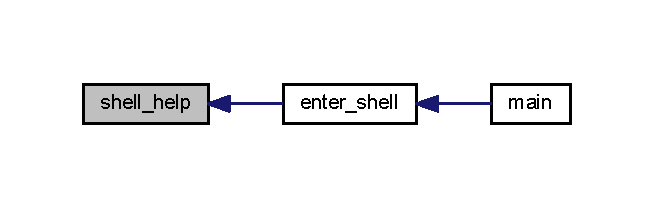
\includegraphics[width=314pt]{shell_8c_acd8340ade32d7f467cf3b625bd06ba31_icgraph}
\end{center}
\end{figure}
\hypertarget{shell_8c_a7e7bbbb940671ab75e317fb9e82e956d}{}\label{shell_8c_a7e7bbbb940671ab75e317fb9e82e956d} 
\index{shell.\+c@{shell.\+c}!state\+\_\+request@{state\+\_\+request}}
\index{state\+\_\+request@{state\+\_\+request}!shell.\+c@{shell.\+c}}
\subsubsection{\texorpdfstring{state\+\_\+request()}{state\_request()}}
{\footnotesize\ttfamily void state\+\_\+request (\begin{DoxyParamCaption}\item[{void}]{ }\end{DoxyParamCaption})}



Shell-\/\+Function for the U\+\_\+state.\+request-\/\+Service. 

Sends the U\+\_\+state.\+request to the T\+P\+U\+A\+RT and prints the Output as bits to the PC 

Definition at line 131 of file shell.\+c.



References command, receive\+\_\+string\+\_\+from\+\_\+usart(), send\+\_\+string\+\_\+pgm\+\_\+to\+\_\+usart(), send\+\_\+string\+\_\+to\+\_\+usart(), U\+S\+A\+R\+T\+\_\+\+D\+A\+T\+A\+\_\+\+PC, U\+S\+A\+R\+T\+\_\+\+D\+A\+T\+A\+\_\+\+TP, U\+S\+A\+R\+T\+\_\+\+R\+X\+\_\+\+B\+U\+F\+F\+E\+R\+\_\+\+S\+I\+ZE, and U\+S\+A\+R\+T\+\_\+\+T\+X\+Buffer\+\_\+\+Put\+Byte().



Referenced by enter\+\_\+shell().

Here is the call graph for this function\+:
\nopagebreak
\begin{figure}[H]
\begin{center}
\leavevmode
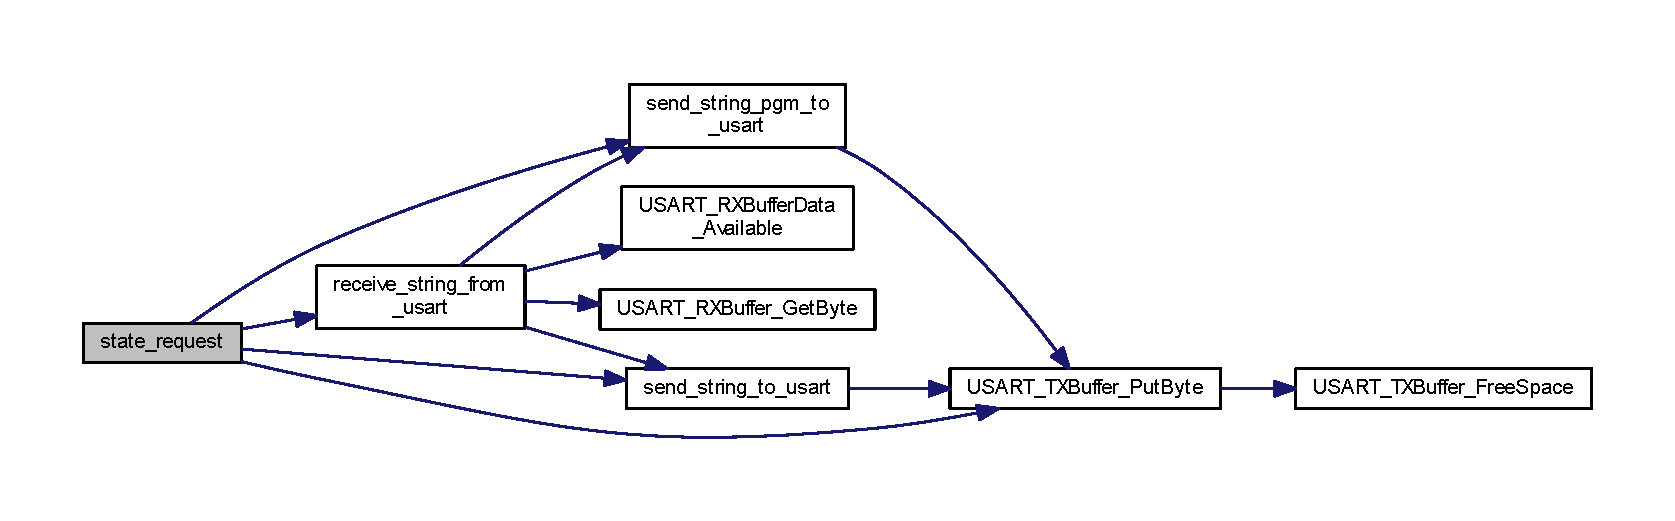
\includegraphics[width=350pt]{shell_8c_a7e7bbbb940671ab75e317fb9e82e956d_cgraph}
\end{center}
\end{figure}
Here is the caller graph for this function\+:
\nopagebreak
\begin{figure}[H]
\begin{center}
\leavevmode
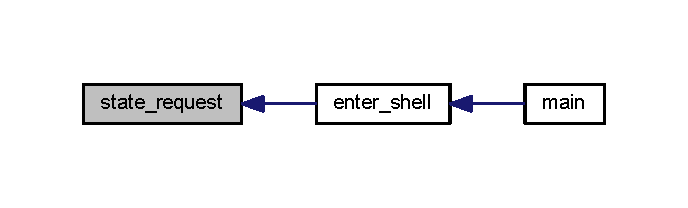
\includegraphics[width=330pt]{shell_8c_a7e7bbbb940671ab75e317fb9e82e956d_icgraph}
\end{center}
\end{figure}


\subsection{Variable Documentation}
\hypertarget{shell_8c_a68426a3f72e0fa2063f5140143c60965}{}\label{shell_8c_a68426a3f72e0fa2063f5140143c60965} 
\index{shell.\+c@{shell.\+c}!command@{command}}
\index{command@{command}!shell.\+c@{shell.\+c}}
\subsubsection{\texorpdfstring{command}{command}}
{\footnotesize\ttfamily char command\mbox{[}33\mbox{]}}



Definition at line 13 of file shell.\+c.



Referenced by act\+\_\+busmon(), act\+\_\+busymode(), enter\+\_\+shell(), prod\+\_\+request(), reset\+\_\+request(), shell\+\_\+help(), and state\+\_\+request().

\hypertarget{shell_8c_a37fd7702e47867237a1617ae4b4fab85}{}\label{shell_8c_a37fd7702e47867237a1617ae4b4fab85} 
\index{shell.\+c@{shell.\+c}!ret\+\_\+pressed@{ret\+\_\+pressed}}
\index{ret\+\_\+pressed@{ret\+\_\+pressed}!shell.\+c@{shell.\+c}}
\subsubsection{\texorpdfstring{ret\+\_\+pressed}{ret\_pressed}}
{\footnotesize\ttfamily int volatile ret\+\_\+pressed}



Definition at line 11 of file U\+A\+R\+T.\+c.



Referenced by enter\+\_\+shell(), and I\+S\+R().


\hypertarget{shell_8h}{}\section{shell.\+h File Reference}
\label{shell_8h}\index{shell.\+h@{shell.\+h}}


Corresponding header-\/\+File.  


{\ttfamily \#include \char`\"{}usart\+\_\+driver.\+h\char`\"{}}\newline
{\ttfamily \#include \char`\"{}avr\+\_\+compiler.\+h\char`\"{}}\newline
{\ttfamily \#include \char`\"{}U\+A\+R\+T.\+h\char`\"{}}\newline
{\ttfamily \#include $<$string.\+h$>$}\newline
Include dependency graph for shell.\+h\+:\nopagebreak
\begin{figure}[H]
\begin{center}
\leavevmode
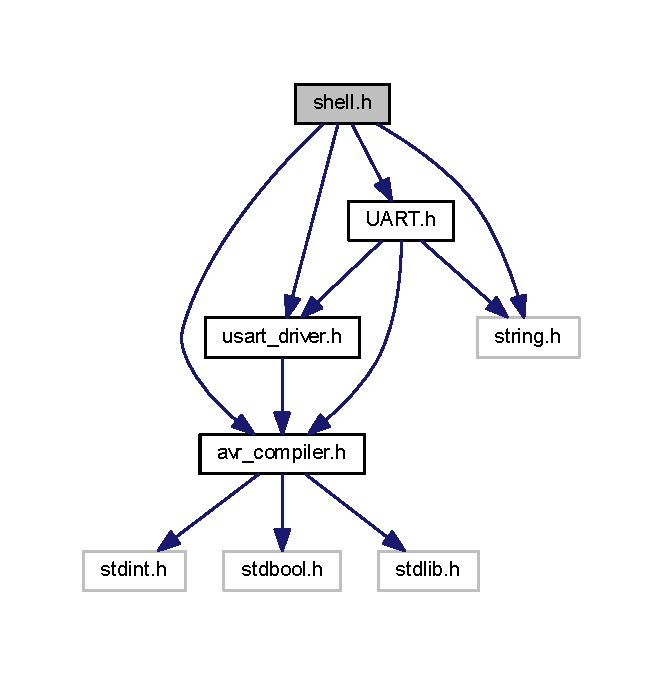
\includegraphics[width=318pt]{shell_8h__incl}
\end{center}
\end{figure}
This graph shows which files directly or indirectly include this file\+:
\nopagebreak
\begin{figure}[H]
\begin{center}
\leavevmode
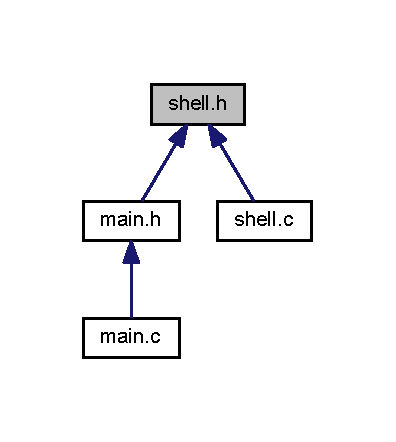
\includegraphics[width=190pt]{shell_8h__dep__incl}
\end{center}
\end{figure}
\subsection*{Functions}
\begin{DoxyCompactItemize}
\item 
void \hyperlink{shell_8h_a3197713442e02b97406567e4a11e193f}{enter\+\_\+shell} (\hyperlink{usart__driver_8h_a884c38d38327b0d4263c03cf0d84031e}{U\+S\+A\+R\+T\+\_\+data\+\_\+t} $\ast$U\+S\+A\+R\+T\+\_\+data)
\begin{DoxyCompactList}\small\item\em Enter the \char`\"{}\+Shell\char`\"{}. \end{DoxyCompactList}\item 
void \hyperlink{shell_8h_acd8340ade32d7f467cf3b625bd06ba31}{shell\+\_\+help} (void)
\item 
void \hyperlink{shell_8h_ab8aa91cc93dc57699d69cf98e7244d64}{reset\+\_\+request} (void)
\begin{DoxyCompactList}\small\item\em Shell-\/\+Function for the U\+\_\+reset.\+request-\/\+Service. \end{DoxyCompactList}\item 
void \hyperlink{shell_8h_a7e7bbbb940671ab75e317fb9e82e956d}{state\+\_\+request} (void)
\begin{DoxyCompactList}\small\item\em Shell-\/\+Function for the U\+\_\+state.\+request-\/\+Service. \end{DoxyCompactList}\item 
void \hyperlink{shell_8h_ad95c9c45c97cc744ca49a98494bf9465}{act\+\_\+busmon} (void)
\begin{DoxyCompactList}\small\item\em Shell-\/\+Function for the U\+\_\+\+Activate\+Busmon-\/\+Service. \end{DoxyCompactList}\item 
void \hyperlink{shell_8h_aef27926c3ebc8dc98a95df932af53a06}{prod\+\_\+request} (void)
\begin{DoxyCompactList}\small\item\em Shell-\/\+Function for the U\+\_\+\+Product\+I\+D.\+request-\/\+Service. \end{DoxyCompactList}\item 
void \hyperlink{shell_8h_a5c364cd022ec191bccd57afa8aae1e89}{act\+\_\+busymode} (void)
\begin{DoxyCompactList}\small\item\em Shell-\/\+Function for the U\+\_\+\+Activate\+Busy\+Mode. \end{DoxyCompactList}\end{DoxyCompactItemize}


\subsection{Detailed Description}
Corresponding header-\/\+File. 

\begin{DoxyAuthor}{Author}
Jan Baudis 
\end{DoxyAuthor}
\begin{DoxyDate}{Date}
03.\+12.\+2016 01\+:03\+:19 
\end{DoxyDate}


\subsection{Function Documentation}
\hypertarget{shell_8h_ad95c9c45c97cc744ca49a98494bf9465}{}\label{shell_8h_ad95c9c45c97cc744ca49a98494bf9465} 
\index{shell.\+h@{shell.\+h}!act\+\_\+busmon@{act\+\_\+busmon}}
\index{act\+\_\+busmon@{act\+\_\+busmon}!shell.\+h@{shell.\+h}}
\subsubsection{\texorpdfstring{act\+\_\+busmon()}{act\_busmon()}}
{\footnotesize\ttfamily void act\+\_\+busmon (\begin{DoxyParamCaption}\item[{void}]{ }\end{DoxyParamCaption})}



Shell-\/\+Function for the U\+\_\+\+Activate\+Busmon-\/\+Service. 

Sends the U\+\_\+\+Activate\+Busmon to the T\+P\+U\+A\+RT and prints the Output as bits to the PC. Listens till it receives any Key from the PC. Then it Resets the Chip since its the Only way to quit the Busmon-\/\+Mode of the T\+P\+U\+A\+RT.

\begin{DoxyRefDesc}{Todo}
\item[\hyperlink{todo__todo000002}{Todo}]Implement an end of Packet detection to print out some useful Information for the Bits.\end{DoxyRefDesc}


Definition at line 175 of file shell.\+c.



References command, flush\+\_\+\+U\+S\+A\+R\+T\+\_\+\+R\+X\+Buffer(), receive\+\_\+string\+\_\+from\+\_\+usart(), reset\+\_\+request(), send\+\_\+string\+\_\+pgm\+\_\+to\+\_\+usart(), send\+\_\+string\+\_\+to\+\_\+usart(), U\+S\+A\+R\+T\+\_\+\+D\+A\+T\+A\+\_\+\+PC, U\+S\+A\+R\+T\+\_\+\+D\+A\+T\+A\+\_\+\+TP, U\+S\+A\+R\+T\+\_\+\+R\+X\+\_\+\+B\+U\+F\+F\+E\+R\+\_\+\+S\+I\+ZE, U\+S\+A\+R\+T\+\_\+\+R\+X\+Buffer\+Data\+\_\+\+Available(), and U\+S\+A\+R\+T\+\_\+\+T\+X\+Buffer\+\_\+\+Put\+Byte().



Referenced by enter\+\_\+shell().

Here is the call graph for this function\+:
\nopagebreak
\begin{figure}[H]
\begin{center}
\leavevmode
\includegraphics[width=350pt]{shell_8h_ad95c9c45c97cc744ca49a98494bf9465_cgraph}
\end{center}
\end{figure}
Here is the caller graph for this function\+:
\nopagebreak
\begin{figure}[H]
\begin{center}
\leavevmode
\includegraphics[width=324pt]{shell_8h_ad95c9c45c97cc744ca49a98494bf9465_icgraph}
\end{center}
\end{figure}
\hypertarget{shell_8h_a5c364cd022ec191bccd57afa8aae1e89}{}\label{shell_8h_a5c364cd022ec191bccd57afa8aae1e89} 
\index{shell.\+h@{shell.\+h}!act\+\_\+busymode@{act\+\_\+busymode}}
\index{act\+\_\+busymode@{act\+\_\+busymode}!shell.\+h@{shell.\+h}}
\subsubsection{\texorpdfstring{act\+\_\+busymode()}{act\_busymode()}}
{\footnotesize\ttfamily void act\+\_\+busymode (\begin{DoxyParamCaption}\item[{void}]{ }\end{DoxyParamCaption})}



Shell-\/\+Function for the U\+\_\+\+Activate\+Busy\+Mode. 

Sends the U\+\_\+\+Activate\+Busy\+Mode to the T\+P\+U\+A\+RT and prints the Output as bits to the PC. T\+P-\/\+U\+A\+RT responses on every Packet which is addressed to him with B\+U\+SY within 700ms (+-\/10ms). All Packets are send to the Host and if the Host confirms one with U\+\_\+\+Ackinfo it will leave Busy\+Mode as well when reseted.

\begin{DoxyRefDesc}{Todo}
\item[\hyperlink{todo__todo000003}{Todo}]May add something; Dunno like a Listen Mode for 700ms; \end{DoxyRefDesc}


Definition at line 268 of file shell.\+c.



References command, prod\+\_\+request(), receive\+\_\+string\+\_\+from\+\_\+usart(), send\+\_\+string\+\_\+pgm\+\_\+to\+\_\+usart(), send\+\_\+string\+\_\+to\+\_\+usart(), U\+S\+A\+R\+T\+\_\+\+D\+A\+T\+A\+\_\+\+PC, U\+S\+A\+R\+T\+\_\+\+D\+A\+T\+A\+\_\+\+TP, U\+S\+A\+R\+T\+\_\+\+R\+X\+\_\+\+B\+U\+F\+F\+E\+R\+\_\+\+S\+I\+ZE, and U\+S\+A\+R\+T\+\_\+\+T\+X\+Buffer\+\_\+\+Put\+Byte().



Referenced by enter\+\_\+shell().

Here is the call graph for this function\+:
\nopagebreak
\begin{figure}[H]
\begin{center}
\leavevmode
\includegraphics[width=350pt]{shell_8h_a5c364cd022ec191bccd57afa8aae1e89_cgraph}
\end{center}
\end{figure}
Here is the caller graph for this function\+:
\nopagebreak
\begin{figure}[H]
\begin{center}
\leavevmode
\includegraphics[width=334pt]{shell_8h_a5c364cd022ec191bccd57afa8aae1e89_icgraph}
\end{center}
\end{figure}
\hypertarget{shell_8h_a3197713442e02b97406567e4a11e193f}{}\label{shell_8h_a3197713442e02b97406567e4a11e193f} 
\index{shell.\+h@{shell.\+h}!enter\+\_\+shell@{enter\+\_\+shell}}
\index{enter\+\_\+shell@{enter\+\_\+shell}!shell.\+h@{shell.\+h}}
\subsubsection{\texorpdfstring{enter\+\_\+shell()}{enter\_shell()}}
{\footnotesize\ttfamily void enter\+\_\+shell (\begin{DoxyParamCaption}\item[{\hyperlink{usart__driver_8h_a884c38d38327b0d4263c03cf0d84031e}{U\+S\+A\+R\+T\+\_\+data\+\_\+t} $\ast$}]{U\+S\+A\+R\+T\+\_\+data }\end{DoxyParamCaption})}



Enter the \char`\"{}\+Shell\char`\"{}. 

In the \char`\"{}\+Shell\char`\"{} we can e.\+g. use the Services of the T\+P\+U\+A\+RT


\begin{DoxyParams}{Parameters}
{\em U\+S\+A\+R\+T\+\_\+data} & The U\+S\+A\+R\+T\+\_\+data\+\_\+t struct instance. \\
\hline
\end{DoxyParams}


Definition at line 22 of file shell.\+c.



References act\+\_\+busmon(), act\+\_\+busymode(), command, prod\+\_\+request(), receive\+\_\+string\+\_\+from\+\_\+usart(), reset\+\_\+request(), ret\+\_\+pressed, send\+\_\+string\+\_\+pgm\+\_\+to\+\_\+usart(), send\+\_\+string\+\_\+to\+\_\+usart(), shell\+\_\+help(), state\+\_\+request(), and U\+S\+A\+R\+T\+\_\+\+D\+A\+T\+A\+\_\+\+PC.



Referenced by main().

Here is the call graph for this function\+:
\nopagebreak
\begin{figure}[H]
\begin{center}
\leavevmode
\includegraphics[width=350pt]{shell_8h_a3197713442e02b97406567e4a11e193f_cgraph}
\end{center}
\end{figure}
Here is the caller graph for this function\+:
\nopagebreak
\begin{figure}[H]
\begin{center}
\leavevmode
\includegraphics[width=218pt]{shell_8h_a3197713442e02b97406567e4a11e193f_icgraph}
\end{center}
\end{figure}
\hypertarget{shell_8h_aef27926c3ebc8dc98a95df932af53a06}{}\label{shell_8h_aef27926c3ebc8dc98a95df932af53a06} 
\index{shell.\+h@{shell.\+h}!prod\+\_\+request@{prod\+\_\+request}}
\index{prod\+\_\+request@{prod\+\_\+request}!shell.\+h@{shell.\+h}}
\subsubsection{\texorpdfstring{prod\+\_\+request()}{prod\_request()}}
{\footnotesize\ttfamily void prod\+\_\+request (\begin{DoxyParamCaption}\item[{void}]{ }\end{DoxyParamCaption})}



Shell-\/\+Function for the U\+\_\+\+Product\+I\+D.\+request-\/\+Service. 

Sends the U\+\_\+\+Product\+I\+D.\+request to the T\+P\+U\+A\+RT and prints the Output as bits to the PC 

Definition at line 224 of file shell.\+c.



References command, receive\+\_\+string\+\_\+from\+\_\+usart(), send\+\_\+string\+\_\+pgm\+\_\+to\+\_\+usart(), send\+\_\+string\+\_\+to\+\_\+usart(), U\+S\+A\+R\+T\+\_\+\+D\+A\+T\+A\+\_\+\+PC, U\+S\+A\+R\+T\+\_\+\+D\+A\+T\+A\+\_\+\+TP, U\+S\+A\+R\+T\+\_\+\+R\+X\+\_\+\+B\+U\+F\+F\+E\+R\+\_\+\+S\+I\+ZE, and U\+S\+A\+R\+T\+\_\+\+T\+X\+Buffer\+\_\+\+Put\+Byte().



Referenced by act\+\_\+busymode(), and enter\+\_\+shell().

Here is the call graph for this function\+:
\nopagebreak
\begin{figure}[H]
\begin{center}
\leavevmode
\includegraphics[width=350pt]{shell_8h_aef27926c3ebc8dc98a95df932af53a06_cgraph}
\end{center}
\end{figure}
Here is the caller graph for this function\+:
\nopagebreak
\begin{figure}[H]
\begin{center}
\leavevmode
\includegraphics[width=350pt]{shell_8h_aef27926c3ebc8dc98a95df932af53a06_icgraph}
\end{center}
\end{figure}
\hypertarget{shell_8h_ab8aa91cc93dc57699d69cf98e7244d64}{}\label{shell_8h_ab8aa91cc93dc57699d69cf98e7244d64} 
\index{shell.\+h@{shell.\+h}!reset\+\_\+request@{reset\+\_\+request}}
\index{reset\+\_\+request@{reset\+\_\+request}!shell.\+h@{shell.\+h}}
\subsubsection{\texorpdfstring{reset\+\_\+request()}{reset\_request()}}
{\footnotesize\ttfamily void reset\+\_\+request (\begin{DoxyParamCaption}\item[{void}]{ }\end{DoxyParamCaption})}



Shell-\/\+Function for the U\+\_\+reset.\+request-\/\+Service. 

Sends the U\+\_\+reset.\+request to the T\+P\+U\+A\+RT and prints the Output as bits to the PC 

Definition at line 89 of file shell.\+c.



References command, receive\+\_\+string\+\_\+from\+\_\+usart(), send\+\_\+string\+\_\+pgm\+\_\+to\+\_\+usart(), send\+\_\+string\+\_\+to\+\_\+usart(), U\+S\+A\+R\+T\+\_\+\+D\+A\+T\+A\+\_\+\+PC, U\+S\+A\+R\+T\+\_\+\+D\+A\+T\+A\+\_\+\+TP, U\+S\+A\+R\+T\+\_\+\+R\+X\+\_\+\+B\+U\+F\+F\+E\+R\+\_\+\+S\+I\+ZE, and U\+S\+A\+R\+T\+\_\+\+T\+X\+Buffer\+\_\+\+Put\+Byte().



Referenced by act\+\_\+busmon(), and enter\+\_\+shell().

Here is the call graph for this function\+:
\nopagebreak
\begin{figure}[H]
\begin{center}
\leavevmode
\includegraphics[width=350pt]{shell_8h_ab8aa91cc93dc57699d69cf98e7244d64_cgraph}
\end{center}
\end{figure}
Here is the caller graph for this function\+:
\nopagebreak
\begin{figure}[H]
\begin{center}
\leavevmode
\includegraphics[width=350pt]{shell_8h_ab8aa91cc93dc57699d69cf98e7244d64_icgraph}
\end{center}
\end{figure}
\hypertarget{shell_8h_acd8340ade32d7f467cf3b625bd06ba31}{}\label{shell_8h_acd8340ade32d7f467cf3b625bd06ba31} 
\index{shell.\+h@{shell.\+h}!shell\+\_\+help@{shell\+\_\+help}}
\index{shell\+\_\+help@{shell\+\_\+help}!shell.\+h@{shell.\+h}}
\subsubsection{\texorpdfstring{shell\+\_\+help()}{shell\_help()}}
{\footnotesize\ttfamily void shell\+\_\+help (\begin{DoxyParamCaption}\item[{void}]{ }\end{DoxyParamCaption})}



Definition at line 334 of file shell.\+c.



References command, send\+\_\+string\+\_\+pgm\+\_\+to\+\_\+usart(), send\+\_\+string\+\_\+to\+\_\+usart(), and U\+S\+A\+R\+T\+\_\+\+D\+A\+T\+A\+\_\+\+PC.



Referenced by enter\+\_\+shell().

Here is the call graph for this function\+:
\nopagebreak
\begin{figure}[H]
\begin{center}
\leavevmode
\includegraphics[width=350pt]{shell_8h_acd8340ade32d7f467cf3b625bd06ba31_cgraph}
\end{center}
\end{figure}
Here is the caller graph for this function\+:
\nopagebreak
\begin{figure}[H]
\begin{center}
\leavevmode
\includegraphics[width=314pt]{shell_8h_acd8340ade32d7f467cf3b625bd06ba31_icgraph}
\end{center}
\end{figure}
\hypertarget{shell_8h_a7e7bbbb940671ab75e317fb9e82e956d}{}\label{shell_8h_a7e7bbbb940671ab75e317fb9e82e956d} 
\index{shell.\+h@{shell.\+h}!state\+\_\+request@{state\+\_\+request}}
\index{state\+\_\+request@{state\+\_\+request}!shell.\+h@{shell.\+h}}
\subsubsection{\texorpdfstring{state\+\_\+request()}{state\_request()}}
{\footnotesize\ttfamily void state\+\_\+request (\begin{DoxyParamCaption}\item[{void}]{ }\end{DoxyParamCaption})}



Shell-\/\+Function for the U\+\_\+state.\+request-\/\+Service. 

Sends the U\+\_\+state.\+request to the T\+P\+U\+A\+RT and prints the Output as bits to the PC 

Definition at line 131 of file shell.\+c.



References command, receive\+\_\+string\+\_\+from\+\_\+usart(), send\+\_\+string\+\_\+pgm\+\_\+to\+\_\+usart(), send\+\_\+string\+\_\+to\+\_\+usart(), U\+S\+A\+R\+T\+\_\+\+D\+A\+T\+A\+\_\+\+PC, U\+S\+A\+R\+T\+\_\+\+D\+A\+T\+A\+\_\+\+TP, U\+S\+A\+R\+T\+\_\+\+R\+X\+\_\+\+B\+U\+F\+F\+E\+R\+\_\+\+S\+I\+ZE, and U\+S\+A\+R\+T\+\_\+\+T\+X\+Buffer\+\_\+\+Put\+Byte().



Referenced by enter\+\_\+shell().

Here is the call graph for this function\+:
\nopagebreak
\begin{figure}[H]
\begin{center}
\leavevmode
\includegraphics[width=350pt]{shell_8h_a7e7bbbb940671ab75e317fb9e82e956d_cgraph}
\end{center}
\end{figure}
Here is the caller graph for this function\+:
\nopagebreak
\begin{figure}[H]
\begin{center}
\leavevmode
\includegraphics[width=330pt]{shell_8h_a7e7bbbb940671ab75e317fb9e82e956d_icgraph}
\end{center}
\end{figure}

\hypertarget{_u_a_r_t_8c}{}\section{U\+A\+R\+T.\+c File Reference}
\label{_u_a_r_t_8c}\index{U\+A\+R\+T.\+c@{U\+A\+R\+T.\+c}}


This file contains the Basic Functions to use the interrupt driven U\+S\+A\+RT Driver provided by Atmel and it sets the I\+S\+Rs Many things taken from the usart\+\_\+example\+\_\+interrupt.\+c-\/\+File provided by Atmel.  


{\ttfamily \#include \char`\"{}U\+A\+R\+T.\+h\char`\"{}}\newline
Include dependency graph for U\+A\+R\+T.\+c\+:\nopagebreak
\begin{figure}[H]
\begin{center}
\leavevmode
\includegraphics[width=286pt]{_u_a_r_t_8c__incl}
\end{center}
\end{figure}
\subsection*{Functions}
\begin{DoxyCompactItemize}
\item 
void \hyperlink{_u_a_r_t_8c_a09e438e4f709b00836cebb0d6a44f223}{usart\+\_\+init\+\_\+tpuart} (void)
\begin{DoxyCompactList}\small\item\em This Method enables and initializes the U\+S\+A\+RT for the specific purpose to communicate with the T\+P\+U\+A\+R\+T1 Chip. \end{DoxyCompactList}\item 
void \hyperlink{_u_a_r_t_8c_a267c0b0bf7f4f8b70049d91449590cf8}{usart\+\_\+init\+\_\+pc} (void)
\begin{DoxyCompactList}\small\item\em This Method enables and initializes the U\+S\+A\+RT for the specific purpose to communicate with e.\+g. a PC. \end{DoxyCompactList}\item 
void \hyperlink{_u_a_r_t_8c_ad7bb1da26c447116e627aef512f5fc84}{send\+\_\+string\+\_\+pgm\+\_\+to\+\_\+usart} (\hyperlink{usart__driver_8h_a884c38d38327b0d4263c03cf0d84031e}{U\+S\+A\+R\+T\+\_\+data\+\_\+t} $\ast$U\+S\+A\+R\+T\+\_\+data, const char $\ast$addr)
\begin{DoxyCompactList}\small\item\em This Method uses the Program Space for e.\+g. Debug Strings and sends them to the given U\+S\+A\+RT. \end{DoxyCompactList}\item 
void \hyperlink{_u_a_r_t_8c_a190114969cf3d32ab5e83509d7ab1569}{send\+\_\+string\+\_\+to\+\_\+usart} (\hyperlink{usart__driver_8h_a884c38d38327b0d4263c03cf0d84031e}{U\+S\+A\+R\+T\+\_\+data\+\_\+t} $\ast$U\+S\+A\+R\+T\+\_\+data, char $\ast$s)
\begin{DoxyCompactList}\small\item\em This Method sends Strings to the given U\+S\+A\+RT. \end{DoxyCompactList}\item 
void \hyperlink{_u_a_r_t_8c_abae42fc5d4a757188ac79c5d6ecf34be}{receive\+\_\+string\+\_\+from\+\_\+usart} (\hyperlink{usart__driver_8h_a884c38d38327b0d4263c03cf0d84031e}{U\+S\+A\+R\+T\+\_\+data\+\_\+t} $\ast$U\+S\+A\+R\+T\+\_\+data, char $\ast$output)
\begin{DoxyCompactList}\small\item\em This Method reads out the data of the Ring\+Buffer and returns a string. \end{DoxyCompactList}\item 
char \hyperlink{_u_a_r_t_8c_a1937cef99bb4eb8ca37fd7b128750c1b}{receive\+\_\+char\+\_\+from\+\_\+usart} (\hyperlink{usart__driver_8h_a884c38d38327b0d4263c03cf0d84031e}{U\+S\+A\+R\+T\+\_\+data\+\_\+t} $\ast$U\+S\+A\+R\+T\+\_\+data)
\begin{DoxyCompactList}\small\item\em This Method waits till one char is in the given U\+S\+A\+R\+T-\/\+Buffer -\/ No Timeout, Blocks!!!!. \end{DoxyCompactList}\item 
void \hyperlink{_u_a_r_t_8c_a6c34e7e2146aab25f22bf042eae221ac}{flush\+\_\+\+U\+S\+A\+R\+T\+\_\+\+R\+X\+Buffer} (\hyperlink{usart__driver_8h_a884c38d38327b0d4263c03cf0d84031e}{U\+S\+A\+R\+T\+\_\+data\+\_\+t} $\ast$U\+S\+A\+R\+T\+\_\+data)
\begin{DoxyCompactList}\small\item\em This Method flushs the RX Buffer. \end{DoxyCompactList}\item 
\hyperlink{_u_a_r_t_8c_aace195abde7bc36b7b50772ff2277dd4}{I\+SR} (U\+S\+A\+R\+T\+C0\+\_\+\+R\+X\+C\+\_\+vect)
\begin{DoxyCompactList}\small\item\em Receive complete interrupt service routine. \end{DoxyCompactList}\item 
\hyperlink{_u_a_r_t_8c_abbfd0611f43db59ea4fdb1ea434cf017}{I\+SR} (U\+S\+A\+R\+T\+C0\+\_\+\+D\+R\+E\+\_\+vect)
\begin{DoxyCompactList}\small\item\em Data register empty interrupt service routine. \end{DoxyCompactList}\item 
\hyperlink{_u_a_r_t_8c_a6c9949e5146d1feb028b0c2db8754523}{I\+SR} (U\+S\+A\+R\+T\+C1\+\_\+\+R\+X\+C\+\_\+vect)
\begin{DoxyCompactList}\small\item\em Receive complete interrupt service routine. \end{DoxyCompactList}\item 
\hyperlink{_u_a_r_t_8c_acdf978f69a52b8a2225b0536b5fbff0e}{I\+SR} (U\+S\+A\+R\+T\+C1\+\_\+\+D\+R\+E\+\_\+vect)
\begin{DoxyCompactList}\small\item\em Data register empty interrupt service routine. \end{DoxyCompactList}\end{DoxyCompactItemize}
\subsection*{Variables}
\begin{DoxyCompactItemize}
\item 
volatile int \hyperlink{_u_a_r_t_8c_a27f65714e943ab0e7014f4fff8e2d833}{ret\+\_\+pressed} = 0
\end{DoxyCompactItemize}


\subsection{Detailed Description}
This file contains the Basic Functions to use the interrupt driven U\+S\+A\+RT Driver provided by Atmel and it sets the I\+S\+Rs Many things taken from the usart\+\_\+example\+\_\+interrupt.\+c-\/\+File provided by Atmel. 

\begin{DoxyAuthor}{Author}
Jan Baudis 
\end{DoxyAuthor}
\begin{DoxyDate}{Date}
13.\+09.\+2016 16\+:17\+:44 
\end{DoxyDate}
\begin{DoxyRefDesc}{Todo}
\item[\hyperlink{todo__todo000004}{Todo}]Change the U\+A\+R\+T-\/\+Functions -\/ add an extra value for the Port used and not an simple string to select it in the Function for both Init Functions \end{DoxyRefDesc}


\subsection{Function Documentation}
\hypertarget{_u_a_r_t_8c_a6c34e7e2146aab25f22bf042eae221ac}{}\label{_u_a_r_t_8c_a6c34e7e2146aab25f22bf042eae221ac} 
\index{U\+A\+R\+T.\+c@{U\+A\+R\+T.\+c}!flush\+\_\+\+U\+S\+A\+R\+T\+\_\+\+R\+X\+Buffer@{flush\+\_\+\+U\+S\+A\+R\+T\+\_\+\+R\+X\+Buffer}}
\index{flush\+\_\+\+U\+S\+A\+R\+T\+\_\+\+R\+X\+Buffer@{flush\+\_\+\+U\+S\+A\+R\+T\+\_\+\+R\+X\+Buffer}!U\+A\+R\+T.\+c@{U\+A\+R\+T.\+c}}
\subsubsection{\texorpdfstring{flush\+\_\+\+U\+S\+A\+R\+T\+\_\+\+R\+X\+Buffer()}{flush\_USART\_RXBuffer()}}
{\footnotesize\ttfamily void flush\+\_\+\+U\+S\+A\+R\+T\+\_\+\+R\+X\+Buffer (\begin{DoxyParamCaption}\item[{\hyperlink{usart__driver_8h_a884c38d38327b0d4263c03cf0d84031e}{U\+S\+A\+R\+T\+\_\+data\+\_\+t} $\ast$}]{U\+S\+A\+R\+T\+\_\+data }\end{DoxyParamCaption})}



This Method flushs the RX Buffer. 


\begin{DoxyParams}{Parameters}
{\em U\+S\+A\+R\+T\+\_\+data} & The U\+S\+A\+R\+T\+\_\+data\+\_\+t struct instance. \\
\hline
\end{DoxyParams}


Definition at line 198 of file U\+A\+R\+T.\+c.



References send\+\_\+string\+\_\+pgm\+\_\+to\+\_\+usart(), U\+S\+A\+R\+T\+\_\+\+D\+A\+T\+A\+\_\+\+PC, U\+S\+A\+R\+T\+\_\+\+R\+X\+Buffer\+\_\+\+Get\+Byte(), and U\+S\+A\+R\+T\+\_\+\+R\+X\+Buffer\+Data\+\_\+\+Available().



Referenced by act\+\_\+busmon().

Here is the call graph for this function\+:\nopagebreak
\begin{figure}[H]
\begin{center}
\leavevmode
\includegraphics[width=350pt]{_u_a_r_t_8c_a6c34e7e2146aab25f22bf042eae221ac_cgraph}
\end{center}
\end{figure}
Here is the caller graph for this function\+:\nopagebreak
\begin{figure}[H]
\begin{center}
\leavevmode
\includegraphics[width=350pt]{_u_a_r_t_8c_a6c34e7e2146aab25f22bf042eae221ac_icgraph}
\end{center}
\end{figure}
\hypertarget{_u_a_r_t_8c_aace195abde7bc36b7b50772ff2277dd4}{}\label{_u_a_r_t_8c_aace195abde7bc36b7b50772ff2277dd4} 
\index{U\+A\+R\+T.\+c@{U\+A\+R\+T.\+c}!I\+SR@{I\+SR}}
\index{I\+SR@{I\+SR}!U\+A\+R\+T.\+c@{U\+A\+R\+T.\+c}}
\subsubsection{\texorpdfstring{I\+S\+R()}{ISR()}\hspace{0.1cm}{\footnotesize\ttfamily [1/4]}}
{\footnotesize\ttfamily I\+SR (\begin{DoxyParamCaption}\item[{U\+S\+A\+R\+T\+C0\+\_\+\+R\+X\+C\+\_\+vect}]{ }\end{DoxyParamCaption})}



Receive complete interrupt service routine. 

Receive complete interrupt service routine. Calls the common receive complete handler with pointer to the correct U\+S\+A\+RT as argument.

\begin{DoxyRefDesc}{Todo}
\item[\hyperlink{todo__todo000007}{Todo}]Think about if volatile for the U\+S\+A\+R\+T\+\_\+\+D\+A\+T\+A\+\_\+\+TP is needed!\end{DoxyRefDesc}


Definition at line 224 of file U\+A\+R\+T.\+c.



References U\+S\+A\+R\+T\+\_\+\+D\+A\+T\+A\+\_\+\+TP, and U\+S\+A\+R\+T\+\_\+\+R\+X\+Complete().

Here is the call graph for this function\+:\nopagebreak
\begin{figure}[H]
\begin{center}
\leavevmode
\includegraphics[width=255pt]{_u_a_r_t_8c_aace195abde7bc36b7b50772ff2277dd4_cgraph}
\end{center}
\end{figure}
\hypertarget{_u_a_r_t_8c_abbfd0611f43db59ea4fdb1ea434cf017}{}\label{_u_a_r_t_8c_abbfd0611f43db59ea4fdb1ea434cf017} 
\index{U\+A\+R\+T.\+c@{U\+A\+R\+T.\+c}!I\+SR@{I\+SR}}
\index{I\+SR@{I\+SR}!U\+A\+R\+T.\+c@{U\+A\+R\+T.\+c}}
\subsubsection{\texorpdfstring{I\+S\+R()}{ISR()}\hspace{0.1cm}{\footnotesize\ttfamily [2/4]}}
{\footnotesize\ttfamily I\+SR (\begin{DoxyParamCaption}\item[{U\+S\+A\+R\+T\+C0\+\_\+\+D\+R\+E\+\_\+vect}]{ }\end{DoxyParamCaption})}



Data register empty interrupt service routine. 

Data register empty interrupt service routine. Calls the common data register empty complete handler with pointer to the correct U\+S\+A\+RT as argument.

\begin{DoxyRefDesc}{Todo}
\item[\hyperlink{todo__todo000008}{Todo}]Think about if volatile for the U\+S\+A\+R\+T\+\_\+\+D\+A\+T\+A\+\_\+\+TP is needed!\end{DoxyRefDesc}


Definition at line 239 of file U\+A\+R\+T.\+c.



References U\+S\+A\+R\+T\+\_\+\+D\+A\+T\+A\+\_\+\+TP, and U\+S\+A\+R\+T\+\_\+\+Data\+Reg\+Empty().

Here is the call graph for this function\+:\nopagebreak
\begin{figure}[H]
\begin{center}
\leavevmode
\includegraphics[width=268pt]{_u_a_r_t_8c_abbfd0611f43db59ea4fdb1ea434cf017_cgraph}
\end{center}
\end{figure}
\hypertarget{_u_a_r_t_8c_a6c9949e5146d1feb028b0c2db8754523}{}\label{_u_a_r_t_8c_a6c9949e5146d1feb028b0c2db8754523} 
\index{U\+A\+R\+T.\+c@{U\+A\+R\+T.\+c}!I\+SR@{I\+SR}}
\index{I\+SR@{I\+SR}!U\+A\+R\+T.\+c@{U\+A\+R\+T.\+c}}
\subsubsection{\texorpdfstring{I\+S\+R()}{ISR()}\hspace{0.1cm}{\footnotesize\ttfamily [3/4]}}
{\footnotesize\ttfamily I\+SR (\begin{DoxyParamCaption}\item[{U\+S\+A\+R\+T\+C1\+\_\+\+R\+X\+C\+\_\+vect}]{ }\end{DoxyParamCaption})}



Receive complete interrupt service routine. 

Receive complete interrupt service routine. Calls the common receive complete handler with pointer to the correct U\+S\+A\+RT as argument.

\begin{DoxyRefDesc}{Todo}
\item[\hyperlink{todo__todo000009}{Todo}]Think about if volatile for the U\+S\+A\+R\+T\+\_\+\+D\+A\+T\+A\+\_\+\+PC is needed! \end{DoxyRefDesc}
\begin{DoxyNote}{Note}
Added a check to see if the Return-\/\+Key was pressed to trigger the \char`\"{}\+Shell\char`\"{} 
\end{DoxyNote}
If it receives the Return-\/\+Key(13) it changes ret\+\_\+pressed so the Shell can evalute the command 

Definition at line 254 of file U\+A\+R\+T.\+c.



References Usart\+\_\+and\+\_\+buffer\+::buffer, ret\+\_\+pressed, U\+S\+A\+R\+T\+\_\+\+Buffer\+::\+RX, U\+S\+A\+R\+T\+\_\+\+Buffer\+::\+R\+X\+\_\+\+Head, U\+S\+A\+R\+T\+\_\+data\+\_\+c1, U\+S\+A\+R\+T\+\_\+\+D\+A\+T\+A\+\_\+\+PC, U\+S\+A\+R\+T\+\_\+\+R\+X\+\_\+\+B\+U\+F\+F\+E\+R\+\_\+\+M\+A\+SK, and U\+S\+A\+R\+T\+\_\+\+R\+X\+Complete().

Here is the call graph for this function\+:\nopagebreak
\begin{figure}[H]
\begin{center}
\leavevmode
\includegraphics[width=255pt]{_u_a_r_t_8c_a6c9949e5146d1feb028b0c2db8754523_cgraph}
\end{center}
\end{figure}
\hypertarget{_u_a_r_t_8c_acdf978f69a52b8a2225b0536b5fbff0e}{}\label{_u_a_r_t_8c_acdf978f69a52b8a2225b0536b5fbff0e} 
\index{U\+A\+R\+T.\+c@{U\+A\+R\+T.\+c}!I\+SR@{I\+SR}}
\index{I\+SR@{I\+SR}!U\+A\+R\+T.\+c@{U\+A\+R\+T.\+c}}
\subsubsection{\texorpdfstring{I\+S\+R()}{ISR()}\hspace{0.1cm}{\footnotesize\ttfamily [4/4]}}
{\footnotesize\ttfamily I\+SR (\begin{DoxyParamCaption}\item[{U\+S\+A\+R\+T\+C1\+\_\+\+D\+R\+E\+\_\+vect}]{ }\end{DoxyParamCaption})}



Data register empty interrupt service routine. 

Data register empty interrupt service routine. Calls the common data register empty complete handler with pointer to the correct U\+S\+A\+RT as argument.

\begin{DoxyRefDesc}{Todo}
\item[\hyperlink{todo__todo000010}{Todo}]Think about if volatile for the U\+S\+A\+R\+T\+\_\+\+D\+A\+T\+A\+\_\+\+PC is needed!\end{DoxyRefDesc}


Definition at line 274 of file U\+A\+R\+T.\+c.



References U\+S\+A\+R\+T\+\_\+\+D\+A\+T\+A\+\_\+\+PC, and U\+S\+A\+R\+T\+\_\+\+Data\+Reg\+Empty().

Here is the call graph for this function\+:\nopagebreak
\begin{figure}[H]
\begin{center}
\leavevmode
\includegraphics[width=268pt]{_u_a_r_t_8c_acdf978f69a52b8a2225b0536b5fbff0e_cgraph}
\end{center}
\end{figure}
\hypertarget{_u_a_r_t_8c_a1937cef99bb4eb8ca37fd7b128750c1b}{}\label{_u_a_r_t_8c_a1937cef99bb4eb8ca37fd7b128750c1b} 
\index{U\+A\+R\+T.\+c@{U\+A\+R\+T.\+c}!receive\+\_\+char\+\_\+from\+\_\+usart@{receive\+\_\+char\+\_\+from\+\_\+usart}}
\index{receive\+\_\+char\+\_\+from\+\_\+usart@{receive\+\_\+char\+\_\+from\+\_\+usart}!U\+A\+R\+T.\+c@{U\+A\+R\+T.\+c}}
\subsubsection{\texorpdfstring{receive\+\_\+char\+\_\+from\+\_\+usart()}{receive\_char\_from\_usart()}}
{\footnotesize\ttfamily char receive\+\_\+char\+\_\+from\+\_\+usart (\begin{DoxyParamCaption}\item[{\hyperlink{usart__driver_8h_a884c38d38327b0d4263c03cf0d84031e}{U\+S\+A\+R\+T\+\_\+data\+\_\+t} $\ast$}]{U\+S\+A\+R\+T\+\_\+data }\end{DoxyParamCaption})}



This Method waits till one char is in the given U\+S\+A\+R\+T-\/\+Buffer -\/ No Timeout, Blocks!!!!. 


\begin{DoxyParams}{Parameters}
{\em U\+S\+A\+R\+T\+\_\+data} & The U\+S\+A\+R\+T\+\_\+data\+\_\+t struct instance. \\
\hline
\end{DoxyParams}


Definition at line 175 of file U\+A\+R\+T.\+c.



References send\+\_\+string\+\_\+pgm\+\_\+to\+\_\+usart(), U\+S\+A\+R\+T\+\_\+\+D\+A\+T\+A\+\_\+\+PC, U\+S\+A\+R\+T\+\_\+\+R\+X\+Buffer\+\_\+\+Get\+Byte(), and U\+S\+A\+R\+T\+\_\+\+R\+X\+Buffer\+Data\+\_\+\+Available().

Here is the call graph for this function\+:\nopagebreak
\begin{figure}[H]
\begin{center}
\leavevmode
\includegraphics[width=350pt]{_u_a_r_t_8c_a1937cef99bb4eb8ca37fd7b128750c1b_cgraph}
\end{center}
\end{figure}
\hypertarget{_u_a_r_t_8c_abae42fc5d4a757188ac79c5d6ecf34be}{}\label{_u_a_r_t_8c_abae42fc5d4a757188ac79c5d6ecf34be} 
\index{U\+A\+R\+T.\+c@{U\+A\+R\+T.\+c}!receive\+\_\+string\+\_\+from\+\_\+usart@{receive\+\_\+string\+\_\+from\+\_\+usart}}
\index{receive\+\_\+string\+\_\+from\+\_\+usart@{receive\+\_\+string\+\_\+from\+\_\+usart}!U\+A\+R\+T.\+c@{U\+A\+R\+T.\+c}}
\subsubsection{\texorpdfstring{receive\+\_\+string\+\_\+from\+\_\+usart()}{receive\_string\_from\_usart()}}
{\footnotesize\ttfamily void receive\+\_\+string\+\_\+from\+\_\+usart (\begin{DoxyParamCaption}\item[{\hyperlink{usart__driver_8h_a884c38d38327b0d4263c03cf0d84031e}{U\+S\+A\+R\+T\+\_\+data\+\_\+t} $\ast$}]{U\+S\+A\+R\+T\+\_\+data,  }\item[{char $\ast$}]{output }\end{DoxyParamCaption})}



This Method reads out the data of the Ring\+Buffer and returns a string. 


\begin{DoxyParams}{Parameters}
{\em U\+S\+A\+R\+T\+\_\+data} & The U\+S\+A\+R\+T\+\_\+data\+\_\+t struct instance. \\
\hline
{\em output} & The String-\/\+Pointer where the Output is stored \\
\hline
\end{DoxyParams}


Definition at line 148 of file U\+A\+R\+T.\+c.



References send\+\_\+string\+\_\+pgm\+\_\+to\+\_\+usart(), send\+\_\+string\+\_\+to\+\_\+usart(), U\+S\+A\+R\+T\+\_\+\+D\+A\+T\+A\+\_\+\+PC, U\+S\+A\+R\+T\+\_\+\+R\+X\+Buffer\+\_\+\+Get\+Byte(), and U\+S\+A\+R\+T\+\_\+\+R\+X\+Buffer\+Data\+\_\+\+Available().



Referenced by act\+\_\+busmon(), act\+\_\+busymode(), enter\+\_\+shell(), main(), prod\+\_\+request(), reset\+\_\+request(), and state\+\_\+request().

Here is the call graph for this function\+:\nopagebreak
\begin{figure}[H]
\begin{center}
\leavevmode
\includegraphics[width=350pt]{_u_a_r_t_8c_abae42fc5d4a757188ac79c5d6ecf34be_cgraph}
\end{center}
\end{figure}
Here is the caller graph for this function\+:
\nopagebreak
\begin{figure}[H]
\begin{center}
\leavevmode
\includegraphics[width=350pt]{_u_a_r_t_8c_abae42fc5d4a757188ac79c5d6ecf34be_icgraph}
\end{center}
\end{figure}
\hypertarget{_u_a_r_t_8c_ad7bb1da26c447116e627aef512f5fc84}{}\label{_u_a_r_t_8c_ad7bb1da26c447116e627aef512f5fc84} 
\index{U\+A\+R\+T.\+c@{U\+A\+R\+T.\+c}!send\+\_\+string\+\_\+pgm\+\_\+to\+\_\+usart@{send\+\_\+string\+\_\+pgm\+\_\+to\+\_\+usart}}
\index{send\+\_\+string\+\_\+pgm\+\_\+to\+\_\+usart@{send\+\_\+string\+\_\+pgm\+\_\+to\+\_\+usart}!U\+A\+R\+T.\+c@{U\+A\+R\+T.\+c}}
\subsubsection{\texorpdfstring{send\+\_\+string\+\_\+pgm\+\_\+to\+\_\+usart()}{send\_string\_pgm\_to\_usart()}}
{\footnotesize\ttfamily void send\+\_\+string\+\_\+pgm\+\_\+to\+\_\+usart (\begin{DoxyParamCaption}\item[{\hyperlink{usart__driver_8h_a884c38d38327b0d4263c03cf0d84031e}{U\+S\+A\+R\+T\+\_\+data\+\_\+t} $\ast$}]{U\+S\+A\+R\+T\+\_\+data,  }\item[{const char $\ast$}]{addr }\end{DoxyParamCaption})}



This Method uses the Program Space for e.\+g. Debug Strings and sends them to the given U\+S\+A\+RT. 


\begin{DoxyParams}{Parameters}
{\em U\+S\+A\+R\+T\+\_\+data} & The U\+S\+A\+R\+T\+\_\+data\+\_\+t struct instance. \\
\hline
{\em addr} & const char$\ast$ to the pgmspace. \\
\hline
\end{DoxyParams}


Definition at line 107 of file U\+A\+R\+T.\+c.



References U\+S\+A\+R\+T\+\_\+\+T\+X\+Buffer\+\_\+\+Put\+Byte().



Referenced by act\+\_\+busmon(), act\+\_\+busymode(), enter\+\_\+shell(), flush\+\_\+\+U\+S\+A\+R\+T\+\_\+\+R\+X\+Buffer(), main(), prod\+\_\+request(), receive\+\_\+char\+\_\+from\+\_\+usart(), receive\+\_\+string\+\_\+from\+\_\+usart(), reset\+\_\+request(), shell\+\_\+help(), and state\+\_\+request().

Here is the call graph for this function\+:
\nopagebreak
\begin{figure}[H]
\begin{center}
\leavevmode
\includegraphics[width=350pt]{_u_a_r_t_8c_ad7bb1da26c447116e627aef512f5fc84_cgraph}
\end{center}
\end{figure}
Here is the caller graph for this function\+:
\nopagebreak
\begin{figure}[H]
\begin{center}
\leavevmode
\includegraphics[width=350pt]{_u_a_r_t_8c_ad7bb1da26c447116e627aef512f5fc84_icgraph}
\end{center}
\end{figure}
\hypertarget{_u_a_r_t_8c_a190114969cf3d32ab5e83509d7ab1569}{}\label{_u_a_r_t_8c_a190114969cf3d32ab5e83509d7ab1569} 
\index{U\+A\+R\+T.\+c@{U\+A\+R\+T.\+c}!send\+\_\+string\+\_\+to\+\_\+usart@{send\+\_\+string\+\_\+to\+\_\+usart}}
\index{send\+\_\+string\+\_\+to\+\_\+usart@{send\+\_\+string\+\_\+to\+\_\+usart}!U\+A\+R\+T.\+c@{U\+A\+R\+T.\+c}}
\subsubsection{\texorpdfstring{send\+\_\+string\+\_\+to\+\_\+usart()}{send\_string\_to\_usart()}}
{\footnotesize\ttfamily void send\+\_\+string\+\_\+to\+\_\+usart (\begin{DoxyParamCaption}\item[{\hyperlink{usart__driver_8h_a884c38d38327b0d4263c03cf0d84031e}{U\+S\+A\+R\+T\+\_\+data\+\_\+t} $\ast$}]{U\+S\+A\+R\+T\+\_\+data,  }\item[{char $\ast$}]{s }\end{DoxyParamCaption})}



This Method sends Strings to the given U\+S\+A\+RT. 


\begin{DoxyParams}{Parameters}
{\em U\+S\+A\+R\+T\+\_\+data} & The U\+S\+A\+R\+T\+\_\+data\+\_\+t struct instance. \\
\hline
{\em s} & char$\ast$ to transmit. \\
\hline
\end{DoxyParams}


Definition at line 129 of file U\+A\+R\+T.\+c.



References U\+S\+A\+R\+T\+\_\+\+T\+X\+Buffer\+\_\+\+Put\+Byte().



Referenced by act\+\_\+busmon(), act\+\_\+busymode(), enter\+\_\+shell(), main(), prod\+\_\+request(), receive\+\_\+string\+\_\+from\+\_\+usart(), reset\+\_\+request(), shell\+\_\+help(), and state\+\_\+request().

Here is the call graph for this function\+:
\nopagebreak
\begin{figure}[H]
\begin{center}
\leavevmode
\includegraphics[width=350pt]{_u_a_r_t_8c_a190114969cf3d32ab5e83509d7ab1569_cgraph}
\end{center}
\end{figure}
Here is the caller graph for this function\+:
\nopagebreak
\begin{figure}[H]
\begin{center}
\leavevmode
\includegraphics[width=350pt]{_u_a_r_t_8c_a190114969cf3d32ab5e83509d7ab1569_icgraph}
\end{center}
\end{figure}
\hypertarget{_u_a_r_t_8c_a267c0b0bf7f4f8b70049d91449590cf8}{}\label{_u_a_r_t_8c_a267c0b0bf7f4f8b70049d91449590cf8} 
\index{U\+A\+R\+T.\+c@{U\+A\+R\+T.\+c}!usart\+\_\+init\+\_\+pc@{usart\+\_\+init\+\_\+pc}}
\index{usart\+\_\+init\+\_\+pc@{usart\+\_\+init\+\_\+pc}!U\+A\+R\+T.\+c@{U\+A\+R\+T.\+c}}
\subsubsection{\texorpdfstring{usart\+\_\+init\+\_\+pc()}{usart\_init\_pc()}}
{\footnotesize\ttfamily void usart\+\_\+init\+\_\+pc (\begin{DoxyParamCaption}\item[{void}]{ }\end{DoxyParamCaption})}



This Method enables and initializes the U\+S\+A\+RT for the specific purpose to communicate with e.\+g. a PC. 

It Uses the U\+S\+A\+R\+T\+C1 and\+:
\begin{DoxyItemize}
\item 8 bit character size
\item No parity
\item 1 stop bit
\item 57600 Baud
\end{DoxyItemize}

\begin{DoxyRefDesc}{Todo}
\item[\hyperlink{todo__todo000006}{Todo}]Maybe merge the init Functions. But think of a good way to configure the Params like Baudrate, Parity etc \end{DoxyRefDesc}
\begin{DoxyNote}{Note}
The Code is taken from the usart\+\_\+example\+\_\+interrupt.\+c-\/\+File and is edited to the needed values 
\end{DoxyNote}


Definition at line 69 of file U\+A\+R\+T.\+c.



References U\+S\+A\+R\+T\+\_\+\+Baudrate\+\_\+\+Set, U\+S\+A\+R\+T\+\_\+\+D\+A\+T\+A\+\_\+\+PC, U\+S\+A\+R\+T\+\_\+\+Format\+\_\+\+Set, U\+S\+A\+R\+T\+\_\+\+Interrupt\+Driver\+\_\+\+Initialize(), U\+S\+A\+R\+T\+\_\+\+PC, U\+S\+A\+R\+T\+\_\+\+Rx\+\_\+\+Enable, U\+S\+A\+R\+T\+\_\+\+Rxd\+Interrupt\+Level\+\_\+\+Set, and U\+S\+A\+R\+T\+\_\+\+Tx\+\_\+\+Enable.



Referenced by main().

Here is the call graph for this function\+:
\nopagebreak
\begin{figure}[H]
\begin{center}
\leavevmode
\includegraphics[width=301pt]{_u_a_r_t_8c_a267c0b0bf7f4f8b70049d91449590cf8_cgraph}
\end{center}
\end{figure}
Here is the caller graph for this function\+:
\nopagebreak
\begin{figure}[H]
\begin{center}
\leavevmode
\includegraphics[width=226pt]{_u_a_r_t_8c_a267c0b0bf7f4f8b70049d91449590cf8_icgraph}
\end{center}
\end{figure}
\hypertarget{_u_a_r_t_8c_a09e438e4f709b00836cebb0d6a44f223}{}\label{_u_a_r_t_8c_a09e438e4f709b00836cebb0d6a44f223} 
\index{U\+A\+R\+T.\+c@{U\+A\+R\+T.\+c}!usart\+\_\+init\+\_\+tpuart@{usart\+\_\+init\+\_\+tpuart}}
\index{usart\+\_\+init\+\_\+tpuart@{usart\+\_\+init\+\_\+tpuart}!U\+A\+R\+T.\+c@{U\+A\+R\+T.\+c}}
\subsubsection{\texorpdfstring{usart\+\_\+init\+\_\+tpuart()}{usart\_init\_tpuart()}}
{\footnotesize\ttfamily void usart\+\_\+init\+\_\+tpuart (\begin{DoxyParamCaption}\item[{void}]{ }\end{DoxyParamCaption})}



This Method enables and initializes the U\+S\+A\+RT for the specific purpose to communicate with the T\+P\+U\+A\+R\+T1 Chip. 

It Uses the U\+S\+A\+R\+T\+C0 and\+:
\begin{DoxyItemize}
\item 8 bit character size
\item Even parity
\item 1 stop bit
\item 19200 Baud
\end{DoxyItemize}

\begin{DoxyRefDesc}{Todo}
\item[\hyperlink{todo__todo000005}{Todo}]Check if the T\+P\+U\+A\+R\+T2 Parity Specs from the DS also applies to the T\+P\+U\+A\+R\+T1 -\/ T\+P\+U\+A\+R\+T1 Datasheet(p.\+10) is missing the parity specs -\/ T\+P\+U\+A\+R\+T2 DS(p.\+21) says even, so lets try even; Maybe merge the Init functions \end{DoxyRefDesc}
\begin{DoxyNote}{Note}
The Code is taken from the usart\+\_\+example\+\_\+interrupt.\+c-\/\+File and is edited to the needed values 
\end{DoxyNote}


Definition at line 27 of file U\+A\+R\+T.\+c.



References U\+S\+A\+R\+T\+\_\+\+Baudrate\+\_\+\+Set, U\+S\+A\+R\+T\+\_\+\+D\+A\+T\+A\+\_\+\+TP, U\+S\+A\+R\+T\+\_\+\+Format\+\_\+\+Set, U\+S\+A\+R\+T\+\_\+\+Interrupt\+Driver\+\_\+\+Initialize(), U\+S\+A\+R\+T\+\_\+\+Rx\+\_\+\+Enable, U\+S\+A\+R\+T\+\_\+\+Rxd\+Interrupt\+Level\+\_\+\+Set, U\+S\+A\+R\+T\+\_\+\+TP, and U\+S\+A\+R\+T\+\_\+\+Tx\+\_\+\+Enable.



Referenced by main().

Here is the call graph for this function\+:
\nopagebreak
\begin{figure}[H]
\begin{center}
\leavevmode
\includegraphics[width=315pt]{_u_a_r_t_8c_a09e438e4f709b00836cebb0d6a44f223_cgraph}
\end{center}
\end{figure}
Here is the caller graph for this function\+:
\nopagebreak
\begin{figure}[H]
\begin{center}
\leavevmode
\includegraphics[width=240pt]{_u_a_r_t_8c_a09e438e4f709b00836cebb0d6a44f223_icgraph}
\end{center}
\end{figure}


\subsection{Variable Documentation}
\hypertarget{_u_a_r_t_8c_a27f65714e943ab0e7014f4fff8e2d833}{}\label{_u_a_r_t_8c_a27f65714e943ab0e7014f4fff8e2d833} 
\index{U\+A\+R\+T.\+c@{U\+A\+R\+T.\+c}!ret\+\_\+pressed@{ret\+\_\+pressed}}
\index{ret\+\_\+pressed@{ret\+\_\+pressed}!U\+A\+R\+T.\+c@{U\+A\+R\+T.\+c}}
\subsubsection{\texorpdfstring{ret\+\_\+pressed}{ret\_pressed}}
{\footnotesize\ttfamily volatile int ret\+\_\+pressed = 0}



Definition at line 11 of file U\+A\+R\+T.\+c.



Referenced by enter\+\_\+shell(), I\+S\+R(), and main().


\hypertarget{_u_a_r_t_8h}{}\section{U\+A\+R\+T.\+h File Reference}
\label{_u_a_r_t_8h}\index{U\+A\+R\+T.\+h@{U\+A\+R\+T.\+h}}


This File contains the Macros and so to use the Interrupt driven U\+S\+A\+RT Driver provided by Atmel. Many things taken from the esart\+\_\+example\+\_\+interrupt.\+c-\/\+File provided by Atmel.  


{\ttfamily \#include \char`\"{}usart\+\_\+driver.\+h\char`\"{}}\newline
{\ttfamily \#include \char`\"{}avr\+\_\+compiler.\+h\char`\"{}}\newline
{\ttfamily \#include $<$string.\+h$>$}\newline
Include dependency graph for U\+A\+R\+T.\+h\+:
% FIG 0
This graph shows which files directly or indirectly include this file\+:
% FIG 1
\subsection*{Macros}
\begin{DoxyCompactItemize}
\item 
\#define \hyperlink{_u_a_r_t_8h_ac2e1d10f50a10f96c57b7267790ddc99}{U\+S\+A\+R\+T\+\_\+\+TP}~U\+S\+A\+R\+T\+C0
\item 
\#define \hyperlink{_u_a_r_t_8h_afa824feb2f96215f922676624f567617}{U\+S\+A\+R\+T\+\_\+\+PC}~U\+S\+A\+R\+T\+C1
\item 
\#define \hyperlink{_u_a_r_t_8h_a7e4c39f87161948fe2dfe6210b9c4dcc}{U\+S\+A\+R\+T\+\_\+\+D\+A\+T\+A\+\_\+\+TP}~\hyperlink{_u_a_r_t_8h_ac92aff8008f26fe3922736094e6c40d9}{U\+S\+A\+R\+T\+\_\+data\+\_\+c0}
\item 
\#define \hyperlink{_u_a_r_t_8h_ac60e6460ede4d26c7001fff111d0b7da}{U\+S\+A\+R\+T\+\_\+\+D\+A\+T\+A\+\_\+\+PC}~\hyperlink{_u_a_r_t_8h_a9f8d8c08d6171011a9fb16f269d94b05}{U\+S\+A\+R\+T\+\_\+data\+\_\+c1}
\end{DoxyCompactItemize}
\subsection*{Functions}
\begin{DoxyCompactItemize}
\item 
void \hyperlink{_u_a_r_t_8h_a09e438e4f709b00836cebb0d6a44f223}{usart\+\_\+init\+\_\+tpuart} (void)
\begin{DoxyCompactList}\small\item\em This Method enables and initializes the U\+S\+A\+RT for the specific purpose to communicate with the T\+P\+U\+A\+R\+T1 Chip. \end{DoxyCompactList}\item 
void \hyperlink{_u_a_r_t_8h_a267c0b0bf7f4f8b70049d91449590cf8}{usart\+\_\+init\+\_\+pc} (void)
\begin{DoxyCompactList}\small\item\em This Method enables and initializes the U\+S\+A\+RT for the specific purpose to communicate with e.\+g. a PC. \end{DoxyCompactList}\item 
void \hyperlink{_u_a_r_t_8h_ad7bb1da26c447116e627aef512f5fc84}{send\+\_\+string\+\_\+pgm\+\_\+to\+\_\+usart} (\hyperlink{usart__driver_8h_a884c38d38327b0d4263c03cf0d84031e}{U\+S\+A\+R\+T\+\_\+data\+\_\+t} $\ast$U\+S\+A\+R\+T\+\_\+data, const char $\ast$addr)
\begin{DoxyCompactList}\small\item\em This Method uses the Program Space for e.\+g. Debug Strings and sends them to the given U\+S\+A\+RT. \end{DoxyCompactList}\item 
void \hyperlink{_u_a_r_t_8h_a190114969cf3d32ab5e83509d7ab1569}{send\+\_\+string\+\_\+to\+\_\+usart} (\hyperlink{usart__driver_8h_a884c38d38327b0d4263c03cf0d84031e}{U\+S\+A\+R\+T\+\_\+data\+\_\+t} $\ast$U\+S\+A\+R\+T\+\_\+data, char $\ast$s)
\begin{DoxyCompactList}\small\item\em This Method sends Strings to the given U\+S\+A\+RT. \end{DoxyCompactList}\item 
char \hyperlink{_u_a_r_t_8h_a1937cef99bb4eb8ca37fd7b128750c1b}{receive\+\_\+char\+\_\+from\+\_\+usart} (\hyperlink{usart__driver_8h_a884c38d38327b0d4263c03cf0d84031e}{U\+S\+A\+R\+T\+\_\+data\+\_\+t} $\ast$U\+S\+A\+R\+T\+\_\+data)
\begin{DoxyCompactList}\small\item\em This Method waits till one char is in the given U\+S\+A\+R\+T-\/\+Buffer -\/ No Timeout, Blocks!!!!. \end{DoxyCompactList}\item 
void \hyperlink{_u_a_r_t_8h_a6a0a1c62a63f3388c9d22c87a069ebe7}{receive\+\_\+string\+\_\+from\+\_\+usart} (\hyperlink{usart__driver_8h_a884c38d38327b0d4263c03cf0d84031e}{U\+S\+A\+R\+T\+\_\+data\+\_\+t} $\ast$U\+S\+A\+R\+T\+\_\+data, char $\ast$string)
\begin{DoxyCompactList}\small\item\em This Method reads out the data of the Ring\+Buffer and returns a string. \end{DoxyCompactList}\item 
void \hyperlink{_u_a_r_t_8h_a6c34e7e2146aab25f22bf042eae221ac}{flush\+\_\+\+U\+S\+A\+R\+T\+\_\+\+R\+X\+Buffer} (\hyperlink{usart__driver_8h_a884c38d38327b0d4263c03cf0d84031e}{U\+S\+A\+R\+T\+\_\+data\+\_\+t} $\ast$U\+S\+A\+R\+T\+\_\+data)
\begin{DoxyCompactList}\small\item\em This Method flushs the RX Buffer. \end{DoxyCompactList}\end{DoxyCompactItemize}
\subsection*{Variables}
\begin{DoxyCompactItemize}
\item 
\hyperlink{usart__driver_8h_a884c38d38327b0d4263c03cf0d84031e}{U\+S\+A\+R\+T\+\_\+data\+\_\+t} \hyperlink{_u_a_r_t_8h_ac92aff8008f26fe3922736094e6c40d9}{U\+S\+A\+R\+T\+\_\+data\+\_\+c0}
\item 
\hyperlink{usart__driver_8h_a884c38d38327b0d4263c03cf0d84031e}{U\+S\+A\+R\+T\+\_\+data\+\_\+t} \hyperlink{_u_a_r_t_8h_a9f8d8c08d6171011a9fb16f269d94b05}{U\+S\+A\+R\+T\+\_\+data\+\_\+c1}
\end{DoxyCompactItemize}


\subsection{Detailed Description}
This File contains the Macros and so to use the Interrupt driven U\+S\+A\+RT Driver provided by Atmel. Many things taken from the esart\+\_\+example\+\_\+interrupt.\+c-\/\+File provided by Atmel. 

\begin{DoxyAuthor}{Author}
Jan Baudis 
\end{DoxyAuthor}
\begin{DoxyDate}{Date}
13.\+09.\+2016 16\+:17\+:27 
\end{DoxyDate}


\subsection{Macro Definition Documentation}
\hypertarget{_u_a_r_t_8h_ac60e6460ede4d26c7001fff111d0b7da}{}\label{_u_a_r_t_8h_ac60e6460ede4d26c7001fff111d0b7da} 
\index{U\+A\+R\+T.\+h@{U\+A\+R\+T.\+h}!U\+S\+A\+R\+T\+\_\+\+D\+A\+T\+A\+\_\+\+PC@{U\+S\+A\+R\+T\+\_\+\+D\+A\+T\+A\+\_\+\+PC}}
\index{U\+S\+A\+R\+T\+\_\+\+D\+A\+T\+A\+\_\+\+PC@{U\+S\+A\+R\+T\+\_\+\+D\+A\+T\+A\+\_\+\+PC}!U\+A\+R\+T.\+h@{U\+A\+R\+T.\+h}}
\subsubsection{\texorpdfstring{U\+S\+A\+R\+T\+\_\+\+D\+A\+T\+A\+\_\+\+PC}{USART\_DATA\_PC}}
{\footnotesize\ttfamily \#define U\+S\+A\+R\+T\+\_\+\+D\+A\+T\+A\+\_\+\+PC~\hyperlink{_u_a_r_t_8h_a9f8d8c08d6171011a9fb16f269d94b05}{U\+S\+A\+R\+T\+\_\+data\+\_\+c1}}



Definition at line 29 of file U\+A\+R\+T.\+h.



Referenced by act\+\_\+busmon(), enter\+\_\+shell(), flush\+\_\+\+U\+S\+A\+R\+T\+\_\+\+R\+X\+Buffer(), I\+S\+R(), main(), receive\+\_\+char\+\_\+from\+\_\+usart(), receive\+\_\+string\+\_\+from\+\_\+usart(), reset\+\_\+request(), shell\+\_\+help(), state\+\_\+request(), and usart\+\_\+init\+\_\+pc().

\hypertarget{_u_a_r_t_8h_a7e4c39f87161948fe2dfe6210b9c4dcc}{}\label{_u_a_r_t_8h_a7e4c39f87161948fe2dfe6210b9c4dcc} 
\index{U\+A\+R\+T.\+h@{U\+A\+R\+T.\+h}!U\+S\+A\+R\+T\+\_\+\+D\+A\+T\+A\+\_\+\+TP@{U\+S\+A\+R\+T\+\_\+\+D\+A\+T\+A\+\_\+\+TP}}
\index{U\+S\+A\+R\+T\+\_\+\+D\+A\+T\+A\+\_\+\+TP@{U\+S\+A\+R\+T\+\_\+\+D\+A\+T\+A\+\_\+\+TP}!U\+A\+R\+T.\+h@{U\+A\+R\+T.\+h}}
\subsubsection{\texorpdfstring{U\+S\+A\+R\+T\+\_\+\+D\+A\+T\+A\+\_\+\+TP}{USART\_DATA\_TP}}
{\footnotesize\ttfamily \#define U\+S\+A\+R\+T\+\_\+\+D\+A\+T\+A\+\_\+\+TP~\hyperlink{_u_a_r_t_8h_ac92aff8008f26fe3922736094e6c40d9}{U\+S\+A\+R\+T\+\_\+data\+\_\+c0}}

Defines for easier handling of the U\+S\+A\+RT P\+O\+R\+Ts. 

Definition at line 28 of file U\+A\+R\+T.\+h.



Referenced by act\+\_\+busmon(), I\+S\+R(), reset\+\_\+request(), state\+\_\+request(), and usart\+\_\+init\+\_\+tpuart().

\hypertarget{_u_a_r_t_8h_afa824feb2f96215f922676624f567617}{}\label{_u_a_r_t_8h_afa824feb2f96215f922676624f567617} 
\index{U\+A\+R\+T.\+h@{U\+A\+R\+T.\+h}!U\+S\+A\+R\+T\+\_\+\+PC@{U\+S\+A\+R\+T\+\_\+\+PC}}
\index{U\+S\+A\+R\+T\+\_\+\+PC@{U\+S\+A\+R\+T\+\_\+\+PC}!U\+A\+R\+T.\+h@{U\+A\+R\+T.\+h}}
\subsubsection{\texorpdfstring{U\+S\+A\+R\+T\+\_\+\+PC}{USART\_PC}}
{\footnotesize\ttfamily \#define U\+S\+A\+R\+T\+\_\+\+PC~U\+S\+A\+R\+T\+C1}

Use the U\+S\+A\+R\+T1 of Port C for the PC. 

Definition at line 25 of file U\+A\+R\+T.\+h.



Referenced by usart\+\_\+init\+\_\+pc().

\hypertarget{_u_a_r_t_8h_ac2e1d10f50a10f96c57b7267790ddc99}{}\label{_u_a_r_t_8h_ac2e1d10f50a10f96c57b7267790ddc99} 
\index{U\+A\+R\+T.\+h@{U\+A\+R\+T.\+h}!U\+S\+A\+R\+T\+\_\+\+TP@{U\+S\+A\+R\+T\+\_\+\+TP}}
\index{U\+S\+A\+R\+T\+\_\+\+TP@{U\+S\+A\+R\+T\+\_\+\+TP}!U\+A\+R\+T.\+h@{U\+A\+R\+T.\+h}}
\subsubsection{\texorpdfstring{U\+S\+A\+R\+T\+\_\+\+TP}{USART\_TP}}
{\footnotesize\ttfamily \#define U\+S\+A\+R\+T\+\_\+\+TP~U\+S\+A\+R\+T\+C0}

For easier handling you may define here telling Names for the Macros and Data-\/structs.

Use the U\+S\+A\+R\+T0 of Port C for the T\+P\+U\+A\+RT. 

Definition at line 22 of file U\+A\+R\+T.\+h.



Referenced by usart\+\_\+init\+\_\+tpuart().



\subsection{Function Documentation}
\hypertarget{_u_a_r_t_8h_a6c34e7e2146aab25f22bf042eae221ac}{}\label{_u_a_r_t_8h_a6c34e7e2146aab25f22bf042eae221ac} 
\index{U\+A\+R\+T.\+h@{U\+A\+R\+T.\+h}!flush\+\_\+\+U\+S\+A\+R\+T\+\_\+\+R\+X\+Buffer@{flush\+\_\+\+U\+S\+A\+R\+T\+\_\+\+R\+X\+Buffer}}
\index{flush\+\_\+\+U\+S\+A\+R\+T\+\_\+\+R\+X\+Buffer@{flush\+\_\+\+U\+S\+A\+R\+T\+\_\+\+R\+X\+Buffer}!U\+A\+R\+T.\+h@{U\+A\+R\+T.\+h}}
\subsubsection{\texorpdfstring{flush\+\_\+\+U\+S\+A\+R\+T\+\_\+\+R\+X\+Buffer()}{flush\_USART\_RXBuffer()}}
{\footnotesize\ttfamily void flush\+\_\+\+U\+S\+A\+R\+T\+\_\+\+R\+X\+Buffer (\begin{DoxyParamCaption}\item[{\hyperlink{usart__driver_8h_a884c38d38327b0d4263c03cf0d84031e}{U\+S\+A\+R\+T\+\_\+data\+\_\+t} $\ast$}]{U\+S\+A\+R\+T\+\_\+data }\end{DoxyParamCaption})}



This Method flushs the RX Buffer. 


\begin{DoxyParams}{Parameters}
{\em U\+S\+A\+R\+T\+\_\+data} & The U\+S\+A\+R\+T\+\_\+data\+\_\+t struct instance. \\
\hline
\end{DoxyParams}


Definition at line 197 of file U\+A\+R\+T.\+c.



References send\+\_\+string\+\_\+pgm\+\_\+to\+\_\+usart(), U\+S\+A\+R\+T\+\_\+\+D\+A\+T\+A\+\_\+\+PC, U\+S\+A\+R\+T\+\_\+\+R\+X\+Buffer\+\_\+\+Get\+Byte(), and U\+S\+A\+R\+T\+\_\+\+R\+X\+Buffer\+Data\+\_\+\+Available().



Referenced by act\+\_\+busmon().

Here is the call graph for this function\+:
% FIG 2
Here is the caller graph for this function\+:
% FIG 3
\hypertarget{_u_a_r_t_8h_a1937cef99bb4eb8ca37fd7b128750c1b}{}\label{_u_a_r_t_8h_a1937cef99bb4eb8ca37fd7b128750c1b} 
\index{U\+A\+R\+T.\+h@{U\+A\+R\+T.\+h}!receive\+\_\+char\+\_\+from\+\_\+usart@{receive\+\_\+char\+\_\+from\+\_\+usart}}
\index{receive\+\_\+char\+\_\+from\+\_\+usart@{receive\+\_\+char\+\_\+from\+\_\+usart}!U\+A\+R\+T.\+h@{U\+A\+R\+T.\+h}}
\subsubsection{\texorpdfstring{receive\+\_\+char\+\_\+from\+\_\+usart()}{receive\_char\_from\_usart()}}
{\footnotesize\ttfamily char receive\+\_\+char\+\_\+from\+\_\+usart (\begin{DoxyParamCaption}\item[{\hyperlink{usart__driver_8h_a884c38d38327b0d4263c03cf0d84031e}{U\+S\+A\+R\+T\+\_\+data\+\_\+t} $\ast$}]{U\+S\+A\+R\+T\+\_\+data }\end{DoxyParamCaption})}



This Method waits till one char is in the given U\+S\+A\+R\+T-\/\+Buffer -\/ No Timeout, Blocks!!!!. 


\begin{DoxyParams}{Parameters}
{\em U\+S\+A\+R\+T\+\_\+data} & The U\+S\+A\+R\+T\+\_\+data\+\_\+t struct instance. \\
\hline
\end{DoxyParams}


Definition at line 174 of file U\+A\+R\+T.\+c.



References send\+\_\+string\+\_\+pgm\+\_\+to\+\_\+usart(), U\+S\+A\+R\+T\+\_\+\+D\+A\+T\+A\+\_\+\+PC, U\+S\+A\+R\+T\+\_\+\+R\+X\+Buffer\+\_\+\+Get\+Byte(), and U\+S\+A\+R\+T\+\_\+\+R\+X\+Buffer\+Data\+\_\+\+Available().

Here is the call graph for this function\+:
% FIG 4
\hypertarget{_u_a_r_t_8h_a6a0a1c62a63f3388c9d22c87a069ebe7}{}\label{_u_a_r_t_8h_a6a0a1c62a63f3388c9d22c87a069ebe7} 
\index{U\+A\+R\+T.\+h@{U\+A\+R\+T.\+h}!receive\+\_\+string\+\_\+from\+\_\+usart@{receive\+\_\+string\+\_\+from\+\_\+usart}}
\index{receive\+\_\+string\+\_\+from\+\_\+usart@{receive\+\_\+string\+\_\+from\+\_\+usart}!U\+A\+R\+T.\+h@{U\+A\+R\+T.\+h}}
\subsubsection{\texorpdfstring{receive\+\_\+string\+\_\+from\+\_\+usart()}{receive\_string\_from\_usart()}}
{\footnotesize\ttfamily void receive\+\_\+string\+\_\+from\+\_\+usart (\begin{DoxyParamCaption}\item[{\hyperlink{usart__driver_8h_a884c38d38327b0d4263c03cf0d84031e}{U\+S\+A\+R\+T\+\_\+data\+\_\+t} $\ast$}]{U\+S\+A\+R\+T\+\_\+data,  }\item[{char $\ast$}]{output }\end{DoxyParamCaption})}



This Method reads out the data of the Ring\+Buffer and returns a string. 


\begin{DoxyParams}{Parameters}
{\em U\+S\+A\+R\+T\+\_\+data} & The U\+S\+A\+R\+T\+\_\+data\+\_\+t struct instance. \\
\hline
\end{DoxyParams}


Definition at line 147 of file U\+A\+R\+T.\+c.



References send\+\_\+string\+\_\+pgm\+\_\+to\+\_\+usart(), send\+\_\+string\+\_\+to\+\_\+usart(), U\+S\+A\+R\+T\+\_\+\+D\+A\+T\+A\+\_\+\+PC, U\+S\+A\+R\+T\+\_\+\+R\+X\+Buffer\+\_\+\+Get\+Byte(), and U\+S\+A\+R\+T\+\_\+\+R\+X\+Buffer\+Data\+\_\+\+Available().



Referenced by act\+\_\+busmon(), enter\+\_\+shell(), main(), reset\+\_\+request(), and state\+\_\+request().

Here is the call graph for this function\+:
% FIG 5
Here is the caller graph for this function\+:
% FIG 6
\hypertarget{_u_a_r_t_8h_ad7bb1da26c447116e627aef512f5fc84}{}\label{_u_a_r_t_8h_ad7bb1da26c447116e627aef512f5fc84} 
\index{U\+A\+R\+T.\+h@{U\+A\+R\+T.\+h}!send\+\_\+string\+\_\+pgm\+\_\+to\+\_\+usart@{send\+\_\+string\+\_\+pgm\+\_\+to\+\_\+usart}}
\index{send\+\_\+string\+\_\+pgm\+\_\+to\+\_\+usart@{send\+\_\+string\+\_\+pgm\+\_\+to\+\_\+usart}!U\+A\+R\+T.\+h@{U\+A\+R\+T.\+h}}
\subsubsection{\texorpdfstring{send\+\_\+string\+\_\+pgm\+\_\+to\+\_\+usart()}{send\_string\_pgm\_to\_usart()}}
{\footnotesize\ttfamily void send\+\_\+string\+\_\+pgm\+\_\+to\+\_\+usart (\begin{DoxyParamCaption}\item[{\hyperlink{usart__driver_8h_a884c38d38327b0d4263c03cf0d84031e}{U\+S\+A\+R\+T\+\_\+data\+\_\+t} $\ast$}]{U\+S\+A\+R\+T\+\_\+data,  }\item[{const char $\ast$}]{addr }\end{DoxyParamCaption})}



This Method uses the Program Space for e.\+g. Debug Strings and sends them to the given U\+S\+A\+RT. 


\begin{DoxyParams}{Parameters}
{\em U\+S\+A\+R\+T\+\_\+data} & The U\+S\+A\+R\+T\+\_\+data\+\_\+t struct instance. \\
\hline
{\em addr} & const char$\ast$ to the pgmspace. \\
\hline
\end{DoxyParams}


Definition at line 107 of file U\+A\+R\+T.\+c.



References U\+S\+A\+R\+T\+\_\+\+T\+X\+Buffer\+\_\+\+Put\+Byte().



Referenced by act\+\_\+busmon(), enter\+\_\+shell(), flush\+\_\+\+U\+S\+A\+R\+T\+\_\+\+R\+X\+Buffer(), main(), receive\+\_\+char\+\_\+from\+\_\+usart(), receive\+\_\+string\+\_\+from\+\_\+usart(), reset\+\_\+request(), shell\+\_\+help(), and state\+\_\+request().

Here is the call graph for this function\+:
% FIG 7
Here is the caller graph for this function\+:
% FIG 8
\hypertarget{_u_a_r_t_8h_a190114969cf3d32ab5e83509d7ab1569}{}\label{_u_a_r_t_8h_a190114969cf3d32ab5e83509d7ab1569} 
\index{U\+A\+R\+T.\+h@{U\+A\+R\+T.\+h}!send\+\_\+string\+\_\+to\+\_\+usart@{send\+\_\+string\+\_\+to\+\_\+usart}}
\index{send\+\_\+string\+\_\+to\+\_\+usart@{send\+\_\+string\+\_\+to\+\_\+usart}!U\+A\+R\+T.\+h@{U\+A\+R\+T.\+h}}
\subsubsection{\texorpdfstring{send\+\_\+string\+\_\+to\+\_\+usart()}{send\_string\_to\_usart()}}
{\footnotesize\ttfamily void send\+\_\+string\+\_\+to\+\_\+usart (\begin{DoxyParamCaption}\item[{\hyperlink{usart__driver_8h_a884c38d38327b0d4263c03cf0d84031e}{U\+S\+A\+R\+T\+\_\+data\+\_\+t} $\ast$}]{U\+S\+A\+R\+T\+\_\+data,  }\item[{char $\ast$}]{s }\end{DoxyParamCaption})}



This Method sends Strings to the given U\+S\+A\+RT. 


\begin{DoxyParams}{Parameters}
{\em U\+S\+A\+R\+T\+\_\+data} & The U\+S\+A\+R\+T\+\_\+data\+\_\+t struct instance. \\
\hline
{\em s} & char$\ast$ to transmit. \\
\hline
\end{DoxyParams}


Definition at line 129 of file U\+A\+R\+T.\+c.



References U\+S\+A\+R\+T\+\_\+\+T\+X\+Buffer\+\_\+\+Put\+Byte().



Referenced by act\+\_\+busmon(), enter\+\_\+shell(), main(), receive\+\_\+string\+\_\+from\+\_\+usart(), reset\+\_\+request(), shell\+\_\+help(), and state\+\_\+request().

Here is the call graph for this function\+:
% FIG 9
Here is the caller graph for this function\+:
% FIG 10
\hypertarget{_u_a_r_t_8h_a267c0b0bf7f4f8b70049d91449590cf8}{}\label{_u_a_r_t_8h_a267c0b0bf7f4f8b70049d91449590cf8} 
\index{U\+A\+R\+T.\+h@{U\+A\+R\+T.\+h}!usart\+\_\+init\+\_\+pc@{usart\+\_\+init\+\_\+pc}}
\index{usart\+\_\+init\+\_\+pc@{usart\+\_\+init\+\_\+pc}!U\+A\+R\+T.\+h@{U\+A\+R\+T.\+h}}
\subsubsection{\texorpdfstring{usart\+\_\+init\+\_\+pc()}{usart\_init\_pc()}}
{\footnotesize\ttfamily void usart\+\_\+init\+\_\+pc (\begin{DoxyParamCaption}\item[{void}]{ }\end{DoxyParamCaption})}



This Method enables and initializes the U\+S\+A\+RT for the specific purpose to communicate with e.\+g. a PC. 

It Uses the U\+S\+A\+R\+T\+C1 and\+:
\begin{DoxyItemize}
\item 8 bit character size
\item No parity
\item 1 stop bit
\item 57600 Baud
\end{DoxyItemize}

\begin{DoxyRefDesc}{Todo}
\item[\hyperlink{todo__todo000005}{Todo}]Maybe merge the init Functions. But think of a good way to configure the Params like Baudrate, Parity etc \end{DoxyRefDesc}
\begin{DoxyNote}{Note}
The Code is taken from the usart\+\_\+example\+\_\+interrupt.\+c-\/\+File and is edited to the needed values 
\end{DoxyNote}


Definition at line 69 of file U\+A\+R\+T.\+c.



References U\+S\+A\+R\+T\+\_\+\+Baudrate\+\_\+\+Set, U\+S\+A\+R\+T\+\_\+\+D\+A\+T\+A\+\_\+\+PC, U\+S\+A\+R\+T\+\_\+\+Format\+\_\+\+Set, U\+S\+A\+R\+T\+\_\+\+Interrupt\+Driver\+\_\+\+Initialize(), U\+S\+A\+R\+T\+\_\+\+PC, U\+S\+A\+R\+T\+\_\+\+Rx\+\_\+\+Enable, U\+S\+A\+R\+T\+\_\+\+Rxd\+Interrupt\+Level\+\_\+\+Set, and U\+S\+A\+R\+T\+\_\+\+Tx\+\_\+\+Enable.



Referenced by main().

Here is the call graph for this function\+:
% FIG 11
Here is the caller graph for this function\+:
% FIG 12
\hypertarget{_u_a_r_t_8h_a09e438e4f709b00836cebb0d6a44f223}{}\label{_u_a_r_t_8h_a09e438e4f709b00836cebb0d6a44f223} 
\index{U\+A\+R\+T.\+h@{U\+A\+R\+T.\+h}!usart\+\_\+init\+\_\+tpuart@{usart\+\_\+init\+\_\+tpuart}}
\index{usart\+\_\+init\+\_\+tpuart@{usart\+\_\+init\+\_\+tpuart}!U\+A\+R\+T.\+h@{U\+A\+R\+T.\+h}}
\subsubsection{\texorpdfstring{usart\+\_\+init\+\_\+tpuart()}{usart\_init\_tpuart()}}
{\footnotesize\ttfamily void usart\+\_\+init\+\_\+tpuart (\begin{DoxyParamCaption}\item[{void}]{ }\end{DoxyParamCaption})}



This Method enables and initializes the U\+S\+A\+RT for the specific purpose to communicate with the T\+P\+U\+A\+R\+T1 Chip. 

It Uses the U\+S\+A\+R\+T\+C0 and\+:
\begin{DoxyItemize}
\item 8 bit character size
\item Even parity
\item 1 stop bit
\item 19200 Baud
\end{DoxyItemize}

\begin{DoxyRefDesc}{Todo}
\item[\hyperlink{todo__todo000004}{Todo}]Check if the T\+P\+U\+A\+R\+T2 Parity Specs from the DS also applies to the T\+P\+U\+A\+R\+T1 -\/ T\+P\+U\+A\+R\+T1 Datasheet(p.\+10) is missing the parity specs -\/ T\+P\+U\+A\+R\+T2 DS(p.\+21) says even, so lets try even; Maybe merge the Init functions \end{DoxyRefDesc}
\begin{DoxyNote}{Note}
The Code is taken from the usart\+\_\+example\+\_\+interrupt.\+c-\/\+File and is edited to the needed values 
\end{DoxyNote}


Definition at line 27 of file U\+A\+R\+T.\+c.



References U\+S\+A\+R\+T\+\_\+\+Baudrate\+\_\+\+Set, U\+S\+A\+R\+T\+\_\+\+D\+A\+T\+A\+\_\+\+TP, U\+S\+A\+R\+T\+\_\+\+Format\+\_\+\+Set, U\+S\+A\+R\+T\+\_\+\+Interrupt\+Driver\+\_\+\+Initialize(), U\+S\+A\+R\+T\+\_\+\+Rx\+\_\+\+Enable, U\+S\+A\+R\+T\+\_\+\+Rxd\+Interrupt\+Level\+\_\+\+Set, U\+S\+A\+R\+T\+\_\+\+TP, and U\+S\+A\+R\+T\+\_\+\+Tx\+\_\+\+Enable.



Referenced by main().

Here is the call graph for this function\+:
% FIG 13
Here is the caller graph for this function\+:
% FIG 14


\subsection{Variable Documentation}
\hypertarget{_u_a_r_t_8h_ac92aff8008f26fe3922736094e6c40d9}{}\label{_u_a_r_t_8h_ac92aff8008f26fe3922736094e6c40d9} 
\index{U\+A\+R\+T.\+h@{U\+A\+R\+T.\+h}!U\+S\+A\+R\+T\+\_\+data\+\_\+c0@{U\+S\+A\+R\+T\+\_\+data\+\_\+c0}}
\index{U\+S\+A\+R\+T\+\_\+data\+\_\+c0@{U\+S\+A\+R\+T\+\_\+data\+\_\+c0}!U\+A\+R\+T.\+h@{U\+A\+R\+T.\+h}}
\subsubsection{\texorpdfstring{U\+S\+A\+R\+T\+\_\+data\+\_\+c0}{USART\_data\_c0}}
{\footnotesize\ttfamily \hyperlink{usart__driver_8h_a884c38d38327b0d4263c03cf0d84031e}{U\+S\+A\+R\+T\+\_\+data\+\_\+t} U\+S\+A\+R\+T\+\_\+data\+\_\+c0}

U\+S\+A\+RT data struct used for U\+S\+A\+RT 0 of Port C. 

Definition at line 34 of file U\+A\+R\+T.\+h.

\hypertarget{_u_a_r_t_8h_a9f8d8c08d6171011a9fb16f269d94b05}{}\label{_u_a_r_t_8h_a9f8d8c08d6171011a9fb16f269d94b05} 
\index{U\+A\+R\+T.\+h@{U\+A\+R\+T.\+h}!U\+S\+A\+R\+T\+\_\+data\+\_\+c1@{U\+S\+A\+R\+T\+\_\+data\+\_\+c1}}
\index{U\+S\+A\+R\+T\+\_\+data\+\_\+c1@{U\+S\+A\+R\+T\+\_\+data\+\_\+c1}!U\+A\+R\+T.\+h@{U\+A\+R\+T.\+h}}
\subsubsection{\texorpdfstring{U\+S\+A\+R\+T\+\_\+data\+\_\+c1}{USART\_data\_c1}}
{\footnotesize\ttfamily \hyperlink{usart__driver_8h_a884c38d38327b0d4263c03cf0d84031e}{U\+S\+A\+R\+T\+\_\+data\+\_\+t} U\+S\+A\+R\+T\+\_\+data\+\_\+c1}

U\+S\+A\+RT data struct used for U\+S\+A\+RT 1 of Port C. 

Definition at line 37 of file U\+A\+R\+T.\+h.



Referenced by I\+S\+R().


\hypertarget{usart__driver_8c}{}\section{usart\+\_\+driver.\+c File Reference}
\label{usart__driver_8c}\index{usart\+\_\+driver.\+c@{usart\+\_\+driver.\+c}}


X\+M\+E\+GA U\+S\+A\+RT driver source file.  


{\ttfamily \#include \char`\"{}usart\+\_\+driver.\+h\char`\"{}}\newline
Include dependency graph for usart\+\_\+driver.\+c\+:
% FIG 0
\subsection*{Functions}
\begin{DoxyCompactItemize}
\item 
void \hyperlink{usart__driver_8c_a73739bc5a8060fa175df2dd43bb6174a}{U\+S\+A\+R\+T\+\_\+\+Interrupt\+Driver\+\_\+\+Initialize} (\hyperlink{usart__driver_8h_a884c38d38327b0d4263c03cf0d84031e}{U\+S\+A\+R\+T\+\_\+data\+\_\+t} $\ast$usart\+\_\+data, U\+S\+A\+R\+T\+\_\+t $\ast$usart, U\+S\+A\+R\+T\+\_\+\+D\+R\+E\+I\+N\+T\+L\+V\+L\+\_\+t dre\+Int\+Level)
\begin{DoxyCompactList}\small\item\em Initializes buffer and selects what U\+S\+A\+RT module to use. \end{DoxyCompactList}\item 
void \hyperlink{usart__driver_8c_a5df0d3f812fd03444a7f2748f761a401}{U\+S\+A\+R\+T\+\_\+\+Interrupt\+Driver\+\_\+\+Dre\+Interrupt\+Level\+\_\+\+Set} (\hyperlink{usart__driver_8h_a884c38d38327b0d4263c03cf0d84031e}{U\+S\+A\+R\+T\+\_\+data\+\_\+t} $\ast$usart\+\_\+data, U\+S\+A\+R\+T\+\_\+\+D\+R\+E\+I\+N\+T\+L\+V\+L\+\_\+t dre\+Int\+Level)
\begin{DoxyCompactList}\small\item\em Set U\+S\+A\+RT D\+RE interrupt level. \end{DoxyCompactList}\item 
bool \hyperlink{usart__driver_8c_aecbd49900666abf476cf5cce10fb372a}{U\+S\+A\+R\+T\+\_\+\+T\+X\+Buffer\+\_\+\+Free\+Space} (\hyperlink{usart__driver_8h_a884c38d38327b0d4263c03cf0d84031e}{U\+S\+A\+R\+T\+\_\+data\+\_\+t} $\ast$usart\+\_\+data)
\begin{DoxyCompactList}\small\item\em Test if there is data in the transmitter software buffer. \end{DoxyCompactList}\item 
bool \hyperlink{usart__driver_8c_ac6a0c12350c501c1b8189aca778f5129}{U\+S\+A\+R\+T\+\_\+\+T\+X\+Buffer\+\_\+\+Put\+Byte} (\hyperlink{usart__driver_8h_a884c38d38327b0d4263c03cf0d84031e}{U\+S\+A\+R\+T\+\_\+data\+\_\+t} $\ast$usart\+\_\+data, uint8\+\_\+t data)
\begin{DoxyCompactList}\small\item\em Put data (5-\/8 bit character). \end{DoxyCompactList}\item 
bool \hyperlink{usart__driver_8c_ac65d5461255def6cd49b05a88d5aa411}{U\+S\+A\+R\+T\+\_\+\+R\+X\+Buffer\+Data\+\_\+\+Available} (\hyperlink{usart__driver_8h_a884c38d38327b0d4263c03cf0d84031e}{U\+S\+A\+R\+T\+\_\+data\+\_\+t} $\ast$usart\+\_\+data)
\begin{DoxyCompactList}\small\item\em Test if there is data in the receive software buffer. \end{DoxyCompactList}\item 
uint8\+\_\+t \hyperlink{usart__driver_8c_a36cca099e37ec451e52efebe4c60180e}{U\+S\+A\+R\+T\+\_\+\+R\+X\+Buffer\+\_\+\+Get\+Byte} (\hyperlink{usart__driver_8h_a884c38d38327b0d4263c03cf0d84031e}{U\+S\+A\+R\+T\+\_\+data\+\_\+t} $\ast$usart\+\_\+data)
\begin{DoxyCompactList}\small\item\em Get received data (5-\/8 bit character). \end{DoxyCompactList}\item 
bool \hyperlink{usart__driver_8c_a6c2c49f32a74cb6a84b16d8647d3e9b6}{U\+S\+A\+R\+T\+\_\+\+R\+X\+Complete} (\hyperlink{usart__driver_8h_a884c38d38327b0d4263c03cf0d84031e}{U\+S\+A\+R\+T\+\_\+data\+\_\+t} $\ast$usart\+\_\+data)
\begin{DoxyCompactList}\small\item\em RX Complete Interrupt Service Routine. \end{DoxyCompactList}\item 
void \hyperlink{usart__driver_8c_a7fdb922f6b858bef8515e23229efd970}{U\+S\+A\+R\+T\+\_\+\+Data\+Reg\+Empty} (\hyperlink{usart__driver_8h_a884c38d38327b0d4263c03cf0d84031e}{U\+S\+A\+R\+T\+\_\+data\+\_\+t} $\ast$usart\+\_\+data)
\begin{DoxyCompactList}\small\item\em Data Register Empty Interrupt Service Routine. \end{DoxyCompactList}\item 
void \hyperlink{usart__driver_8c_abcbf436801dae8ea99e55d1dd58c311f}{U\+S\+A\+R\+T\+\_\+\+Nine\+Bits\+\_\+\+Put\+Char} (U\+S\+A\+R\+T\+\_\+t $\ast$usart, uint16\+\_\+t data)
\begin{DoxyCompactList}\small\item\em Put data (9 bit character). \end{DoxyCompactList}\item 
uint16\+\_\+t \hyperlink{usart__driver_8c_ad98fa51459c8fc8a1d554cd0a8d81cd4}{U\+S\+A\+R\+T\+\_\+\+Nine\+Bits\+\_\+\+Get\+Char} (U\+S\+A\+R\+T\+\_\+t $\ast$usart)
\begin{DoxyCompactList}\small\item\em Get received data (9 bit character). \end{DoxyCompactList}\end{DoxyCompactItemize}


\subsection{Detailed Description}
X\+M\+E\+GA U\+S\+A\+RT driver source file. 

This file contains the function implementations the X\+M\+E\+GA interrupt and polled U\+S\+A\+RT driver.

The driver is not intended for size and/or speed critical code, since most functions are just a few lines of code, and the function call overhead would decrease code performance. The driver is intended for rapid prototyping and documentation purposes for getting started with the X\+M\+E\+GA A\+DC module.

For size and/or speed critical code, it is recommended to copy the function contents directly into your application instead of making a function call.

Some functions use the following construct\+: \char`\"{}some\+\_\+register = ... $\vert$ (some\+\_\+parameter ? S\+O\+M\+E\+\_\+\+B\+I\+T\+\_\+bm \+: 0) $\vert$ ...\char`\"{} Although the use of the ternary operator ( if ? then \+: else ) is discouraged, in some occasions the operator makes it possible to write pretty clean and neat code. In this driver, the construct is used to set or not set a configuration bit based on a boolean input parameter, such as the \char`\"{}some\+\_\+parameter\char`\"{} in the example above.

\begin{DoxyParagraph}{Application note\+:}
A\+V\+R1307\+: Using the X\+M\+E\+GA U\+S\+A\+RT
\end{DoxyParagraph}
\begin{DoxyParagraph}{Documentation}
For comprehensive code documentation, supported compilers, compiler settings and supported devices see readme.\+html
\end{DoxyParagraph}
\begin{DoxyAuthor}{Author}
Atmel Corporation\+: \href{http://www.atmel.com}{\tt http\+://www.\+atmel.\+com} ~\newline
 Support email\+: \href{mailto:avr@atmel.com}{\tt avr@atmel.\+com}
\end{DoxyAuthor}
\begin{DoxyParagraph}{Revision}
1694 
\end{DoxyParagraph}
\begin{DoxyParagraph}{Date}
2008-\/07-\/29 14\+:21\+:58 +0200 (ti, 29 jul 2008) 
\end{DoxyParagraph}
~\newline
 Copyright (c) 2008, Atmel Corporation All rights reserved.

Redistribution and use in source and binary forms, with or without modification, are permitted provided that the following conditions are met\+:


\begin{DoxyEnumerate}
\item Redistributions of source code must retain the above copyright notice, this list of conditions and the following disclaimer.
\item Redistributions in binary form must reproduce the above copyright notice, this list of conditions and the following disclaimer in the documentation and/or other materials provided with the distribution.
\item The name of A\+T\+M\+EL may not be used to endorse or promote products derived from this software without specific prior written permission.
\end{DoxyEnumerate}

T\+H\+IS S\+O\+F\+T\+W\+A\+RE IS P\+R\+O\+V\+I\+D\+ED BY A\+T\+M\+EL \char`\"{}\+A\+S I\+S\char`\"{} A\+ND A\+NY E\+X\+P\+R\+E\+SS OR I\+M\+P\+L\+I\+ED W\+A\+R\+R\+A\+N\+T\+I\+ES, I\+N\+C\+L\+U\+D\+I\+NG, B\+UT N\+OT L\+I\+M\+I\+T\+ED TO, T\+HE I\+M\+P\+L\+I\+ED W\+A\+R\+R\+A\+N\+T\+I\+ES OF M\+E\+R\+C\+H\+A\+N\+T\+A\+B\+I\+L\+I\+TY A\+ND F\+I\+T\+N\+E\+SS F\+OR A P\+A\+R\+T\+I\+C\+U\+L\+AR P\+U\+R\+P\+O\+SE A\+RE E\+X\+P\+R\+E\+S\+S\+LY A\+ND S\+P\+E\+C\+I\+F\+I\+C\+A\+L\+LY D\+I\+S\+C\+L\+A\+I\+M\+ED. IN NO E\+V\+E\+NT S\+H\+A\+LL A\+T\+M\+EL BE L\+I\+A\+B\+LE F\+OR A\+NY D\+I\+R\+E\+CT, I\+N\+D\+I\+R\+E\+CT, I\+N\+C\+I\+D\+E\+N\+T\+AL, S\+P\+E\+C\+I\+AL, E\+X\+E\+M\+P\+L\+A\+RY, OR C\+O\+N\+S\+E\+Q\+U\+E\+N\+T\+I\+AL D\+A\+M\+A\+G\+ES (I\+N\+C\+L\+U\+D\+I\+NG, B\+UT N\+OT L\+I\+M\+I\+T\+ED TO, P\+R\+O\+C\+U\+R\+E\+M\+E\+NT OF S\+U\+B\+S\+T\+I\+T\+U\+TE G\+O\+O\+DS OR S\+E\+R\+V\+I\+C\+ES; L\+O\+SS OF U\+SE, D\+A\+TA, OR P\+R\+O\+F\+I\+TS; OR B\+U\+S\+I\+N\+E\+SS I\+N\+T\+E\+R\+R\+U\+P\+T\+I\+ON) H\+O\+W\+E\+V\+ER C\+A\+U\+S\+ED A\+ND ON A\+NY T\+H\+E\+O\+RY OF L\+I\+A\+B\+I\+L\+I\+TY, W\+H\+E\+T\+H\+ER IN C\+O\+N\+T\+R\+A\+CT, S\+T\+R\+I\+CT L\+I\+A\+B\+I\+L\+I\+TY, OR T\+O\+RT (I\+N\+C\+L\+U\+D\+I\+NG N\+E\+G\+L\+I\+G\+E\+N\+CE OR O\+T\+H\+E\+R\+W\+I\+SE) A\+R\+I\+S\+I\+NG IN A\+NY W\+AY O\+UT OF T\+HE U\+SE OF T\+H\+IS S\+O\+F\+T\+W\+A\+RE, E\+V\+EN IF A\+D\+V\+I\+S\+ED OF T\+HE P\+O\+S\+S\+I\+B\+I\+L\+I\+TY OF S\+U\+CH D\+A\+M\+A\+GE. 

\subsection{Function Documentation}
\hypertarget{usart__driver_8c_a7fdb922f6b858bef8515e23229efd970}{}\label{usart__driver_8c_a7fdb922f6b858bef8515e23229efd970} 
\index{usart\+\_\+driver.\+c@{usart\+\_\+driver.\+c}!U\+S\+A\+R\+T\+\_\+\+Data\+Reg\+Empty@{U\+S\+A\+R\+T\+\_\+\+Data\+Reg\+Empty}}
\index{U\+S\+A\+R\+T\+\_\+\+Data\+Reg\+Empty@{U\+S\+A\+R\+T\+\_\+\+Data\+Reg\+Empty}!usart\+\_\+driver.\+c@{usart\+\_\+driver.\+c}}
\subsubsection{\texorpdfstring{U\+S\+A\+R\+T\+\_\+\+Data\+Reg\+Empty()}{USART\_DataRegEmpty()}}
{\footnotesize\ttfamily void U\+S\+A\+R\+T\+\_\+\+Data\+Reg\+Empty (\begin{DoxyParamCaption}\item[{\hyperlink{usart__driver_8h_a884c38d38327b0d4263c03cf0d84031e}{U\+S\+A\+R\+T\+\_\+data\+\_\+t} $\ast$}]{usart\+\_\+data }\end{DoxyParamCaption})}



Data Register Empty Interrupt Service Routine. 

Data Register Empty Interrupt Service Routine. Transmits one byte from TX software buffer. Disables D\+RE interrupt if buffer is empty. Argument is pointer to U\+S\+A\+RT (U\+S\+A\+R\+T\+\_\+data\+\_\+t).


\begin{DoxyParams}{Parameters}
{\em usart\+\_\+data} & The U\+S\+A\+R\+T\+\_\+data\+\_\+t struct instance. \\
\hline
\end{DoxyParams}


Definition at line 260 of file usart\+\_\+driver.\+c.



References Usart\+\_\+and\+\_\+buffer\+::buffer, U\+S\+A\+R\+T\+\_\+\+Buffer\+::\+TX, U\+S\+A\+R\+T\+\_\+\+Buffer\+::\+T\+X\+\_\+\+Head, U\+S\+A\+R\+T\+\_\+\+Buffer\+::\+T\+X\+\_\+\+Tail, Usart\+\_\+and\+\_\+buffer\+::usart, and U\+S\+A\+R\+T\+\_\+\+T\+X\+\_\+\+B\+U\+F\+F\+E\+R\+\_\+\+M\+A\+SK.



Referenced by I\+S\+R().

Here is the caller graph for this function\+:
% FIG 1
\hypertarget{usart__driver_8c_a5df0d3f812fd03444a7f2748f761a401}{}\label{usart__driver_8c_a5df0d3f812fd03444a7f2748f761a401} 
\index{usart\+\_\+driver.\+c@{usart\+\_\+driver.\+c}!U\+S\+A\+R\+T\+\_\+\+Interrupt\+Driver\+\_\+\+Dre\+Interrupt\+Level\+\_\+\+Set@{U\+S\+A\+R\+T\+\_\+\+Interrupt\+Driver\+\_\+\+Dre\+Interrupt\+Level\+\_\+\+Set}}
\index{U\+S\+A\+R\+T\+\_\+\+Interrupt\+Driver\+\_\+\+Dre\+Interrupt\+Level\+\_\+\+Set@{U\+S\+A\+R\+T\+\_\+\+Interrupt\+Driver\+\_\+\+Dre\+Interrupt\+Level\+\_\+\+Set}!usart\+\_\+driver.\+c@{usart\+\_\+driver.\+c}}
\subsubsection{\texorpdfstring{U\+S\+A\+R\+T\+\_\+\+Interrupt\+Driver\+\_\+\+Dre\+Interrupt\+Level\+\_\+\+Set()}{USART\_InterruptDriver\_DreInterruptLevel\_Set()}}
{\footnotesize\ttfamily void U\+S\+A\+R\+T\+\_\+\+Interrupt\+Driver\+\_\+\+Dre\+Interrupt\+Level\+\_\+\+Set (\begin{DoxyParamCaption}\item[{\hyperlink{usart__driver_8h_a884c38d38327b0d4263c03cf0d84031e}{U\+S\+A\+R\+T\+\_\+data\+\_\+t} $\ast$}]{usart\+\_\+data,  }\item[{U\+S\+A\+R\+T\+\_\+\+D\+R\+E\+I\+N\+T\+L\+V\+L\+\_\+t}]{dre\+Int\+Level }\end{DoxyParamCaption})}



Set U\+S\+A\+RT D\+RE interrupt level. 

Set the interrupt level on Data Register interrupt.

\begin{DoxyNote}{Note}
Changing the D\+RE interrupt level in the interrupt driver while it is running will not change the D\+RE interrupt level in the U\+S\+A\+RT before the D\+RE interrupt have been disabled and enabled again.
\end{DoxyNote}

\begin{DoxyParams}{Parameters}
{\em usart\+\_\+data} & The U\+S\+A\+R\+T\+\_\+data\+\_\+t struct instance \\
\hline
{\em dre\+Int\+Level} & Interrupt level of the D\+RE interrupt. \\
\hline
\end{DoxyParams}


Definition at line 106 of file usart\+\_\+driver.\+c.



References Usart\+\_\+and\+\_\+buffer\+::dre\+Int\+Level.

\hypertarget{usart__driver_8c_a73739bc5a8060fa175df2dd43bb6174a}{}\label{usart__driver_8c_a73739bc5a8060fa175df2dd43bb6174a} 
\index{usart\+\_\+driver.\+c@{usart\+\_\+driver.\+c}!U\+S\+A\+R\+T\+\_\+\+Interrupt\+Driver\+\_\+\+Initialize@{U\+S\+A\+R\+T\+\_\+\+Interrupt\+Driver\+\_\+\+Initialize}}
\index{U\+S\+A\+R\+T\+\_\+\+Interrupt\+Driver\+\_\+\+Initialize@{U\+S\+A\+R\+T\+\_\+\+Interrupt\+Driver\+\_\+\+Initialize}!usart\+\_\+driver.\+c@{usart\+\_\+driver.\+c}}
\subsubsection{\texorpdfstring{U\+S\+A\+R\+T\+\_\+\+Interrupt\+Driver\+\_\+\+Initialize()}{USART\_InterruptDriver\_Initialize()}}
{\footnotesize\ttfamily void U\+S\+A\+R\+T\+\_\+\+Interrupt\+Driver\+\_\+\+Initialize (\begin{DoxyParamCaption}\item[{\hyperlink{usart__driver_8h_a884c38d38327b0d4263c03cf0d84031e}{U\+S\+A\+R\+T\+\_\+data\+\_\+t} $\ast$}]{usart\+\_\+data,  }\item[{U\+S\+A\+R\+T\+\_\+t $\ast$}]{usart,  }\item[{U\+S\+A\+R\+T\+\_\+\+D\+R\+E\+I\+N\+T\+L\+V\+L\+\_\+t}]{dre\+Int\+Level }\end{DoxyParamCaption})}



Initializes buffer and selects what U\+S\+A\+RT module to use. 

Initializes receive and transmit buffer and selects what U\+S\+A\+RT module to use, and stores the data register empty interrupt level.


\begin{DoxyParams}{Parameters}
{\em usart\+\_\+data} & The U\+S\+A\+R\+T\+\_\+data\+\_\+t struct instance. \\
\hline
{\em usart} & The U\+S\+A\+RT module. \\
\hline
{\em dre\+Int\+Level} & Data register empty interrupt level. \\
\hline
\end{DoxyParams}


Definition at line 81 of file usart\+\_\+driver.\+c.



References Usart\+\_\+and\+\_\+buffer\+::buffer, Usart\+\_\+and\+\_\+buffer\+::dre\+Int\+Level, U\+S\+A\+R\+T\+\_\+\+Buffer\+::\+R\+X\+\_\+\+Head, U\+S\+A\+R\+T\+\_\+\+Buffer\+::\+R\+X\+\_\+\+Tail, U\+S\+A\+R\+T\+\_\+\+Buffer\+::\+T\+X\+\_\+\+Head, U\+S\+A\+R\+T\+\_\+\+Buffer\+::\+T\+X\+\_\+\+Tail, and Usart\+\_\+and\+\_\+buffer\+::usart.



Referenced by usart\+\_\+init\+\_\+pc(), and usart\+\_\+init\+\_\+tpuart().

Here is the caller graph for this function\+:
% FIG 2
\hypertarget{usart__driver_8c_ad98fa51459c8fc8a1d554cd0a8d81cd4}{}\label{usart__driver_8c_ad98fa51459c8fc8a1d554cd0a8d81cd4} 
\index{usart\+\_\+driver.\+c@{usart\+\_\+driver.\+c}!U\+S\+A\+R\+T\+\_\+\+Nine\+Bits\+\_\+\+Get\+Char@{U\+S\+A\+R\+T\+\_\+\+Nine\+Bits\+\_\+\+Get\+Char}}
\index{U\+S\+A\+R\+T\+\_\+\+Nine\+Bits\+\_\+\+Get\+Char@{U\+S\+A\+R\+T\+\_\+\+Nine\+Bits\+\_\+\+Get\+Char}!usart\+\_\+driver.\+c@{usart\+\_\+driver.\+c}}
\subsubsection{\texorpdfstring{U\+S\+A\+R\+T\+\_\+\+Nine\+Bits\+\_\+\+Get\+Char()}{USART\_NineBits\_GetChar()}}
{\footnotesize\ttfamily uint16\+\_\+t U\+S\+A\+R\+T\+\_\+\+Nine\+Bits\+\_\+\+Get\+Char (\begin{DoxyParamCaption}\item[{U\+S\+A\+R\+T\+\_\+t $\ast$}]{usart }\end{DoxyParamCaption})}



Get received data (9 bit character). 

This function reads out the received 9 bit character (uint16\+\_\+t). Use the function U\+S\+A\+R\+T\+\_\+\+Is\+R\+X\+Complete to check if anything is received.


\begin{DoxyParams}{Parameters}
{\em usart} & The U\+S\+A\+RT module.\\
\hline
\end{DoxyParams}

\begin{DoxyRetVals}{Return values}
{\em Received} & data. \\
\hline
\end{DoxyRetVals}


Definition at line 313 of file usart\+\_\+driver.\+c.

\hypertarget{usart__driver_8c_abcbf436801dae8ea99e55d1dd58c311f}{}\label{usart__driver_8c_abcbf436801dae8ea99e55d1dd58c311f} 
\index{usart\+\_\+driver.\+c@{usart\+\_\+driver.\+c}!U\+S\+A\+R\+T\+\_\+\+Nine\+Bits\+\_\+\+Put\+Char@{U\+S\+A\+R\+T\+\_\+\+Nine\+Bits\+\_\+\+Put\+Char}}
\index{U\+S\+A\+R\+T\+\_\+\+Nine\+Bits\+\_\+\+Put\+Char@{U\+S\+A\+R\+T\+\_\+\+Nine\+Bits\+\_\+\+Put\+Char}!usart\+\_\+driver.\+c@{usart\+\_\+driver.\+c}}
\subsubsection{\texorpdfstring{U\+S\+A\+R\+T\+\_\+\+Nine\+Bits\+\_\+\+Put\+Char()}{USART\_NineBits\_PutChar()}}
{\footnotesize\ttfamily void U\+S\+A\+R\+T\+\_\+\+Nine\+Bits\+\_\+\+Put\+Char (\begin{DoxyParamCaption}\item[{U\+S\+A\+R\+T\+\_\+t $\ast$}]{usart,  }\item[{uint16\+\_\+t}]{data }\end{DoxyParamCaption})}



Put data (9 bit character). 

Use the function U\+S\+A\+R\+T\+\_\+\+Is\+T\+X\+Data\+Register\+Empty before using this function to put 9 bit character to the TX register.


\begin{DoxyParams}{Parameters}
{\em usart} & The U\+S\+A\+RT module. \\
\hline
{\em data} & The data to send. \\
\hline
\end{DoxyParams}


Definition at line 292 of file usart\+\_\+driver.\+c.

\hypertarget{usart__driver_8c_a36cca099e37ec451e52efebe4c60180e}{}\label{usart__driver_8c_a36cca099e37ec451e52efebe4c60180e} 
\index{usart\+\_\+driver.\+c@{usart\+\_\+driver.\+c}!U\+S\+A\+R\+T\+\_\+\+R\+X\+Buffer\+\_\+\+Get\+Byte@{U\+S\+A\+R\+T\+\_\+\+R\+X\+Buffer\+\_\+\+Get\+Byte}}
\index{U\+S\+A\+R\+T\+\_\+\+R\+X\+Buffer\+\_\+\+Get\+Byte@{U\+S\+A\+R\+T\+\_\+\+R\+X\+Buffer\+\_\+\+Get\+Byte}!usart\+\_\+driver.\+c@{usart\+\_\+driver.\+c}}
\subsubsection{\texorpdfstring{U\+S\+A\+R\+T\+\_\+\+R\+X\+Buffer\+\_\+\+Get\+Byte()}{USART\_RXBuffer\_GetByte()}}
{\footnotesize\ttfamily uint8\+\_\+t U\+S\+A\+R\+T\+\_\+\+R\+X\+Buffer\+\_\+\+Get\+Byte (\begin{DoxyParamCaption}\item[{\hyperlink{usart__driver_8h_a884c38d38327b0d4263c03cf0d84031e}{U\+S\+A\+R\+T\+\_\+data\+\_\+t} $\ast$}]{usart\+\_\+data }\end{DoxyParamCaption})}



Get received data (5-\/8 bit character). 

The function U\+S\+A\+R\+T\+\_\+\+R\+X\+Buffer\+Data\+\_\+\+Available should be used before this function is used to ensure that data is available.

Returns data from RX software buffer.


\begin{DoxyParams}{Parameters}
{\em usart\+\_\+data} & The U\+S\+A\+R\+T\+\_\+data\+\_\+t struct instance.\\
\hline
\end{DoxyParams}
\begin{DoxyReturn}{Returns}
Received data. 
\end{DoxyReturn}


Definition at line 204 of file usart\+\_\+driver.\+c.



References Usart\+\_\+and\+\_\+buffer\+::buffer, U\+S\+A\+R\+T\+\_\+\+Buffer\+::\+RX, U\+S\+A\+R\+T\+\_\+\+Buffer\+::\+R\+X\+\_\+\+Tail, and U\+S\+A\+R\+T\+\_\+\+R\+X\+\_\+\+B\+U\+F\+F\+E\+R\+\_\+\+M\+A\+SK.



Referenced by flush\+\_\+\+U\+S\+A\+R\+T\+\_\+\+R\+X\+Buffer(), receive\+\_\+char\+\_\+from\+\_\+usart(), and receive\+\_\+string\+\_\+from\+\_\+usart().

Here is the caller graph for this function\+:
% FIG 3
\hypertarget{usart__driver_8c_ac65d5461255def6cd49b05a88d5aa411}{}\label{usart__driver_8c_ac65d5461255def6cd49b05a88d5aa411} 
\index{usart\+\_\+driver.\+c@{usart\+\_\+driver.\+c}!U\+S\+A\+R\+T\+\_\+\+R\+X\+Buffer\+Data\+\_\+\+Available@{U\+S\+A\+R\+T\+\_\+\+R\+X\+Buffer\+Data\+\_\+\+Available}}
\index{U\+S\+A\+R\+T\+\_\+\+R\+X\+Buffer\+Data\+\_\+\+Available@{U\+S\+A\+R\+T\+\_\+\+R\+X\+Buffer\+Data\+\_\+\+Available}!usart\+\_\+driver.\+c@{usart\+\_\+driver.\+c}}
\subsubsection{\texorpdfstring{U\+S\+A\+R\+T\+\_\+\+R\+X\+Buffer\+Data\+\_\+\+Available()}{USART\_RXBufferData\_Available()}}
{\footnotesize\ttfamily bool U\+S\+A\+R\+T\+\_\+\+R\+X\+Buffer\+Data\+\_\+\+Available (\begin{DoxyParamCaption}\item[{\hyperlink{usart__driver_8h_a884c38d38327b0d4263c03cf0d84031e}{U\+S\+A\+R\+T\+\_\+data\+\_\+t} $\ast$}]{usart\+\_\+data }\end{DoxyParamCaption})}



Test if there is data in the receive software buffer. 

This function can be used to test if there is data in the receive software buffer.


\begin{DoxyParams}{Parameters}
{\em usart\+\_\+data} & The U\+S\+A\+R\+T\+\_\+data\+\_\+t struct instance\\
\hline
\end{DoxyParams}

\begin{DoxyRetVals}{Return values}
{\em true} & There is data in the receive buffer. \\
\hline
{\em false} & The receive buffer is empty. \\
\hline
\end{DoxyRetVals}


Definition at line 181 of file usart\+\_\+driver.\+c.



References Usart\+\_\+and\+\_\+buffer\+::buffer, U\+S\+A\+R\+T\+\_\+\+Buffer\+::\+R\+X\+\_\+\+Head, and U\+S\+A\+R\+T\+\_\+\+Buffer\+::\+R\+X\+\_\+\+Tail.



Referenced by act\+\_\+busmon(), flush\+\_\+\+U\+S\+A\+R\+T\+\_\+\+R\+X\+Buffer(), receive\+\_\+char\+\_\+from\+\_\+usart(), and receive\+\_\+string\+\_\+from\+\_\+usart().

Here is the caller graph for this function\+:
% FIG 4
\hypertarget{usart__driver_8c_a6c2c49f32a74cb6a84b16d8647d3e9b6}{}\label{usart__driver_8c_a6c2c49f32a74cb6a84b16d8647d3e9b6} 
\index{usart\+\_\+driver.\+c@{usart\+\_\+driver.\+c}!U\+S\+A\+R\+T\+\_\+\+R\+X\+Complete@{U\+S\+A\+R\+T\+\_\+\+R\+X\+Complete}}
\index{U\+S\+A\+R\+T\+\_\+\+R\+X\+Complete@{U\+S\+A\+R\+T\+\_\+\+R\+X\+Complete}!usart\+\_\+driver.\+c@{usart\+\_\+driver.\+c}}
\subsubsection{\texorpdfstring{U\+S\+A\+R\+T\+\_\+\+R\+X\+Complete()}{USART\_RXComplete()}}
{\footnotesize\ttfamily bool U\+S\+A\+R\+T\+\_\+\+R\+X\+Complete (\begin{DoxyParamCaption}\item[{\hyperlink{usart__driver_8h_a884c38d38327b0d4263c03cf0d84031e}{U\+S\+A\+R\+T\+\_\+data\+\_\+t} $\ast$}]{usart\+\_\+data }\end{DoxyParamCaption})}



RX Complete Interrupt Service Routine. 

RX Complete Interrupt Service Routine. Stores received data in RX software buffer.


\begin{DoxyParams}{Parameters}
{\em usart\+\_\+data} & The U\+S\+A\+R\+T\+\_\+data\+\_\+t struct instance. \\
\hline
\end{DoxyParams}


Definition at line 227 of file usart\+\_\+driver.\+c.



References Usart\+\_\+and\+\_\+buffer\+::buffer, U\+S\+A\+R\+T\+\_\+\+Buffer\+::\+RX, U\+S\+A\+R\+T\+\_\+\+Buffer\+::\+R\+X\+\_\+\+Head, U\+S\+A\+R\+T\+\_\+\+Buffer\+::\+R\+X\+\_\+\+Tail, Usart\+\_\+and\+\_\+buffer\+::usart, and U\+S\+A\+R\+T\+\_\+\+R\+X\+\_\+\+B\+U\+F\+F\+E\+R\+\_\+\+M\+A\+SK.



Referenced by I\+S\+R().

Here is the caller graph for this function\+:
% FIG 5
\hypertarget{usart__driver_8c_aecbd49900666abf476cf5cce10fb372a}{}\label{usart__driver_8c_aecbd49900666abf476cf5cce10fb372a} 
\index{usart\+\_\+driver.\+c@{usart\+\_\+driver.\+c}!U\+S\+A\+R\+T\+\_\+\+T\+X\+Buffer\+\_\+\+Free\+Space@{U\+S\+A\+R\+T\+\_\+\+T\+X\+Buffer\+\_\+\+Free\+Space}}
\index{U\+S\+A\+R\+T\+\_\+\+T\+X\+Buffer\+\_\+\+Free\+Space@{U\+S\+A\+R\+T\+\_\+\+T\+X\+Buffer\+\_\+\+Free\+Space}!usart\+\_\+driver.\+c@{usart\+\_\+driver.\+c}}
\subsubsection{\texorpdfstring{U\+S\+A\+R\+T\+\_\+\+T\+X\+Buffer\+\_\+\+Free\+Space()}{USART\_TXBuffer\_FreeSpace()}}
{\footnotesize\ttfamily bool U\+S\+A\+R\+T\+\_\+\+T\+X\+Buffer\+\_\+\+Free\+Space (\begin{DoxyParamCaption}\item[{\hyperlink{usart__driver_8h_a884c38d38327b0d4263c03cf0d84031e}{U\+S\+A\+R\+T\+\_\+data\+\_\+t} $\ast$}]{usart\+\_\+data }\end{DoxyParamCaption})}



Test if there is data in the transmitter software buffer. 

This function can be used to test if there is free space in the transmitter software buffer.


\begin{DoxyParams}{Parameters}
{\em usart\+\_\+data} & The U\+S\+A\+R\+T\+\_\+data\+\_\+t struct instance.\\
\hline
\end{DoxyParams}

\begin{DoxyRetVals}{Return values}
{\em true} & There is data in the receive buffer. \\
\hline
{\em false} & The receive buffer is empty. \\
\hline
\end{DoxyRetVals}


Definition at line 123 of file usart\+\_\+driver.\+c.



References Usart\+\_\+and\+\_\+buffer\+::buffer, U\+S\+A\+R\+T\+\_\+\+Buffer\+::\+T\+X\+\_\+\+Head, U\+S\+A\+R\+T\+\_\+\+Buffer\+::\+T\+X\+\_\+\+Tail, and U\+S\+A\+R\+T\+\_\+\+T\+X\+\_\+\+B\+U\+F\+F\+E\+R\+\_\+\+M\+A\+SK.



Referenced by U\+S\+A\+R\+T\+\_\+\+T\+X\+Buffer\+\_\+\+Put\+Byte().

Here is the caller graph for this function\+:
% FIG 6
\hypertarget{usart__driver_8c_ac6a0c12350c501c1b8189aca778f5129}{}\label{usart__driver_8c_ac6a0c12350c501c1b8189aca778f5129} 
\index{usart\+\_\+driver.\+c@{usart\+\_\+driver.\+c}!U\+S\+A\+R\+T\+\_\+\+T\+X\+Buffer\+\_\+\+Put\+Byte@{U\+S\+A\+R\+T\+\_\+\+T\+X\+Buffer\+\_\+\+Put\+Byte}}
\index{U\+S\+A\+R\+T\+\_\+\+T\+X\+Buffer\+\_\+\+Put\+Byte@{U\+S\+A\+R\+T\+\_\+\+T\+X\+Buffer\+\_\+\+Put\+Byte}!usart\+\_\+driver.\+c@{usart\+\_\+driver.\+c}}
\subsubsection{\texorpdfstring{U\+S\+A\+R\+T\+\_\+\+T\+X\+Buffer\+\_\+\+Put\+Byte()}{USART\_TXBuffer\_PutByte()}}
{\footnotesize\ttfamily bool U\+S\+A\+R\+T\+\_\+\+T\+X\+Buffer\+\_\+\+Put\+Byte (\begin{DoxyParamCaption}\item[{\hyperlink{usart__driver_8h_a884c38d38327b0d4263c03cf0d84031e}{U\+S\+A\+R\+T\+\_\+data\+\_\+t} $\ast$}]{usart\+\_\+data,  }\item[{uint8\+\_\+t}]{data }\end{DoxyParamCaption})}



Put data (5-\/8 bit character). 

Stores data byte in TX software buffer and enables D\+RE interrupt if there is free space in the TX software buffer.


\begin{DoxyParams}{Parameters}
{\em usart\+\_\+data} & The U\+S\+A\+R\+T\+\_\+data\+\_\+t struct instance. \\
\hline
{\em data} & The data to send. \\
\hline
\end{DoxyParams}


Definition at line 143 of file usart\+\_\+driver.\+c.



References Usart\+\_\+and\+\_\+buffer\+::buffer, Usart\+\_\+and\+\_\+buffer\+::dre\+Int\+Level, U\+S\+A\+R\+T\+\_\+\+Buffer\+::\+TX, U\+S\+A\+R\+T\+\_\+\+Buffer\+::\+T\+X\+\_\+\+Head, Usart\+\_\+and\+\_\+buffer\+::usart, U\+S\+A\+R\+T\+\_\+\+T\+X\+\_\+\+B\+U\+F\+F\+E\+R\+\_\+\+M\+A\+SK, and U\+S\+A\+R\+T\+\_\+\+T\+X\+Buffer\+\_\+\+Free\+Space().



Referenced by act\+\_\+busmon(), reset\+\_\+request(), send\+\_\+string\+\_\+pgm\+\_\+to\+\_\+usart(), send\+\_\+string\+\_\+to\+\_\+usart(), and state\+\_\+request().

Here is the call graph for this function\+:
% FIG 7
Here is the caller graph for this function\+:
% FIG 8

\hypertarget{usart__driver_8h}{}\section{usart\+\_\+driver.\+h File Reference}
\label{usart__driver_8h}\index{usart\+\_\+driver.\+h@{usart\+\_\+driver.\+h}}


X\+M\+E\+GA U\+S\+A\+RT driver header file.  


{\ttfamily \#include \char`\"{}avr\+\_\+compiler.\+h\char`\"{}}\newline
Include dependency graph for usart\+\_\+driver.\+h\+:\nopagebreak
\begin{figure}[H]
\begin{center}
\leavevmode
\includegraphics[width=270pt]{usart__driver_8h__incl}
\end{center}
\end{figure}
This graph shows which files directly or indirectly include this file\+:\nopagebreak
\begin{figure}[H]
\begin{center}
\leavevmode
\includegraphics[width=328pt]{usart__driver_8h__dep__incl}
\end{center}
\end{figure}
\subsection*{Data Structures}
\begin{DoxyCompactItemize}
\item 
struct \hyperlink{struct_u_s_a_r_t___buffer}{U\+S\+A\+R\+T\+\_\+\+Buffer}
\item 
struct \hyperlink{struct_usart__and__buffer}{Usart\+\_\+and\+\_\+buffer}
\begin{DoxyCompactList}\small\item\em Struct used when interrupt driven driver is used. \end{DoxyCompactList}\end{DoxyCompactItemize}
\subsection*{Macros}
\begin{DoxyCompactItemize}
\item 
\#define \hyperlink{usart__driver_8h_ac0999c0821d14cfab43e6f3c778c2b95}{U\+S\+A\+R\+T\+\_\+\+R\+X\+\_\+\+B\+U\+F\+F\+E\+R\+\_\+\+S\+I\+ZE}~32
\item 
\#define \hyperlink{usart__driver_8h_a21d527450b438bba8dab02e03f021ee3}{U\+S\+A\+R\+T\+\_\+\+T\+X\+\_\+\+B\+U\+F\+F\+E\+R\+\_\+\+S\+I\+ZE}~16
\item 
\#define \hyperlink{usart__driver_8h_a910e51ba6d0a14c09b1e64f42a13d709}{U\+S\+A\+R\+T\+\_\+\+R\+X\+\_\+\+B\+U\+F\+F\+E\+R\+\_\+\+M\+A\+SK}~( \hyperlink{usart__driver_8h_ac0999c0821d14cfab43e6f3c778c2b95}{U\+S\+A\+R\+T\+\_\+\+R\+X\+\_\+\+B\+U\+F\+F\+E\+R\+\_\+\+S\+I\+ZE} -\/ 1 )
\item 
\#define \hyperlink{usart__driver_8h_a33e4c2dff471d7794193a77465f83a23}{U\+S\+A\+R\+T\+\_\+\+T\+X\+\_\+\+B\+U\+F\+F\+E\+R\+\_\+\+M\+A\+SK}~( \hyperlink{usart__driver_8h_a21d527450b438bba8dab02e03f021ee3}{U\+S\+A\+R\+T\+\_\+\+T\+X\+\_\+\+B\+U\+F\+F\+E\+R\+\_\+\+S\+I\+ZE} -\/ 1 )
\item 
\#define \hyperlink{usart__driver_8h_acb44ea0800b644f2b62ffdc98bb2a20d}{U\+S\+A\+R\+T\+\_\+\+Format\+\_\+\+Set}(\+\_\+usart,  \+\_\+char\+Size,  \+\_\+parity\+Mode,  \+\_\+two\+Stop\+Bits)
\begin{DoxyCompactList}\small\item\em Macro that sets the U\+S\+A\+RT frame format. \end{DoxyCompactList}\item 
\#define \hyperlink{usart__driver_8h_aa3579b0bb442accdc655f578ba2b98a6}{U\+S\+A\+R\+T\+\_\+\+Baudrate\+\_\+\+Set}(\+\_\+usart,  \+\_\+bsel\+Value,  \+\_\+b\+Scale\+Factor)
\begin{DoxyCompactList}\small\item\em Set U\+S\+A\+RT baud rate. \end{DoxyCompactList}\item 
\#define \hyperlink{usart__driver_8h_a00e17fdbc093dda5612b7f78f3cbd00a}{U\+S\+A\+R\+T\+\_\+\+Rx\+\_\+\+Enable}(\+\_\+usart)~((\+\_\+usart)-\/$>$C\+T\+R\+LB $\vert$= U\+S\+A\+R\+T\+\_\+\+R\+X\+E\+N\+\_\+bm)
\begin{DoxyCompactList}\small\item\em Enable U\+S\+A\+RT receiver. \end{DoxyCompactList}\item 
\#define \hyperlink{usart__driver_8h_af128d0543a7ef2942896c11cb7a355ef}{U\+S\+A\+R\+T\+\_\+\+Rx\+\_\+\+Disable}(\+\_\+usart)~((\+\_\+usart)-\/$>$C\+T\+R\+LB \&= $\sim$U\+S\+A\+R\+T\+\_\+\+R\+X\+E\+N\+\_\+bm)
\begin{DoxyCompactList}\small\item\em Disable U\+S\+A\+RT receiver. \end{DoxyCompactList}\item 
\#define \hyperlink{usart__driver_8h_acc94677022e0a8113e12f494d6b47027}{U\+S\+A\+R\+T\+\_\+\+Tx\+\_\+\+Enable}(\+\_\+usart)~((\+\_\+usart)-\/$>$C\+T\+R\+LB $\vert$= U\+S\+A\+R\+T\+\_\+\+T\+X\+E\+N\+\_\+bm)
\begin{DoxyCompactList}\small\item\em Enable U\+S\+A\+RT transmitter. \end{DoxyCompactList}\item 
\#define \hyperlink{usart__driver_8h_a8653dc89f054cffe36dab3717f05d793}{U\+S\+A\+R\+T\+\_\+\+Tx\+\_\+\+Disable}(\+\_\+usart)~((\+\_\+usart)-\/$>$C\+T\+R\+LB \&= $\sim$U\+S\+A\+R\+T\+\_\+\+T\+X\+E\+N\+\_\+bm)
\begin{DoxyCompactList}\small\item\em Disable U\+S\+A\+RT transmitter. \end{DoxyCompactList}\item 
\#define \hyperlink{usart__driver_8h_a7f0150e28b00e9b57b3725e03c8ae845}{U\+S\+A\+R\+T\+\_\+\+Rxd\+Interrupt\+Level\+\_\+\+Set}(\+\_\+usart,  \+\_\+rxd\+Int\+Level)~((\+\_\+usart)-\/$>$C\+T\+R\+LA = ((\+\_\+usart)-\/$>$C\+T\+R\+LA \& $\sim$U\+S\+A\+R\+T\+\_\+\+R\+X\+C\+I\+N\+T\+L\+V\+L\+\_\+gm) $\vert$ \+\_\+rxd\+Int\+Level)
\begin{DoxyCompactList}\small\item\em Set U\+S\+A\+RT R\+XD interrupt level. \end{DoxyCompactList}\item 
\#define \hyperlink{usart__driver_8h_aa3eac7b49352a7439830a3f3d58cf4f4}{U\+S\+A\+R\+T\+\_\+\+Txd\+Interrupt\+Level\+\_\+\+Set}(\+\_\+usart,  \+\_\+txd\+Int\+Level)~(\+\_\+usart)-\/$>$C\+T\+R\+LA = ((\+\_\+usart)-\/$>$C\+T\+R\+LA \& $\sim$U\+S\+A\+R\+T\+\_\+\+T\+X\+C\+I\+N\+T\+L\+V\+L\+\_\+gm) $\vert$ \+\_\+txd\+Int\+Level
\begin{DoxyCompactList}\small\item\em Set U\+S\+A\+RT T\+XD interrupt level. \end{DoxyCompactList}\item 
\#define \hyperlink{usart__driver_8h_a9feab6c03a53a35274e3993b9db42453}{U\+S\+A\+R\+T\+\_\+\+Dre\+Interrupt\+Level\+\_\+\+Set}(\+\_\+usart,  \+\_\+dre\+Int\+Level)~(\+\_\+usart)-\/$>$C\+T\+R\+LA = ((\+\_\+usart)-\/$>$C\+T\+R\+LA \& $\sim$U\+S\+A\+R\+T\+\_\+\+D\+R\+E\+I\+N\+T\+L\+V\+L\+\_\+gm) $\vert$ \+\_\+dre\+Int\+Level
\begin{DoxyCompactList}\small\item\em Set U\+S\+A\+RT D\+RE interrupt level. \end{DoxyCompactList}\item 
\#define \hyperlink{usart__driver_8h_a0d2169dba1444c4abc4352868f9134e0}{U\+S\+A\+R\+T\+\_\+\+Set\+Mode}(\+\_\+usart,  \+\_\+usart\+Mode)~((\+\_\+usart)-\/$>$C\+T\+R\+LC = ((\+\_\+usart)-\/$>$C\+T\+R\+LC \& ($\sim$U\+S\+A\+R\+T\+\_\+\+C\+M\+O\+D\+E\+\_\+gm)) $\vert$ \+\_\+usart\+Mode)
\begin{DoxyCompactList}\small\item\em Set the mode the U\+S\+A\+RT run in. \end{DoxyCompactList}\item 
\#define \hyperlink{usart__driver_8h_a73f335fabf259c7dd976ba1821346a63}{U\+S\+A\+R\+T\+\_\+\+Is\+T\+X\+Data\+Register\+Empty}(\+\_\+usart)~(((\+\_\+usart)-\/$>$S\+T\+A\+T\+US \& U\+S\+A\+R\+T\+\_\+\+D\+R\+E\+I\+F\+\_\+bm) != 0)
\begin{DoxyCompactList}\small\item\em Check if data register empty flag is set. \end{DoxyCompactList}\item 
\#define \hyperlink{usart__driver_8h_a09861522526fb7156f91d80366237557}{U\+S\+A\+R\+T\+\_\+\+Put\+Char}(\+\_\+usart,  \+\_\+data)~((\+\_\+usart)-\/$>$D\+A\+TA = \+\_\+data)
\begin{DoxyCompactList}\small\item\em Put data (5-\/8 bit character). \end{DoxyCompactList}\item 
\#define \hyperlink{usart__driver_8h_a248d1e978ccc59ab18b22576cf105caf}{U\+S\+A\+R\+T\+\_\+\+Is\+R\+X\+Complete}(\+\_\+usart)~(((\+\_\+usart)-\/$>$S\+T\+A\+T\+US \& U\+S\+A\+R\+T\+\_\+\+R\+X\+C\+I\+F\+\_\+bm) != 0)
\begin{DoxyCompactList}\small\item\em Checks if the RX complete interrupt flag is set. \end{DoxyCompactList}\item 
\#define \hyperlink{usart__driver_8h_a07265567505916d3b9578b476222e5ae}{U\+S\+A\+R\+T\+\_\+\+Get\+Char}(\+\_\+usart)~((\+\_\+usart)-\/$>$D\+A\+TA)
\begin{DoxyCompactList}\small\item\em Get received data (5-\/8 bit character). \end{DoxyCompactList}\end{DoxyCompactItemize}
\subsection*{Typedefs}
\begin{DoxyCompactItemize}
\item 
typedef struct \hyperlink{struct_u_s_a_r_t___buffer}{U\+S\+A\+R\+T\+\_\+\+Buffer} \hyperlink{usart__driver_8h_af27d135e807dcd1846b6f175997c5f45}{U\+S\+A\+R\+T\+\_\+\+Buffer\+\_\+t}
\item 
typedef struct \hyperlink{struct_usart__and__buffer}{Usart\+\_\+and\+\_\+buffer} \hyperlink{usart__driver_8h_a884c38d38327b0d4263c03cf0d84031e}{U\+S\+A\+R\+T\+\_\+data\+\_\+t}
\begin{DoxyCompactList}\small\item\em Struct used when interrupt driven driver is used. \end{DoxyCompactList}\end{DoxyCompactItemize}
\subsection*{Functions}
\begin{DoxyCompactItemize}
\item 
void \hyperlink{usart__driver_8h_a73739bc5a8060fa175df2dd43bb6174a}{U\+S\+A\+R\+T\+\_\+\+Interrupt\+Driver\+\_\+\+Initialize} (\hyperlink{usart__driver_8h_a884c38d38327b0d4263c03cf0d84031e}{U\+S\+A\+R\+T\+\_\+data\+\_\+t} $\ast$usart\+\_\+data, U\+S\+A\+R\+T\+\_\+t $\ast$usart, U\+S\+A\+R\+T\+\_\+\+D\+R\+E\+I\+N\+T\+L\+V\+L\+\_\+t dre\+Int\+Level)
\begin{DoxyCompactList}\small\item\em Initializes buffer and selects what U\+S\+A\+RT module to use. \end{DoxyCompactList}\item 
void \hyperlink{usart__driver_8h_a5df0d3f812fd03444a7f2748f761a401}{U\+S\+A\+R\+T\+\_\+\+Interrupt\+Driver\+\_\+\+Dre\+Interrupt\+Level\+\_\+\+Set} (\hyperlink{usart__driver_8h_a884c38d38327b0d4263c03cf0d84031e}{U\+S\+A\+R\+T\+\_\+data\+\_\+t} $\ast$usart\+\_\+data, U\+S\+A\+R\+T\+\_\+\+D\+R\+E\+I\+N\+T\+L\+V\+L\+\_\+t dre\+Int\+Level)
\begin{DoxyCompactList}\small\item\em Set U\+S\+A\+RT D\+RE interrupt level. \end{DoxyCompactList}\item 
bool \hyperlink{usart__driver_8h_aecbd49900666abf476cf5cce10fb372a}{U\+S\+A\+R\+T\+\_\+\+T\+X\+Buffer\+\_\+\+Free\+Space} (\hyperlink{usart__driver_8h_a884c38d38327b0d4263c03cf0d84031e}{U\+S\+A\+R\+T\+\_\+data\+\_\+t} $\ast$usart\+\_\+data)
\begin{DoxyCompactList}\small\item\em Test if there is data in the transmitter software buffer. \end{DoxyCompactList}\item 
bool \hyperlink{usart__driver_8h_ac6a0c12350c501c1b8189aca778f5129}{U\+S\+A\+R\+T\+\_\+\+T\+X\+Buffer\+\_\+\+Put\+Byte} (\hyperlink{usart__driver_8h_a884c38d38327b0d4263c03cf0d84031e}{U\+S\+A\+R\+T\+\_\+data\+\_\+t} $\ast$usart\+\_\+data, uint8\+\_\+t data)
\begin{DoxyCompactList}\small\item\em Put data (5-\/8 bit character). \end{DoxyCompactList}\item 
bool \hyperlink{usart__driver_8h_ac65d5461255def6cd49b05a88d5aa411}{U\+S\+A\+R\+T\+\_\+\+R\+X\+Buffer\+Data\+\_\+\+Available} (\hyperlink{usart__driver_8h_a884c38d38327b0d4263c03cf0d84031e}{U\+S\+A\+R\+T\+\_\+data\+\_\+t} $\ast$usart\+\_\+data)
\begin{DoxyCompactList}\small\item\em Test if there is data in the receive software buffer. \end{DoxyCompactList}\item 
uint8\+\_\+t \hyperlink{usart__driver_8h_a36cca099e37ec451e52efebe4c60180e}{U\+S\+A\+R\+T\+\_\+\+R\+X\+Buffer\+\_\+\+Get\+Byte} (\hyperlink{usart__driver_8h_a884c38d38327b0d4263c03cf0d84031e}{U\+S\+A\+R\+T\+\_\+data\+\_\+t} $\ast$usart\+\_\+data)
\begin{DoxyCompactList}\small\item\em Get received data (5-\/8 bit character). \end{DoxyCompactList}\item 
bool \hyperlink{usart__driver_8h_a6c2c49f32a74cb6a84b16d8647d3e9b6}{U\+S\+A\+R\+T\+\_\+\+R\+X\+Complete} (\hyperlink{usart__driver_8h_a884c38d38327b0d4263c03cf0d84031e}{U\+S\+A\+R\+T\+\_\+data\+\_\+t} $\ast$usart\+\_\+data)
\begin{DoxyCompactList}\small\item\em RX Complete Interrupt Service Routine. \end{DoxyCompactList}\item 
void \hyperlink{usart__driver_8h_a7fdb922f6b858bef8515e23229efd970}{U\+S\+A\+R\+T\+\_\+\+Data\+Reg\+Empty} (\hyperlink{usart__driver_8h_a884c38d38327b0d4263c03cf0d84031e}{U\+S\+A\+R\+T\+\_\+data\+\_\+t} $\ast$usart\+\_\+data)
\begin{DoxyCompactList}\small\item\em Data Register Empty Interrupt Service Routine. \end{DoxyCompactList}\item 
void \hyperlink{usart__driver_8h_abcbf436801dae8ea99e55d1dd58c311f}{U\+S\+A\+R\+T\+\_\+\+Nine\+Bits\+\_\+\+Put\+Char} (U\+S\+A\+R\+T\+\_\+t $\ast$usart, uint16\+\_\+t data)
\begin{DoxyCompactList}\small\item\em Put data (9 bit character). \end{DoxyCompactList}\item 
uint16\+\_\+t \hyperlink{usart__driver_8h_ad98fa51459c8fc8a1d554cd0a8d81cd4}{U\+S\+A\+R\+T\+\_\+\+Nine\+Bits\+\_\+\+Get\+Char} (U\+S\+A\+R\+T\+\_\+t $\ast$usart)
\begin{DoxyCompactList}\small\item\em Get received data (9 bit character). \end{DoxyCompactList}\end{DoxyCompactItemize}


\subsection{Detailed Description}
X\+M\+E\+GA U\+S\+A\+RT driver header file. 

This file contains the function prototypes and enumerator definitions for various configuration parameters for the X\+M\+E\+GA U\+S\+A\+RT driver.

The driver is not intended for size and/or speed critical code, since most functions are just a few lines of code, and the function call overhead would decrease code performance. The driver is intended for rapid prototyping and documentation purposes for getting started with the X\+M\+E\+GA A\+DC module.

For size and/or speed critical code, it is recommended to copy the function contents directly into your application instead of making a function call.

\begin{DoxyParagraph}{Application note\+:}
A\+V\+R1307\+: Using the X\+M\+E\+GA U\+S\+A\+RT
\end{DoxyParagraph}
\begin{DoxyParagraph}{Documentation}
For comprehensive code documentation, supported compilers, compiler settings and supported devices see readme.\+html
\end{DoxyParagraph}
\begin{DoxyAuthor}{Author}
Atmel Corporation\+: \href{http://www.atmel.com}{\tt http\+://www.\+atmel.\+com} ~\newline
 Support email\+: \href{mailto:avr@atmel.com}{\tt avr@atmel.\+com}
\end{DoxyAuthor}
\begin{DoxyParagraph}{Revision}
1694 
\end{DoxyParagraph}
\begin{DoxyParagraph}{Date}
2008-\/07-\/29 14\+:21\+:58 +0200 (ti, 29 jul 2008) 
\end{DoxyParagraph}
~\newline
 Copyright (c) 2008, Atmel Corporation All rights reserved.

Redistribution and use in source and binary forms, with or without modification, are permitted provided that the following conditions are met\+:


\begin{DoxyEnumerate}
\item Redistributions of source code must retain the above copyright notice, this list of conditions and the following disclaimer.
\item Redistributions in binary form must reproduce the above copyright notice, this list of conditions and the following disclaimer in the documentation and/or other materials provided with the distribution.
\item The name of A\+T\+M\+EL may not be used to endorse or promote products derived from this software without specific prior written permission.
\end{DoxyEnumerate}

T\+H\+IS S\+O\+F\+T\+W\+A\+RE IS P\+R\+O\+V\+I\+D\+ED BY A\+T\+M\+EL \char`\"{}\+A\+S I\+S\char`\"{} A\+ND A\+NY E\+X\+P\+R\+E\+SS OR I\+M\+P\+L\+I\+ED W\+A\+R\+R\+A\+N\+T\+I\+ES, I\+N\+C\+L\+U\+D\+I\+NG, B\+UT N\+OT L\+I\+M\+I\+T\+ED TO, T\+HE I\+M\+P\+L\+I\+ED W\+A\+R\+R\+A\+N\+T\+I\+ES OF M\+E\+R\+C\+H\+A\+N\+T\+A\+B\+I\+L\+I\+TY A\+ND F\+I\+T\+N\+E\+SS F\+OR A P\+A\+R\+T\+I\+C\+U\+L\+AR P\+U\+R\+P\+O\+SE A\+RE E\+X\+P\+R\+E\+S\+S\+LY A\+ND S\+P\+E\+C\+I\+F\+I\+C\+A\+L\+LY D\+I\+S\+C\+L\+A\+I\+M\+ED. IN NO E\+V\+E\+NT S\+H\+A\+LL A\+T\+M\+EL BE L\+I\+A\+B\+LE F\+OR A\+NY D\+I\+R\+E\+CT, I\+N\+D\+I\+R\+E\+CT, I\+N\+C\+I\+D\+E\+N\+T\+AL, S\+P\+E\+C\+I\+AL, E\+X\+E\+M\+P\+L\+A\+RY, OR C\+O\+N\+S\+E\+Q\+U\+E\+N\+T\+I\+AL D\+A\+M\+A\+G\+ES (I\+N\+C\+L\+U\+D\+I\+NG, B\+UT N\+OT L\+I\+M\+I\+T\+ED TO, P\+R\+O\+C\+U\+R\+E\+M\+E\+NT OF S\+U\+B\+S\+T\+I\+T\+U\+TE G\+O\+O\+DS OR S\+E\+R\+V\+I\+C\+ES; L\+O\+SS OF U\+SE, D\+A\+TA, OR P\+R\+O\+F\+I\+TS; OR B\+U\+S\+I\+N\+E\+SS I\+N\+T\+E\+R\+R\+U\+P\+T\+I\+ON) H\+O\+W\+E\+V\+ER C\+A\+U\+S\+ED A\+ND ON A\+NY T\+H\+E\+O\+RY OF L\+I\+A\+B\+I\+L\+I\+TY, W\+H\+E\+T\+H\+ER IN C\+O\+N\+T\+R\+A\+CT, S\+T\+R\+I\+CT L\+I\+A\+B\+I\+L\+I\+TY, OR T\+O\+RT (I\+N\+C\+L\+U\+D\+I\+NG N\+E\+G\+L\+I\+G\+E\+N\+CE OR O\+T\+H\+E\+R\+W\+I\+SE) A\+R\+I\+S\+I\+NG IN A\+NY W\+AY O\+UT OF T\+HE U\+SE OF T\+H\+IS S\+O\+F\+T\+W\+A\+RE, E\+V\+EN IF A\+D\+V\+I\+S\+ED OF T\+HE P\+O\+S\+S\+I\+B\+I\+L\+I\+TY OF S\+U\+CH D\+A\+M\+A\+GE. 

\subsection{Macro Definition Documentation}
\hypertarget{usart__driver_8h_aa3579b0bb442accdc655f578ba2b98a6}{}\label{usart__driver_8h_aa3579b0bb442accdc655f578ba2b98a6} 
\index{usart\+\_\+driver.\+h@{usart\+\_\+driver.\+h}!U\+S\+A\+R\+T\+\_\+\+Baudrate\+\_\+\+Set@{U\+S\+A\+R\+T\+\_\+\+Baudrate\+\_\+\+Set}}
\index{U\+S\+A\+R\+T\+\_\+\+Baudrate\+\_\+\+Set@{U\+S\+A\+R\+T\+\_\+\+Baudrate\+\_\+\+Set}!usart\+\_\+driver.\+h@{usart\+\_\+driver.\+h}}
\subsubsection{\texorpdfstring{U\+S\+A\+R\+T\+\_\+\+Baudrate\+\_\+\+Set}{USART\_Baudrate\_Set}}
{\footnotesize\ttfamily \#define U\+S\+A\+R\+T\+\_\+\+Baudrate\+\_\+\+Set(\begin{DoxyParamCaption}\item[{}]{\+\_\+usart,  }\item[{}]{\+\_\+bsel\+Value,  }\item[{}]{\+\_\+b\+Scale\+Factor }\end{DoxyParamCaption})}

{\bfseries Value\+:}
\begin{DoxyCode}
(\_usart)->BAUDCTRLA =(uint8\_t)\_bselValue;                                           \(\backslash\)
    (\_usart)->BAUDCTRLB =(\_bScaleFactor << USART\_BSCALE0\_bp)|(\_bselValue >> 8)
\end{DoxyCode}


Set U\+S\+A\+RT baud rate. 

Sets the U\+S\+A\+RT\textquotesingle{}s baud rate register.

U\+B\+R\+R\+\_\+\+Value \+: Value written to U\+B\+RR Scale\+Factor \+: Time Base Generator Scale Factor

Equation for calculation of B\+S\+EL value in asynchronous normal speed mode\+: If Scale\+Factor $>$= 0 B\+S\+EL = ((I/O clock frequency)/(2$^\wedge$(Scale\+Factor)$\ast$16$\ast$\+Baudrate))-\/1 If Scale\+Factor $<$ 0 B\+S\+EL = (1/(2$^\wedge$(Scale\+Factor)$\ast$16))$\ast$(((I/O clock frequency)/\+Baudrate)-\/1)

\begin{DoxyNote}{Note}
See X\+M\+E\+GA manual for equations for calculation of B\+S\+EL value in other modes.
\end{DoxyNote}

\begin{DoxyParams}{Parameters}
{\em \+\_\+usart} & Pointer to the U\+S\+A\+RT module. \\
\hline
{\em \+\_\+bsel\+Value} & Value to write to B\+S\+EL part of Baud control register. Use uint16\+\_\+t type. \\
\hline
{\em \+\_\+b\+Scale\+Factor} & U\+S\+A\+RT baud rate scale factor. Use uint8\+\_\+t type \\
\hline
\end{DoxyParams}


Definition at line 156 of file usart\+\_\+driver.\+h.



Referenced by usart\+\_\+init\+\_\+pc(), and usart\+\_\+init\+\_\+tpuart().

\hypertarget{usart__driver_8h_a9feab6c03a53a35274e3993b9db42453}{}\label{usart__driver_8h_a9feab6c03a53a35274e3993b9db42453} 
\index{usart\+\_\+driver.\+h@{usart\+\_\+driver.\+h}!U\+S\+A\+R\+T\+\_\+\+Dre\+Interrupt\+Level\+\_\+\+Set@{U\+S\+A\+R\+T\+\_\+\+Dre\+Interrupt\+Level\+\_\+\+Set}}
\index{U\+S\+A\+R\+T\+\_\+\+Dre\+Interrupt\+Level\+\_\+\+Set@{U\+S\+A\+R\+T\+\_\+\+Dre\+Interrupt\+Level\+\_\+\+Set}!usart\+\_\+driver.\+h@{usart\+\_\+driver.\+h}}
\subsubsection{\texorpdfstring{U\+S\+A\+R\+T\+\_\+\+Dre\+Interrupt\+Level\+\_\+\+Set}{USART\_DreInterruptLevel\_Set}}
{\footnotesize\ttfamily \#define U\+S\+A\+R\+T\+\_\+\+Dre\+Interrupt\+Level\+\_\+\+Set(\begin{DoxyParamCaption}\item[{}]{\+\_\+usart,  }\item[{}]{\+\_\+dre\+Int\+Level }\end{DoxyParamCaption})~(\+\_\+usart)-\/$>$C\+T\+R\+LA = ((\+\_\+usart)-\/$>$C\+T\+R\+LA \& $\sim$U\+S\+A\+R\+T\+\_\+\+D\+R\+E\+I\+N\+T\+L\+V\+L\+\_\+gm) $\vert$ \+\_\+dre\+Int\+Level}



Set U\+S\+A\+RT D\+RE interrupt level. 

Sets the interrupt level on Data Register interrupt.


\begin{DoxyParams}{Parameters}
{\em \+\_\+usart} & Pointer to the U\+S\+A\+RT module. \\
\hline
{\em \+\_\+dre\+Int\+Level} & Interrupt level of the D\+RE interrupt. Use U\+S\+A\+R\+T\+\_\+\+D\+R\+E\+I\+N\+T\+L\+V\+L\+\_\+t type. \\
\hline
\end{DoxyParams}


Definition at line 222 of file usart\+\_\+driver.\+h.

\hypertarget{usart__driver_8h_acb44ea0800b644f2b62ffdc98bb2a20d}{}\label{usart__driver_8h_acb44ea0800b644f2b62ffdc98bb2a20d} 
\index{usart\+\_\+driver.\+h@{usart\+\_\+driver.\+h}!U\+S\+A\+R\+T\+\_\+\+Format\+\_\+\+Set@{U\+S\+A\+R\+T\+\_\+\+Format\+\_\+\+Set}}
\index{U\+S\+A\+R\+T\+\_\+\+Format\+\_\+\+Set@{U\+S\+A\+R\+T\+\_\+\+Format\+\_\+\+Set}!usart\+\_\+driver.\+h@{usart\+\_\+driver.\+h}}
\subsubsection{\texorpdfstring{U\+S\+A\+R\+T\+\_\+\+Format\+\_\+\+Set}{USART\_Format\_Set}}
{\footnotesize\ttfamily \#define U\+S\+A\+R\+T\+\_\+\+Format\+\_\+\+Set(\begin{DoxyParamCaption}\item[{}]{\+\_\+usart,  }\item[{}]{\+\_\+char\+Size,  }\item[{}]{\+\_\+parity\+Mode,  }\item[{}]{\+\_\+two\+Stop\+Bits }\end{DoxyParamCaption})}

{\bfseries Value\+:}
\begin{DoxyCode}
(\_usart)->CTRLC = (uint8\_t) \_charSize | \_parityMode |                      \(\backslash\)
                      (\_twoStopBits ? USART\_SBMODE\_bm : 0)
\end{DoxyCode}


Macro that sets the U\+S\+A\+RT frame format. 

Sets the frame format, Frame Size, parity mode and number of stop bits.


\begin{DoxyParams}{Parameters}
{\em \+\_\+usart} & Pointer to the U\+S\+A\+RT module \\
\hline
{\em \+\_\+char\+Size} & The character size. Use U\+S\+A\+R\+T\+\_\+\+C\+H\+S\+I\+Z\+E\+\_\+t type. \\
\hline
{\em \+\_\+parity\+Mode} & The parity Mode. Use U\+S\+A\+R\+T\+\_\+\+P\+M\+O\+D\+E\+\_\+t type. \\
\hline
{\em \+\_\+two\+Stop\+Bits} & Enable two stop bit mode. Use bool type. \\
\hline
\end{DoxyParams}


Definition at line 129 of file usart\+\_\+driver.\+h.



Referenced by usart\+\_\+init\+\_\+pc(), and usart\+\_\+init\+\_\+tpuart().

\hypertarget{usart__driver_8h_a07265567505916d3b9578b476222e5ae}{}\label{usart__driver_8h_a07265567505916d3b9578b476222e5ae} 
\index{usart\+\_\+driver.\+h@{usart\+\_\+driver.\+h}!U\+S\+A\+R\+T\+\_\+\+Get\+Char@{U\+S\+A\+R\+T\+\_\+\+Get\+Char}}
\index{U\+S\+A\+R\+T\+\_\+\+Get\+Char@{U\+S\+A\+R\+T\+\_\+\+Get\+Char}!usart\+\_\+driver.\+h@{usart\+\_\+driver.\+h}}
\subsubsection{\texorpdfstring{U\+S\+A\+R\+T\+\_\+\+Get\+Char}{USART\_GetChar}}
{\footnotesize\ttfamily \#define U\+S\+A\+R\+T\+\_\+\+Get\+Char(\begin{DoxyParamCaption}\item[{}]{\+\_\+usart }\end{DoxyParamCaption})~((\+\_\+usart)-\/$>$D\+A\+TA)}



Get received data (5-\/8 bit character). 

This macro reads out the RX register. Use the macro U\+S\+A\+R\+T\+\_\+\+R\+X\+\_\+\+Complete to check if anything is received.


\begin{DoxyParams}{Parameters}
{\em \+\_\+usart} & The U\+S\+A\+RT module.\\
\hline
\end{DoxyParams}

\begin{DoxyRetVals}{Return values}
{\em Received} & data. \\
\hline
\end{DoxyRetVals}


Definition at line 284 of file usart\+\_\+driver.\+h.

\hypertarget{usart__driver_8h_a248d1e978ccc59ab18b22576cf105caf}{}\label{usart__driver_8h_a248d1e978ccc59ab18b22576cf105caf} 
\index{usart\+\_\+driver.\+h@{usart\+\_\+driver.\+h}!U\+S\+A\+R\+T\+\_\+\+Is\+R\+X\+Complete@{U\+S\+A\+R\+T\+\_\+\+Is\+R\+X\+Complete}}
\index{U\+S\+A\+R\+T\+\_\+\+Is\+R\+X\+Complete@{U\+S\+A\+R\+T\+\_\+\+Is\+R\+X\+Complete}!usart\+\_\+driver.\+h@{usart\+\_\+driver.\+h}}
\subsubsection{\texorpdfstring{U\+S\+A\+R\+T\+\_\+\+Is\+R\+X\+Complete}{USART\_IsRXComplete}}
{\footnotesize\ttfamily \#define U\+S\+A\+R\+T\+\_\+\+Is\+R\+X\+Complete(\begin{DoxyParamCaption}\item[{}]{\+\_\+usart }\end{DoxyParamCaption})~(((\+\_\+usart)-\/$>$S\+T\+A\+T\+US \& U\+S\+A\+R\+T\+\_\+\+R\+X\+C\+I\+F\+\_\+bm) != 0)}



Checks if the RX complete interrupt flag is set. 

Checks if the RX complete interrupt flag is set.


\begin{DoxyParams}{Parameters}
{\em \+\_\+usart} & The U\+S\+A\+RT module. \\
\hline
\end{DoxyParams}


Definition at line 270 of file usart\+\_\+driver.\+h.

\hypertarget{usart__driver_8h_a73f335fabf259c7dd976ba1821346a63}{}\label{usart__driver_8h_a73f335fabf259c7dd976ba1821346a63} 
\index{usart\+\_\+driver.\+h@{usart\+\_\+driver.\+h}!U\+S\+A\+R\+T\+\_\+\+Is\+T\+X\+Data\+Register\+Empty@{U\+S\+A\+R\+T\+\_\+\+Is\+T\+X\+Data\+Register\+Empty}}
\index{U\+S\+A\+R\+T\+\_\+\+Is\+T\+X\+Data\+Register\+Empty@{U\+S\+A\+R\+T\+\_\+\+Is\+T\+X\+Data\+Register\+Empty}!usart\+\_\+driver.\+h@{usart\+\_\+driver.\+h}}
\subsubsection{\texorpdfstring{U\+S\+A\+R\+T\+\_\+\+Is\+T\+X\+Data\+Register\+Empty}{USART\_IsTXDataRegisterEmpty}}
{\footnotesize\ttfamily \#define U\+S\+A\+R\+T\+\_\+\+Is\+T\+X\+Data\+Register\+Empty(\begin{DoxyParamCaption}\item[{}]{\+\_\+usart }\end{DoxyParamCaption})~(((\+\_\+usart)-\/$>$S\+T\+A\+T\+US \& U\+S\+A\+R\+T\+\_\+\+D\+R\+E\+I\+F\+\_\+bm) != 0)}



Check if data register empty flag is set. 


\begin{DoxyParams}{Parameters}
{\em \+\_\+usart} & The U\+S\+A\+RT module. \\
\hline
\end{DoxyParams}


Definition at line 248 of file usart\+\_\+driver.\+h.

\hypertarget{usart__driver_8h_a09861522526fb7156f91d80366237557}{}\label{usart__driver_8h_a09861522526fb7156f91d80366237557} 
\index{usart\+\_\+driver.\+h@{usart\+\_\+driver.\+h}!U\+S\+A\+R\+T\+\_\+\+Put\+Char@{U\+S\+A\+R\+T\+\_\+\+Put\+Char}}
\index{U\+S\+A\+R\+T\+\_\+\+Put\+Char@{U\+S\+A\+R\+T\+\_\+\+Put\+Char}!usart\+\_\+driver.\+h@{usart\+\_\+driver.\+h}}
\subsubsection{\texorpdfstring{U\+S\+A\+R\+T\+\_\+\+Put\+Char}{USART\_PutChar}}
{\footnotesize\ttfamily \#define U\+S\+A\+R\+T\+\_\+\+Put\+Char(\begin{DoxyParamCaption}\item[{}]{\+\_\+usart,  }\item[{}]{\+\_\+data }\end{DoxyParamCaption})~((\+\_\+usart)-\/$>$D\+A\+TA = \+\_\+data)}



Put data (5-\/8 bit character). 

Use the macro U\+S\+A\+R\+T\+\_\+\+Is\+T\+X\+Data\+Register\+Empty before using this function to put data to the TX register.


\begin{DoxyParams}{Parameters}
{\em \+\_\+usart} & The U\+S\+A\+RT module. \\
\hline
{\em \+\_\+data} & The data to send. \\
\hline
\end{DoxyParams}


Definition at line 260 of file usart\+\_\+driver.\+h.

\hypertarget{usart__driver_8h_a910e51ba6d0a14c09b1e64f42a13d709}{}\label{usart__driver_8h_a910e51ba6d0a14c09b1e64f42a13d709} 
\index{usart\+\_\+driver.\+h@{usart\+\_\+driver.\+h}!U\+S\+A\+R\+T\+\_\+\+R\+X\+\_\+\+B\+U\+F\+F\+E\+R\+\_\+\+M\+A\+SK@{U\+S\+A\+R\+T\+\_\+\+R\+X\+\_\+\+B\+U\+F\+F\+E\+R\+\_\+\+M\+A\+SK}}
\index{U\+S\+A\+R\+T\+\_\+\+R\+X\+\_\+\+B\+U\+F\+F\+E\+R\+\_\+\+M\+A\+SK@{U\+S\+A\+R\+T\+\_\+\+R\+X\+\_\+\+B\+U\+F\+F\+E\+R\+\_\+\+M\+A\+SK}!usart\+\_\+driver.\+h@{usart\+\_\+driver.\+h}}
\subsubsection{\texorpdfstring{U\+S\+A\+R\+T\+\_\+\+R\+X\+\_\+\+B\+U\+F\+F\+E\+R\+\_\+\+M\+A\+SK}{USART\_RX\_BUFFER\_MASK}}
{\footnotesize\ttfamily \#define U\+S\+A\+R\+T\+\_\+\+R\+X\+\_\+\+B\+U\+F\+F\+E\+R\+\_\+\+M\+A\+SK~( \hyperlink{usart__driver_8h_ac0999c0821d14cfab43e6f3c778c2b95}{U\+S\+A\+R\+T\+\_\+\+R\+X\+\_\+\+B\+U\+F\+F\+E\+R\+\_\+\+S\+I\+ZE} -\/ 1 )}



Definition at line 71 of file usart\+\_\+driver.\+h.



Referenced by I\+S\+R(), U\+S\+A\+R\+T\+\_\+\+R\+X\+Buffer\+\_\+\+Get\+Byte(), and U\+S\+A\+R\+T\+\_\+\+R\+X\+Complete().

\hypertarget{usart__driver_8h_ac0999c0821d14cfab43e6f3c778c2b95}{}\label{usart__driver_8h_ac0999c0821d14cfab43e6f3c778c2b95} 
\index{usart\+\_\+driver.\+h@{usart\+\_\+driver.\+h}!U\+S\+A\+R\+T\+\_\+\+R\+X\+\_\+\+B\+U\+F\+F\+E\+R\+\_\+\+S\+I\+ZE@{U\+S\+A\+R\+T\+\_\+\+R\+X\+\_\+\+B\+U\+F\+F\+E\+R\+\_\+\+S\+I\+ZE}}
\index{U\+S\+A\+R\+T\+\_\+\+R\+X\+\_\+\+B\+U\+F\+F\+E\+R\+\_\+\+S\+I\+ZE@{U\+S\+A\+R\+T\+\_\+\+R\+X\+\_\+\+B\+U\+F\+F\+E\+R\+\_\+\+S\+I\+ZE}!usart\+\_\+driver.\+h@{usart\+\_\+driver.\+h}}
\subsubsection{\texorpdfstring{U\+S\+A\+R\+T\+\_\+\+R\+X\+\_\+\+B\+U\+F\+F\+E\+R\+\_\+\+S\+I\+ZE}{USART\_RX\_BUFFER\_SIZE}}
{\footnotesize\ttfamily \#define U\+S\+A\+R\+T\+\_\+\+R\+X\+\_\+\+B\+U\+F\+F\+E\+R\+\_\+\+S\+I\+ZE~32}



Definition at line 67 of file usart\+\_\+driver.\+h.



Referenced by ack\+Info(), act\+\_\+busmon(), prod\+\_\+request(), reset\+\_\+request(), and state\+\_\+request().

\hypertarget{usart__driver_8h_af128d0543a7ef2942896c11cb7a355ef}{}\label{usart__driver_8h_af128d0543a7ef2942896c11cb7a355ef} 
\index{usart\+\_\+driver.\+h@{usart\+\_\+driver.\+h}!U\+S\+A\+R\+T\+\_\+\+Rx\+\_\+\+Disable@{U\+S\+A\+R\+T\+\_\+\+Rx\+\_\+\+Disable}}
\index{U\+S\+A\+R\+T\+\_\+\+Rx\+\_\+\+Disable@{U\+S\+A\+R\+T\+\_\+\+Rx\+\_\+\+Disable}!usart\+\_\+driver.\+h@{usart\+\_\+driver.\+h}}
\subsubsection{\texorpdfstring{U\+S\+A\+R\+T\+\_\+\+Rx\+\_\+\+Disable}{USART\_Rx\_Disable}}
{\footnotesize\ttfamily \#define U\+S\+A\+R\+T\+\_\+\+Rx\+\_\+\+Disable(\begin{DoxyParamCaption}\item[{}]{\+\_\+usart }\end{DoxyParamCaption})~((\+\_\+usart)-\/$>$C\+T\+R\+LB \&= $\sim$U\+S\+A\+R\+T\+\_\+\+R\+X\+E\+N\+\_\+bm)}



Disable U\+S\+A\+RT receiver. 


\begin{DoxyParams}{Parameters}
{\em \+\_\+usart} & Pointer to the U\+S\+A\+RT module. \\
\hline
\end{DoxyParams}


Definition at line 172 of file usart\+\_\+driver.\+h.

\hypertarget{usart__driver_8h_a00e17fdbc093dda5612b7f78f3cbd00a}{}\label{usart__driver_8h_a00e17fdbc093dda5612b7f78f3cbd00a} 
\index{usart\+\_\+driver.\+h@{usart\+\_\+driver.\+h}!U\+S\+A\+R\+T\+\_\+\+Rx\+\_\+\+Enable@{U\+S\+A\+R\+T\+\_\+\+Rx\+\_\+\+Enable}}
\index{U\+S\+A\+R\+T\+\_\+\+Rx\+\_\+\+Enable@{U\+S\+A\+R\+T\+\_\+\+Rx\+\_\+\+Enable}!usart\+\_\+driver.\+h@{usart\+\_\+driver.\+h}}
\subsubsection{\texorpdfstring{U\+S\+A\+R\+T\+\_\+\+Rx\+\_\+\+Enable}{USART\_Rx\_Enable}}
{\footnotesize\ttfamily \#define U\+S\+A\+R\+T\+\_\+\+Rx\+\_\+\+Enable(\begin{DoxyParamCaption}\item[{}]{\+\_\+usart }\end{DoxyParamCaption})~((\+\_\+usart)-\/$>$C\+T\+R\+LB $\vert$= U\+S\+A\+R\+T\+\_\+\+R\+X\+E\+N\+\_\+bm)}



Enable U\+S\+A\+RT receiver. 


\begin{DoxyParams}{Parameters}
{\em \+\_\+usart} & Pointer to the U\+S\+A\+RT module \\
\hline
\end{DoxyParams}


Definition at line 165 of file usart\+\_\+driver.\+h.



Referenced by usart\+\_\+init\+\_\+pc(), and usart\+\_\+init\+\_\+tpuart().

\hypertarget{usart__driver_8h_a7f0150e28b00e9b57b3725e03c8ae845}{}\label{usart__driver_8h_a7f0150e28b00e9b57b3725e03c8ae845} 
\index{usart\+\_\+driver.\+h@{usart\+\_\+driver.\+h}!U\+S\+A\+R\+T\+\_\+\+Rxd\+Interrupt\+Level\+\_\+\+Set@{U\+S\+A\+R\+T\+\_\+\+Rxd\+Interrupt\+Level\+\_\+\+Set}}
\index{U\+S\+A\+R\+T\+\_\+\+Rxd\+Interrupt\+Level\+\_\+\+Set@{U\+S\+A\+R\+T\+\_\+\+Rxd\+Interrupt\+Level\+\_\+\+Set}!usart\+\_\+driver.\+h@{usart\+\_\+driver.\+h}}
\subsubsection{\texorpdfstring{U\+S\+A\+R\+T\+\_\+\+Rxd\+Interrupt\+Level\+\_\+\+Set}{USART\_RxdInterruptLevel\_Set}}
{\footnotesize\ttfamily \#define U\+S\+A\+R\+T\+\_\+\+Rxd\+Interrupt\+Level\+\_\+\+Set(\begin{DoxyParamCaption}\item[{}]{\+\_\+usart,  }\item[{}]{\+\_\+rxd\+Int\+Level }\end{DoxyParamCaption})~((\+\_\+usart)-\/$>$C\+T\+R\+LA = ((\+\_\+usart)-\/$>$C\+T\+R\+LA \& $\sim$U\+S\+A\+R\+T\+\_\+\+R\+X\+C\+I\+N\+T\+L\+V\+L\+\_\+gm) $\vert$ \+\_\+rxd\+Int\+Level)}



Set U\+S\+A\+RT R\+XD interrupt level. 

Sets the interrupt level on RX Complete interrupt.


\begin{DoxyParams}{Parameters}
{\em \+\_\+usart} & Pointer to the U\+S\+A\+RT module. \\
\hline
{\em \+\_\+rxd\+Int\+Level} & Interrupt level of the R\+XD interrupt. Use U\+S\+A\+R\+T\+\_\+\+R\+X\+C\+I\+N\+T\+L\+V\+L\+\_\+t type. \\
\hline
\end{DoxyParams}


Definition at line 197 of file usart\+\_\+driver.\+h.



Referenced by usart\+\_\+init\+\_\+pc(), and usart\+\_\+init\+\_\+tpuart().

\hypertarget{usart__driver_8h_a0d2169dba1444c4abc4352868f9134e0}{}\label{usart__driver_8h_a0d2169dba1444c4abc4352868f9134e0} 
\index{usart\+\_\+driver.\+h@{usart\+\_\+driver.\+h}!U\+S\+A\+R\+T\+\_\+\+Set\+Mode@{U\+S\+A\+R\+T\+\_\+\+Set\+Mode}}
\index{U\+S\+A\+R\+T\+\_\+\+Set\+Mode@{U\+S\+A\+R\+T\+\_\+\+Set\+Mode}!usart\+\_\+driver.\+h@{usart\+\_\+driver.\+h}}
\subsubsection{\texorpdfstring{U\+S\+A\+R\+T\+\_\+\+Set\+Mode}{USART\_SetMode}}
{\footnotesize\ttfamily \#define U\+S\+A\+R\+T\+\_\+\+Set\+Mode(\begin{DoxyParamCaption}\item[{}]{\+\_\+usart,  }\item[{}]{\+\_\+usart\+Mode }\end{DoxyParamCaption})~((\+\_\+usart)-\/$>$C\+T\+R\+LC = ((\+\_\+usart)-\/$>$C\+T\+R\+LC \& ($\sim$U\+S\+A\+R\+T\+\_\+\+C\+M\+O\+D\+E\+\_\+gm)) $\vert$ \+\_\+usart\+Mode)}



Set the mode the U\+S\+A\+RT run in. 

Set the mode the U\+S\+A\+RT run in. The default mode is asynchronous mode.


\begin{DoxyParams}{Parameters}
{\em \+\_\+usart} & Pointer to the U\+S\+A\+RT module register section. \\
\hline
{\em \+\_\+usart\+Mode} & Selects the U\+S\+A\+RT mode. Use U\+S\+A\+R\+T\+\_\+\+C\+M\+O\+D\+E\+\_\+t type.\\
\hline
\end{DoxyParams}
U\+S\+A\+RT modes\+:
\begin{DoxyItemize}
\item 0x0 \+: Asynchronous mode.
\item 0x1 \+: Synchronous mode.
\item 0x2 \+: Ir\+DA mode.
\item 0x3 \+: Master S\+PI mode. 
\end{DoxyItemize}

Definition at line 239 of file usart\+\_\+driver.\+h.

\hypertarget{usart__driver_8h_a33e4c2dff471d7794193a77465f83a23}{}\label{usart__driver_8h_a33e4c2dff471d7794193a77465f83a23} 
\index{usart\+\_\+driver.\+h@{usart\+\_\+driver.\+h}!U\+S\+A\+R\+T\+\_\+\+T\+X\+\_\+\+B\+U\+F\+F\+E\+R\+\_\+\+M\+A\+SK@{U\+S\+A\+R\+T\+\_\+\+T\+X\+\_\+\+B\+U\+F\+F\+E\+R\+\_\+\+M\+A\+SK}}
\index{U\+S\+A\+R\+T\+\_\+\+T\+X\+\_\+\+B\+U\+F\+F\+E\+R\+\_\+\+M\+A\+SK@{U\+S\+A\+R\+T\+\_\+\+T\+X\+\_\+\+B\+U\+F\+F\+E\+R\+\_\+\+M\+A\+SK}!usart\+\_\+driver.\+h@{usart\+\_\+driver.\+h}}
\subsubsection{\texorpdfstring{U\+S\+A\+R\+T\+\_\+\+T\+X\+\_\+\+B\+U\+F\+F\+E\+R\+\_\+\+M\+A\+SK}{USART\_TX\_BUFFER\_MASK}}
{\footnotesize\ttfamily \#define U\+S\+A\+R\+T\+\_\+\+T\+X\+\_\+\+B\+U\+F\+F\+E\+R\+\_\+\+M\+A\+SK~( \hyperlink{usart__driver_8h_a21d527450b438bba8dab02e03f021ee3}{U\+S\+A\+R\+T\+\_\+\+T\+X\+\_\+\+B\+U\+F\+F\+E\+R\+\_\+\+S\+I\+ZE} -\/ 1 )}



Definition at line 73 of file usart\+\_\+driver.\+h.



Referenced by U\+S\+A\+R\+T\+\_\+\+Data\+Reg\+Empty(), U\+S\+A\+R\+T\+\_\+\+T\+X\+Buffer\+\_\+\+Free\+Space(), and U\+S\+A\+R\+T\+\_\+\+T\+X\+Buffer\+\_\+\+Put\+Byte().

\hypertarget{usart__driver_8h_a21d527450b438bba8dab02e03f021ee3}{}\label{usart__driver_8h_a21d527450b438bba8dab02e03f021ee3} 
\index{usart\+\_\+driver.\+h@{usart\+\_\+driver.\+h}!U\+S\+A\+R\+T\+\_\+\+T\+X\+\_\+\+B\+U\+F\+F\+E\+R\+\_\+\+S\+I\+ZE@{U\+S\+A\+R\+T\+\_\+\+T\+X\+\_\+\+B\+U\+F\+F\+E\+R\+\_\+\+S\+I\+ZE}}
\index{U\+S\+A\+R\+T\+\_\+\+T\+X\+\_\+\+B\+U\+F\+F\+E\+R\+\_\+\+S\+I\+ZE@{U\+S\+A\+R\+T\+\_\+\+T\+X\+\_\+\+B\+U\+F\+F\+E\+R\+\_\+\+S\+I\+ZE}!usart\+\_\+driver.\+h@{usart\+\_\+driver.\+h}}
\subsubsection{\texorpdfstring{U\+S\+A\+R\+T\+\_\+\+T\+X\+\_\+\+B\+U\+F\+F\+E\+R\+\_\+\+S\+I\+ZE}{USART\_TX\_BUFFER\_SIZE}}
{\footnotesize\ttfamily \#define U\+S\+A\+R\+T\+\_\+\+T\+X\+\_\+\+B\+U\+F\+F\+E\+R\+\_\+\+S\+I\+ZE~16}



Definition at line 69 of file usart\+\_\+driver.\+h.

\hypertarget{usart__driver_8h_a8653dc89f054cffe36dab3717f05d793}{}\label{usart__driver_8h_a8653dc89f054cffe36dab3717f05d793} 
\index{usart\+\_\+driver.\+h@{usart\+\_\+driver.\+h}!U\+S\+A\+R\+T\+\_\+\+Tx\+\_\+\+Disable@{U\+S\+A\+R\+T\+\_\+\+Tx\+\_\+\+Disable}}
\index{U\+S\+A\+R\+T\+\_\+\+Tx\+\_\+\+Disable@{U\+S\+A\+R\+T\+\_\+\+Tx\+\_\+\+Disable}!usart\+\_\+driver.\+h@{usart\+\_\+driver.\+h}}
\subsubsection{\texorpdfstring{U\+S\+A\+R\+T\+\_\+\+Tx\+\_\+\+Disable}{USART\_Tx\_Disable}}
{\footnotesize\ttfamily \#define U\+S\+A\+R\+T\+\_\+\+Tx\+\_\+\+Disable(\begin{DoxyParamCaption}\item[{}]{\+\_\+usart }\end{DoxyParamCaption})~((\+\_\+usart)-\/$>$C\+T\+R\+LB \&= $\sim$U\+S\+A\+R\+T\+\_\+\+T\+X\+E\+N\+\_\+bm)}



Disable U\+S\+A\+RT transmitter. 


\begin{DoxyParams}{Parameters}
{\em \+\_\+usart} & Pointer to the U\+S\+A\+RT module. \\
\hline
\end{DoxyParams}


Definition at line 186 of file usart\+\_\+driver.\+h.

\hypertarget{usart__driver_8h_acc94677022e0a8113e12f494d6b47027}{}\label{usart__driver_8h_acc94677022e0a8113e12f494d6b47027} 
\index{usart\+\_\+driver.\+h@{usart\+\_\+driver.\+h}!U\+S\+A\+R\+T\+\_\+\+Tx\+\_\+\+Enable@{U\+S\+A\+R\+T\+\_\+\+Tx\+\_\+\+Enable}}
\index{U\+S\+A\+R\+T\+\_\+\+Tx\+\_\+\+Enable@{U\+S\+A\+R\+T\+\_\+\+Tx\+\_\+\+Enable}!usart\+\_\+driver.\+h@{usart\+\_\+driver.\+h}}
\subsubsection{\texorpdfstring{U\+S\+A\+R\+T\+\_\+\+Tx\+\_\+\+Enable}{USART\_Tx\_Enable}}
{\footnotesize\ttfamily \#define U\+S\+A\+R\+T\+\_\+\+Tx\+\_\+\+Enable(\begin{DoxyParamCaption}\item[{}]{\+\_\+usart }\end{DoxyParamCaption})~((\+\_\+usart)-\/$>$C\+T\+R\+LB $\vert$= U\+S\+A\+R\+T\+\_\+\+T\+X\+E\+N\+\_\+bm)}



Enable U\+S\+A\+RT transmitter. 


\begin{DoxyParams}{Parameters}
{\em \+\_\+usart} & Pointer to the U\+S\+A\+RT module. \\
\hline
\end{DoxyParams}


Definition at line 179 of file usart\+\_\+driver.\+h.



Referenced by usart\+\_\+init\+\_\+pc(), and usart\+\_\+init\+\_\+tpuart().

\hypertarget{usart__driver_8h_aa3eac7b49352a7439830a3f3d58cf4f4}{}\label{usart__driver_8h_aa3eac7b49352a7439830a3f3d58cf4f4} 
\index{usart\+\_\+driver.\+h@{usart\+\_\+driver.\+h}!U\+S\+A\+R\+T\+\_\+\+Txd\+Interrupt\+Level\+\_\+\+Set@{U\+S\+A\+R\+T\+\_\+\+Txd\+Interrupt\+Level\+\_\+\+Set}}
\index{U\+S\+A\+R\+T\+\_\+\+Txd\+Interrupt\+Level\+\_\+\+Set@{U\+S\+A\+R\+T\+\_\+\+Txd\+Interrupt\+Level\+\_\+\+Set}!usart\+\_\+driver.\+h@{usart\+\_\+driver.\+h}}
\subsubsection{\texorpdfstring{U\+S\+A\+R\+T\+\_\+\+Txd\+Interrupt\+Level\+\_\+\+Set}{USART\_TxdInterruptLevel\_Set}}
{\footnotesize\ttfamily \#define U\+S\+A\+R\+T\+\_\+\+Txd\+Interrupt\+Level\+\_\+\+Set(\begin{DoxyParamCaption}\item[{}]{\+\_\+usart,  }\item[{}]{\+\_\+txd\+Int\+Level }\end{DoxyParamCaption})~(\+\_\+usart)-\/$>$C\+T\+R\+LA = ((\+\_\+usart)-\/$>$C\+T\+R\+LA \& $\sim$U\+S\+A\+R\+T\+\_\+\+T\+X\+C\+I\+N\+T\+L\+V\+L\+\_\+gm) $\vert$ \+\_\+txd\+Int\+Level}



Set U\+S\+A\+RT T\+XD interrupt level. 

Sets the interrupt level on TX Complete interrupt.


\begin{DoxyParams}{Parameters}
{\em \+\_\+usart} & Pointer to the U\+S\+A\+RT module. \\
\hline
{\em \+\_\+txd\+Int\+Level} & Interrupt level of the T\+XD interrupt. Use U\+S\+A\+R\+T\+\_\+\+T\+X\+C\+I\+N\+T\+L\+V\+L\+\_\+t type. \\
\hline
\end{DoxyParams}


Definition at line 209 of file usart\+\_\+driver.\+h.



\subsection{Typedef Documentation}
\hypertarget{usart__driver_8h_af27d135e807dcd1846b6f175997c5f45}{}\label{usart__driver_8h_af27d135e807dcd1846b6f175997c5f45} 
\index{usart\+\_\+driver.\+h@{usart\+\_\+driver.\+h}!U\+S\+A\+R\+T\+\_\+\+Buffer\+\_\+t@{U\+S\+A\+R\+T\+\_\+\+Buffer\+\_\+t}}
\index{U\+S\+A\+R\+T\+\_\+\+Buffer\+\_\+t@{U\+S\+A\+R\+T\+\_\+\+Buffer\+\_\+t}!usart\+\_\+driver.\+h@{usart\+\_\+driver.\+h}}
\subsubsection{\texorpdfstring{U\+S\+A\+R\+T\+\_\+\+Buffer\+\_\+t}{USART\_Buffer\_t}}
{\footnotesize\ttfamily typedef struct \hyperlink{struct_u_s_a_r_t___buffer}{U\+S\+A\+R\+T\+\_\+\+Buffer}  \hyperlink{usart__driver_8h_af27d135e807dcd1846b6f175997c5f45}{U\+S\+A\+R\+T\+\_\+\+Buffer\+\_\+t}}

\hypertarget{usart__driver_8h_a884c38d38327b0d4263c03cf0d84031e}{}\label{usart__driver_8h_a884c38d38327b0d4263c03cf0d84031e} 
\index{usart\+\_\+driver.\+h@{usart\+\_\+driver.\+h}!U\+S\+A\+R\+T\+\_\+data\+\_\+t@{U\+S\+A\+R\+T\+\_\+data\+\_\+t}}
\index{U\+S\+A\+R\+T\+\_\+data\+\_\+t@{U\+S\+A\+R\+T\+\_\+data\+\_\+t}!usart\+\_\+driver.\+h@{usart\+\_\+driver.\+h}}
\subsubsection{\texorpdfstring{U\+S\+A\+R\+T\+\_\+data\+\_\+t}{USART\_data\_t}}
{\footnotesize\ttfamily typedef struct \hyperlink{struct_usart__and__buffer}{Usart\+\_\+and\+\_\+buffer}  \hyperlink{usart__driver_8h_a884c38d38327b0d4263c03cf0d84031e}{U\+S\+A\+R\+T\+\_\+data\+\_\+t}}



Struct used when interrupt driven driver is used. 

Struct containing pointer to a usart, a buffer and a location to store Data register interrupt level temporary. 

\subsection{Function Documentation}
\hypertarget{usart__driver_8h_a7fdb922f6b858bef8515e23229efd970}{}\label{usart__driver_8h_a7fdb922f6b858bef8515e23229efd970} 
\index{usart\+\_\+driver.\+h@{usart\+\_\+driver.\+h}!U\+S\+A\+R\+T\+\_\+\+Data\+Reg\+Empty@{U\+S\+A\+R\+T\+\_\+\+Data\+Reg\+Empty}}
\index{U\+S\+A\+R\+T\+\_\+\+Data\+Reg\+Empty@{U\+S\+A\+R\+T\+\_\+\+Data\+Reg\+Empty}!usart\+\_\+driver.\+h@{usart\+\_\+driver.\+h}}
\subsubsection{\texorpdfstring{U\+S\+A\+R\+T\+\_\+\+Data\+Reg\+Empty()}{USART\_DataRegEmpty()}}
{\footnotesize\ttfamily void U\+S\+A\+R\+T\+\_\+\+Data\+Reg\+Empty (\begin{DoxyParamCaption}\item[{\hyperlink{usart__driver_8h_a884c38d38327b0d4263c03cf0d84031e}{U\+S\+A\+R\+T\+\_\+data\+\_\+t} $\ast$}]{usart\+\_\+data }\end{DoxyParamCaption})}



Data Register Empty Interrupt Service Routine. 

Data Register Empty Interrupt Service Routine. Transmits one byte from TX software buffer. Disables D\+RE interrupt if buffer is empty. Argument is pointer to U\+S\+A\+RT (U\+S\+A\+R\+T\+\_\+data\+\_\+t).


\begin{DoxyParams}{Parameters}
{\em usart\+\_\+data} & The U\+S\+A\+R\+T\+\_\+data\+\_\+t struct instance. \\
\hline
\end{DoxyParams}


Definition at line 260 of file usart\+\_\+driver.\+c.



References Usart\+\_\+and\+\_\+buffer\+::buffer, U\+S\+A\+R\+T\+\_\+\+Buffer\+::\+TX, U\+S\+A\+R\+T\+\_\+\+Buffer\+::\+T\+X\+\_\+\+Head, U\+S\+A\+R\+T\+\_\+\+Buffer\+::\+T\+X\+\_\+\+Tail, Usart\+\_\+and\+\_\+buffer\+::usart, and U\+S\+A\+R\+T\+\_\+\+T\+X\+\_\+\+B\+U\+F\+F\+E\+R\+\_\+\+M\+A\+SK.



Referenced by I\+S\+R().

Here is the caller graph for this function\+:\nopagebreak
\begin{figure}[H]
\begin{center}
\leavevmode
\includegraphics[width=268pt]{usart__driver_8h_a7fdb922f6b858bef8515e23229efd970_icgraph}
\end{center}
\end{figure}
\hypertarget{usart__driver_8h_a5df0d3f812fd03444a7f2748f761a401}{}\label{usart__driver_8h_a5df0d3f812fd03444a7f2748f761a401} 
\index{usart\+\_\+driver.\+h@{usart\+\_\+driver.\+h}!U\+S\+A\+R\+T\+\_\+\+Interrupt\+Driver\+\_\+\+Dre\+Interrupt\+Level\+\_\+\+Set@{U\+S\+A\+R\+T\+\_\+\+Interrupt\+Driver\+\_\+\+Dre\+Interrupt\+Level\+\_\+\+Set}}
\index{U\+S\+A\+R\+T\+\_\+\+Interrupt\+Driver\+\_\+\+Dre\+Interrupt\+Level\+\_\+\+Set@{U\+S\+A\+R\+T\+\_\+\+Interrupt\+Driver\+\_\+\+Dre\+Interrupt\+Level\+\_\+\+Set}!usart\+\_\+driver.\+h@{usart\+\_\+driver.\+h}}
\subsubsection{\texorpdfstring{U\+S\+A\+R\+T\+\_\+\+Interrupt\+Driver\+\_\+\+Dre\+Interrupt\+Level\+\_\+\+Set()}{USART\_InterruptDriver\_DreInterruptLevel\_Set()}}
{\footnotesize\ttfamily void U\+S\+A\+R\+T\+\_\+\+Interrupt\+Driver\+\_\+\+Dre\+Interrupt\+Level\+\_\+\+Set (\begin{DoxyParamCaption}\item[{\hyperlink{usart__driver_8h_a884c38d38327b0d4263c03cf0d84031e}{U\+S\+A\+R\+T\+\_\+data\+\_\+t} $\ast$}]{usart\+\_\+data,  }\item[{U\+S\+A\+R\+T\+\_\+\+D\+R\+E\+I\+N\+T\+L\+V\+L\+\_\+t}]{dre\+Int\+Level }\end{DoxyParamCaption})}



Set U\+S\+A\+RT D\+RE interrupt level. 

Set the interrupt level on Data Register interrupt.

\begin{DoxyNote}{Note}
Changing the D\+RE interrupt level in the interrupt driver while it is running will not change the D\+RE interrupt level in the U\+S\+A\+RT before the D\+RE interrupt have been disabled and enabled again.
\end{DoxyNote}

\begin{DoxyParams}{Parameters}
{\em usart\+\_\+data} & The U\+S\+A\+R\+T\+\_\+data\+\_\+t struct instance \\
\hline
{\em dre\+Int\+Level} & Interrupt level of the D\+RE interrupt. \\
\hline
\end{DoxyParams}


Definition at line 106 of file usart\+\_\+driver.\+c.



References Usart\+\_\+and\+\_\+buffer\+::dre\+Int\+Level.

\hypertarget{usart__driver_8h_a73739bc5a8060fa175df2dd43bb6174a}{}\label{usart__driver_8h_a73739bc5a8060fa175df2dd43bb6174a} 
\index{usart\+\_\+driver.\+h@{usart\+\_\+driver.\+h}!U\+S\+A\+R\+T\+\_\+\+Interrupt\+Driver\+\_\+\+Initialize@{U\+S\+A\+R\+T\+\_\+\+Interrupt\+Driver\+\_\+\+Initialize}}
\index{U\+S\+A\+R\+T\+\_\+\+Interrupt\+Driver\+\_\+\+Initialize@{U\+S\+A\+R\+T\+\_\+\+Interrupt\+Driver\+\_\+\+Initialize}!usart\+\_\+driver.\+h@{usart\+\_\+driver.\+h}}
\subsubsection{\texorpdfstring{U\+S\+A\+R\+T\+\_\+\+Interrupt\+Driver\+\_\+\+Initialize()}{USART\_InterruptDriver\_Initialize()}}
{\footnotesize\ttfamily void U\+S\+A\+R\+T\+\_\+\+Interrupt\+Driver\+\_\+\+Initialize (\begin{DoxyParamCaption}\item[{\hyperlink{usart__driver_8h_a884c38d38327b0d4263c03cf0d84031e}{U\+S\+A\+R\+T\+\_\+data\+\_\+t} $\ast$}]{usart\+\_\+data,  }\item[{U\+S\+A\+R\+T\+\_\+t $\ast$}]{usart,  }\item[{U\+S\+A\+R\+T\+\_\+\+D\+R\+E\+I\+N\+T\+L\+V\+L\+\_\+t}]{dre\+Int\+Level }\end{DoxyParamCaption})}



Initializes buffer and selects what U\+S\+A\+RT module to use. 

Initializes receive and transmit buffer and selects what U\+S\+A\+RT module to use, and stores the data register empty interrupt level.


\begin{DoxyParams}{Parameters}
{\em usart\+\_\+data} & The U\+S\+A\+R\+T\+\_\+data\+\_\+t struct instance. \\
\hline
{\em usart} & The U\+S\+A\+RT module. \\
\hline
{\em dre\+Int\+Level} & Data register empty interrupt level. \\
\hline
\end{DoxyParams}


Definition at line 81 of file usart\+\_\+driver.\+c.



References Usart\+\_\+and\+\_\+buffer\+::buffer, Usart\+\_\+and\+\_\+buffer\+::dre\+Int\+Level, U\+S\+A\+R\+T\+\_\+\+Buffer\+::\+R\+X\+\_\+\+Head, U\+S\+A\+R\+T\+\_\+\+Buffer\+::\+R\+X\+\_\+\+Tail, U\+S\+A\+R\+T\+\_\+\+Buffer\+::\+T\+X\+\_\+\+Head, U\+S\+A\+R\+T\+\_\+\+Buffer\+::\+T\+X\+\_\+\+Tail, and Usart\+\_\+and\+\_\+buffer\+::usart.



Referenced by usart\+\_\+init\+\_\+pc(), and usart\+\_\+init\+\_\+tpuart().

Here is the caller graph for this function\+:\nopagebreak
\begin{figure}[H]
\begin{center}
\leavevmode
\includegraphics[width=350pt]{usart__driver_8h_a73739bc5a8060fa175df2dd43bb6174a_icgraph}
\end{center}
\end{figure}
\hypertarget{usart__driver_8h_ad98fa51459c8fc8a1d554cd0a8d81cd4}{}\label{usart__driver_8h_ad98fa51459c8fc8a1d554cd0a8d81cd4} 
\index{usart\+\_\+driver.\+h@{usart\+\_\+driver.\+h}!U\+S\+A\+R\+T\+\_\+\+Nine\+Bits\+\_\+\+Get\+Char@{U\+S\+A\+R\+T\+\_\+\+Nine\+Bits\+\_\+\+Get\+Char}}
\index{U\+S\+A\+R\+T\+\_\+\+Nine\+Bits\+\_\+\+Get\+Char@{U\+S\+A\+R\+T\+\_\+\+Nine\+Bits\+\_\+\+Get\+Char}!usart\+\_\+driver.\+h@{usart\+\_\+driver.\+h}}
\subsubsection{\texorpdfstring{U\+S\+A\+R\+T\+\_\+\+Nine\+Bits\+\_\+\+Get\+Char()}{USART\_NineBits\_GetChar()}}
{\footnotesize\ttfamily uint16\+\_\+t U\+S\+A\+R\+T\+\_\+\+Nine\+Bits\+\_\+\+Get\+Char (\begin{DoxyParamCaption}\item[{U\+S\+A\+R\+T\+\_\+t $\ast$}]{usart }\end{DoxyParamCaption})}



Get received data (9 bit character). 

This function reads out the received 9 bit character (uint16\+\_\+t). Use the function U\+S\+A\+R\+T\+\_\+\+Is\+R\+X\+Complete to check if anything is received.


\begin{DoxyParams}{Parameters}
{\em usart} & The U\+S\+A\+RT module.\\
\hline
\end{DoxyParams}

\begin{DoxyRetVals}{Return values}
{\em Received} & data. \\
\hline
\end{DoxyRetVals}


Definition at line 313 of file usart\+\_\+driver.\+c.

\hypertarget{usart__driver_8h_abcbf436801dae8ea99e55d1dd58c311f}{}\label{usart__driver_8h_abcbf436801dae8ea99e55d1dd58c311f} 
\index{usart\+\_\+driver.\+h@{usart\+\_\+driver.\+h}!U\+S\+A\+R\+T\+\_\+\+Nine\+Bits\+\_\+\+Put\+Char@{U\+S\+A\+R\+T\+\_\+\+Nine\+Bits\+\_\+\+Put\+Char}}
\index{U\+S\+A\+R\+T\+\_\+\+Nine\+Bits\+\_\+\+Put\+Char@{U\+S\+A\+R\+T\+\_\+\+Nine\+Bits\+\_\+\+Put\+Char}!usart\+\_\+driver.\+h@{usart\+\_\+driver.\+h}}
\subsubsection{\texorpdfstring{U\+S\+A\+R\+T\+\_\+\+Nine\+Bits\+\_\+\+Put\+Char()}{USART\_NineBits\_PutChar()}}
{\footnotesize\ttfamily void U\+S\+A\+R\+T\+\_\+\+Nine\+Bits\+\_\+\+Put\+Char (\begin{DoxyParamCaption}\item[{U\+S\+A\+R\+T\+\_\+t $\ast$}]{usart,  }\item[{uint16\+\_\+t}]{data }\end{DoxyParamCaption})}



Put data (9 bit character). 

Use the function U\+S\+A\+R\+T\+\_\+\+Is\+T\+X\+Data\+Register\+Empty before using this function to put 9 bit character to the TX register.


\begin{DoxyParams}{Parameters}
{\em usart} & The U\+S\+A\+RT module. \\
\hline
{\em data} & The data to send. \\
\hline
\end{DoxyParams}


Definition at line 292 of file usart\+\_\+driver.\+c.

\hypertarget{usart__driver_8h_a36cca099e37ec451e52efebe4c60180e}{}\label{usart__driver_8h_a36cca099e37ec451e52efebe4c60180e} 
\index{usart\+\_\+driver.\+h@{usart\+\_\+driver.\+h}!U\+S\+A\+R\+T\+\_\+\+R\+X\+Buffer\+\_\+\+Get\+Byte@{U\+S\+A\+R\+T\+\_\+\+R\+X\+Buffer\+\_\+\+Get\+Byte}}
\index{U\+S\+A\+R\+T\+\_\+\+R\+X\+Buffer\+\_\+\+Get\+Byte@{U\+S\+A\+R\+T\+\_\+\+R\+X\+Buffer\+\_\+\+Get\+Byte}!usart\+\_\+driver.\+h@{usart\+\_\+driver.\+h}}
\subsubsection{\texorpdfstring{U\+S\+A\+R\+T\+\_\+\+R\+X\+Buffer\+\_\+\+Get\+Byte()}{USART\_RXBuffer\_GetByte()}}
{\footnotesize\ttfamily uint8\+\_\+t U\+S\+A\+R\+T\+\_\+\+R\+X\+Buffer\+\_\+\+Get\+Byte (\begin{DoxyParamCaption}\item[{\hyperlink{usart__driver_8h_a884c38d38327b0d4263c03cf0d84031e}{U\+S\+A\+R\+T\+\_\+data\+\_\+t} $\ast$}]{usart\+\_\+data }\end{DoxyParamCaption})}



Get received data (5-\/8 bit character). 

The function U\+S\+A\+R\+T\+\_\+\+R\+X\+Buffer\+Data\+\_\+\+Available should be used before this function is used to ensure that data is available.

Returns data from RX software buffer.


\begin{DoxyParams}{Parameters}
{\em usart\+\_\+data} & The U\+S\+A\+R\+T\+\_\+data\+\_\+t struct instance.\\
\hline
\end{DoxyParams}
\begin{DoxyReturn}{Returns}
Received data. 
\end{DoxyReturn}


Definition at line 204 of file usart\+\_\+driver.\+c.



References Usart\+\_\+and\+\_\+buffer\+::buffer, U\+S\+A\+R\+T\+\_\+\+Buffer\+::\+RX, U\+S\+A\+R\+T\+\_\+\+Buffer\+::\+R\+X\+\_\+\+Tail, and U\+S\+A\+R\+T\+\_\+\+R\+X\+\_\+\+B\+U\+F\+F\+E\+R\+\_\+\+M\+A\+SK.



Referenced by flush\+\_\+\+U\+S\+A\+R\+T\+\_\+\+R\+X\+Buffer(), receive\+\_\+char\+\_\+from\+\_\+usart(), and receive\+\_\+string\+\_\+from\+\_\+usart().

Here is the caller graph for this function\+:
\nopagebreak
\begin{figure}[H]
\begin{center}
\leavevmode
\includegraphics[width=350pt]{usart__driver_8h_a36cca099e37ec451e52efebe4c60180e_icgraph}
\end{center}
\end{figure}
\hypertarget{usart__driver_8h_ac65d5461255def6cd49b05a88d5aa411}{}\label{usart__driver_8h_ac65d5461255def6cd49b05a88d5aa411} 
\index{usart\+\_\+driver.\+h@{usart\+\_\+driver.\+h}!U\+S\+A\+R\+T\+\_\+\+R\+X\+Buffer\+Data\+\_\+\+Available@{U\+S\+A\+R\+T\+\_\+\+R\+X\+Buffer\+Data\+\_\+\+Available}}
\index{U\+S\+A\+R\+T\+\_\+\+R\+X\+Buffer\+Data\+\_\+\+Available@{U\+S\+A\+R\+T\+\_\+\+R\+X\+Buffer\+Data\+\_\+\+Available}!usart\+\_\+driver.\+h@{usart\+\_\+driver.\+h}}
\subsubsection{\texorpdfstring{U\+S\+A\+R\+T\+\_\+\+R\+X\+Buffer\+Data\+\_\+\+Available()}{USART\_RXBufferData\_Available()}}
{\footnotesize\ttfamily bool U\+S\+A\+R\+T\+\_\+\+R\+X\+Buffer\+Data\+\_\+\+Available (\begin{DoxyParamCaption}\item[{\hyperlink{usart__driver_8h_a884c38d38327b0d4263c03cf0d84031e}{U\+S\+A\+R\+T\+\_\+data\+\_\+t} $\ast$}]{usart\+\_\+data }\end{DoxyParamCaption})}



Test if there is data in the receive software buffer. 

This function can be used to test if there is data in the receive software buffer.


\begin{DoxyParams}{Parameters}
{\em usart\+\_\+data} & The U\+S\+A\+R\+T\+\_\+data\+\_\+t struct instance\\
\hline
\end{DoxyParams}

\begin{DoxyRetVals}{Return values}
{\em true} & There is data in the receive buffer. \\
\hline
{\em false} & The receive buffer is empty. \\
\hline
\end{DoxyRetVals}


Definition at line 181 of file usart\+\_\+driver.\+c.



References Usart\+\_\+and\+\_\+buffer\+::buffer, U\+S\+A\+R\+T\+\_\+\+Buffer\+::\+R\+X\+\_\+\+Head, and U\+S\+A\+R\+T\+\_\+\+Buffer\+::\+R\+X\+\_\+\+Tail.



Referenced by act\+\_\+busmon(), flush\+\_\+\+U\+S\+A\+R\+T\+\_\+\+R\+X\+Buffer(), receive\+\_\+char\+\_\+from\+\_\+usart(), and receive\+\_\+string\+\_\+from\+\_\+usart().

Here is the caller graph for this function\+:
\nopagebreak
\begin{figure}[H]
\begin{center}
\leavevmode
\includegraphics[width=350pt]{usart__driver_8h_ac65d5461255def6cd49b05a88d5aa411_icgraph}
\end{center}
\end{figure}
\hypertarget{usart__driver_8h_a6c2c49f32a74cb6a84b16d8647d3e9b6}{}\label{usart__driver_8h_a6c2c49f32a74cb6a84b16d8647d3e9b6} 
\index{usart\+\_\+driver.\+h@{usart\+\_\+driver.\+h}!U\+S\+A\+R\+T\+\_\+\+R\+X\+Complete@{U\+S\+A\+R\+T\+\_\+\+R\+X\+Complete}}
\index{U\+S\+A\+R\+T\+\_\+\+R\+X\+Complete@{U\+S\+A\+R\+T\+\_\+\+R\+X\+Complete}!usart\+\_\+driver.\+h@{usart\+\_\+driver.\+h}}
\subsubsection{\texorpdfstring{U\+S\+A\+R\+T\+\_\+\+R\+X\+Complete()}{USART\_RXComplete()}}
{\footnotesize\ttfamily bool U\+S\+A\+R\+T\+\_\+\+R\+X\+Complete (\begin{DoxyParamCaption}\item[{\hyperlink{usart__driver_8h_a884c38d38327b0d4263c03cf0d84031e}{U\+S\+A\+R\+T\+\_\+data\+\_\+t} $\ast$}]{usart\+\_\+data }\end{DoxyParamCaption})}



RX Complete Interrupt Service Routine. 

RX Complete Interrupt Service Routine. Stores received data in RX software buffer.


\begin{DoxyParams}{Parameters}
{\em usart\+\_\+data} & The U\+S\+A\+R\+T\+\_\+data\+\_\+t struct instance. \\
\hline
\end{DoxyParams}


Definition at line 227 of file usart\+\_\+driver.\+c.



References Usart\+\_\+and\+\_\+buffer\+::buffer, U\+S\+A\+R\+T\+\_\+\+Buffer\+::\+RX, U\+S\+A\+R\+T\+\_\+\+Buffer\+::\+R\+X\+\_\+\+Head, U\+S\+A\+R\+T\+\_\+\+Buffer\+::\+R\+X\+\_\+\+Tail, Usart\+\_\+and\+\_\+buffer\+::usart, and U\+S\+A\+R\+T\+\_\+\+R\+X\+\_\+\+B\+U\+F\+F\+E\+R\+\_\+\+M\+A\+SK.



Referenced by I\+S\+R().

Here is the caller graph for this function\+:
\nopagebreak
\begin{figure}[H]
\begin{center}
\leavevmode
\includegraphics[width=255pt]{usart__driver_8h_a6c2c49f32a74cb6a84b16d8647d3e9b6_icgraph}
\end{center}
\end{figure}
\hypertarget{usart__driver_8h_aecbd49900666abf476cf5cce10fb372a}{}\label{usart__driver_8h_aecbd49900666abf476cf5cce10fb372a} 
\index{usart\+\_\+driver.\+h@{usart\+\_\+driver.\+h}!U\+S\+A\+R\+T\+\_\+\+T\+X\+Buffer\+\_\+\+Free\+Space@{U\+S\+A\+R\+T\+\_\+\+T\+X\+Buffer\+\_\+\+Free\+Space}}
\index{U\+S\+A\+R\+T\+\_\+\+T\+X\+Buffer\+\_\+\+Free\+Space@{U\+S\+A\+R\+T\+\_\+\+T\+X\+Buffer\+\_\+\+Free\+Space}!usart\+\_\+driver.\+h@{usart\+\_\+driver.\+h}}
\subsubsection{\texorpdfstring{U\+S\+A\+R\+T\+\_\+\+T\+X\+Buffer\+\_\+\+Free\+Space()}{USART\_TXBuffer\_FreeSpace()}}
{\footnotesize\ttfamily bool U\+S\+A\+R\+T\+\_\+\+T\+X\+Buffer\+\_\+\+Free\+Space (\begin{DoxyParamCaption}\item[{\hyperlink{usart__driver_8h_a884c38d38327b0d4263c03cf0d84031e}{U\+S\+A\+R\+T\+\_\+data\+\_\+t} $\ast$}]{usart\+\_\+data }\end{DoxyParamCaption})}



Test if there is data in the transmitter software buffer. 

This function can be used to test if there is free space in the transmitter software buffer.


\begin{DoxyParams}{Parameters}
{\em usart\+\_\+data} & The U\+S\+A\+R\+T\+\_\+data\+\_\+t struct instance.\\
\hline
\end{DoxyParams}

\begin{DoxyRetVals}{Return values}
{\em true} & There is data in the receive buffer. \\
\hline
{\em false} & The receive buffer is empty. \\
\hline
\end{DoxyRetVals}


Definition at line 123 of file usart\+\_\+driver.\+c.



References Usart\+\_\+and\+\_\+buffer\+::buffer, U\+S\+A\+R\+T\+\_\+\+Buffer\+::\+T\+X\+\_\+\+Head, U\+S\+A\+R\+T\+\_\+\+Buffer\+::\+T\+X\+\_\+\+Tail, and U\+S\+A\+R\+T\+\_\+\+T\+X\+\_\+\+B\+U\+F\+F\+E\+R\+\_\+\+M\+A\+SK.



Referenced by U\+S\+A\+R\+T\+\_\+\+T\+X\+Buffer\+\_\+\+Put\+Byte().

Here is the caller graph for this function\+:
\nopagebreak
\begin{figure}[H]
\begin{center}
\leavevmode
\includegraphics[width=350pt]{usart__driver_8h_aecbd49900666abf476cf5cce10fb372a_icgraph}
\end{center}
\end{figure}
\hypertarget{usart__driver_8h_ac6a0c12350c501c1b8189aca778f5129}{}\label{usart__driver_8h_ac6a0c12350c501c1b8189aca778f5129} 
\index{usart\+\_\+driver.\+h@{usart\+\_\+driver.\+h}!U\+S\+A\+R\+T\+\_\+\+T\+X\+Buffer\+\_\+\+Put\+Byte@{U\+S\+A\+R\+T\+\_\+\+T\+X\+Buffer\+\_\+\+Put\+Byte}}
\index{U\+S\+A\+R\+T\+\_\+\+T\+X\+Buffer\+\_\+\+Put\+Byte@{U\+S\+A\+R\+T\+\_\+\+T\+X\+Buffer\+\_\+\+Put\+Byte}!usart\+\_\+driver.\+h@{usart\+\_\+driver.\+h}}
\subsubsection{\texorpdfstring{U\+S\+A\+R\+T\+\_\+\+T\+X\+Buffer\+\_\+\+Put\+Byte()}{USART\_TXBuffer\_PutByte()}}
{\footnotesize\ttfamily bool U\+S\+A\+R\+T\+\_\+\+T\+X\+Buffer\+\_\+\+Put\+Byte (\begin{DoxyParamCaption}\item[{\hyperlink{usart__driver_8h_a884c38d38327b0d4263c03cf0d84031e}{U\+S\+A\+R\+T\+\_\+data\+\_\+t} $\ast$}]{usart\+\_\+data,  }\item[{uint8\+\_\+t}]{data }\end{DoxyParamCaption})}



Put data (5-\/8 bit character). 

Stores data byte in TX software buffer and enables D\+RE interrupt if there is free space in the TX software buffer.


\begin{DoxyParams}{Parameters}
{\em usart\+\_\+data} & The U\+S\+A\+R\+T\+\_\+data\+\_\+t struct instance. \\
\hline
{\em data} & The data to send. \\
\hline
\end{DoxyParams}


Definition at line 143 of file usart\+\_\+driver.\+c.



References Usart\+\_\+and\+\_\+buffer\+::buffer, Usart\+\_\+and\+\_\+buffer\+::dre\+Int\+Level, U\+S\+A\+R\+T\+\_\+\+Buffer\+::\+TX, U\+S\+A\+R\+T\+\_\+\+Buffer\+::\+T\+X\+\_\+\+Head, Usart\+\_\+and\+\_\+buffer\+::usart, U\+S\+A\+R\+T\+\_\+\+T\+X\+\_\+\+B\+U\+F\+F\+E\+R\+\_\+\+M\+A\+SK, and U\+S\+A\+R\+T\+\_\+\+T\+X\+Buffer\+\_\+\+Free\+Space().



Referenced by ack\+Info(), act\+\_\+busmon(), act\+\_\+busymode(), prod\+\_\+request(), res\+\_\+busymode(), reset\+\_\+request(), send\+\_\+string\+\_\+pgm\+\_\+to\+\_\+usart(), send\+\_\+string\+\_\+to\+\_\+usart(), setaddress(), and state\+\_\+request().

Here is the call graph for this function\+:
\nopagebreak
\begin{figure}[H]
\begin{center}
\leavevmode
\includegraphics[width=350pt]{usart__driver_8h_ac6a0c12350c501c1b8189aca778f5129_cgraph}
\end{center}
\end{figure}
Here is the caller graph for this function\+:
\nopagebreak
\begin{figure}[H]
\begin{center}
\leavevmode
\includegraphics[width=350pt]{usart__driver_8h_ac6a0c12350c501c1b8189aca778f5129_icgraph}
\end{center}
\end{figure}

%--- End generated contents ---

% Index
\backmatter
\newpage
\phantomsection
\clearemptydoublepage
\addcontentsline{toc}{chapter}{Index}
\printindex

\end{document}
